\documentclass[a4paper, openright, twoside]{report}
\usepackage[utf8]{inputenc}
\usepackage[main=american, german]{babel}
\usepackage{hyphenat}
\usepackage[activate={true,nocompatibility}, final, tracking=true, kerning=true, factor=1100, stretch=10, shrink=10]{microtype}
% Prevent hyphenization
\tolerance=1
\emergencystretch=\maxdimen
\hyphenpenalty=10000
\hbadness=10000

\usepackage[hmarginratio=1:1,textwidth=360pt,textheight=595.8pt]{geometry}
% Packages
\usepackage{import}

% Math
\newcommand\hmmax{0}
\newcommand\bmmax{0}
\usepackage{bm}
\usepackage{amsmath, amsfonts, amssymb, mathrsfs,extarrows}
\usepackage{upgreek}
\usepackage{commath}
\usepackage[retainorgcmds]{IEEEtrantools}
\usepackage{siunitx}
\sisetup{%
  print-unity-mantissa=false,
  % exponent-mode=engineering,
  range-phrase = {\ \linebreak[0]\text{to}\ \nolinebreak},
  list-separator = {\text{, }},
  list-final-separator = {,\ \linebreak[0]\text{and }},
  list-pair-separator = {\ \text{and}\ },
  list-separator = {,\ \linebreak[0]}
  }%
\usepackage{multirow}
\usepackage[widespace]{fourier}

% Tables
\usepackage{array}
\usepackage{caption}
\usepackage[figuresright]{rotating}
\usepackage{multirow}
\usepackage{makecell}
\usepackage{footnote}
\usepackage{booktabs}
\usepackage{lscape}
\makesavenoteenv{tabular}

% Algorithm
\usepackage[chapter]{algorithm}
\usepackage{algpseudocode}

%% Citations
\usepackage[numbers]{natbib}
\bibliographystyle{humannat}
\citestyle{egu}
\usepackage[hyphens]{url}
% Bibliography showing in TOC
% \usepackage[nottoc,numbib]{tocbibind}
\usepackage[nottoc]{tocbibind}
\usepackage{scrlayer}
\DeclareNewLayer[
    foreground,
    %textarea,% use only the textarea
    contents={%
      \parbox[b][\layerheight][c]{\layerwidth}
        {\centering Page intentionally left blank.}%
    }
  ]{blankpage.fg}
\DeclarePageStyleByLayers{blank}{blankpage.fg}

% Control structures
\usepackage{ifthen}

% Listing
\usepackage{listings}
\usepackage[table]{xcolor}
\usepackage{float}

% Review notes:
\usepackage{xargs}
\usepackage[textwidth=30mm,textsize=footnotesize]{todonotes} % to create comments (useful to your advisor!)
\newcommandx{\bpf}[2][1=]{\todo[linecolor=blue,backgroundcolor=blue!25,bordercolor=blue,#1]{#2}} % Bernardo notes
\newcommandx{\jvc}[2][1=]{\todo[linecolor=orange,backgroundcolor=orange!25,bordercolor=orange,#1]{#2}} % My notes

% Equation color background
\usepackage{mdframed}

\newmdenv[
    hidealllines=true,
    backgroundcolor=black!20,
    skipbelow=\baselineskip,
    skipabove=\baselineskip
]{highlight}

\newcounter{problem}[chapter]\setcounter{problem}{1}
\renewcommand{\theproblem}{\arabic{chapter}.\arabic{problem}}
\newenvironment{problem}[2][]{%
    \refstepcounter{problem}

    \mdfsetup{hidealllines=true,
    backgroundcolor=black!20,
    skipbelow=\baselineskip,
    skipabove=\baselineskip,
    frametitle={Problem~\theproblem~|~#1}}

\begin{mdframed}[]\relax}{%
\end{mdframed}}

% Enumeration
\usepackage{enumerate}


% Images
\usepackage[labelformat=simple]{subcaption}
\renewcommand\thesubfigure{(\alph{subfigure})}
\renewcommand\thesubtable{(\alph{subtable})}
\usepackage{graphicx}
\graphicspath{ {figures/} }
\usepackage{array}
\usepackage[section]{placeins}
\usepackage{color}
% \usepackage{subcaption}
% \usepackage{subfig}



% Images SVG
\usepackage{import}
\usepackage{xifthen}
\usepackage{pdfpages}
\usepackage{transparent}

\newcommand{\incfig}[1]{
    \def\svgwidth{0.3\columnwidth}
    \import{images/studies/minkowski/fundamental_forms_2D/}{#1.pdf_tex}}


% Floating environment for listings
\floatstyle{plain}
\newfloat{lstfloat}{htbp}{lop}[chapter]
\floatname{lstfloat}{Listing}
\def\lstfloatautorefname{Listing} % needed for hyperref/auroref

% Listing style
\definecolor{codegreen}{rgb}{0,0.6,0}
\definecolor{codegray}{rgb}{0.5,0.5,0.5}
\definecolor{codepurple}{rgb}{0.58,0,0.82}
\definecolor{backcolour}{rgb}{0.95,0.95,0.92}

\lstdefinestyle{mystyle}{
    backgroundcolor=\color{backcolour},
    commentstyle=\color{codegreen},
    keywordstyle=\color{blue},
    numberstyle=\tiny\color{codegray},
    stringstyle=\color{codepurple},
    basicstyle=\fontsize{7}{10}\selectfont,
    breakatwhitespace=false,
    breaklines=false,
    captionpos=b,
    keepspaces=true,
    numbers=left,
    numbersep=5pt,
    showspaces=false,
    showstringspaces=false,
    showtabs=false,
    tabsize=2
}

\lstset{style=mystyle}

\makeatletter
\newcommand*{\shifttext}[2]{%
  \settowidth{\@tempdima}{#2}%
  \makebox[\@tempdima]{\hspace*{#1}#2}%
}
\makeatother

\usepackage{pythonhighlight}

% Appendices
\usepackage[toc,page]{appendix}

% Headers and footers
\usepackage{fancyhdr}
% \renewcommand{\chaptermark}[1]{\markboth{\thechapter.\ #1}{}}
% \renewcommand{\sectionmark}[1]{\markright{\thesection.\ #1}}

% \fancypagestyle{plain}{
% \fancyhf{}
% \fancyhead{}% remove default header entries
% \fancyhead[RE]{a\textsc{\leftmark}}
% \fancyhead[LE]{\thepage}
% \fancyhead[LO]{\textsc{\rightmark}}
% \fancyhead[RO]{\thepage}
% \renewcommand{\headrulewidth}{0.1pt} }
% \pagestyle{plain}

\fancypagestyle{firststyle}
{
   \fancyhf{}
    \fancyhead{}% remove default header entries
   \fancyfoot[C]{Porto, September 2021}
   \renewcommand{\headrulewidth}{0pt}
\renewcommand{\footrulewidth}{0.1pt}
    \fancyfootoffset{-0.25\textwidth}
}

\pagestyle{fancy}
\fancyhf{}
\renewcommand{\chaptermark}[1]{\markboth{\thechapter.\ #1}{}}
\renewcommand{\sectionmark}[1]{\markright{\thesection.\ #1}}
\fancyhead{}% remove default header entries
\fancyhead[RE]{\nouppercase\leftmark}
\fancyhead[LE]{\thepage}
\fancyhead[LO]{\nouppercase\rightmark}
\fancyhead[RO]{\thepage}
\renewcommand{\headrulewidth}{0.1pt}

\newenvironment{dedication}
  {%\clearpage           % we want a new page          %% I commented this
   \thispagestyle{empty}% no header and footer
   \vspace*{\stretch{1}}% some space at the top
   \itshape             % the text is in italics
   \raggedleft          % flush to the right margin
  }
  {\par % end the paragraph
   \vspace{\stretch{3}} % space at bottom is three times that at the top
   \clearpage           % finish off the page
  }


% landscape
% \usepackage{lscape}
\usepackage{pdflscape}

%Custom FramedBox Environment
%%Loading 'float' package
\usepackage{float}
%%Customize 'boxed' float style (caption above the body)
\makeatletter
\newcommand\fs@boxedtop
 {\fs@boxed
  \def\@fs@mid{\vspace\abovecaptionskip\relax}%
  \let\@fs@iftopcapt\iftrue
 }
\makeatother
%%Defining float commands
\floatstyle{boxedtop}
\floatname{framedbox}{Box}
\newfloat{framedbox}{hbt}{lob}[chapter]

% Symbols
%% Differential Upright "d"
\newcommand{\ud}{\,\mathrm{d}}
%% Assemble operator
\DeclareMathOperator*{\assemble}{\text{\Large $ \mathsf{A} $}}
%% Matrices and vectors
\newcommand{\vect}[1]{\bm{#1}}
\newcommand{\mat}[1]{\bm{#1}}
\newcommand{\boldsf}[1]{\boldsymbol{\mathsf{#1}}}

\DeclareMathAlphabet{\pazocal}{OMS}{zplm}{m}{n}

\title{Numerical Methods}
\author{José Luís Passos Vila-Chã}
\date{May 2021}


\pagenumbering{roman}

%Hypertext marks
\usepackage[pdftitle={CFE_report},
			pdfauthor={JoseVila-Cha},
			pdfdisplaydoctitle=true,
			colorlinks=true,
			% Eletronic Version
             linkcolor=orange,
             citecolor=teal,
            % Print Version
            % linkcolor=black,
            % citecolor=black,
            bookmarks=true,
            bookmarksopen=false,
            bookmarksnumbered=true]{hyperref}

\usepackage[intoc]{nomencl}
\usepackage{xstring}
\usepackage{xpatch}
\patchcmd{\thenomenclature}
  {\leftmargin\labelwidth}
  {\leftmargin\labelwidth\itemindent 1em }
  {}{}

% Nomenclature

\makenomenclature
\renewcommand{\nomname}{Notation}
%% This code creates the groups
% -----------------------------------------
\usepackage{etoolbox}
\newcommand{\nomenclheader}[1]{%
  \item[\hspace*{-\itemindent}\bfseries\LARGE#1\vphantom{$\Bigg \vert $}]}
\renewcommand\nomgroup[1]{%
  \IfStrEqCase{#1}{%
   {A}{\nomenclheader{General abbreviations}}%      A - Acronyms
   {N}{\nomenclheader{General notation}}% R - Roman
   {O}{\nomenclheader{Operators and symbols}}% G - Greek
   {D}{\nomenclheader{Sets, domains and boundaries}}% G - Greek
   {S}{\nomenclheader{Subscripts and superscripts}}%  S - Superscripts
   {C}{\nomenclheader{Accents}}%    U - Subscripts
   {V}{\nomenclheader{Variables}}% X - Other Symbols
  }%
  \vspace{20pt}
}
\setlength{\nomitemsep}{-1pt}
% -----------------------------------------



\begin{document}
\begin{titlepage}
\thispagestyle{firststyle}
\begin{center}
   \begin{minipage}[c][10cm][l]{0.9\textwidth}

        
\includegraphics[width=0.6\textwidth]{figures/university}

        \vspace{3.5cm}
        \huge
       \textbf{FFT-based Homogenization Methods}

       \vspace{1.5cm}
        \small
       \textit{Professor:}\\
       \normalsize
       Francisco Manuel Andrade Pires 	\\

       \vspace{0.5cm}


         \small
        \textit{Student:}\\
        \vspace{0.5cm}
       \normalsize
       \!José Luís Passos Vila-Chã
       \vspace{8cm}


        \centering
       \small
       Report presented under the scope of the\\ Doctoral Program in Mechanical Engineering

   \end{minipage}
   \end{center}
\end{titlepage}

\newpage\null\thispagestyle{blank}\newpage

\setcounter{tocdepth}{3}
\setcounter{secnumdepth}{3}
\tableofcontents


\listoffigures


\listoftables

\newpage\null\thispagestyle{blank}\newpage

\pagenumbering{gobble}
\pagenumbering{arabic}
\pagestyle{fancy}
% \chapter{Introduction}

\section{Motivation}

The present work presents a partitioned thermomechanical solver.

The current work focuses on the developement of an implicit partitioned thermomechanical solver.

It presents a comprehensive dissertation on the thermodynamically consistent continuum mechanics.
It follows with the strictly mechanical problem, the strictly thermal problem and the full thermomechanical problem.
The corresponding intial value problems for the constitutive problem are introduced, as is the weak formulation of the relevant conservation and balance principles and their spatial and temporal discretization.

It follows a validation of the thermal solver.
The mechanical solver is not validated as it is part of the LINKS code used as the basis for the current developments.
Appropriate references are used in DIN 1992 and the NAFEMS benchmarks.
There is a good agreement between the numerical results and the references.

It follows a thorough investigation on the available approaches to solve coupled problems, with a special focus on thermomechanical problems.
A large sweep of the literature is performed, with the main classes of solution procdures being the monolithic approaches and the partitioned approaches.
The partioned approaches can be further divided into loosely coupled or explicit and strongly coupled or implicit.
Given the requirements put forth the most promising solution is determined to be a strongly coupled or implicit partitioned scheme.

Having performed this choice the following step is to understand the implicit methods available.
Recasting the problem as a system of nonlinear equations, where the residual is the difference bewteen the initial input and its output after applying the fixed-point.
This approach leads to the consideration of a large family of methods for the solution of nonlinear equations.
These are presented in detail for the solution of coupled multi-physics systems.
These are the fixed-point method, the underrelaxation method, the Aitken relaxation, the Broyden-like family of methods, the Newton-Krylov methods and the polynomial vector extrapolation methods, MPE and RRE, in cycling mode.

The validation of the thermomechanical solver and the implicit solution methodsm, as well as their comparison, is performed using to examples, whose results are present in the literature.
The expansion of an infinitely long thick-walled thermoelastic cylinder, and the necking of circular thermoelastoplastic bar.
The numerical results agree with the references provided confidence in the solution developed.
Regarding the comparison of the different implicit techniques, the best performing are the Broyden-like methods with \(\beta=-1\), Type I update and \(s=1\), corresponding to the good Broyden method, and \(s=2\).
These are both computationally efficient with few calls to the residual function and not very memory intensive.
The Aitken relaxation being the simplest and the least memory intensive also performs well.
The other methods considered, including the Newton-GMRES and the MPE in cycling mode, display a worse performance.
There is however a caveat regarding the Newton-Krylov methods regarding the possible use of global strategies such as line search given the accurate estimate for the Jacobian of the residual.
Moreover, it has been determined that most computationally demanding portion of the implicit partitioned schemes is the solution of the mechanical and thermal problems, with the manipulation concerning solely the coupling solver taking a very minute portion of the total computational time.



% The goal of computational micromechanics of materials is to establish a link between the mechanical response of two interacting scales in heterogeneous media, commonly referred to as the macro and micro-scale.
% It generally involves the numerical solution of the mechanical equilibrium of a periodic unit cell.
% It is a boundary value problem defined on a representative microscale sample that involves local constitutive laws, balance equations, and, most typically, periodic boundary conditions.
% The solution of this problem plays a pivotal role in bridging the two scales considered.
% The effective macroscopic response is then extracted from the solution of the local problem for a given macroscopic excitation.

Many processes use temperature.
There is a tigh connection between the thermal and the mechanical fields.

Having properly formulated the thermomechanical problem in a thermodynamically consistent way the problem can be solved using the Finite Element Method for the spatial discretizaiton and some other thing for the time discritization.

A thermal solver can be easily implemented to solve solely thermal problems.

To solve the fully thermal problem there are two common approaches, the monolithic approach where the balance equations considered after the discretization are the balance of mechanical and conservation of energy, and a partitioned approach, where the problems are solved speratly.
Whithin this scheme, one can still find loosley or explicit approach or a strongly coupled or implicit approach.
Both strategies can be found in the literature, having both their benifits and drawbacks.

% 
% For virtually all cases of practical relevance, the local problem must be solved approximately by discretizing the microstructure and the unknown microscopic fields.
% Such a unit-cell thereby provides a representative geometrical representation of the microstructure - which is often complex.
% An accurate representation of reality, therefore, necessitates a high-resolution numerical method, which remains efficient in three dimensions.
% The prevailing technique employed for this purpose is the Finite Element Method.
% However, the ever-increasing desire to use finely discretized unit cells, even in 3D, calls for more efficient methods.
% In particular, advances in experimental characterization of microstructures by high-resolution images triggers the need for efficient solvers that use these images directly as computational grids.
% A regular grid in combination with periodic boundary conditions naturally promotes solvers based on the Fast Fourier Transform (FFT) \citep{zeman_finite_2017, de_geus_finite_2017}.
% An attractive competitor to the Finite Element Method was developed by \cite{moulinec_fast_1994, moulinec_fft-based_1995}.
% It employs the Fast Fourier Transform (FFT) to obtain a significant gain in efficiency compared to Finite Elements, both in terms of speed and in terms of memory footprint.
% In the meantime extensions and different FFT-based approaches have been proposed.
% This work pretends to give an overview of the relevant literature on FFT-based homogenization procedures.
% 
% The improvements in efficiency obtained using the FFT-based procedures are of special relevance in the context of the data-driven design of materials, where the number of mechanical simulations needed to populate the database can be very large.
% Structural and material design is a highly iterative process where an optimal design for a chosen set of quantities of interest and a given set of restrictions is sought.
% For the particular case of material systems design, the high dimensionality of the engineering design space is striking when considering the overwhelming amount of possible combinations that lead to different materials \citep{bessa_framework_2017}, which often result in suboptimal and/or unexplored solutions.

\section{Computational Framework}

All the numerical simulations based on the Finite Element Method (FEM) are held in the in-house Fortran (IBM Mathematical Formula Translation System) program LINKS (Large Strain Implicit Non-linear Analysis of Solids Linking Scales), a multi-scale finite element code for implicit infinitesimal and finite strain analyses of hyperelastic and elastoplastic solids, that is continuously developed by the CM2S research group (Computational Multi-Scale Modeling of Solids and Structures) at the Faculty of Engineering of University of Porto.

In the present work, the author contributed to the addition of a suitable coupling environment for partitioned solution of coupled fields, as well as, a thermal solver based on the Finite Elements Method.

\section{Objectives}

The main goals of this work are:
\begin{itemize}
    \item To describe in a thermodynamically consitent way the thermomechanical problem;
    \item To develop and validate a thermal solver based on the Finite Element Method;
    \item To provide a thorough overview of the available methods for the solution of coupled problems, in particular, the thermomechanical problem;
    \item To validate the thermomechanical solver and compare the available strongly coupled partitioned strategies available in the literature.
\end{itemize}

\section{Document structure}

The remainder of this document is structured as follows:

\paragraph{Chapter \ref{ch:continuum_mechanics}}
In Chapter~\ref{ch:continuum_mechanics} provides a detailed description of a thermodynamical consistent continuum mechanics.
It includes the conservation and balance principles, dissipation inequalities and constitutive stuff.

\paragraph{Chapter \ref{ch:mechanical_problem}}
In Chapter~\ref{ch:mechanical_problem} presents the strictly mechanical problem including the intial value constitutive problem, the weak form of the momentum balance equation.
The mechanical intial value boundary value problem.
And discritize version using the Finite Element Method.

\paragraph{Chapter \ref{ch:thermal_problem}}
In Chapter~\ref{ch:thermal_problem} presents the strictly thermal problem including the constitutive law for the heat flux, the weak form of the energy equation, including its conduction.
The corresponding initial value boundary value problem.

\paragraph{Chapter \ref{ch:thermo_mechanical_problem}}
In Chapter~\ref{ch:thermo_mechanical_problem} presents the fully thermo-mechanical problem including the constitutive law for the heat flux, the weak form of the energy equation, including its conduction.
The corresponding initial value boundary value problem.

\paragraph{Chapter \ref{}}
In Chapter~\ref{} present the validation for the thermal solver using as references the \cite{DINEN1991_1_2} and \cite{NAFEMSbenchmarks}.
It includes both transient effects and boundary conditions such as natural convection and radiation.

\paragraph{Chapter \ref{}}
In Chapter~\ref{} presents an overview of the solution procedures for coupled problems.
It includes monolithic schemes, as well as, partitioned schemes, both explicit and implicit approaches.
An evaluation and discussion of the different methods is provided.

\paragraph{Chapter \ref{}}
In Chapter~\ref{} a thorough description of the available implicit methods is provided.
It rests on the recasting of the problem as a simple root-finding problem for a set of nonlinear equations.
The methods presented are the fixed-point method, the underrelaxation method, the Aitken relaxation, the Broyden-like family of methods, the Newton-Krylov methods, and the polynomial vection extrapolation methods in cycling mode.
Number of function of function evaluations, memory requirements, computational complexity and ease of implementation.

\paragraph{Chapter \ref{}}
In Chapter~\ref{} validation is provided for the thermomechanical solver and the implicit schemes explored in this work.
The efficiency of the best methods of each class of implicit methods described are compared as a function of the coupling strength.

\paragraph{Chapter \ref{chapter:conclusions}}
In Chapter~\ref{chapter:conclusions} the conclusions reached in this work are present and some future directions of research are suggested.


\newpage\null\thispagestyle{blank}\newpage

\include{thermomechanics}
\chapter{Continuum Mechanics and Finite Element Method}

This chapter deals with the concepts needed to described the behavior of a solid undergoing large deformation, as well as, the conservation principles that ensure its mechanical equilibrium.
It also presents a succint overview of the Finite Element Method as a tool to solve mechanical initial value equilibrium problem.
These topics are broadly covered in the literature and here the approach used follows \cite{de2011computational},

\section{Kinematics of Deformation}

\subsection{Motion}

Let a deformable body $\mathscr{B}$ occupy an open region $\Omega_0$ of the tridimensional Euclidean space $\mathscr{E}$ with a regular boundary $\partial \Omega_0$ in its reference configuration.
Its motion, depicted in Figure \ref{}, is defined by a smooth one-to-one function
\begin{equation}
    \vect \varphi\colon \Omega\times \mathscr{R}\to \mathscr{E},
\end{equation}
mapping each material particle of coordinates $\vect X$ in the reference configuration to its position $\vect x$ in the deformed configuration, for a given instant of time $t$, as
\begin{highlight}
    \begin{equation}
        \vect x = \vect \varphi(\vect X, t).
    \end{equation}
\end{highlight}

\enlargethispage{\baselineskip}
Thus, the displacement field is defined as
\begin{equation}
    \vect u(\vect X, t) = \vect \varphi(\vect X, t) - \vect X,
\end{equation}
and, since the function that defines the motion is one-to-one, the reference configuration can be recovered as
\begin{equation}
    \vect X = \vect \varphi^{-1} (\vect x, t) = \vect x - \vect u(\vect \varphi^{-1}(\vect x, t),t),
\end{equation}
where $\vect \varphi^{-1}$ is the reference mapping function.

\subsection{Material and spatial descriptions}

Dealing with finite deformations, the behavior of the body under analysis can be described with respect to the reference configuration, using the so-called material or Lagrangian description, or to the deformed configuration, using the so-called spatial or Eulerian description.

In the Lagrangian description any field, be it scalar, vectorial or tensorial defined over the body is expressed as a function of the reference configuration, $\vect X \in \Omega_0$.
On the other hand, the Eulerian descritpion of same field is done using the deformed configuration, $\vect x\in \Omega$.

As such let $\alpha(\vect x,t)$ be a spatial field and $\beta(\vect X, t)$ a material field.
Their material $\alpha_m$ and spatial $\beta_s$ desctiptions are given by
\begin{align}
    \alpha_m(\vect X, t) &=\alpha(\vect \varphi(\vect X, t),t),\\
    \beta_s(\vect x, t) &= \beta(\vect \varphi^{-1}(\vect x, t),t),
\end{align}
noting that any field associated with a motion of $\mathscr{B}$ can be expressed as a function of time and material or spatial position.

The same distinction between material and spatial descriptions applies to operators such as the divergence and the gradient.
The spatial and material gradients, $\nabla$ and $\nabla_0$, respectively, are defined as
\begin{equation}
    \nabla \alpha = \frac{\partial}{\partial \vect x}\alpha(\vect x,t),\quad
    \nabla_0 \beta = \frac{\partial}{\partial \vect X}\beta (\vect X, t),
\end{equation}
where the derivatives are taken with respect to the spatial and reference configuration accordingly.

\subsection{Deformation gradient}

The deformation gradient, a second order tensor denoted by $\mat F$, is defined as
\begin{highlight}
    \begin{equation}
            \mat F(\vect X,t)\equiv \nabla_0\vect\varphi(\vect X,t) =\frac{\partial \vect x}{\partial \vect X},
    \end{equation}
\end{highlight}
or, taking into account that
\begin{equation}
    \vect x = \vect X + \vect u(\vect X, t),
\end{equation}
it can be expressed as
\begin{equation}
    \mat F(\vect X, t) = \mat I + \nabla_0 u.
\end{equation}

The deformation gradient relates the relative position between two neighboring material particles before and after deformation.
To see this let $\vect X$ be the coordinates of some material prickle in the reference configuration and $\vect X + d\vect X$ the coordinates of some material particle in its neighborhood, their corresponding coordinates in the deformed configuration are given by
\begin{gather}
    \vect X = \vect x + \vect u(\vect X, t), \label{eq:mat_pos}\\
    \vect X + d\vect X = \vect x + d\vect x +\vect u(\vect X +d\vect X, t). \label{eq:mat_pos_delta}
\end{gather}
Subtracting Equation \eqref{eq:mat_pos} to Equation \eqref{eq:mat_pos_delta}, it is found that
\begin{align}
    d\vect X &= d\vect x +\vect u(\vect X +d\vect X, t) -\vect u(\vect X, t)\\
             &=(\mat I +\nabla_0 \vect u(\vect X, t))\; d\vect x\\
             &=\mat F\;d\vect x.
\end{align}

Due to this relation, it can be shown that the determinat of the deformation gradient has a physical meaning.
It is the local unit volume change, that is,
\begin{highlight}
\begin{equation}
   J\equiv \text{det}\;\mat F = \frac{dv}{dv_0}, \label{eq:det_grad_func}
\end{equation}
\end{highlight}
where $dv_0$ is an infinitesimal volume of the body in its reference configuration and $dv$ the infinitesimal volume after deformation.

\subsubsection{Isochoric/Volumetric decomposition}

Any deformation can be locally decomposed in volumetric and isochoric (or distortional) components.
From Equation \eqref{eq:det_grad_func} it can be gathered that an isochoric deformation is characterized by $J=1$.
As such, the deformation gradient can be decomposed as
\begin{equation}
    \mat F = \mat F_\text{iso} \mat F_\text{vol} = \mat F_\text{vol} \mat F_\text{iso},
\end{equation}
where the isochoric and columetric components are defined by
\begin{equation}
    \mat F_\text{iso} = (\text{det}\;\mat F)^{-\frac{1}{3}},\quad \mat F_\text{vol} = (\text{det}\;\mat F)^{\frac{1}{3}}\mat I.
\end{equation}

\subsubsection{Polar decomposition}

The deformation gradient can also be decomposed in rotation and stretch components, the so-called polar decomposition, defined as
\begin{highlight}
    \begin{equation}
        \mat F = \mat R\mat U = \mat V\mat R, \label{eq:polar_decomposition}
    \end{equation}
\end{highlight}
where $\mat R$ is the proper orthogonal rotation tensor and $\mat U$ and $\mat V$ are the symmetric positive right and left stretch tensors, respectively.

Equation \eqref{eq:polar_decomposition} has a physical interpretation with the right polar decomposition ($\mat F= \mat R\mat U$) corresponding to a stretch mapping followed by a rotation, and the left polar decomposition ($\mat F = \mat V\mat R$) corresponding to a rotation followed by a stretch mapping.
\
The right $\mat U$ and left $\mat V$ stretch tensors are related through the rotation matrix $\mat R$ as
\begin{equation}
    \mat V = \mat R\mat U\mat R^T,
\end{equation}
and can be obtained from deformation gradient by
\begin{highlight}
    \begin{equation}
        \mat C \equiv \mat U^2 = \mat F^T \mat F,\quad \mat B \equiv \mat V^2 = \mat F\mat F^T.,
    \end{equation}
\end{highlight}
where $\mat C$ and $\mat B$ are the right and left Cauchy-Green strain tensors.

Since $\mat U$ and $\mat V$ are symmetric tensors, they admit the spectral decomposition
\begin{equation}
    \mat U = \sum_{i=1}^3 \lambda_i \vect E_i^* \otimes \vect E_i^*,\quad \mat V = \sum_{i=1}^3 \lambda_i \vect e_i^*\otimes \vect e_i^*,
\end{equation}
where $\lambda_i$, $i=1,2,3,$ are the eigenvalues of both $\mat U$ and $\mat V$ and $\vect E_i^*$ and $\vect e_i^*$ are the respective eigenvectors.

The eigenvectors of left $\mat V$ and right $\mat U$ stretch tensors are related through
\begin{equation}
    \vect e_i^*= \mat R \vect E_i^*.
\end{equation}
forming two orthogonal bases.
These vectors define the Lagrangian and Eulerian principal directions, respectively, allowing for the expression of the local stretching from a material particle, associated with any deformation, as a superposition of stretches along the three mutual orthogonal directions.,

\textcolor{red}{
For solid dynamical problems, material time differentiation of the deformation and the strain measures need to be introduced. The first and second derivative of the displacement field \(u(X, t)\). li.e. the material velocity and acceleration, \(\dot{u}\) and \(\ddot{u}\), respectively, result in)
where \((2.2)\) can be used to show that due to the constant initial position \(X\) )
\[
\hat{\boldsymbol{x}}(\boldsymbol{X}, t) \equiv \overline{\boldsymbol{u}}(\boldsymbol{X}, t)
\]
According to \((2.3)\), the material velocity gradient results in
With the material gradient operator \(\operatorname{Grad}(\cdot)\). Equation \((2.23)\) can be reformulated, yielding the Ispatial velocity gradient
and its symmetric part
\[
\begin{array}{c}
\boldsymbol{L}=\dot{\boldsymbol{F}} \cdot \boldsymbol{F}^{-1} \\
\boldsymbol{D}=\frac{1}{2}\left(\boldsymbol{L}+\boldsymbol{L}^{\top}\right)
\end{array}
\]
The rate of the Green-Lagrange strain tensor results in the material strain rate tensor
\[
\dot{E}_{\mathrm{GL}}=\frac{1}{2} \dot{C}=\boldsymbol{F}^{\mathrm{T}} \cdot \boldsymbol{D} \cdot \boldsymbol{F}
\]
which can be expressed as pull-back of the symmetric spatial strain rate tensor \(D\). Via the Liederivative or Oldroyd-Lie derivative of the Euler-Almansi strain tensor \(\mathcal{L}_{t}\left[\boldsymbol{E}_{\mathrm{EA}}\right]\), which represents an objective material time derivative, a relation to the rate of the Euler-Almansi strain tensor is achieved as
\[
\mathcal{L}_{t}\left[\boldsymbol{E}_{\mathrm{EA}}\right]=\varphi\left[\frac{\mathrm{d}}{\mathrm{d} t}\left(\varphi^{-1}\left[\boldsymbol{E}_{\mathrm{EA}}\right]\right)\right]=\boldsymbol{D}=\boldsymbol{F}^{-\top} \cdot \dot{\boldsymbol{E}}_{\mathrm{GL}} \cdot \boldsymbol{F}^{-1}
\]
Moreover, the rate of volume changes is described by \(\dot{J}\) and can be expressed through
\[
\dot{J}=J \operatorname{tr} \boldsymbol{D}
\]}


\section{Strain tensors}

In Continuum Mechanics there are two main families of strain tensors derived from the deformation gradient and used to describe the body deformation.
The Lagrange family strain tensors are defined as
\begin{equation}
    \mat E^{(m)} =\begin{cases} \displaystyle{\frac{1}{m} (\mat U^m - \mat I)},&\quad m\neq 0,\\[12pt] \ln(\mat U),& \quad m=0, \end{cases}
\end{equation} where $m$ is a real number, and likewise, the Euler family strain tensors are defined as
\begin{equation}
     \mat \varepsilon^{(m)} =\begin{cases} \displaystyle{\frac{1}{m} (\mat V^m - \mat I)},&\quad m\neq 0,\\[12pt] \ln(\mat V),& \quad m=0, \end{cases}
\end{equation}
where $m$ is also real number.

\enlargethispage{\baselineskip}
In particular, choosing $m=0$, one obtains the so-called material and spatial logarithmic strain tensors
\begin{highlight}[innertopmargin=-5pt]
    \begin{align}
        \mat E^{(0)} &\equiv \ln[\mat U] = \sum_{i=1}^3 \ln \lambda_i \vect E_i^*\otimes \vect E_i^*,\\
        \mat e^{(0)} &\equiv \ln [\mat V] = \sum_{i=1}^3 \ln \lambda_i \vect e_i^*\otimes \vect e_i^*.
    \end{align}
\end{highlight}


\section{Forces and stress measures}

The deformation of a body is intrinsically related to the forces acting on it.
These forces can be divided in two classes, from a purely mechanical point of view: volume (or body) forces, proportional to the mass contained in a volume element, as such measured in force per unit volume, and surface forces, acting on the surface of a volume element, measured as force per unit area.
Related to the latter is the concept of stress, that can be described mathematically by second order tensors with different definitions.

\subsubsection{Cauchy stress tensor}

According to Cauchy's theorem the relation between the so-called Cauchy stress vector, $\vect t(\vect x,\vect n)$, and the unitary outward vector normal to the deformed surface under analysis, $\vect n$, is linear and given by
\begin{highlight}
    \begin{equation}
        \vect t(\vect x,\vect n)\equiv \mat \sigma(\vect x)\vect n,
    \end{equation}
\end{highlight}
where $\mat \sigma$ is the second order Cauchy stress tensor.

The Cauchy stress vector is naturally associated with the deformed configured and thus, expressed in a spatial description and measured in force per unit deformed area.
It must also be noted that as a consequence of the balance of angular momentum, the Cauchy stress tensor is symmetric.

\subsubsection{First Piola-Kirchhoff stress tensor}

    The First Piola-Kirchhoff stress tensor, $\mat P$, can be regarded as the material counterpart of the Cauchy stress tensor, as it establishes a linear dependence between the stress vector $\vect t_0(\vect X,\vect m)$, measured in force per unit reference area, and the unitary outward vector normal to the undeformed surface under analysis, $\vect m$,
    \begin{equation}
        \vect t_0 = \mat P \vect m,
    \end{equation}
    which must related to the Cauchy stress vector by
    \begin{equation}
        \vect t_0 =\frac{\ud a}{\ud a_0} \vect t = \frac{\ud a}{\ud a_0} \mat \sigma \vect n,
    \end{equation}
    where $\ud a$ is the infinitesimal deformed area normal to the unitary vector $\vect n$ and $\ud a_0$ the corresponding undeformed are normal to $\vect m$.
    It can be shown that the relation between $da$ and $da_0$ is
    \begin{equation}
        \frac{da}{da_0}\vect n=J\mat F^{-T}\vect m,
    \end{equation}
    and substituting on the equation above motivates the following definition
    \begin{highlight}
        \begin{equation}
            \mat P \equiv J\mat \sigma \mat F^{-T}, \label{eq:def_piola}
        \end{equation}
    \end{highlight}
     where $J$ is the determinant of the deformation gradient $\mat F$ and $\mat \sigma$ is the Cauchy stress tensor.
     From Equation \eqref{eq:def_piola}, one gathers that, in general, the First Piola-Kirchhoff stress tensor is not symmetric.


\subsubsection{Kirchhoff stress tensor}

The Kirchhoff stress tensor, $\mat \tau$, is a widely used symmetric tensor, defined as
\begin{highlight}
    \begin{equation}
        \mat \tau \equiv J\mat \sigma.
    \end{equation}
\end{highlight}

\subsubsection{Deviatoric/Hydrostatic decomposition}

The Cauchy stress tensor, $\mat \sigma$, can split as
\begin{highlight}
    \begin{equation}
        \mat \sigma = \mat \sigma_d - p\mat I,
    \end{equation}
\end{highlight}
where $p$ is the hydrostatic pressure defined as
\begin{equation}
    p \equiv -\frac{1}{3}\text{tr}\;[\mat \sigma],
\end{equation}
and $\mat \sigma_d$ is the deviatoric stress defined as
\begin{equation}
    \sigma_d \equiv \mat \sigma - p\mat I.
\end{equation}

\section{Fundamental conservation principles}

In Continuum Mechanics. there is a set of conservation principles and thermodynamic laws, that irrespective of the quantities used to describe the mechanical behavior of a body undergoing large deformations must always be satisfied.

\subsubsection{Principle of mass conservation}

The principle of mass conservation can be stated as
\begin{highlight}
    \begin{equation}
        \dot \rho + \rho\; \text{div}\; \dot{\vect u}(\vect x)=0,
    \end{equation}
\end{highlight}
    where $\rho$ is the material density measured in mass per unit deformed volume.

\subsubsection{Principle of linear momentum conservation}

The principle of linear momentum conservation can be stated in both material and spatial description.
In a spatial description it reads
\begin{highlight}
    \begin{equation}
        \begin{cases}
            \text{div}\;\mat \sigma(\vect x) + \vect b = \rho \ddot{\vect u}(\vect x),&\quad \forall\vect x\in \Omega,\\[12pt]
            \vect t(\vect x,\vect n) = \mat \sigma(\vect x) \vect n,&\quad \forall\vect x\in\partial\Omega,
        \end{cases} \label{eq:material_equilibrium}
    \end{equation}
\end{highlight}
where $\vect b$ is the body forces field measured as per unit deformed volume.

One can also write the principle of linear momentum conservation in material coordinates, as
\begin{equation}
    \begin{cases}
        \text{div}_0\;\mat P(\vect X) + \vect b_0 = \rho_0 \ddot{\vect u}(\vect X),&\quad\forall \vect x\in \Omega_0,\\[12pt]
        \vect t_0(\vect X,\vect m) = \mat P(\vect X) \vect m,&\quad \forall\vect x\in\partial\Omega_0,
    \end{cases}\label{eq:spatial_equilibrium}
\end{equation}
where $\vect b_0$ is the body forces field, measured in force per unit undeformed volume, and $\rho_0$ is the material density, measured in mass per unit undeformed volume. Both these quantities can be found from their spatial counterparts as
\begin{equation}
    \vect b_0 = J\;\vect b,\quad \rho_0 = J\;\rho.
\end{equation}
Equations \eqref{eq:material_equilibrium} and \eqref{eq:spatial_equilibrium} are the so-called strong, point-wise or local equilibrium equations, as they enforce the mechanical equilibrium at every material particle of the body.

\subsubsection{First principle of thermodynamics}

\begin{equation}
    \rho\dot e = \mat \sigma\;:\;\mat D + \rho r -\text{div}\;\vect q,
\end{equation}
where $e$ is the specific internal energy field, $r$ is the density of heat production field and $\vect q$ is the heat flux vector field.
The second order tensor $\mat D$ denotes a strain rate measure, such that the double contraction $\mat \sigma\;:\;\mat D$ represents the stress power per unit volume in the deformed configuration of body.

\subsubsection{Second principle of thermodynamics}

The local entropy balance can written as
\begin{equation}
  \rho \dot s = -\operatorname{div}\left[\frac{\bm q}{\theta}\right] + \frac{\rho r}{\theta} + \hat{s},
\end{equation}
where \(\hat{s}\) is the entropy production.
The second principle of thermodynamics postulates that the changes in the entropy in the universe can never be negative, which is mathematically expressed by
\begin{equation}
  \hat s \geq 0,
\end{equation}
yielding
\begin{equation}
    \rho\dot s +\text{div}\left[\frac{\vect q}{\theta}\right] -\frac{\rho r}{\theta} \geq 0,
\end{equation}
   where $\theta$ and $s$ are the temperature and specific entropy fields respectively.

\subsubsection{Clausius-Duhem inequality}

Combining the first and second thermodynamic principles yields
\begin{equation}
    \rho\dot s + \text{div}\;\left[\frac{\vect q}{\theta}\right] -\frac{1}{\theta}(\rho\dot e -\mat\sigma\;:\bm D\; +\text{div}\;\vect q)\geq 0,
\end{equation}

From the definition of the specific Helmholtz free energy
\begin{highlight}
\begin{equation}
    \psi \equiv e -\theta s,
\end{equation}
\end{highlight}
and defining the temperature field gradient as $\bm g=\nabla \theta$, it is possible to establish the so-called Clausius-Duhem inequality in the spatial description as
\begin{highlight}
    \begin{equation}
        \underbrace{\mat \sigma:\mat D - \rho\left(\dot \psi +s\dot \theta\right)}_{\pazocal D_\text{mech}} \underbrace{-\frac{1}{\theta}\vect q\cdot \vect g }_{\pazocal D_\text{cond}}\geq 0, \label{eq:clasius_duhem_eq}
    \end{equation}
\end{highlight}
where the identity
\begin{equation}
    \text{div}\;\left[\frac{\vect q}{\theta}\right] =\frac{1}{\theta}\text{div}\;\vect q -\frac{1}{\theta^2}\vect q\cdot \nabla \theta.
\end{equation}
is used.

From a physical point of view, the Clausius-Duhem inequality states that the energy dissipation per unit deformed volume is always non-negative.
Moreover the terms in the inequalitiy can be splited between the mechanical internal dissipation \(\pazocal D_\text{mech}\) and the dissipation due to heat conduction \(\pazocal D_\text{cond}\).
From
\begin{equation}
\hat \eta = \bm \sigma :\bm D - \rho \left(\dot \psi  +s \dot \theta\right) -\frac{1}{\theta}\bm q\cdot\bm g,
\end{equation}
assuming that the process leads to an uniform temperature distribution, yields for the mechanical dissipation \(\pazocal D_\text{mech}\),
\begin{equation}
\pazocal D_\text{mech} = \hat{s}|_{\text{$\theta$ uniform} }= \bm \sigma:\bm D - \rho \left(\dot \psi + s \dot \theta\right),
\end{equation}
since conduction is excluded and only mechanical and temperature transient effects remain.
If on the other hand, only conduction effects are retained, i.e., assuming the process to be isothermic, isochoric and isovolumetric, the dissipation due to conduction, \(\pazocal D_\text{cond}\), is obtained as
\begin{equation}
\pazocal D_\text{cond} = - \frac{1}{\theta} \bm q\cdot \bm g.
\end{equation}

Equation \eqref{eq:clasius_duhem_eq} can also be written as
\begin{equation}
    \mat \tau\;:\;\mat D -\rho_0\left(\dot\psi + s\dot \theta\right) -\frac{J}{\theta}\vect q\cdot \vect g \geq 0,
\end{equation}
multiplying it by $J$ and attending to the definition of the Kirchhoff stress tensor, where the left hand side represents now the energy dissipation per unit reference volume.


\section{Mechanical constitutive initial value problem}

In Continuum Mechanics, a constitutive model is a set of equations, also called constitutive equations, establishing the stress-strain relation for some material.
Before going further, it is important to define a thermokinetic process of a body $\mathscr{B}$ as
\begin{highlight}
    \begin{equation}
        \text{thermokinetic process:}\quad\{\vect \varphi(\vect X, t), \theta(\vect X, t)\},
    \end{equation}
\end{highlight}
ans a calordynamic process of $\mathscr{B}$ as
\begin{highlight}
    \begin{equation}
        \text{calorodynamic process:}\quad \{\mat \sigma(\vect X, t), e(\vect X, t), s(\vect X, t), r(\vect X, t), \vect b(\vect X,t), \vect q(\vect X, t)\},
    \end{equation}
\end{highlight}
which satisfies the fundamental conservation principles previously introduced.

It is also important to note that any constitutive model must satisfy a set of constitutive axioms, explained  in detail by \cite{de2011computational}.
As these are too general to be used directly in practice, a particular case of the general history functional-based constitutive theory based on the thermodynamics with internal variables approach is used.

\subsection{Thermodynamics with internal variables}

The values of $\mat \sigma$, $\psi$, $s$ and $\vect q$ at a material particle define its thermodynamic state, assuming \(\bm b\) follows from the balance of linear momentum and \(r\) from the energy balance equation.
In thermodynamics with interval variables approach, that thermodynamic state is assumed to be completely defined by the instantaneous values of a finite number of state variables
\begin{equation}
    \{\mat F, \theta, \vect g, \vect \alpha\}.
\end{equation}
at a given instant of the calorodynamic process, where
\begin{equation}
    \vect \alpha = \{\alpha_k\}
\end{equation}
is a set of internal variables, scalar or tensorial in nature, associated with dissipative mechanisms.
As such, the accuracy of the constitutive model depends strongly on the appropriate choice of internal variables, as these contain the relevant information about the thermodynamical history of the material.

Accordingly, the specific Helmholtz free energy is postulated to follow
\begin{highlight}
    \begin{equation}
        \psi = \psi(\mat F, \theta, \vect \alpha).
    \end{equation}
\end{highlight}
To find the constitutive equations for the stress tensor and the entropy, one can substitute
\begin{equation}
    \dot \psi = \frac{\partial \psi}{\partial \mat F}:\dot{\mat F} + \frac{\partial \psi}{\partial \dot \theta}\dot \theta + \frac{\partial \psi}{\partial \alpha_k}\dot \alpha_k,
\end{equation}
found from the chain rule, on the Clausius-Duhem equation, Equation \eqref{eq:clasius_duhem_eq}, obtaining
\begin{equation}
    \left(\mat \sigma \mat F^{-T} -\rho\frac{\partial \psi}{\partial \mat F}\right):\dot{\mat F} -\rho \left(s+\frac{\partial \psi}{\partial \theta}\right)\dot \theta - \rho \frac{\partial \psi}{\partial \alpha_k}\dot\alpha_k - \frac{1}{\theta}\vect q \cdot \vect g\geq 0,\label{eq:clausius_duhem_energy}
\end{equation}
where the velocity gradient was adopted to set the work conjugacy as
\begin{equation}
    \mat \sigma :\mat D = \mat \sigma :\mat L = \mat \sigma :\dot{\mat F}\mat F^{-1} = \mat \sigma \mat F^{-T}:\mat F.
\end{equation}

Since the Clausius-Duhem inequality must hold for any thermokinetic process and so remain valid for any set $\{\dot{\mat F}(t),\dot \theta(t)\}$, the Cauchy stress and entropy constitutive equations must be
\begin{highlight}[innertopmargin=-5pt]
    \begin{gather}
        \mat \sigma = \rho \frac{\partial \psi}{\partial \mat F}\mat F^T, \label{eq:const_signa}\\
        s = -\frac{\partial \psi}{\partial \theta}.
    \end{gather}
\end{highlight}

It is also possible to write the constitutive equations for the Kirchhoff stress tensor as
\begin{equation}
    \mat \tau = J\rho \frac{\partial \psi}{\partial \mat F}\mat F^T,
\end{equation}
multiplying Equation \eqref{eq:const_signa} by $J$, and the first Piola-Kirchhoff stress tensor as
\begin{equation}
    \mat P = \rho_0 \frac{\partial \psi}{\partial \mat F}
\end{equation}
multiplying Equation \eqref{eq:clausius_duhem_energy} also by $J$.

For each internal variable $\alpha_k$ of the set $\alpha$ of internal variables, the conjugate thermodynamical forces are defined to be
\begin{equation}
    A_k\equiv \bar\rho \frac{\partial \psi}{\partial \alpha_k},
\end{equation}
so that the Clausius-Duhem equation can be written in a reduced form as
\begin{highlight}
    \begin{equation}
        -A*\dot{\vect \alpha} - \frac{J}{\theta}\vect q\cdot \vect g\geq 0,
    \end{equation}
\end{highlight}
where $\vect A$ is the set of conjugate thermodynamical forces and \(*\) denotes the appropriate product operation.

To completely define the constitutive model, one still needs to postulate the constitutive equations for the flux variables $\dot{\vect \alpha}$ and $\frac{1}{\theta}\vect q$.
These are given by
\begin{highlight}[innertopmargin=-5pt]
            \begin{gather}     \dot{\vect \alpha} = f(\mat F, \theta, \vect g, \vect \alpha),\\      \frac{1}{\theta}\vect q = g(\mat F, \theta, \vect g, \vect \alpha).
            \end{gather}
\end{highlight}

A sufficient condition for the previous constitutive functions to satisfy the Clausius-Duhem inequality is the hypothesis of normal dissipativity, whereby one defines the constitutive functions for the flux variables as
\begin{highlight}
    \begin{equation}
        \dot \alpha_k = -\frac{\partial \Xi}{\partial A_k},\quad \frac{1}{\theta}\vect q = -\frac{\partial \Xi}{\partial \vect g},
    \end{equation}
\end{highlight}
where the dissipation potential is
\begin{equation}
    \Xi= \Xi(\mat A, \vect g; \mat F, \theta, \vect \alpha),
\end{equation}
a convex function with respect to each $A_k$ and $\vect g$, and zero valued at the origin, $\{\vect A,\vect g\}=\{\vect 0,\vect 0\}$.
Note that in the previous definition the state variables appear only as parameters.

\chapter{Mechanical problem} \label{ch:mechanical_problem}

In the following chapter, the general framework presented in the previous chapter is applied to a purely mechanical analysis, neglecting the thermal terms.

\subsection{Mechanical constitutive initial value problem}

In the purely mechanical case, with all the quantities related to the thermal domain removed, a constitutive model based on internal variables is established by the following set of equations
    \begin{gather}
        \mat P = \rho_0 \frac{\partial \psi}{\partial \mat F},\\
        \psi = \psi(\mat F,\mat \alpha),\\
        \dot{\vect \alpha} = f(\mat F, \vect \alpha).
    \end{gather}
  Thus, the spatial mechanical constitutive initial value problem can be stated as follows
  \begin{problem}[Spatial mechanical constitutive initial value problem.]
  GGiven the initial values of the internal variables, $\vect \alpha(t_0)$, and the history of the deformation gradient
  \begin{equation}
      \mat F(t),\quad t\in[t_0,t_\text{end}],
  \end{equation}
  find the functions for $\mat \sigma(t)$ and $\vect \alpha(t)$ such that the constitutive equations
  \begin{gather}
      \mat \sigma = \rho \frac{\partial \psi}{\partial \mat F} \mat F^T,\\
      \psi = \psi(\mat F, \vect \alpha),\\
      \dot{\vect \alpha} = f(\mat F, \vect \alpha).
  \end{gather}
  are satisfied for every $t\in [t_0, t_\text{end}]$.
  \end{problem}

Likewise, in a material description it can be stated as
    \begin{problem}[Material mechanical constitutive intial value problem.]
    GGiven the initial values of the internal variables, $\vect \alpha(t_0)$, and the history of the deformation gradient
    \begin{equation}
        \mat F(t),\quad t\in[t_0,t_\text{end}],
    \end{equation}
    find the functions for $\mat P(t)$ and $\vect \alpha(t)$ such that the constitutive equations
    \begin{gather}
        \mat P = \rho_0 \frac{\partial \psi}{\partial \mat F},\\
        \psi = \psi(\mat F, \vect \alpha),\\
        \dot{\vect \alpha} = f(\mat F, \vect \alpha).
    \end{gather}
    are satisfied for every $t\in [t_0, t_\text{end}]$.
    \end{problem}

\subsection{Weak equilibrium. The principle of virtual work}

The strong equations that enforce the equilirium of a body can be writen using the spatial description as
\begin{equation}
  \rho \ddot{\bm u} = \operatorname{div}\bm \sigma + \bm b\quad \text{in $\Omega$},
\end{equation}
and the material description as
\begin{equation}
  \rho_0\ddot{\bm u} = \operatorname{div}_0 \bm P + \bm b_0\quad \text{in $\Omega_0$}.
\end{equation}
From a practical standpoint, finding the exact solution to the strong equilibrium equations in the context of real engineering problems is most often nearly or entirely impossible.
Most numerical methods obtain only approximate solutions to the so-called weak equilibrium equations to circumvent this problem.
These result from relaxing the strong equilibrium equations so that the solutions need only satisfy the equilibrium equations in an average sense instead of satisfying them pointwise.
This is achieved through an integration over the body volume.
The weak equilibrium equations can be found making use of several energetic and weighted residual methods, such as the Virtual Work Principle used here.
\enlargethispage{\baselineskip}
\begin{problem}[Principle of virtual work (spatial version).]
TThe Virtual Work Principle states, in a spatial description, that the body is in equilibrium if and only if the Cauchy stress field satisfies
    \begin{equation}
        \int_\Omega [\mat \sigma:\nabla \vect \eta - (\vect b -\rho \ddot{\bm u})\cdot \vect \eta]\ud v - \int_{\partial\Omega} \vect t\cdot \vect \eta\ud a = 0,\quad \forall \vect \eta \in \mathscr{V}_u,
    \end{equation}
 where $\mathscr{V}_u$ is the space of virtual displacement of the body, defined by the space of sufficiently regular arbitrary displacements
 \begin{equation}
     \vect \eta\colon \Omega\to  \mathscr{U}
 \end{equation}
 where $\mathscr{U}$ is the $n$-dimension vector associated with $\mathscr{E}$.
 \end{problem}


The principle of virtual work can be expressed in a completly equivalent way using a material description.
\begin{problem}[Principle of virtual work (material version).]
TThe Virtual Work Principle states, in a material description, that the body is in equilibrium if and only if the First Piola-Kirchhoff stress field satisfies
    \begin{equation}
        \int_{\Omega_0} [\mat P:\nabla_0 \vect \eta - (\vect b_0 - \rho_0 \ddot{\bm u})\cdot \vect \eta]\ud v - \int_{\partial\Omega_0} \vect t_0\cdot \vect \eta\ud da = 0,\quad \forall \vect \eta \in \mathscr{V}_{u,0},
    \end{equation}
 where $\mathscr{V}_{u,0}$ is the space of virtual displacement of the body, defined by the space of sufficiently regular arbitrary displacements
 \begin{equation}
     \vect \eta\colon \Omega_0\to \mathscr{U}.
 \end{equation}
\end{problem}

\subsection{Mechanical constitutive initial boundary value problem} \label{sec:mechanical_constitutive_problem}

It is now possible to pose the mechanical constitutive initial value problem in its weak form.
Assume that a body $\mathscr{B}$ is made from a generic material, characterized by a given constitutive model, whose internal variables are known at the initial time, as presented in Figure \ref{fig:quasi_static_prob }.
In addition, it is assumed that the interior of the body was subjected to a prescribed history of body forces, $\vect b(\bm X, t)$, $t\in[t_0, t_\text{end}]$, and to the following boundary conditions:
\begin{itemize}
    \item \textbf{Natural (or Neumann) boundary condition:}
    The boundary portion $\Omega_\text{traction, 0}$ of $\mathscr{B}$ is subjected to a prescribed history of traction forces, $\vect t_\text{presc}(\vect X, t)$, $\vect X\in \partial \Omega_\text{traction,0}$, $t\in[t_0, t_\text{end}]$,\\
    \item \textbf{Essential (or Dirichlet) boundary condition:}
    The boundary portion $\Omega_\text{motion, 0}$ of $\mathscr{B}$ is subjected to a prescribed displacement field history, $\vect u_\text{presc}(\vect X, t)$, such that $$\vect \varphi(\vect X, t) = \vect X + \vect u_\text{presc}(\vect X, t),\quad \vect X\in \partial\Omega_\text{motion, 0},\quad t\in[t_0, t_\text{end}].$$
\end{itemize}

\begin{figure}
  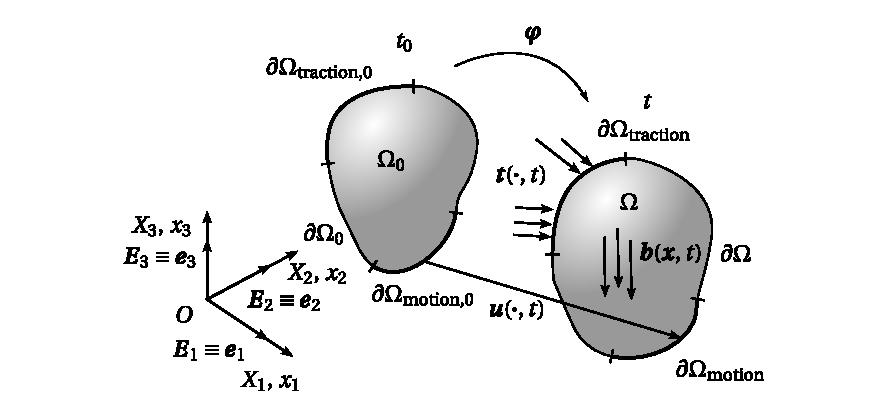
\includegraphics[width=.9\textwidth]{quasi_static_prob}
  \caption{Quasi-static mechanical constitutive initial boundary value problem.}
\label{fig:quasi_static_prob}
\end{figure}

It is also convenient to define the set of kinematically admissible displacements of $\mathscr{B}$ as the set of all sufficiently regular displacement functions tha satisfy the essential boundary condition \citep{de_souza_neto_computational_2008},
\begin{highlight}[innertopmargin=-5pt]
    \begin{multline}
        \mathscr{K}_u\equiv \{\vect u:\Omega_0\times \mathscr{R}\to \mathscr{U}\;|\;\vect u(\vect X,t) = \vect u_\text{presc} (\vect X,t),\\ \vect X\in\partial \Omega_\text{motion,0},\quad t\in [t_0,t_\text{end}]\}.\quad
    \end{multline}
\end{highlight}

So the weak form of the quasi-static mechanical constitutive initial boundary value problem can be stated in a spatial description as follows
\begin{problem}[Spatial mechanical initial BVP.]
    FFind a kinematically admissible displacement function, $\vect u\in \mathscr{K}_u$, such that for every $t\in [t_0,t_\text{end}]$, the body $\mathscr{B}$ is in equilibrium as stated by the Virtual Work Principle
        \begin{equation}
        \int_\Omega [\mat \sigma:\nabla \vect \eta - (\vect b-\rho\ddot{\bm u})\cdot \vect \eta]\ud v - \int_{\partial\Omega} \vect t\cdot \vect \eta\ud a = 0,\quad \forall \vect \eta \in \mathscr{V}_u,
    \end{equation}
    where the space of virtual displacements at time $t$ is defined by
    \begin{equation}
        \mathscr{V}_u \equiv \left\{\vect \eta:\Omega\to \mathscr{U}\;|\;\vect \eta = \vect 0\quad \text{in}\quad \bm \varphi(\partial\Omega_\text{motion,0},t)\right\},
    \end{equation}
    and at each point of $\mathscr{B}$, the Cauchy stress tensor is the solution of spatial mechanical constitutive initial values problem.
\end{problem}
and in the material description as
\begin{problem}[Material mechanical initial BVP.]
    FFind a kinematically admissible displacement function, $\vect u\in \mathscr{K}_u$, such that for every $t\in [t_0,t_\text{end}]$, the body $\mathscr{B}$ is in equilibrium as stated by the Virtual Work Principle
        \begin{equation}
        \int_{\Omega_0} [\mat P:\nabla_0 \vect \eta - (\vect b_0-\rho_0\ddot{\bm u})\cdot \vect \eta]\ud v - \int_{\partial\Omega_0} \vect t_0\cdot \vect \eta\ud a = 0,\quad \forall \vect \eta \in \mathscr{V}_{u,0},
    \end{equation}
    where the space of virtual displacements at time $t$ is defined by
    \begin{equation}
        \mathscr{V}_{u,0} \equiv \left\{\vect \eta:\Omega_0\to \mathscr{U}\;|\;\vect \eta = \vect 0\quad \text{in}\quad \partial\Omega_\text{motion,0}\right\},
    \end{equation}
    and at each point of $\mathscr{B}$, the First Piola-Kirchhoff stress tensor is the solution of material mechanical constitutive initial values problem.
\end{problem}

\section{Time discretization for the constitutive equations} \label{sec:time_discretization}

Given a generic path-dependent model, i.e., a model in which the stress state does not depend only on the instantaneous deformation state but also on the deformation history, the solution of the constitutive initial value problem for a given set of initial conditions is usually not known for complex strain paths $\mat F(t)$.
Thus, there is a need to use an appropriate numerical algorithm to integrate the rate constitutive equations.

In general, the algorithms for integrating rate constitutive equations are obtained adopting some time (or pseudo-time) discretization and some hypothesis on the deformation path between adjacent time stations.
In the present document, an algorithm is adopted based on approximated incremental constitutive functions.
Attending to the mechanical constitutive initial boundary value problem and considering the time increment $[t_n, t_{n+1}]$, this approach is comprised by the following two requirements:
\begin{itemize}
    \item \textbf{Cauchy and First Piola-Kirchhoff stress tensors.}   Considering a time increment $[t_n, t_{n+1}]$ and given the set $\vect \alpha_n$ of internal variables at $t_n$, the deformation gradient $\mat F_{n+1}$ at time $t_{n+1}$ determines the stress $\mat \sigma_{n+1}$ uniquely through
    \begin{highlight}
        \begin{equation}
            \mat \sigma_{n+1} = \hat{\mat \sigma}(\vect \alpha_n, \mat F_{n+1}), \label{eq:incremental_stress}
        \end{equation}
    \end{highlight}
    where $\hat{\vect \sigma}$ is the incremental constitutive function for the Cauchy stress tensor.

    Similarly, the First Piola-Kirchhoff stress tensor $\mat P_{n+1}$ must be uniquely determined by the prescribed deformation gradient $\mat F_{n+1}$ prescribed at $t_{n+1}$ as
    \begin{equation}
        \mat P_{n+1} = \hat{\mat P}(\mat \alpha_n, \mat F_{n+1}),
    \end{equation}
    where $\hat{\mat P}$ is the incremental constitutive function for the First Piola-Kirchhoff stress tensor.
    \item \textbf{Set of internal variables.} Assuming that the set of internal variables $\vect \alpha_n$ is known at $t_n$, the set of internal variables must be uniquely determined by the prescribed deformationgradient $\mat F_{n+1}$ prescribed at $t_{n+1}$ as
    \begin{highlight}
        \begin{equation}
             \vect \alpha_{n+1} =\hat{\vect \alpha}(\vect \alpha_n, \mat F_{n+1}), \label{eq:incremental_flux}
        \end{equation}
    \end{highlight}
    where $\hat{\vect \alpha}$ is the incremental constitutive function for the set of internal variables.
\end{itemize}

Generally, the numerical constitutive laws are nonlinear and path-independent within one increment.
In other words, within each increment, $\mat \sigma_{n+1}$ and $\vect \alpha_{n+1}$, they are functions of $\mat F_{n+1}$ alone with the argument $\vect \alpha_n$ constant within the same time interval.

Making use of the aforementioned time discretization, one can state the weak form of the mechanical constitutive initial boundary value problem in the spatial description as
\begin{problem}[Spatial incremental mechanical initial BVP.]
    GGiven the set of internal variables $\vect \alpha_n$ at $t_n$, the prescribed body and traction force fields $\vect b_{n+1}$ and $\vect t_{n+1}$ at $t_{n+1}$, and the prescribed deformating gradient $\mat F_{n+1}$ at $t_{n+1}$, find the kinematically admissible displacement field $\vect u_{n+1}\in\mathscr{K}_{u,n+1}$ such that the body $\mathscr{B}$ is in equilibrium as stated by the virtual Work Principle
            \begin{equation}
        \int_{\Omega_{n+1}} [\hat{\mat \sigma}(\mat F_{n+1}, \vect \alpha_n):\nabla \vect \eta - (\vect b_{n+1}-\rho\ddot{\bm u}_{n+1})\cdot \vect \eta]\ud v - \int_{\partial\Omega_{n+1}} \vect t_{n+1}\cdot \vect \eta\ud a = 0,\quad \forall \vect \eta \in \mathscr{V}_u,
    \end{equation}
    where the space of kinematically admissible displacement fields $\mathscr{K}_{n+1}$ is defined by
    \begin{equation}
            \mathscr{K}_{u,n+1}\equiv \{\vect u:\Omega_0\times \mathscr{R}\to \mathscr{U}\;|\;\vect u_{n+1}(\vect X) = \vect u_\text{presc,$n+1$}(\vect X),\;\vect X\in\partial \Omega_\text{motion,0}\}.
    \end{equation}
\end{problem}
and in the material description as
\begin{problem}[Material incremental mechanical initial BVP.]
    GGiven the set of internal variables $\vect \alpha_n$ at $t_n$, the prescribed body and traction force fields $\vect b_{0,n+1}$ and $\vect t_{0,n+1}$ at $t_{n+1}$, and the prescribed deformating gradient $\mat F_{n+1}$ at $t_{n+1}$, find the kinematically admissible displacement field $\vect u_{n+1}\in\mathscr{K}_{u,n+1}$ such that the body $\mathscr{B}$ is in equilibrium as stated by the virtual Work Principle
            \begin{equation}
        \int_{\Omega_0} [\hat{\mat P}(\mat F_{n+1}, \vect \alpha_n):\nabla_0 \vect \eta - (\vect b_{0,n+1}-\rho_0\ddot{\bm u}_{n+1})\cdot \vect \eta]\ud v - \int_{\partial\Omega_{0,n+1}} \vect t_{0,n+1}\cdot \vect \eta\ud a = 0,\quad \forall \vect \eta \in \mathscr{V}_{u,0},
    \end{equation}
    where the space of kinematically admissible displacement fields $\mathscr{K}_{n+1}$ is defined by
    \begin{equation}
            \mathscr{K}_{u,n+1}\equiv \{\vect u:\Omega_0\times \mathscr{R}\to \mathscr{U}\;|\;\vect u_{n+1}(\vect X) = \vect u_\text{presc,$n+1$}(\vect X),\;\vect X\in\partial \Omega_\text{motion,0}\}.
    \end{equation}
\end{problem}

\section{Finite Element Method} \label{sec:fem_mech}

With the incremental weak form of the mechanical constitutive initial boundary value problem now established, an approximated solution can be found using the Finite Element Method.

\subsection{Finite element concept}

The first in the Finite Element method is to discretize the continuum domain $\Omega$ in a finite set of $n_\text{elem}$ mutually exclusive subdomains called finite elements $\Omega^{(e)}$.
The discretized domain, $^h\Omega$, is therefore an approximation to the continuum domain expressed by
\begin{equation}
    \Omega \approx {}^h\Omega \equiv \bigcup_{e=1}^{n_\text{elem}}\Omega^{(e)}.
\end{equation}
The spaces of virtual displacements $\mathscr{V}_u$ and \(\mathscr V_{u,0}\) as well as the space of kinematically admissible displacement fields $\mathscr{K}_u$ are also discretized in the same way, with their discretized forms denoted by $^h\mathscr{V}_u$, \(^h\mathscr{V}_{u,0}\) and $^h\mathscr{K}_u$.

\subsection{Interpolation functions}

Let $e$ be a generic finite element with $n_\text{nodes}$ nodes, where each node $i$ of coordinates $\vect x^i$ is associated with an interpolation function $N_i^{(e)}$.
These interpolation functions are often called shape functions and perform the required filed interpolations inside the element domain $\Omega^{(e)}$.

Letting $a(\vect x)$ be a generic field defined over $\Omega^{(e)}$, its interpolation at any point $\vect x$ inside the element is defined by the element shape functions as
\begin{highlight}
    \begin{equation}
        a(\vect x) \approx {}^ha(\vect x) \equiv \sum_{i=1}^{n_\text{nodes}} a(\vect x_i) N_i^{(e)}(\vect x).
    \end{equation}
\end{highlight}
If instead $a(\vect x)$ is instead a generic field defined over the global domain $\Omega$, the interpolation of $a(\vect x)$ at any point $\vect x$ is defined by the global shape functions as
\begin{highlight}
    \begin{equation}
        a(\vect x) \approx {}^h a(\vect x) \equiv \sum_{i=1}^{n_\text{points}} a(\vect x_i) N_i^g(\vect x), \label{eq:interpol_global}
    \end{equation}
\end{highlight}
where $n_\text{points}$ is the total number of nodes of the finite element mesh.
The discretized spaces $^h \mathscr{V}_u$ and $^h\mathscr{K}_u$ can now be defined as
\begin{align}
    ^h \mathscr{K}_u&\equiv \Big\{\vphantom{|}^h\vect u(\vect x) = \sum_{i=1}^{n_\text{points}} \vect u(\vect x_i) N_i^g(\vect x)\;|\; \vect u(\vect x_i) = \vect u_\text{presc}(\vect x_i)\quad\text{if $\vect x_i\in \partial\Omega_\text{motion,0}$}  \Big\},\\
    ^h\mathscr{V}_u&\equiv \Big\{\vphantom{|}^h\vect \eta(\vect x) = \sum_{i=1}^{n_\text{points} } \vect \eta(\vect x_i) N_i^g(\vect x)\;|\;\vect \eta(\vect x_i)=\vect 0\quad\text{if $\vect x_i\in \partial\Omega_\text{motion,0}$}   \Big\}
\end{align}
Quantities defined on the reference configuration \(\Omega_0\) accepted a treatment entirely similar to the one described above, and thus is omitted.

\subsection{Interpolation matrix and discrete gradient operators}

The global shape functions can be conveniently assembled in the so-called global interpolation matrix as
\begin{equation}
    \mathbf N^g(\vect x) \equiv \left[\text{diag}[N_1^g(\vect x)]\; \text{diag}[N_2^g(\vect x)]\;\cdots\; \text{diag}[N_{n_\text{points}}^g(\vect x)]\right],
\end{equation}
where $\text{diag}[N_i^g]$ is a diagonal matriz $n_\text{dim} \times n_\text{dim}$
\begin{equation}
    \text{diag}[N_i^g(\vect x)]\equiv \left[
    \begin{array}{cccc}
         N_i^g & 0 & \cdots & 0  \\
         0     & N_i^g & \cdots & 0 \\
         \vdots & \vdots & \ddots & \vdots \\
         0 & 0 & \cdots & N_i^g
    \end{array}
    \right]
\end{equation}
where $n_\text{dim}$ is the number of degrees of freedom per node.

Defining the global vector of nodal displacements as
\begin{equation}
    \mathbf u = \Big[ u_1^1,\dots,u^1_{n_\text{dim}},\dots, u_1^{n_\text{points}},\dots,u^{n_\text{points}}_{n_\text{dim}}\Big]^T,
\end{equation}
the displacement field $\bm u(\vect x)$ defined over the global domain $\Omega$, can be found from Equation \eqref{eq:interpol_global} at any point $\vect x$ as
\begin{highlight}
    \begin{equation}
        ^h\vect u(\vect x) \equiv \mathbf N^g(\vect x)\mathbf u,\quad {}^h\vect u\in {}^h\mathscr{K}_u.
    \end{equation}
\end{highlight}

\subsection{Spatial discretization} \label{sec:spatial_discretization_mech}

Applying the aforementioned finite element discretization to the incremental mechanical constitutive initial boundary value problem, we can then write in the spatial description
\begin{highlight}
    \begin{equation}
        \int_{^h\Omega}\left[\hat{\mat \sigma}^T\mathbf B^g\vect \eta - (\mathbf b_{n+1} - \rho\ddot{\mathbf u}_{n+1}) \cdot \mathbf N^g \vect \eta \right]\ud v -\int_{\partial ^h\Omega_\text{traction}} \mathbf t_{n+1}\cdot \mathbf N^g\vect \eta \ud a = 0,\quad \forall \vect \eta \in {}^h\mathscr{V}_u,  \label{eq:forma_fraca_disc}
    \end{equation}
\end{highlight}
where $\mathbf B^g$ is the discrete symmetric global gradient operator, defined for a 2D problem in cartesian coordinates as
\begin{equation}
    \mathbf B^g\equiv \left[
    \begin{array}{ccccccc}
         \displaystyle{\frac{\partial N_1^g}{\partial x}} & 0 & \displaystyle{\frac{\partial N_2^g}{\partial x}} & 0 & \cdots &
         \displaystyle{\frac{\partial N_{n_\text{points}}^g}{\partial x}} & 0\\
         0 & \displaystyle{\frac{\partial N_1^g}{\partial y}} & 0 & \displaystyle{\frac{\partial N_2^g}{\partial y}} & \cdots &
         0 & \displaystyle{\frac{\partial N_{n_\text{points}}^g}{\partial y}}\\
         \displaystyle{\frac{\partial N_1^g}{\partial y}} & \displaystyle{\frac{\partial N_1^g}{\partial x}} & \displaystyle{\frac{\partial N_2^g}{\partial y}} & \displaystyle{\frac{\partial N_2^g}{\partial x}} & \cdots &
         \displaystyle{\frac{\partial N_{n_\text{points}}^g}{\partial y}} & \displaystyle{\frac{\partial N_{n_\text{points}}^g}{\partial x}}
    \end{array}
    \right].
\end{equation}

Equation \eqref{eq:forma_fraca_disc} can be rewritten as
\begin{multline}
    \left\{  \int_{^h\Omega}\left[{\mathbf B^g}^T \hat{\mat \sigma}(\vect \alpha_n, \vect F_{n+1})-{\mathbf N^g}^T\mathbf b_{n+1} +{\mathbf N^g}^T\rho\ddot{\mathbf u}_{n+1} \right]\ud v \right. \\ \left. -\int_{\partial ^h\Omega_\text{traction}} {\mathbf N^g}^T \mathbf t_{n+1}\ud a\right\}^T\;\vect \eta =0,\quad \forall \vect \eta \in ^h \mathscr{V}_u, \label{eq:eq_forças}
\end{multline}
and, since it must be satisfied for any $\vect \eta \in {}^h \mathscr{V}_u$, the incremental quasi-static discretized mechanical constitutive initial boundary value problem can thus be stated in the spatial description as
\begin{problem}[Spatial incremental discretized mechanical initial BVP.]
GGiven the set of internal variables $\vect \alpha_n$ at $t_n$, the prescribed body and traction force fields $\vect b_{n+1}$ and $\vect t_{n+1}$, and the prescribed deformation gradient $\mat F_{n+1}$ at $t_{n+1}$, find the kinematically admissible nodal displacement field $\vect u_{n+1}\in {^h\mathscr{K}_{u,n+1}}$ such that the body $\mathscr{B}$ is in equilibrium as stated by the Virtual Work Principle
\begin{equation}
    \mathbf M \ddot{\mathbf u}_{n+1} + \mathbf f^\text{\;int}(\mathbf u_{n+1})-\mathbf f^\text{\;ext}_{n+1}=\mathbf 0, \label{eq:equilibrium_spatial}
\end{equation}
where $\mathbf f^\text{int}$ e $\mathbf f^\text{ext}_{n+1}$ are the global vectors of internal and external forces defined as
\begin{align}
    \mathbf f^\text{\;int} &\equiv \int_{^h\Omega}{\mathbf B^g}^T \hat{\mat \sigma}(\mat F_{n+1}, \vect \alpha_n)\ud v,\\
    \mathbf f^\text{\;ext}_{n+1} &\equiv \int_{^h\Omega}{\mathbf N^g}^T \mathbf b_{n+1}\ud v + \int_{\partial^h\Omega_\text{traction}}{\mathbf N^g}^T \mathbf t_{n+1}\ud a,
\end{align}
and $\mathbf M$ is the mass matrix defined as
\begin{equation}
  \mathbf M = \int_{{}^h\Omega} \rho {\mathbf{N}^g}^T\mathbf{N}^g \ud v.
\end{equation}
\end{problem}
In a material description, Equation \eqref{eq:eq_forças} is written as
\begin{multline}
     \left\{  \int_{^h\Omega_0}\left[{\mathbf G^g}^T \hat{\mat P}(\vect \alpha_n, \vect F_{n+1})-{\mathbf N^g}^T \mathbf b_{0,n+1} + {\mathbf N^g}^T \rho_0\ddot{\mathbf u}_{n+1} \right]\ud v \right.\\ \left.   -\int_{\partial ^h\Omega_\text{traction,0}} {\mathbf N^g}^T \mathbf t_{0,n+1}\ud a\right\}^T\;\vect \eta =0,\quad \forall \vect \eta \in ^h \mathscr{V}_{u,0},
\end{multline}
where $\mathbf G^g$ is the discrete global gradient operator, defined for a 2D problem in cartesian coordinates as
\begin{equation}
    \mathbf G^g\equiv \left[
    \begin{array}{ccccccc}
         \displaystyle{\frac{\partial N_1^g}{\partial x}} & 0 & \displaystyle{\frac{\partial N_2^g}{\partial x}} & 0 & \cdots &
         \displaystyle{\frac{\partial N_{n_\text{points}}^g}{\partial x}} & 0\\
         0 & \displaystyle{\frac{\partial N_1^g}{\partial x}} & 0 & \displaystyle{\frac{\partial N_2^g}{\partial x}} & 0 & \cdots &
         \displaystyle{\frac{\partial N_{n_\text{points}}^g}{\partial x}}\\
         \displaystyle{\frac{\partial N_1^g}{\partial y}} & 0 & \displaystyle{\frac{\partial N_2^g}{\partial y}} & \cdots &
         0 & \displaystyle{\frac{\partial N_{n_\text{points}}^g}{\partial y}} & 0\\
         0 & \displaystyle{\frac{\partial N_1^g}{\partial y}} & 0 & \displaystyle{\frac{\partial N_2^g}{\partial y}} & \cdots &
         0 & \displaystyle{\frac{\partial N_{n_\text{points}}^g}{\partial y}}\\
    \end{array}
    \right],
\end{equation}
and, as for the spatial description, it must  be satisfied for any $\vect \eta \in {}^h\mathscr{V}_{u,0}$, the incremental quasi-static discretized mechanical constitutive initial boundary value problem can thus be stated in the material description as
\begin{problem}[Material incremental discretized mechanical initial BVP.]
GGiven the set of internal variables $\vect \alpha_n$ at $t_n$, the prescribed body and traction force fields $\vect b_{0,n+1}$ and $\vect t_{0,n+1}$, and the prescribed deformation gradient $\mat F_{n+1}$ at $t_{n+1}$, find the kinematically admissible nodal displacement field $\vect u_{n+1}\in {^h\mathscr{K}_{u,n+1}}$ such that the body $\mathscr{B}$ is in equilibrium as stated by the Virtual Work Principle
\begin{equation}
    \mathbf M \ddot{\mathbf u}_{n+1} +\mathbf f^\text{\;int}(\mathbf u_{n+1})-\mathbf f^\text{\;ext}_{n+1}=\mathbf 0, \label{eq:equilibrium_material}
\end{equation}
where $\mathbf f^\text{\;int}$ e $\mathbf f^\text{\;ext}_{n+1}$ are the global vectors of internal and external forces defined as
\begin{align}
    \mathbf f^\text{int} &\equiv \int_{^h\Omega_0}{\mathbf G^g}^T \hat{\mat P}(\mat F_{n+1}, \vect \alpha_n)\ud v,\\
    \mathbf f^\text{ext}_{n+1} &\equiv \int_{^h\Omega_0}{\mathbf N^g}^T \mathbf b_{0,n+1}\ud v + \int_{\partial^h\Omega_\text{traction,0}}{\mathbf N^g}^T \mathbf t_{0,n+1}\ud a.
\end{align}
and $\mathbf M$ is the mass matrix defined as
\begin{equation}
  \mathbf M = \int_{{}^h\Omega_0} \rho_0 {\mathbf{N}^g}^T\mathbf{N}^g \ud v.
\end{equation}
\end{problem}

The global vectors for the internal and external forces are usually obtained by assemblage of their elemental counterparts as
\begin{gather}
    \mathbf f^\text{\;int} = \assemble_{e=1}^{n_\text{elem}} \left(\mathbf f^\text{\;int}\right)^{(e)},\\
    \mathbf f^\text{\;ext} = \assemble_{e=1}^{n_\text{elem}} \left(\mathbf f^\text{\;ext}\right)^{(e)},
\end{gather}
where the elemental vectors in the spatial description are defined as
\begin{highlight}[innertopmargin=-5pt]
    \begin{align}
        \left(\mathbf f^\text{\;int}\right)^{(e)} &\equiv \int_{^h\Omega^{(e)}} \mathbf B^T \hat{\mat \sigma }(\mat F_{n+1},\mat \alpha_n)\ud v,\\
        \left(\mathbf f^\text{\;ext}_{n+1}\right)^{(e)} &\equiv \int_{^h\Omega^{(e)}}\mathbf N^T \mathbf b_{n+1}\ud v + \int_{\partial^h\Omega_\text{traction}^{(e)}} \mathbf N^T \mathbf t_{n+1}\ud a,
    \end{align}
\end{highlight}
and in material description as
    \begin{align}
        \left(\mathbf f^\text{\;int}\right)^{(e)} &\equiv \int_{^h\Omega_0^{(e)}} \mathbf G^T \hat{\mat P }(\mat F_{n+1},\mat \alpha_n)\ud v,\\
        \left(\mathbf f^\text{\;ext}_{n+1}\right)^{(e)} &\equiv \int_{^h\Omega_0^{(e)}}\mathbf N^T \mathbf b_{0,n+1}\ud v + \int_{\partial^h\Omega_\text{0, traction}^{(e)}} \mathbf N^T \mathbf t_{0,n+1}\ud a,
    \end{align}
The matrices $\mathbf N$, $\mathbf B$, and $\mathbf G$ are the elemental interpolation matrix, the symmetric elemental gradient operator, and the discrete elemental gradient operator.

In a similar manner, the global mass matrix is also usually obtained by assemblage of their elemental counterparts as
\begin{equation}
  \mathbf M \equiv \assemble_{e=1}^{n_\text{elem}} \mathbf M^{(e)},
\end{equation}
where the elemental mass matrices in the spatial description are defined as
\begin{highlight}
  \begin{equation}
    \mathbf M^{(e)} = \int_{^h\Omega^{(e)}} \rho \mathbf N^T\mathbf N\ud v,
  \end{equation}
\end{highlight}
and the material descriptrion
\begin{equation}
  \mathbf M^{(e)} = \int_{^h\Omega_0^{(e)}} \rho_0\mathbf N^T\mathbf N \ud v.
\end{equation}

\subsection{Numerical integration} \label{sec:numerical_integration}

In the Finite Element Method, the integrations over the element domain are generally performed numerically using the Gaussian Quadrature Method.
Stating it's application succinctly, let $a(\vect x)$ be a generic field, if there is a coordinate transformation from a local (or natural) normalized domain $\Upsilon$ to the element domain $\Omega^{(e)}$, $\vect x\colon \Upsilon \to \Omega^{(e)}$, the integral of $a(\vect x)$ over the domain $\Omega^{(e)}$ can be numerically determined as
\begin{equation}
    \int_{\Omega^{(e)} } a(\vect x)\ud \vect x = \int_\Upsilon a(\vect x(\vect \zeta))j(\vect \zeta)\ud \vect \zeta \approx \sum_{i=1}^{n_\text{GP}} w_i a(\vect x(\vect \zeta_i))j(\vect \zeta_i),
\end{equation}
where $\vect \zeta_i$ and $w_i$, $i=1,\dots,n_\text{GP}$ are the positions and weigths of the Gauss sampling points in the domain $\Upsilon$ and $j(\vect \zeta)$ is the determinant of the coordinate trasnformation's Jacobian defined as
\begin{equation}
    j(\vect \zeta) = \text{det}\,\left(\frac{\partial \vect x}{\partial \vect \zeta}\right).
\end{equation}

\section{Time discretization}

The space-discrete time-continuous equilibrium equations can be integrated by employing an adequate and robust time discretization scheme.
In the present work the time integration method employed is an implicit linear multistep (LMS) method, the so-called generalised-\(\alpha\) method, originally proposed by \cite{chung1993time}.
It rests on the discretisation of the time domain into subintervals with duration \(\Delta t=t_{m+1}-t_n\), such that the time derivatives are approximated by appropriate finite differences and the equilibrium equations are satisfied at the discrete time step \(t_{n+1}\).

\newpage\null\thispagestyle{blank}\newpage

% \section{Linearisation}
%
% The equilibrium equation, Equation \eqref{eq:equilibrium_spatial} in a spatial description and Equation \eqref{eq:equilibrium_material} in a material description, is generally nonlinear due to geometrical and/or material nonlinearities.
% The Newton-Raphson Method is an efficient and robust iterative scheme with a quadratic convergence rate often used to solve the equilibrium equation at each time increment, $t_n$.
% The residual of the fully discretized balance of linear momentum is defined for an iteration step \(i\) of the Newton-Raphson method as
% \begin{equation}
% \mathbf{r}(\mathbf{u}_{n+1}^{i})=\mathbf{M} \ddot{\mathbf u}_{n+1}^{i}+\mathbf f^\text{\;int} (\mathbf{u}_{n+1}^{i})-\mathbf{f}_{n+1}^\text{\;ext}.
% \end{equation}
% A Taylor expansion about the current solution \(\mathbf{u}_{n+1}^{i}\) is performed, discarding all terms of  higher order than one, yielding the linearised form
% \begin{equation}
% \operatorname{Lin} \mathbf{r}(\mathbf{u}_{n+1}^{i})=\mathbf{r}(\mathbf{u}_{n+1}^{i})+\underbrace{\left.\frac{\partial \mathbf{r}(\mathbf{u}_{n+1})}{\partial \mathbf{u}_{n+1} }\right|^{i} }_{\mathbf{K}(\mathbf{u}_{n+1}^{i})} \delta \mathbf{u}.
% \end{equation}
% with the dynamic effective tangential stiffness matrix \(\mathbf{K}(\mathbf{u}_{n+1}^{i})\).
% The linearisation of the internal forces included in \(\mathbf{K}\) is known as the tangential stiffness matrix \(\mathbf{K}_T\), which is defined as
% \begin{equation}
% \mathbf{K}_{T}^{i}=\left.\frac{\partial \mathbf{f}^{\text{\;int}} }{\partial \mathbf{u}_{n+1}}\right|^{i}.
% \end{equation}
% Equilibrium is achieved if
% \begin{equation}
% \operatorname{Lin} \mathbf{r}(\mathbf{u}_{n+1}^{i}) = \mathbf{0},
% \end{equation}
% so that a linear system of equation is given by
% \begin{equation}
% \mathbf{K}(\mathbf{u}_{n+1}^{i}) \delta \mathbf{u}=-\mathbf{r}\left(\mathbf{u}_{n+1}^{i}\right).
% \end{equation}
% Thus, a new solution of the displacement increment \(\delta \mathbf{u}\) for current iteration step \(i+1\) is determined, and the final displacement solution of time step \(n+1\) is obtained via updating
% \begin{equation}
% \mathbf{u}_{n+1}^{i+1}=\mathbf{u}_{n+1}^{i}+\delta \mathbf{u}.
% \end{equation}
% A solution of \(t_{n+1}\) is found, i.e. an equilibrium state is reached and \(\mathbf{u}_{n+1}=\mathbf{u}_{n+1}^{i+1}\), if prescribed, user-defined convergence criteria are fulfilled.
%
%
%
% \section{Constitutive laws}

\chapter{Thermo field}

For the development of the thermomechanical models, the temperature field needs to be considered.
This section provides an overview of the governing equations required to describe a temperature field with the finite element method (FEM).
The procedure to establish a fully discrete system of equations for the themal field is comparable to the one for the structural field in chapter~\ref{}.
Furthermore, the basics of nonlinear continuum thermodynamics have already been featured in chapter~\ref{}.
Consequently, the detailed derivation are skipped in this chapter.

% In a first step, the balance equations for the thermal field will be established. Then, in a second step the thermal initial boundary value problem (IBVP) will be presented followed by the numerical solution technique. Latter requires a weak form of the thermal balance equation which will be fully discretised using the FEM for space discretisation and the finite difference method for time discretisation. To finish, the residual and the tangential system matrix will be introduced to enable the application of a Newton-Raphson method.

\section{Governing equations}

Based on the general model presented in Section~\ref{}, the balance equations for the temperature field are obtained as a special case by neglecting all mechanical terms.
Hence, the energy balance equation (Equation~\eqref{eq:first_principle_thermo}), now in material description, reduces to
\begin{equation} \label{eq:strong_energy_eq}
\rho_0\ e=-\operatorname{div}_0 \bm q_0+\rho_0 r \quad \text { in } \Omega_0,
\end{equation}
where all mechanical terms are neglected.
The target application of the present work are coupled generally nonlinear thermomechanical interaction problems, where the initial and the current domains are not equal, i.e. \(\Omega_{0} \neq \Omega\).
Thus, for the sake of simplicity and in view of the later coupled problem, all following relations are expressed in material quantities.
A purely thermal analysis is independent of the deformation, so that reference and current configuration are identical and the domain remains constant, i.e. \(\Omega_{0} \equiv \Omega\).

\section{Thermal constitutive initial value problem}

From Section~\ref{}, discarding all variables related to the mechanical problem, the general thermal constitutive initial value problem is
\begin{problem}[General thermal constitutive intial value problem.]
GGiven the initial value of the internal variables \(\bm \alpha(t_0)\) and the history of the temperature distribution
\[\theta(t),\quad t\in[t_0, t_\text{end}],\]
find the function for $\bm q_0(t)$, \(s(t)\) and \(\bm \alpha(t)\) such that the constitutive equations
\begin{gather}
    s = -\frac{\partial \psi}{\partial \theta},\label{eq:entropy_constitutive_relation}\\
    \psi = \psi(\theta),\\
    \dot{\bm \alpha} = f(\theta, \bm g_0, \bm \alpha),\\
    \frac{1}{\theta}\bm q_0 = g(\theta, \bm g_0, \bm \alpha).
\end{gather}
are satisfied for every $t\in [t_0, t_\text{end}]$.
\end{problem}
No distinction between spatial and material configurations applies as \(\Omega = \Omega_0\).
Next, a standard set of assumptions are introduced.

\paragraph{Helmholtz free energy}
As a first step, the specific heat \(C_{V}\) is established and defined according to the thermodynamical principles to be the amount of heat required to change a unit mass of a substance by one degree in temperature, i.e.
\begin{equation}
C_{\mathrm{V}}=\frac{\partial e}{\partial \theta}.
\end{equation}
The index \((\cdot)_\mathrm{V}\) denotes that \(C_\mathrm{V}\) is measured at constant volume.
Its dimensions are energy over temperature, i.e., \(\mathrm{[E/\Theta]}\), and using the International System of Units (SI), \(C_{V}\) is expressed in joule per kelvin.
Using Equation~\ref{eq:def_helmholtz_free_energy}, the specific heat at constant volume can be written as
\begin{equation} \label{eq:def_cv_partial}
C_{\mathrm{V}}=-\frac{\partial^{2} \psi}{\partial \theta^{2}} \theta=\frac{\partial s}{\partial \theta} \theta.
\end{equation}
In general, the heat capacity depends on the deformation and on the temperature.
A substance whose specific volume (or density) is constant is called an incompressible substance.
This incompressibilty or constant-volume assumption should be taken to imply that the energy associated with the volume change is negligible compared with other forms of energy.
For the application to elastomers, see for instance Netz [96], the heat capacity \(C_{V}\) can be assumed to depend only on the temperature, and the partial derivatives in Equation~\eqref{eq:def_cv_partial} turn into exact derivatives, yielding
\begin{equation}
  C_\mathrm{V} = \frac{\ud s}{\ud \theta}\theta.
\end{equation}
Furthermore, for the application to metals, a constant specific heat capacity (i.e. \(C_{\mathrm{V}}=\) const.) is a valid assumption, utilised e.g. in Adam and Ponthot [1], Ghadiani [48], Ibrahimbegovic and Chorfi [61], and Simo and Miehe [122].
Accordingly, the heat capacity is also assumed to be constant (i.e. \(C_{\mathrm{V}}= \mathrm{const}\).), since focus in this work is on the application to metals.
Thus, the entropy can be written as
\begin{highlight}
\begin{equation}
s(\theta) = C_\mathrm{V}\ln\left(\frac{\theta}{\theta_0}\right),
\end{equation}
\end{highlight}
after integration, where \(\theta_{0}\) and \(C_{\mathrm{V}}\) denote the constant initial temperature and the constant specific heat, respectively.

Given the constituive relation for the entropy (Equation~\eqref{eq:entropy_constitutive_relation}), the Helmholtz free energy per unit reference volume is found to be
\begin{highlight}
\begin{equation}
\psi(\theta)=- C_{\mathrm{V}}\left[\left(\theta-\theta_{0}\right)-\theta \ln \left(\frac{\theta}{\theta_{0}}\right)\right],
\end{equation}
\end{highlight}
Subsequently, the time derivative of the entropy is
\begin{equation}
\dot{s}(\theta)=\frac{\partial s}{\partial \theta} \dot{\theta}=-\frac{\partial^{2} \psi}{\partial \theta^{2}} \dot{\theta}=C_{\mathrm{V}} \frac{1}{\theta} \dot{\theta}.
\end{equation}

\paragraph{Law for the heat flux}
As previously mentioned, in a purely thermal analysis the deformation is neglected, consequently the material and spatial heat flux coincide, that is \(\bm q_0 \equiv \bm q\), which is also valid for the material and spatial gradient, hence \(\nabla_0 \theta = \nabla \theta\).
To satisfy the dissipation inequality due to conduction (Equation~\eqref{}), a constitutive law for the heat flux has to be chosen associating the heat flux \(\bm q_0\) with its dual variable \(\bm g_0\) and the temperature \(\theta\).
Accordingly, so-called Fourier's law, which is linear and isotropic is utilised, which is defined as
\begin{highlight}
\begin{equation}
  \bm q_0=-k \bm g_0.
\end{equation}
\end{highlight}
Herein, the thermal conductivity \(k\) is assumed constant and positive that is \(k \geq 0\).
Thus, heat is conducted in the direction of decreasing temperatures.
Apart from Fourier's law, different constitutive laws for the heat flux are available in the literature, as e.g. Duhamel's law of heat conduction (see e.g. \cite{}Holzapfel [58]) which uses a positive semi-definite second-order tensor \(k\) instead of the constant conductivity \(k\).
If Duhamel's law is restricted to thermally isotropic behaviour (i.e. no preferred direction), the conductivity tensor reduces to \(k=k \boldsymbol{I}\).
If a constant heat conductivity \(k=\) const. is assumed, Fourier's law is recovered as a special form of Duhamel's law.
Moreover, e.g. in Holzapfel and Simo [59] and Sherief and Abd El-Latief [117], a variable conductivity \((k \neq \mathrm{const}\) is assumed in the context of elastomers).
In Bargmann and Steinmann [13] and Bargmann et al. [14], three different constitutive laws for the heat flux \(\bm q\) are proposed based on the Green-Naghdi's non-classical theory.
Nevertheless, for the present work Fourier's law yields physical results and hence is exclusively considered in this work.

\paragraph{"Standard" thermal constitutive description}
No extra internal variables \(\bm \alpha\) are considered in the present description of the thermal problem.
Thus, the thermal constitutive initial value problem given the standard assumptions laid out above accepts a closed form solution, i.e., the functions for \(\bm q\) and \(s\) are known from the outset.

\begin{problem}["Standard" thermal constitutive description]
GGiven the history of the temperature distribution
\[\theta(t),\quad t\in[t_0, t_\text{end}],\]
compute the functions for $\bm q_0(t)$ and \(s(t)\) at every $t\in [t_0, t_\text{end}]$ using the constitutive equations
\begin{gather}
    s =C_{\mathrm{V}} \ln \left(\frac{\theta}{\theta_{0}}\right),\\
    \bm q_0 = -k\bm g_0.
\end{gather}
\end{problem}

\section{Weak energy balance equation}

The solution of the thermal problem using the FEM requires the use of the weak form of the energy balance equation.
Applying to the governing equation (Equation~\eqref{eq:strong_energy_eq}) in the strong form, a variational approach, multiplying it by the virtual temperatures \(\xi\) followed by integration by parts, one can find the energy balance equation in its weak form.
\begin{problem}[Weak energy balance equation]
TThere is energy balance in the body if and only if the temperature distribution satisfies
    \begin{equation}
        \int_{\Omega_0}   \left[\left(\dot e - \rho_0 r\right) \xi - \bm q_0\cdot \nabla_0 \xi\right]\ud v - \int_{\partial\Omega_0} h_0 \xi\ud a = 0,\quad \forall \xi \in \mathscr{V}_{\theta,0},
    \end{equation}
 where $\mathscr{V}_{\theta,0}$ is the space of virtual temperature distributions on the body, defined by the space of sufficiently regular arbitrary temperature distributions.
 \end{problem}

\section{The thermal initial boundary value problem}

Following the same approach as in Section~\ref{}, it is now possible to introduce the the thermal initial boundary value problem.
Assume that the internal variables governing the body \(\mathcal B\) are known at the initial time \(t_0\).
In addition, assume that the heat generated in the interior of the body is prescribed, \(r(\bm X, t)\), \(t\in[t_0, t_\text{end}]\), as well as,
\begin{itemize}
  \item \textbf{Natural (or Neumann) boundary condition.} The boundary portion \(\partial \Omega_\text{heat,0}\) of \(\mathcal B\) is subject to a prescribed history of heat flux, \(h_\text{presc,0}(\bm X, t) = \bm q_\text{presc,0}(\bm X, t)\cdot \bm m(\bm X)\), \(\bm X \in \partial \Omega_\text{heat,0}\), \(t\in [t_0,t_\text{end}]\).
  \item \textbf{Essential (or Dirichlet) boundary condition.} The boundary portion \(\partial \Omega_\text{temperature,0}\) of \(\mathcal B\) is subject to a prescribed temperature history, \(\theta_\text{presc}(\bm X, t)\), \(\bm X \in \partial \Omega_\text{temperature,0}\), \(t\in [t_0,t_\text{end}]\).
\end{itemize}

As before the admissible temperature distributions for the body \(\mathcal B\) are all sufficiently regular temperature fields that satisfy the essential boundary condition,
\begin{equation}
  \mathscr K_\theta = \{\theta:\Omega_0 \times \mathbb R \to \mathbb R\,|\,\theta(\bm X, t) = \theta_\text{presc}(\bm X, t),\quad \bm X\in \partial \Omega_\text{temperature,0},\quad t\in[t_0, t_\text{end}]\}.
\end{equation}

Combining the weak energy balance equations with the "standard" thermal constitutive description, the weak form of the "standard" thermal constitutive initial boundary value problem can be stated as follows
 \begin{problem}["Standard" thermal initial BVP.]
     FFind an admissible temperature distribution, $\theta \in \mathscr{K}_\theta$, such that for every $t\in [t_0,t_\text{end}]$, the body $\mathscr{B}$ is in energetic equilibrium
         \begin{equation}
         \int_{\Omega_0}   \left[\left(C_\mathrm{V} \dot \theta - \rho_0 r\right) \xi +k\bm g_0\cdot \nabla_0 \xi\right]\ud v - \int_{\partial\Omega_0} h_0 \xi\ud a = 0,\quad \forall \xi \in \mathscr{V}_{\theta,0},
     \end{equation}
     where the space of virtual temperature distributions at time $t$ is defined by
     \begin{equation}
         \mathscr{V}_{\theta,0} \equiv \left\{\xi:\Omega_0\to \mathbb R\;|\;\xi = 0\quad \text{in}\quad \partial\Omega_\text{temperature,0}\right\}.
     \end{equation}
 \end{problem}

\section{Finite Element Method}

Following a procedure entirely similar to the one described in Section~\ref{}, the global shape functions can be conveniently assembled in the so-called global interpolation matrix as
\begin{equation}
\mathbf{N}^{g}(\boldsymbol{X}) \equiv\left[N_1^g(\bm X), N_2^g(\bm X), \dots, N^g_{n_\text{points}}(\bm X)\right].
\end{equation}

The vector containg the nodal values of the temperature is denoted by \(\bm \uptheta\) and defined as
\begin{equation}
 \bm \uptheta (t)= \left[\theta^{1}(t), \dots, \theta^{n_{\text {points}}}(t)\right]^{T},
\end{equation}
such that the value of the temperature inside the descretized domain \(^h\Omega_0\) can be found from
\begin{highlight}
\begin{equation}
{ }^{h} \theta(\bm{X},t) \equiv \mathbf{N}^{g}(\bm{X}) \bm{\uptheta}(t), \quad{ }^{h} \theta \in{ }^{h} \mathscr{K}_\theta.
\end{equation}
\end{highlight}

It is also convenient to defined the discrete gloabal gradient operator \(\mathbf H^g\).
For instance, in a 2D problem, where cartesian coordinates are employed, this discrete operator is defined as
\begin{equation}
  \mathbf H^g\equiv \left[
  \begin{array}{cccc}
    \displaystyle{\frac{\partial N^g_1}{\partial X}} & \displaystyle{\frac{\partial N^g_2}{\partial X}} & \dots & \displaystyle{\frac{\partial N^g_{n_\text{points}}}{\partial X}} \\[10pt]
    \displaystyle{\frac{\partial N^g_1}{\partial Y}} & \displaystyle{\frac{\partial N^g_2}{\partial Y}} & \dots & \displaystyle{\frac{\partial N^g_{n_\text{points}}}{\partial Y}}
  \end{array}
  \right].
\end{equation}

Applying the aforementioned finite element discretization to the "standard" thermal initial BVP yields
\begin{highlight}
\begin{equation}
  \int_{^h\Omega_0}   \left[\left(C_\mathrm{V} \dot \theta - \rho_0 r\right)  \mathbf N^g\bm \upxi +k\bm g_0\cdot \mathbf H^g \bm \upxi\right]\ud v - \int_{^h\partial\Omega_0} h_0 \mathbf N^g\bm \upxi\ud a = 0,\quad \forall \bm \upxi \in {}^h\mathscr{V}_{\theta,0},
\end{equation}
\end{highlight}
which can be rewritten
\begin{equation} \label{eq:thermo_variational_lemma}
  \left\{\int_{^h\Omega_0}   \left[(\mathbf N^g)^T\left(C_\mathrm{V} \dot \theta - \rho_0 r\right) +k(\mathbf H^g)^T\mathbf H^g \bm \uptheta \right]\ud v - \int_{^h\partial\Omega_0} (\mathbf N^g)^T h_0 \ud a \right\}^T\bm \upxi= 0,\quad \forall \bm \upxi \in {}^h\mathscr{V}_{\theta,0},
\end{equation}
where the relation \(\bm g_0 = \mathbf H^g \bm \uptheta\) is employed.
Since Equation~\eqref{eq:thermo_variational_lemma} must be satisfied for any \(\bm \upxi\in {}^h\mathscr V_{\theta,0}\), the discretized "standard" thermal initial boundary value problem can be statted as
\begin{problem}[Discretized "standard" thermal initial BVP.]
GGiven the prescribed heat sources and heat fluxes $r(\bm X, t)$ and $h_0(\bm X, t)$ find the admissible nodal temperatures $\theta(t)\in {^h\mathscr{K}_{\theta}}$ such that the body $\mathscr{B}$ is in energetic equilibrium
\begin{equation}
    \mathbf C \dot{ \bm\uptheta}(t) +\mathbf K\bm\uptheta(t)-\mathbf f^\text{\;ext}(t)=\mathbf 0, \label{eq:equilibrium_material}
\end{equation}
where $\mathbf C$ and \(\mathbf K\) are the temperature damping and stiffness matrix defined as
\begin{align}
  \mathbf C &= \int_{{}^h\Omega_0} C_\mathrm{V} {\mathbf{N}^g}^T \mathbf{N}^g \ud v.,\\
  \mathbf K &= \int_{{}^h\Omega_0} k {\mathbf{H}^g}^T\mathbf{H}^g \ud v.
\end{align}
and $\mathbf f^\text{\;ext}(t)$ is the global vector of external forces defined as
\begin{align}
    \mathbf f^\text{\;ext}(t) &\equiv \int_{^h\Omega_0} \rho{\mathbf N^g}^T r(\bm X, t)\ud v + \int_{\partial^h\Omega_\text{heat,0}}{\mathbf N^g}^T h_0(\bm X, t)\ud a.
\end{align}
\end{problem}

\chapter{Mechanical problem}

In the following chapter, the general framework presented in the previous chapter is applied to a purely mechanical analysis, neglecting the thermal terms.

\subsection{Mechanical constitutive initial value problem}

In the purely mechanical case, with all the quantities related to the thermal domain removed, a constitutive model based on internal variables is established by the following set of equations
    \begin{gather}
        \mat P = \rho_0 \frac{\partial \psi}{\partial \mat F},\\
        s = - \frac{\partial \psi}{\partial \theta},\\
        \psi = \psi(\mat F,\theta, \nabla_0 \theta,\mat \alpha),\\
        \dot{\vect \alpha} = f(\mat F, \theta, \nabla_0 \theta,\vect \alpha),\\
        \frac{1}{\theta}\nabla_0 \theta = g(\bm F, \theta, \bm \alpha).
    \end{gather}
  Thus, the spatial mechanical constitutive initial value problem can be stated as follows

  the single effects. To emphasize this additive decomposition, the Helmholtz free energy \(\psi\) in (5.7) is expressed with respect to the reference volume, so that \(\psi\) is reformulated using potential functions according to
  \[
  \rho_{0} \psi\left(\boldsymbol{F}, T, \operatorname{grad} T, \boldsymbol{\alpha}_{\mathrm{k}}, \boldsymbol{X}\right):=\hat{\mathbb{U}}\left(J^{e}\right)+\hat{\mathbb{W}}(\tilde{\boldsymbol{F}})+\hat{\mathbb{M}}\left(J^{e}, T\right)+\hat{\mathbb{T}}(T)+\hat{\mathbb{K}}\left(\boldsymbol{\alpha}_{k}, T\right)
  \]
  where in contrast to the deformation gradient \(\boldsymbol{F}\), the Jacobi-determinant \(J^{e}(5.6)\) and the isochoric deformation gradient \(\tilde{\boldsymbol{F}}(2.36)\) are applied. \(\hat{U}\) and \(\mathbb{W}\) can be identified with the standard hyperelastic materials potentials according to \((3.57)\), whereas \(\hat{M}\left(J^{e}, T\right)\) describes the thermomechanical coupling potential. The potential \(\hat{\mathbb{T}}(T)\) represents the purely thermal potential and is assumed identical to (4.8). Finally, \(\hat{\mathbb{K}}\left(\boldsymbol{\alpha}_{\mathrm{k}}, T\right)\) is the convex plastic potential. Subsequently, based on the potential functions, the coupling of the two fields structure and thermo can be explained: the temperature enters the structural field via additional thermal stresses and possibly moreover via temperature-dependent material parameters. Herein, \(\mathbb{M}\left(J^{e}, T\right)\) characterizes the thermomechanical coupling potential, leading to thermal stresses and moreover to thermal expansion and dilatation, whereas \(\mathbb{K}\left(\boldsymbol{\alpha}_{\mathrm{k}}, T\right)\) being temperature-dependent and therefore enables exemplarily von Mises plasticity combined with temperature-dependent isotropic hardening and thermal softening. This is in accordance to Agelet de Saracibar et al. [2], Ibrahimbegovic and Chorfi \([61]\), but in contrast to Simo and Miehe [122], who assumed an isothermal plastic potential \(\mathbb{K}_{\text {Simo }}\left(\boldsymbol{\alpha}_{\mathrm{k}}\right)\). In contrast, the structure enters the themal field via coupling terms, arising from \(\hat{\mathbb{M}}\left(J^{e}, T\right)\) and \(\mathbb{K}\left(\boldsymbol{\alpha}_{k}, T\right)\), in addition to the purely thermal energy (4.8). Thus, coupling terms as the internal or mechanical dissipation \(\mathcal{D}_{\text {mech }}\) may emerge in the thermal balance equation. Furthemore, for finite defomation TSI, where the initial domain \(\Omega_{0}\) deforms to \(\Omega\), so that \(\Omega \neq \Omega_{0}\), and a Lagrangian formulation is used, the deformation enters the thermal field additionally due to the mapping of all quantities in the balance equations to the reference configuration.

Likewise, in a material description it can be stated as
    \begin{problem}[Material thermomechanical constitutive initial value problem.]
    GGiven the initial values of the internal variables, $\vect \alpha(t_0)$, the history of the deformation gradient
    \begin{equation}
        \mat F(t),\quad t\in[t_0,t_\text{end}],
    \end{equation}
    and the history of the temperature distribution
    \begin{equation}
    \theta(t),\quad t\in[t_0,t_\text{end}],
    \end{equation}
    find the functions for $\mat P(t)$, \(s(t)\), \(\bm Q(t)\) and $\vect \alpha(t)$ such that the constitutive equations
    \begin{gather}
        \mat P = \rho_0 \frac{\partial \psi}{\partial \mat F},\\
        s = C_{V} \ln \left(\frac{\theta}{\theta_{0}}\right)-\frac{1}{\rho_{0}}\left(\frac{\partial \hat{\mathbb{M}}\left(J^{e}, \theta\right)}{\partial \theta}+\frac{\partial \hat{\mathbb{K}}\left(\alpha_{k}, \theta\right)}{\partial \theta}\right),\\
        \psi =\frac{1}{\rho_0}\left( \hat{\mathbb{U}}\left(J^{e}\right)+\hat{\mathbb{W}}(\tilde{\boldsymbol{F}})+\hat{\mathbb{M}}\left(J^{e}, \theta\right)+\hat{\mathbb{T}}(\theta)+\hat{\mathbb{K}}\left(\boldsymbol{\alpha}_{\mathrm{k}}, \theta\right)\right),\\
        \bm Q = - k_0 \bm C^{-1} \nabla_0 \theta,\\
        \dot{\vect \alpha} = f(\mat F, \theta, \nabla_0 \theta,\vect \alpha),
    \end{gather}
    are satisfied for every $t\in [t_0, t_\text{end}]$, where
    \begin{gather}
    \hat{\mathbb T}(\theta) = - C_{\mathrm{V}}\left[\left(\theta-\theta_{0}\right)-\theta \ln \left(\frac{\theta}{\theta_{0}}\right)\right].
    \end{gather}
    \end{problem}

\subsection{Weak equilibrium. The principle of virtual work}

The strong equations that enforce the equilirium of a body can be writen using the spatial description as
\begin{equation}
  \rho \ddot{\bm u} = \operatorname{div}\bm \sigma + \bm b\quad \text{in $\Omega.$}
\end{equation}
From a practical standpoint, finding the exact solution to the strong equilibrium equations in the context of real engineering problems is most often nearly or entirely impossible.
Most numerical methods obtain only approximate solutions to the so-called weak equilibrium equations to circumvent this problem.
These result from relaxing the strong equilibrium equations so that the solutions need only satisfy the equilibrium equations in an average sense instead of satisfying them pointwise.
This is achieved through an integration over the body volume.
The weak equilibrium equations can be found making use of several energetic and weighted residual methods, such as the Virtual Work Principle used here.
\enlargethispage{\baselineskip}

The principle of virtual work can be expressed in a completly equivalent way using a material description.
\begin{problem}[Weak form of the linear momentum and energy balance equations (material version).]
IIn a material description, the body is in mechanical and energetic equilibrium if and only if the First Piola-Kirchhoff stress field, \(\bm P(t)\), the heat flow \(\bm Q(t)\), satisfy
    \begin{gather}
        \int_{\Omega_0} [\mat P(t):\nabla_0 \vect \eta - (\vect b_0(t) - \rho_0 \ddot{\bm u}(t))\cdot \vect \eta]\ud v - \int_{\partial\Omega_0} \vect t_0(t)\cdot \vect \eta\ud da = 0,\quad \forall \vect \eta \in \mathscr{V},\\
          \int_{\Omega_0}   \left[\rho_0\left(\dot e (t)- r(t)\right) \xi - \bm Q(t)\cdot \nabla_0 \xi\right]\ud v - \int_{\partial\Omega_0} \bm Q(t)\cdot \bm n_0 \xi\ud a = 0,\quad \forall \xi \in \mathscr{W},
    \end{gather}
 where $\mathscr{V}$ is the space of virtual displacement of the body, defined by the space of sufficiently regular arbitrary displacements
 \begin{equation}
     \vect \eta\colon \Omega\to \mathscr{U}.
 \end{equation}
 and  $\mathscr{W}$ is the space of virtual temperature distributions of the body, defined by the space of sufficiently regular arbitrary temperature distributions
 \begin{equation}
     \xi\colon \Omega\to \mathbb R.
 \end{equation}
\end{problem}

\subsection{Mechanical constitutive initial boundary value problem}

It is now possible to pose the mechanical constitutive initial value problem in its weak form.
Assume that a body $\mathscr{B}$ is made from a generic material, characterized by a given constitutive model, whose internal variables are known at the initial time, as presented in Figure \ref{}.
In addition, it is assumed that the interior of the body was subjected to a prescribed history of body forces, $\vect b(\bm X, t)$, $t\in[t_0, t_\text{end}]$, and to the following boundary conditions:
\begin{itemize}
    \item \textbf{Natural (or Neumann) boundary condition:}
    The boundary portion $\Omega_\text{traction, 0}$ of $\mathscr{B}$ is subjected to a prescribed history of traction forces, $\vect t_\text{presc}(\vect X, t)$, $\vect X\in \partial \Omega_\text{traction,0}$, $t\in[t_0, t_\text{end}]$,\\
    \item \textbf{Essential (or Dirichlet) boundary condition:}
    The boundary portion $\Omega_\text{motion, 0}$ of $\mathscr{B}$ is subjected to a prescribed displacement field history, $\vect u_\text{presc}(\vect X, t)$, such that $$\vect \varphi(\vect X, t) = \vect X + \vect u_\text{presc}(\vect X, t),\quad \vect X\in \partial\Omega_\text{motion, 0},\quad t\in[t_0, t_\text{end}].$$
\end{itemize}

It is also convenient to define the set of kinematically admissible displacements of $\mathscr{B}$ as the set of all sufficiently regular displacement functions tha satisfy the essential boundary condition \citep{de2011computational},
\begin{highlight}[innertopmargin=-5pt]
    \begin{multline}
        \mathscr{K}\equiv \{\vect u:\Omega\times \mathscr{R}\to \mathscr{U}\;|\;\vect u(\vect X,t) = \vect u_\text{presc} (\vect X,t),\\ \vect X\in\partial \Omega_\text{motion,0},\quad t\in [t_0,t_\text{end}]\}.\quad
    \end{multline}
\end{highlight}


\begin{equation}
  \dot e \equiv \dot \psi + s\dot \theta + \dot s\theta.
\end{equation}

\begin{equation}
\dot{s}\left(\boldsymbol{F}, \theta, \bm{\alpha}_{\mathrm{k}}\right)= C_{\mathrm{V}} \frac{1}{\theta} \dot{\theta}- \frac{1}{\theta}\pazocal H^\text{ep}
\end{equation}



\begin{equation}
\pazocal H^\text{ep} =  \frac{\theta}{\rho_{0}}\left(\frac{\partial^{2} \hat{\mathrm{M}}\left(J^{e}, T\right)}{\partial T \partial J^{e}} j^{e}+\frac{\partial^{2} \hat{\mathrm{M}}\left(J^{e}, T\right)}{\partial T^{2}} \dot{T}+\right.
\left.+\frac{\partial^{2} \hat{\mathbb{K}}\left(\boldsymbol{\alpha}_{k}, T\right)}{\partial T^{2}} \dot{T}+\frac{\partial^{2} \hat{\mathbb{K}}\left(\boldsymbol{\alpha}_{k}, T\right)}{\partial T \partial \boldsymbol{\alpha}_{k}} \star \dot{\alpha}_{k}\right)
\end{equation}



So the weak form of the quasi-static mechanical constitutive initial boundary value problem can be stated in a spatial description as follows
and in the material description as
\begin{problem}[Material mechanical initial BVP.]
    FFind a kinematically admissible displacement function, $\vect u\in \mathscr{K}_u$, and an admissible temperature distribution, \(\theta \in \mathscr K_\theta\), such that for every $t\in [t_0,t_\text{end}]$, the body $\mathscr{B}$ is in mechanical and energetic equilibrium
        \begin{equation}
        \int_{\Omega_0} [\mat P(t):\nabla_0 \vect \eta - (\vect b_0(t)-\rho_0\ddot{\bm u}(t))\cdot \vect \eta]\ud v - \int_{\partial\Omega_0} \vect t_0(t)\cdot \vect \eta\ud a = 0,\quad \forall \vect \eta \in \mathscr{V},
        \end{equation}
        \begin{multline}
        \int_{\Omega_0}   \left[\left(\rho_0C_\mathrm{V}\dot\theta(t) -\mathcal D_\text{mech}(t) - \pazocal H^\text{ep}(t) - \rho_0 r(t)\right) \xi - \bm Q(t)\cdot \nabla_0 \xi\right]\ud v\\ - \int_{\partial\Omega_0} \bm Q(t)\cdot \bm n_0 \xi\ud a = 0,\quad \forall \xi \in \mathscr{W},
    \end{multline}
    where the space of virtual displacements at time $t$ is defined by
    \begin{equation}
        \mathscr{V} \equiv \left\{\vect \eta:\Omega_0\to \mathscr{U}\;|\;\vect \eta = \vect 0\quad \text{in}\quad \partial\Omega_\text{motion,0}\right\},
    \end{equation}
    and at each point of $\mathscr{B}$, the First Piola-Kirchhoff stress tensor is the solution of material mechanical constitutive initial values problem.
\end{problem}

\section{Time descretization} \label{sec:time_discretization}

Given a generic path-dependent model, i.e., a model in which the stress state does not depend only on the instantaneous deformation state but also on the deformation history, the solution of the constitutive initial value problem for a given set of initial conditions is usually not known for complex strain paths $\mat F(t)$.
Thus, there is a need to use an appropriate numerical algorithm to integrate the rate constitutive equations.

In general, the algorithms for integrating rate constitutive equations are obtained adopting some time (or pseudo-time) discretization and some hypothesis on the deformation path between adjacent time stations.
In the present document, an algorithm is adopted based on approximated incremental constitutive functions.
Attending to the mechanical constitutive initial boundary value problem and considering the time increment $[t_n, t_{n+1}]$, this approach is comprised by the following two requirements:
\begin{itemize}
    \item \textbf{First Piola-Kirchhoff stress tensors.}   Considering a time increment $[t_n, t_{n+1}]$ and given the set $\vect \alpha_n$ of internal variables at $t_n$, the deformation gradient $\mat F_{n+1}$ and the temperature distribution \(\theta_{n+1}\) at time $t_{n+1}$ determines the First Piola-Kirchhoff stress tensor $\mat P_{n+1}$ uniquely as
        \begin{highlight}
    \begin{equation}
        \mat P_{n+1} = \hat{\mat P}(\mat F_{n+1}, \theta_{n+1}, \mat \alpha_n),
    \end{equation}
        \end{highlight}
    where $\hat{\mat P}$ is the incremental constitutive function for the First Piola-Kirchhoff stress tensor.
    \item \textbf{Set of internal variables.} Assuming that the set of internal variables $\vect \alpha_n$ is known at $t_n$, the set of internal variables must be uniquely determined by the prescribed deformationgradient $\mat F_{n+1}$ prescribed at $t_{n+1}$ as
    \begin{highlight}
        \begin{equation}
             \vect \alpha_{n+1} =\hat{\vect \alpha}(\mat F_{n+1}, \theta_{n+1}, \mat \alpha_n), \label{eq:incremental_flux}
        \end{equation}
    \end{highlight}
    where $\hat{\vect \alpha}$ is the incremental constitutive function for the set of internal variables.

    \item \textbf{Mechanical dissipation.}

    \begin{highlight}
    \begin{equation}
    \mathcal D_{\text{mech},n+1} = \hat{\mathcal D}_\text{mech}(\bm F_{n+1}, \theta_{n+1}, \bm \alpha_n).
    \end{equation}
    \end{highlight}

    \item \textbf{Gough-Joule effect.}

    \begin{highlight}
    \begin{equation}
    \pazocal H^\text{ep}_{n+1} = \hat{\pazocal H}^\text{ep}(\bm F_{n+1}, \theta_{n+1}, \bm \alpha_n).
    \end{equation}
    \end{highlight}
\end{itemize}



Generally, the numerical constitutive laws are nonlinear and path-independent within one increment.
In other words, within each increment, $\mat \sigma_{n+1}$ and $\vect \alpha_{n+1}$, they are functions of $\mat F_{n+1}$ alone with the argument $\vect \alpha_n$ constant within the same time interval.

Making use of the aforementioned time discretization, one can state the weak form of the mechanical constitutive initial boundary value problem in the spatial description as
and in the material description as
\begin{problem}[Material incremental mechanical initial BVP.]
    GGiven the set of internal variables $\vect \alpha_n$ at $t_n$, the prescribed body and traction force fields $\vect b_{0,n+1}$ and $\vect t_{0,n+1}$ at $t_{n+1}$, and the prescribed deformation gradient $\mat F_{n+1}$ and temperature distribution \(\theta_{n+1}\) at $t_{n+1}$, find the kinematically admissible displacement field $\vect u_{n+1}\in\mathscr{K}_{u,n+1}$ and the admissible temperature distribution \(\theta_{n+1}\in\mathscr K_{\theta,n+1}\) such that the body $\mathscr{B}$ is in mechanical and energetic equilibrium
            \begin{multline}
        \int_{\Omega_{n+1}} [\hat{\mat P}(\mat F(\bm u_{n+1}), \theta_{n+1}, \vect \alpha_n):\nabla_0 \vect \eta - (\vect b_{0,n+1}-\rho_0\ddot{\bm u}_{n+1})\cdot \vect \eta]\ud v\\ - \int_{\partial\Omega_{n+1}} \vect t_{0,n+1}\cdot \vect \eta\ud a = 0,\quad \forall \vect \eta \in \mathscr{V},
        \end{multline}
        \begin{multline}
        \int_{\Omega_0}   \left[\left(\rho_0C_\mathrm{V}\dot\theta_{n+1} -\hat{\mathcal D}_\text{mech}(\bm F(\bm u_{n+1}), \theta_{n+1}, \bm \alpha_n) - \hat{\pazocal H}^\text{ep}(\bm{F}(\bm u_{n+1}), \theta_{n+1}, \bm \alpha_n)- \rho_0 r_{n+1} \right) \xi\right.\\
        \left. - \bm Q_{n+1}\cdot \nabla_0 \xi\right]\ud v - \int_{\partial\Omega_0} \hat Q_{n+1} \xi\ud a = 0,\quad \forall \xi \in \mathscr{W},
    \end{multline}
    where
    \begin{gather}
            \mathscr{K}_{u,n+1}\equiv \{\vect u:\Omega\times \mathscr{R}\to \mathscr{U}\;|\;\vect u_{n+1}(\vect X) = \vect u_\text{presc,$n+1$}(\vect X),\;\vect X\in\partial \Omega_\text{motion,0}\},\\
            \mathscr{K}_{\theta, n+1}\equiv \{\vect u:\Omega\times \mathscr{R}\to \mathscr{R}\;|\;\theta_{n+1}(\vect X) = \theta_\text{presc,$n+1$}(\vect X),\;\vect X\in\partial \Omega_\text{temperature,0}\}.
    \end{gather}
\end{problem}

\section{Finite Element Method} \label{sec:fem}

With the incremental weak form of the mechanical constitutive initial boundary value problem now established, an approximated solution can be found using the Finite Element Method.

\subsection{Finite element concept}

The first in the Finite Element method is to discretize the continuum domain $\Omega$ in a finite set of $n_\text{elem}$ mutually exclusive subdomains called finite elements $\Omega^{(e)}$.
The discretized domain, $^h\Omega$, is therefore an approximation to the continuum domain expressed by
\begin{equation}
    \Omega \approx ^h\Omega \equiv \bigcup_{e=1}^{n_\text{elem}}\Omega^{(e)}.
\end{equation}
The space of virtual displacements $\mathscr{V}$ as well as the space of kinematically admissible displacement fields $\mathscr{K}$ are also discretized in the same, with their discretized forms denoted by $^h\mathscr{V}$ and $^h\mathscr{K}$.

\subsection{Interpolation functions}

Let $e$ be a generic finite element with $n_\text{nodes}$ nodes, where each node $i$ of coordinates $\vect x^i$ is associated with an interpolation function $N_i^{(e)}$.
These interpolation functions are often called shape functions and perform the required filed interpolations inside the element domain $\Omega^{(e)}$.

Letting $a(\vect x)$ be a generic field defined over $\Omega^{(e)}$, its interpolation at any point $\vect x$ inside the element is defined by the element shape functions as
\begin{highlight}
    \begin{equation}
        a(\vect x) \approx ^ha(\vect x) \equiv \sum_{i=1}^{n_\text{nodes}} a(\vect x_i) N_i^{(e)}(\vect x).
    \end{equation}
\end{highlight}
If instead $a(\vect x)$ is instead a generic field defined over the global domain $\Omega$, the interpolation of $a(\vect x)$ at any point $\vect x$ is defined by the global shape functions as
\begin{highlight}
    \begin{equation}
        a(\vect x) \approx ^h a(\vect x) \equiv \sum_{i=1}^{n_\text{points}} a(\vect x_i) N_i^g(\vect x), \label{eq:interpol_global}
    \end{equation}
\end{highlight}
where $n_\text{points}$ is the total number of nodes of the finite element mesh.
The discretized spaces $^h \mathscr{V}$ and $^h\mathscr{K}$ can now be defined as
\begin{align}
    ^h \mathscr{K}&\equiv \Big\{\vphantom{|}^h\vect u(\vect x) = \sum_{i=1}^{n_\text{points}} \vect u(\vect x_i) N_i^g(\vect x)\;|\; \vect u(\vect x_i) = \vect u_\text{presc}(\vect x_i)\quad\text{if $\vect x_i\in \partial\Omega_\text{motion,0}$}  \Big\},\\
    ^h\mathscr{V}&\equiv \Big\{\vphantom{|}^h\vect \eta(\vect x) = \sum_{i=1}^{n_\text{points} } \vect \eta(\vect x_i) N_i^g(\vect x)\;|\;\vect \eta(\vect x_i)=\vect 0\quad\text{if $\vect x_i\in \partial\Omega_\text{motion,0}$}   \Big\}
\end{align}

\subsection{Interpolation matrix and discrete gradient operators}

The global shape functions can be conveniently assembled in the so-called global interpolation matrix as
\begin{equation}
    \mathbf N^g(\vect x) \equiv \left[\text{diag}[N_1^g(\vect x)]\; \text{diag}[N_2^g(\vect x)]\;\cdots\; \text{diag}[N_{n_\text{points}}^g(\vect x)]\right],
\end{equation}
where $\text{diag}[N_i^g]$ is a diagonal matriz $n_\text{dim} \times n_\text{dim}$
\begin{equation}
    \text{diag}[N_i^g(\vect x)]\equiv \left[
    \begin{array}{cccc}
         N_i^g & 0 & \cdots & 0  \\
         0     & N_i^g & \cdots & 0 \\
         \vdots & \vdots & \ddots & \vdots \\
         0 & 0 & \cdots & N_i^g
    \end{array}
    \right]
\end{equation}
where $n_\text{dim}$ is the number of degrees of freedom per node.

Defining the global vector of nodal displacements as
\begin{equation}
    \mathbf u = \Big[ u_1^1,\dots,u^1_{n_\text{dim}},\dots, u_1^{n_\text{points}},\dots,u^{n_\text{points}}_{n_\text{dim}}\Big]^T,
\end{equation}
the displacement field $\vec u(\vect x)$m defined over the global domain $\Omega$, can be found from Equation \eqref{eq:interpol_global} at any point $\vect x$ as
\begin{highlight}
    \begin{gather}
        ^h\vect u(\vect x) \equiv \mathbf N^{g,u}(\vect x)\mathbf u,\quad ^h\vect u\in {}^h\mathscr{K_u},\\
        ^h\theta(\vect x) \equiv \mathbf N^{g,\theta}(\vect x)\bm \uptheta,\quad ^h\vect \theta\in {}^h\mathscr{K_\theta}.
    \end{gather}
\end{highlight}

\subsection{Spatial discretization} \label{sec:spatial_discretization}

Applying the aforementioned finite element discretization to the incremental mechanical constitutive initial boundary value problem, we can then write in the spatial description
\begin{highlight}
    \begin{equation}
        \int_{^h\Omega}\left[\hat{\mat \sigma}^T\mathbf B^g\vect \eta - (\mathbf b_{n+1} - \rho\ddot{\mathbf u}_{n+1}) \cdot \mathbf N^g \vect \eta \right]\ud v -\int_{\partial ^h\Omega_\text{traction}} \mathbf t_{n+1}\cdot \mathbf N^g\vect \eta \ud a = 0,\quad \forall \vect \eta \in ^h\mathscr{V},  \label{eq:forma_fraca_disc}
    \end{equation}
\end{highlight}
where $\mathbf B^g$ is the discrete symmetric global gradient operator, defined for a 2D problem in cartesian coordinates as
\begin{equation}
    \mathbf B^g\equiv \left[
    \begin{array}{ccccccc}
         \displaystyle{\frac{\partial N_1^g}{\partial x}} & 0 & \displaystyle{\frac{\partial N_2^g}{\partial x}} & 0 & \cdots &
         \displaystyle{\frac{\partial N_{n_\text{points}}^g}{\partial x}} & 0\\
         0 & \displaystyle{\frac{\partial N_1^g}{\partial y}} & 0 & \displaystyle{\frac{\partial N_2^g}{\partial y}} & \cdots &
         0 & \displaystyle{\frac{\partial N_{n_\text{points}}^g}{\partial y}}\\
         \displaystyle{\frac{\partial N_1^g}{\partial y}} & \displaystyle{\frac{\partial N_1^g}{\partial x}} & \displaystyle{\frac{\partial N_2^g}{\partial y}} & \displaystyle{\frac{\partial N_2^g}{\partial x}} & \cdots &
         \displaystyle{\frac{\partial N_{n_\text{points}}^g}{\partial y}} & \displaystyle{\frac{\partial N_{n_\text{points}}^g}{\partial x}}
    \end{array}
    \right].
\end{equation}

Equation \eqref{eq:forma_fraca_disc} can be rewritten as
\begin{multline}
    \left\{  \int_{^h\Omega}\left[{\mathbf B^g}^T \hat{\mat \sigma}(\vect \alpha_n, \vect F_{n+1})-{\mathbf N^g}^T\mathbf b_{n+1} +{\mathbf N^g}^T\rho\ddot{\mathbf u}_{n+1} \right]\ud v \right. \\ \left. -\int_{\partial ^h\Omega_\text{traction}} {\mathbf N^g}^T \mathbf t_{n+1}\ud a\right\}^T\;\vect \eta =0,\quad \forall \vect \eta \in ^h \mathscr{V}, \label{eq:eq_forças}
\end{multline}
and, since it must be satisfied for any $\vect \eta \in {}^h \mathscr{V}$, the incremental quasi-static discretized mechanical constitutive initial boundary value problem can thus be stated in the spatial description as

In a material description, Equation \eqref{eq:eq_forças} is written as
\begin{multline}
     \left\{  \int_{^h\Omega_0}\left[{\mathbf G^g}^T \hat{\mat P}(\vect \alpha_n, \vect F_{n+1})-{\mathbf N^g}^T \mathbf b_{0,n+1} + {\mathbf N^g}^T \rho_0\ddot{\mathbf u}_{n+1} \right]\ud v \right.\\ \left.   -\int_{\partial ^h\Omega_\text{traction,0}} {\mathbf N^g}^T \mathbf t_{0,n+1}\ud a\right\}^T\;\vect \eta =0,\quad \forall \vect \eta \in ^h \mathscr{V},
\end{multline}
where $\mathbf G^g$ is the discrete global gradient operator, defined for a 2D problem in cartesian coordinates as
\begin{equation}
    \mathbf G^g\equiv \left[
    \begin{array}{ccccccc}
         \displaystyle{\frac{\partial N_1^g}{\partial x}} & 0 & \displaystyle{\frac{\partial N_2^g}{\partial x}} & 0 & \cdots &
         \displaystyle{\frac{\partial N_{n_\text{points}}^g}{\partial x}} & 0\\
         0 & \displaystyle{\frac{\partial N_1^g}{\partial x}} & 0 & \displaystyle{\frac{\partial N_2^g}{\partial x}} & 0 & \cdots &
         \displaystyle{\frac{\partial N_{n_\text{points}}^g}{\partial x}}\\
         \displaystyle{\frac{\partial N_1^g}{\partial y}} & 0 & \displaystyle{\frac{\partial N_2^g}{\partial y}} & \cdots &
         0 & \displaystyle{\frac{\partial N_{n_\text{points}}^g}{\partial y}} & 0\\
         0 & \displaystyle{\frac{\partial N_1^g}{\partial y}} & 0 & \displaystyle{\frac{\partial N_2^g}{\partial y}} & \cdots &
         0 & \displaystyle{\frac{\partial N_{n_\text{points}}^g}{\partial y}}\\
    \end{array}
    \right],
\end{equation}
and, as for the spatial description, it must  be satisfied for any $\vect \eta \in ^h \mathscr{V}$, the incremental quasi-static discretized mechanical constitutive initial boundary value problem can thus be stated in the material description as
\begin{problem}[Material incremental discretized mechanical initial BVP.]
GGiven the set of internal variables $\vect \alpha_n$ at $t_n$, the prescribed body and traction force fields $\vect b_{0,n+1}$ and $\vect t_{0,n+1}$, and the prescribed deformation gradient $\mat F_{n+1}$ at $t_{n+1}$, find the kinematically admissible nodal displacement field $\vect u_{n+1}\in {^h\mathscr{K}_{n+1}}$ such that the body $\mathscr{B}$ is in equilibrium as stated by the Virtual Work Principle
\begin{gather}
    \mathbf M \ddot{\mathbf u}_{n+1} +\mathbf f_u^\text{\;int}(\bm \uptheta_{n+1}, \mathbf u_{n+1})-\mathbf f^\text{\;ext}_{u,n+1}=\mathbf 0, \\
    \mathbf C \ddot{\bm \uptheta}_{n+1} +\mathbf f_\theta^\text{\;int}(\bm \uptheta_{n+1}, \mathbf u_{n+1})-\mathbf f^\text{\;ext}_{\theta,n+1}=\mathbf 0,
\end{gather}
where $\mathbf f_u^\text{\;int}$ e $\mathbf f^\text{\;ext}_{u,n+1}$ are the global vectors of internal and external forces defined as
\begin{align}
    \mathbf f_u^\text{int} &\equiv \int_{^h\Omega_0}{\mathbf G^g}^T \hat{\mat P}(\mat F(\bm u_{n+1}), \theta_{n+1} \vect \alpha_n)\ud v,\\
    \mathbf f^\text{ext}_{u,n+1} &\equiv \int_{^h\Omega_0}{\mathbf N^g}^T \mathbf b_{0,n+1}\ud v + \int_{\partial^h\Omega_\text{traction,0}}{\mathbf N^g}^T \mathbf t_{0,n+1}\ud a,\\
    \mathbf f_\theta^\text{int} &\equiv \int_{^h\Omega_0}{\mathbf N^g}^T \hat{\mathcal D}_\text{mech}(\mat F(\bm u_{n+1}), \theta_{n+1} \vect \alpha_n) +\hat{\pazocal H}^\text{ep}(\mat F(\bm u_{n+1}), \theta_{n+1} \vect \alpha_n) \ud v,\\
    \mathbf f^\text{ext}_{\theta,n+1} &\equiv \int_{^h\Omega_0}{\mathbf N^g}^T \mathbf r_{0,n+1}\ud v + \int_{\partial^h\Omega_\text{heat,0}}{\mathbf N^g}^T \hat Q_{n+1}\ud a.
\end{align}
and $\mathbf M$ is the mass matrix defined as
\begin{equation}
  \mathbf M = \int_{{}^h\Omega_0} \rho_0 {\mathbf{N}^g}^T\mathbf{N}^g \ud v,\\
  \mathbf C = \int_{{}^h\Omega_0} \rho_0C_\mathrm{V} {\mathbf{N}^g}^T\mathbf{N}^g \ud v.
\end{equation}
\end{problem}

\begin{equation}
\begin{aligned}
\pazocal{H}^{e} &=\theta m_{0} \operatorname{tr} \dot{\varepsilon}^{e} \\
\mathcal{D}_{\text {mech }} &=\eta: \dot{\varepsilon}^{p}-\kappa\left(\varepsilon^{p}\right) \dot{\xi}^{p}
\end{aligned}
\end{equation}


The global vectors for the internal and external forces are usually obtained by assemblage of their elemental counterparts as
\begin{gather}
    \mathbf f^\text{\;int} = \assemble_{e=1}^{n_\text{elem}} \left(\mathbf f^\text{\;int}\right)^{(e)},\\
    \mathbf f^\text{\;ext} = \assemble_{e=1}^{n_\text{elem}} \left(\mathbf f^\text{\;ext}\right)^{(e)},
\end{gather}
where the elemental vectors in the spatial description are defined as
\begin{highlight}[innertopmargin=-5pt]
    \begin{align}
        \left(\mathbf f^\text{\;int}\right)^{(e)} &\equiv \int_{^h\Omega^{(e)}} \mathbf B^T \hat{\mat \sigma }(\mat F_{n+1},\mat \alpha_n)\ud v,\\
        \left(\mathbf f^\text{\;ext}_{n+1}\right)^{(e)} &\equiv \int_{^h\Omega^{(e)}}\mathbf N^T \mathbf b_{n+1}\ud v + \int_{\partial^h\Omega_\text{traction}^{(e)}} \mathbf N^T \mathbf t_{n+1}\ud a,
    \end{align}
\end{highlight}
and in material description as
    \begin{align}
        \left(\mathbf f^\text{\;int}\right)^{(e)} &\equiv \int_{^h\Omega_0^{(e)}} \mathbf G^T \hat{\mat P }(\mat F_{n+1},\mat \alpha_n)\ud v,\\
        \left(\mathbf f^\text{\;ext}_{n+1}\right)^{(e)} &\equiv \int_{^h\Omega_0^{(e)}}\mathbf N^T \mathbf b_{0,n+1}\ud v + \int_{\partial^h\Omega_\text{0, traction}^{(e)}} \mathbf N^T \mathbf t_{0,n+1}\ud a,
    \end{align}
The matrices $\mathbf N$, $\mathbf B$, and $\mathbf G$ are the elemental interpolation matrix, the symmetric elemental gradient operator, and the discrete elemental gradient operator.

In a similar manner, the global mass matrix is also usually obtained by assemblage of their elemental counterparts as
\begin{equation}
  \mathbf M \equiv \assemble_{e=1}^{n_\text{elem}} \mathbf M^{(e)},
\end{equation}
where the elemental mass matrices in the spatial description are defined as
\begin{highlight}
  \begin{equation}
    \mathbf M^{(e)} = \int_{^h\Omega^{(e)}} \rho \mathbf N^T\ud v,
  \end{equation}
\end{highlight}
and the material descriptrion
\begin{equation}
  \mathbf M^{(e)} = \int_{^h\Omega_0^{(e)}} \rho_0\mathbf N^T \ud v.
\end{equation}

\subsection{Numerical integration} \label{sec:numerical_integration}

In the Finite Element Method, the integrations over the element domain are generally performed numerically using the Gaussian Quadrature Method.
Stating it's application succinctly, let $a(\vect x)$ be a generic field, if there is a coordinate transformation from a local (or natural) normalized domain $\Upsilon$ to the element domain $\Omega^{(e)}$, $\vect x\colon \Upsilon \to \Omega^{(e)}$, the integral of $a(\vect x)$ over the domain $\Omega^{(e)}$ can be numerically determined as
\begin{equation}
    \int_{\Omega^{(e)} } a(\vect x)\ud \vect x = \int_\Upsilon a(\vect x(\vect \zeta))j(\vect \zeta)\ud \vect \zeta \approx \sum_{i=1}^{n_\text{GP}} w_i a(\vect x(\vect \zeta_i))j(\vect \zeta_i),
\end{equation}
where $\vect \zeta_i$ and $w_i$, $i=1,\dots,n_\text{GP}$ are the positions and weigths of the Gauss sampling points in the domain $\Upsilon$ and $j(\vect \zeta)$ is the determinant of the coordinate trasnformation's Jacobian defined as
\begin{equation}
    j(\vect \zeta) = \text{det}\,\left(\frac{\partial \vect x}{\partial \vect \zeta}\right).
\end{equation}


\section{Linearisation}

The equilibrium equation, Equation \eqref{eq:equilibrium_spatial} in a spatial description and Equation \eqref{eq:equilibrium_material} in a material description, is generally nonlinear due to geometrical and/or material nonlinearities.
The Newton-Raphson Method is an efficient and robust iterative scheme with a quadratic convergence rate often used to solve the equilibrium equation at each time increment, $t_n$.
The residual of the fully discretized balance of linear momentum is defined for an iteration step \(i\) of the Newton-Raphson method as
\begin{equation}
\mathbf{r}(\mathbf{u}_{n+1}^{i})=\mathbf{M} \ddot{\mathbf u}_{n+1}^{i}+\mathbf f^\text{\;int} (\mathbf{u}_{n+1}^{i})-\mathbf{f}_{n+1}^\text{\;ext}.
\end{equation}
A Taylor expansion about the current solution \(\mathbf{u}_{n+1}^{i}\) is performed, discarding all terms of  higher order than one, yielding the linearised form
\begin{equation}
\operatorname{Lin} \mathbf{r}(\mathbf{u}_{n+1}^{i})=\mathbf{r}(\mathbf{u}_{n+1}^{i})+\underbrace{\left.\frac{\partial \mathbf{r}(\mathbf{u}_{n+1})}{\partial \mathbf{u}_{n+1} }\right|^{i} }_{\mathbf{K}(\mathbf{u}_{n+1}^{i})} \delta \mathbf{u}.
\end{equation}
with the dynamic effective tangential stiffness matrix \(\mathbf{K}(\mathbf{u}_{n+1}^{i})\).
The linearisation of the internal forces included in \(\mathbf{K}\) is known as the tangential stiffness matrix \(\mathbf{K}_T\), which is defined as
\begin{equation}
\mathbf{K}_{T}^{i}=\left.\frac{\partial \mathbf{f}^{\text{\;int}} }{\partial \mathbf{u}_{n+1}}\right|^{i}.
\end{equation}
Equilibrium is achieved if
\begin{equation}
\operatorname{Lin} \mathbf{r}(\mathbf{u}_{n+1}^{i}) = \mathbf{0},
\end{equation}
so that a linear system of equation is given by
\begin{equation}
\mathbf{K}(\mathbf{u}_{n+1}^{i}) \delta \mathbf{u}=-\mathbf{r}\left(\mathbf{u}_{n+1}^{i}\right).
\end{equation}
Thus, a new solution of the displacement increment \(\delta \mathbf{u}\) for current iteration step \(i+1\) is determined, and the final displacement solution of time step \(n+1\) is obtained via updating
\begin{equation}
\mathbf{u}_{n+1}^{i+1}=\mathbf{u}_{n+1}^{i}+\delta \mathbf{u}.
\end{equation}
A solution of \(t_{n+1}\) is found, i.e. an equilibrium state is reached and \(\mathbf{u}_{n+1}=\mathbf{u}_{n+1}^{i+1}\), if prescribed, user-defined convergence criteria are fulfilled.


Correção do TPC de DT

\chapter{Validation results for the thermal solver}

This chapter provides validation results for the thermal solver implemented in this work.
The appropriate examples are sourced from \cite{DINEN1991_1_2}  - Prüfung und  Validierung von Rechenprogramm für Brand\-schutz\-nach\-weise mittels allgemeiner Rechenverfahren  and the linear thermo-elastic test in the \cite{NAFEMSbenchmarks}.
They include thermal effects such as variable conductivity, heat convection and radiation at the boundary.
The numerical solutions are obtained using the thermal solver in LINKS, employing TRI3, TRI6, QUAD4, QUAD8 elements, in two-dimensions, and TETRA4 and TETRA10 elements in three-dimensions.
No convergence study was performed, however the mesh size was chosen small enough so that assuming convergence of the FEM solution is reasonable.
Moreover the good agreement with reference solutions supports this assumption.

\section{Validation example 1 - DIN EN 1991-1-2/NA:2010-12: Anhang CC - Prüfung und Validierung von Rechenprogramm für Brandschutznachweise mittels allgemeiner Rechenverfahren - Beispiel 1)}

\subsection{Description}

The geometry examined is a square plate with side length equal to \SI{1}{\meter}, as shown in Figure~\ref{fig:din_example_1_plate}.
The boundary conditions considered are as follows: the left, upper and right edges are assumed to be adiabatic.
At the lower edge there is heat transfer by convection with a heat convection coefficient \(h_c\) equation to \SI{1}{\watt\meter^{-2}\kelvin^{-1}} and an environment temperature equal to \SI{0}{\celsius} (see Equation~\ref{eq:heat_convection}).
The initial temperature for the entire plate is \SI{1000}{\celsius}.
Reference values for the temperature at the middle of the upper edge are supplied to determine performance.
The relevant properties of the material making up the plate are its conductivity \(k\), equal to \SI{1}{\watt\meter^{-1}\kelvin^{-1}}, its specific heat \(c_p\), equal to \SI{1}{\joule\kilo\gram^{-1}\kelvin^{-1}}, and its density \(\rho\), set equal to \SI{1000}{\kilo\gram\meter^{-3}}.
Table~\ref{tab:din_example_1_description} summarizes all the information regarding initial and boundary conditions, geometry and material properties.

\begin{figure}[htbp]
  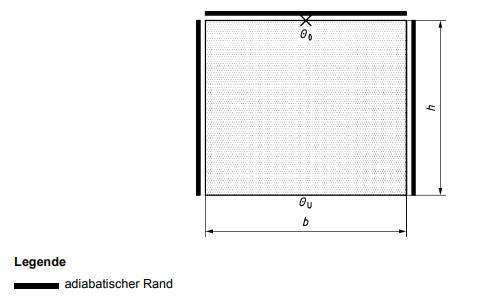
\includegraphics[width=0.8\textwidth]{din_example_1_plate.png}
  \caption{Geometry and boundary conditions considered in the validation example 1 \citep{DINEN1991_1_2}.}
\label{fig:din_example_1_plate}
\end{figure}

\begin{table}[htbp]
  \centering
  \caption{Material properties, and initial and boundary conditions for validation example 1.}
  \label{tab:din_example_1_description}
  \begin{tabular}{lccS[exponent-mode=engineering]}
  \multicolumn{3}{c}{Material Properties} & {\vphantom{\Big |}Effective value}\\
  \hline\hline
  \vphantom{\Big |}Conductivity & \(k\) & (\si{\watt\meter^{-1}\kelvin^{-1}}) & 1\\
  \vphantom{\Big |}Specific heat & \(c_p\) & (\si{\joule\per\kilo\gram\per\kelvin}) & 1\\
  \vphantom{\Big |}Density & \(\rho\) & (\si{\kilo\gram\per\meter^{3}}) & 1000\\
  \hline
  \multicolumn{3}{c}{Boundary Conditions\vphantom{\Big |}} & \\\hline
  \vphantom{\Big |}Dimensions & \(h\), \(b\) & (\si{\meter}) & 1\\
  \vphantom{\Big |}Heat convection coefficient & \(h_c\) & (\si{\watt\per\meter^2\per\kelvin}) & 1\\
  \hline
  \multicolumn{3}{c}{Initial Conditions\vphantom{\Big |}} & \\\hline
  \vphantom{\Big |}Ambient temperature & \(T_\infty\) & (\si{\celsius}) & 0\\
  \vphantom{\Big |}Temperature in cross-section & \(T_0\) & (\si{\celsius}) & 1000\\
  \hline
  \multicolumn{3}{c}{Reference value \vphantom{\Big |}} & \\\hline
  \vphantom{\Big |}Temperature \(T\) at point \(X\) & (\si{\celsius}) & \\
  \hline\hline
  \end{tabular}
\end{table}

\subsection{Results}

The numerical solutions obtained using FEM are presented in Table~\ref{tab:dim_example_1_comparison_table}, as well as, the reference values and the corresponding relative difference.
Figure~\ref{fig:dim_example_1_comparison} presents the same results in graphical form.
It can seen that that agreement between the numerical results and the reference solutions is very good, with relative error always smaller than \num{0.02}\%.
\cite{} recomends a relative difference \(\pm 1\%\) and an absolute difference \(\pm \SI{5}{\celsius}\).
Figure~\ref{fig:DIN_example_1_TRI3} shows different time instants of the numerical solution using TRI3 elements.
The evolution of the temperature field depicted seems reasonable given the description of the problem.

\begin{table}
  \caption{Reference and computed values for \(T_0\) concerning the validation example 1.}
  \label{tab:dim_example_1_comparison_table}
  \centering
  \begin{tabular}{SSc
      S[round-mode=places, round-precision=4]
      S[exponent-mode=scientific, round-mode=places, round-precision=2]}
   {Time (\si{\second})} & {\makecell{Reference value\\\(T_0\) (\si{\celsius})}} & \makecell{Element\\Type} & {\makecell{Computed value\\\(T'_0\) (\si{\celsius})}} & {\makecell{Relative difference\\\(\varepsilon\) (\(\%\))}} \\\hline\hline
   {\multirow{4}{*}{ 0 }} & {\multirow{4}{*}{ 1000.0 }} & TRI3  & 1000.0 & 0.0\\
   &  & TRI6 & 1000.0 & 0.0\\
   &  & QUAD4 & 1000.0 & 0.0\\
   &  & QUAD8 & 1000.0 & 0.0\\\hline
   {\multirow{4}{*}{ 60 }} & {\multirow{4}{*}{ 999.3 }} & TRI3  & 999.3436 & 0.004363054137904846\\
   &  & TRI6 & 999.2821 & 0.0017912538777084478\\
   &  & QUAD4 & 999.3434 & 0.004343040128091629\\
   &  & QUAD8 & 999.2821 & 0.0017912538777084478\\\hline
   {\multirow{4}{*}{ 300 }} & {\multirow{4}{*}{ 891.8 }} & TRI3  & 891.9305 & 0.014633325857826568\\
   &  & TRI6 & 891.7957 & 0.00048217089032785303\\
   &  & QUAD4 & 891.9308 & 0.01466696568737632\\
   &  & QUAD8 & 891.7957 & 0.00048217089032785303\\\hline
   {\multirow{4}{*}{ 600 }} & {\multirow{4}{*}{ 717.7 }} & TRI3  & 717.7402 & 0.005601226139043251\\
   &  & TRI6 & 717.6768 & 0.0032325484185715533\\
   &  & QUAD4 & 717.7403 & 0.005615159537411453\\
   &  & QUAD8 & 717.6768 & 0.0032325484185715533\\\hline
   {\multirow{4}{*}{ 900 }} & {\multirow{4}{*}{ 574.9 }} & TRI3  & 574.9004 & 6.957731779670875e-05\\
   &  & TRI6 & 574.8708 & 0.005079144198981763\\
   &  & QUAD4 & 574.9005 & 8.697164724094218e-05\\
   &  & QUAD8 & 574.8708 & 0.005079144198981763\\\hline
   {\multirow{4}{*}{ 1200 }} & {\multirow{4}{*}{ 460.4 }} & TRI3  & 460.4098 & 0.0021285838401479385\\
   &  & TRI6 & 460.4019 & 0.00041268462207529364\\
   &  & QUAD4 & 460.4098 & 0.0021285838401479385\\
   &  & QUAD8 & 460.4019 & 0.00041268462207529364\\\hline
   {\multirow{4}{*}{ 1500 }} & {\multirow{4}{*}{ 368.7 }} & TRI3  & 368.7175 & 0.004746406292374311\\
   &  & TRI6 & 368.7238 & 0.006455112557633379\\
   &  & QUAD4 & 368.7175 & 0.004746406292374311\\
   &  & QUAD8 & 368.7238 & 0.006455112557633379\\\hline
   {\multirow{4}{*}{ 1800 }} & {\multirow{4}{*}{ 295.3 }} & TRI3  & 295.286 & 0.004740941415513039\\
   &  & TRI6 & 295.3011 & 0.0003725025397927851\\
   &  & QUAD4 & 295.286 & 0.004740941415513039\\
   &  & QUAD8 & 295.3011 & 0.0003725025397927851\\
  \hline\hline
  \end{tabular}
\end{table}

% \begin{table}
%   \caption{Reference and computed values for \(T_0\) concerning the validation example 1 using TRI3 elements.}
%   \label{tab:dim_example_1_comparison_table}
%   \centering
%   \begin{tabular}{SS
%       S
%       S[exponent-mode=scientific, round-mode=places, round-precision=2]
%       c}
%   {Time (\si{\second})} & {\makecell{Reference value\\\(T_0\) (\si{\celsius})}} & {\makecell{Computed value\\\(T'_0\) (\si{\celsius})}} & {\makecell{Relative difference\\\(\varepsilon\) (\(\%\))}} & \makecell{Acceptable\\ difference \\according to \cite{}}\\\hline\hline
%   0 & 1000.0 & 1000.0 & 0.0 & \multirow{8}{*}{\makecell{\(\pm 1\%\)\\and\\\(\pm \SI{5.0}{\kelvin}\)}}\\
%   60 & 999.3 & 999.3436 & 0.004363054137904846 & \\
%   300 & 891.8 & 891.9305 & 0.014633325857826568 & \\
%   600 & 717.7 & 717.7402 & 0.005601226139043251 & \\
%   900 & 574.9 & 574.9004 & 6.957731779670875e-05 & \\
%   1200 & 460.4 & 460.4098 & 0.0021285838401479385 & \\
%   1500 & 368.7 & 368.7175 & 0.004746406292374311 & \\
%   1800 & 295.3 & 295.286 & 0.004740941415513039 & \\
%   \hline\hline
%   \end{tabular}
% \end{table}

\begin{figure}
   \centering
     \subfloat[][]{ 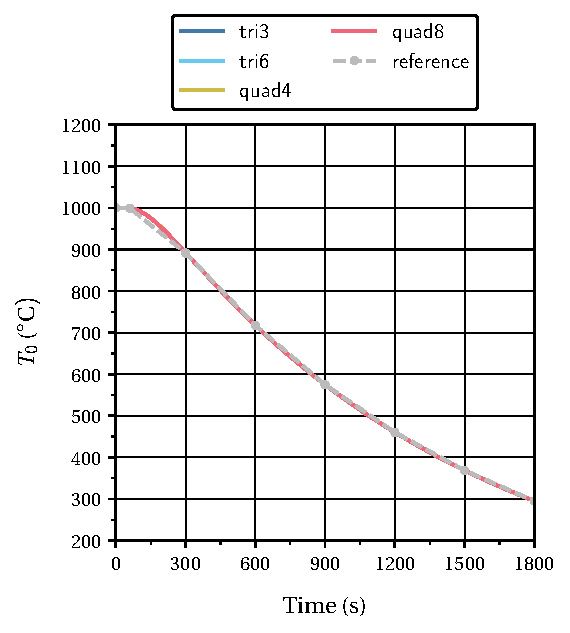
\includegraphics[width=0.5\columnwidth]{example_1_comparison_temp_ref_pt.pdf}
            \label{fig:example_1_comparison_temp_ref_pt}}
     \subfloat[][]{
    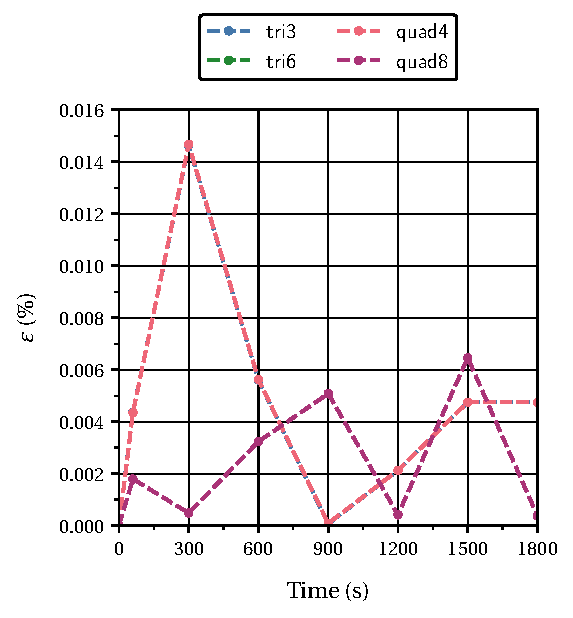
\includegraphics[width=0.5\columnwidth]{example_1_comparison_relative_error.pdf}
            \label{fig:example_1_comparison_relative_error}}
    \caption{Numerical results for the validation example 1. (a) Temperature values at \(X\) as a function of time. (b) Relative error in percentage as function of time.}
    \label{fig:dim_example_1_comparison}
\end{figure}

\begin{figure}
   \centering
     \subfloat[][$t=\SI{60}{\second}$]{ 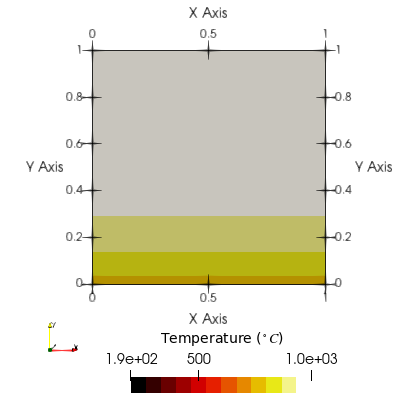
\includegraphics[width=0.5\columnwidth]{DIN_example_1_TRI3_t_60.png}
            \label{fig:DIN_example_1_TRI3_t_60}}
     \subfloat[][$t=\SI{600}{\second}$]{ 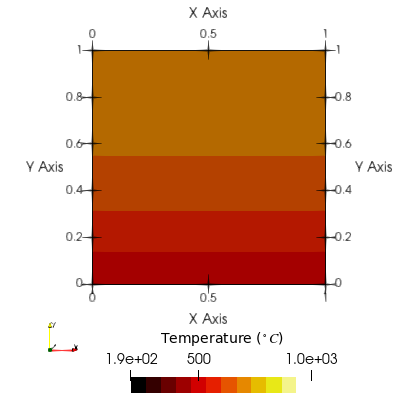
\includegraphics[width=0.5\columnwidth]{DIN_example_1_TRI3_t_600.png}
            \label{fig:DIN_example_1_TRI3_t_60}}\\
     \subfloat[][$t=\SI{1200}{\second}$]{
    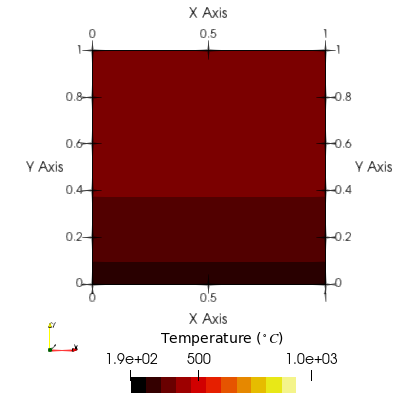
\includegraphics[width=0.5\columnwidth]{DIN_example_1_TRI3_t_1200.png}
            \label{fig:DIN_example_1_TRI3_t_60}}
     \subfloat[][$t=\SI{1800}{\second}$]{
    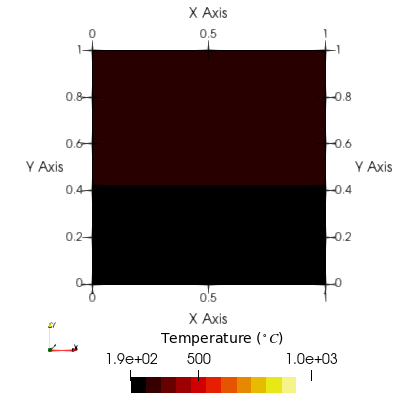
\includegraphics[width=0.5\columnwidth]{DIN_example_1_TRI3_t_1800.png}
            \label{fig:DIN_example_1_TRI3_t_60}}
    \caption{Numerical results regarding the evolution of the temperature distribution for the validation example 1 using a TRI3 mesh.}
    \label{fig:DIN_example_1_TRI3}
\end{figure}

\section{Validation example 2 - DIN EN 1991-1-2/NA:2010-12: Anhang CC - Prüfung und Validierung von Rechenprogramm für Brandschutznachweise mittels allgemeiner Rechenverfahren - Beispiel 2)}

\subsection{Description}

The geometry examined is a square plate with side length equal to \SI{0.2}{\meter}, as shown in Figure~\ref{fig:din_example_2_plate}.
There is heat transfer by convection along all the edges with a heat convection coefficient \(h_c\) equation to \SI{10}{\watt\meter^{-2}\kelvin^{-1}} and an environment temperature equal to \SI{1000}{\celsius} (see Equation~\ref{eq:heat_convection}).
Thre is also heat transfer through radition, with the emissivity \(\varepsilon_\text{res}\) equal to 0.8.
The initial temperature for the entire plate is \SI{0}{\celsius}.
Reference values for the temperature in the middle of the plate are supplied to determine performance.
The relevant properties of the material making up the plate are its conductivity \(k\), which follows a linear behavior (see Table~\ref{tab:din_example_2_description}), its specific heat \(c_p\), equal to \SI{1000}{\joule\kilo\gram^{-1}\kelvin^{-1}}, and its density \(\rho\), set equal to \SI{2400}{\kilo\gram\meter^{-3}}.
Table~\ref{tab:din_example_2_description} summarizes all the information regarding initial and boundary conditions, geometry and material properties.

\begin{figure}
  \centering
  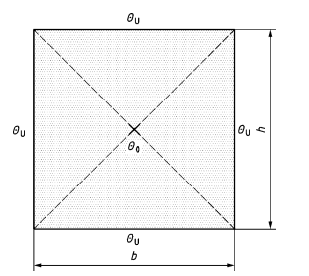
\includegraphics[width=0.55\textwidth]{din_example_2_plate.png}
  \caption{Geometry and boundary conditions considered in the validation example 2. \citep{DINEN1991_1_2}}
\label{fig:din_example_2_plate}
\end{figure}

\begin{table}
  \centering
  \caption{Material properties, and initial and boundary conditions for validation example 2.}
  \label{tab:din_example_2_description}
  \begin{tabular}{lccSS}
  \multicolumn{3}{c}{Material Properties} & \multicolumn{2}{c}{\vphantom{\Big |}Effective value}\\
  \hline\hline
  \multirow{4}{*}{\makecell{Conductivity \\(Linear behavior)}} &  \multirow{4}{*}{\(k\)} & \multirow{4}{*}{(\si{\watt\per\meter\per\kelvin})} & {\(T\)} & {\(\lambda(T)\)}\\\cline{4-5}
  & & & 0 & 1.5\\
  & & & 200 & 0.7\\
  & & & 1000 & 0.5\\
  \vphantom{\Big |} Specific heat & \(c_p\) & (\si{\joule\per\kilo\gram\per\kelvin}) & \multicolumn{2}{c}{1000}\\
  \vphantom{\Big |} Density & \(\rho\) & (\si{\kilo\gram\per\meter^{3}}) & \multicolumn{2}{c}{2400}\\
  \hline
  \multicolumn{3}{c}{Boundary Conditions\vphantom{\Big |}} & \\\hline
  \vphantom{\Big |}Dimensions & \(h\), \(b\) & (\si{\meter}) & \multicolumn{2}{c}{0.2}\\
  \vphantom{\Big |}Heat convection coefficient & \(h_c\) & (\si{\watt\per\meter^2\per\kelvin}) & \multicolumn{2}{c}{10}\\
  \vphantom{\Big |}Emissivity & \(\varepsilon_\text{res}\) &  & \multicolumn{2}{c}{0.8}\\
  \hline
  \multicolumn{3}{c}{Initial Conditions\vphantom{\Big |}} & \\\hline
  \vphantom{\Big |}Ambient temperature & \(T_\infty\) & (\si{\celsius}) & \multicolumn{2}{c}{1000}\\
  \vphantom{\Big |}Temperature in cross-section & \(T_0\) & (\si{\celsius}) & \multicolumn{2}{c}{0}\\
  \hline
  \multicolumn{3}{c}{Reference value \vphantom{\Big |}} & \\\hline
  \vphantom{\Big |}Temperature \(T_0\) in point \(X\) & & (\si{\celsius}) & \\
  \hline\hline
  \end{tabular}
\end{table}

\subsection{Results}

The numerical solutions obtained using FEM are presented in Table~\ref{tab:dim_example_2_comparison_table}, as well as, the reference values and the corresponding relative difference.
Figure~\ref{fig:dim_example_2_comparison} presents the same results in graphical form.
\cite{} recomends for \(t\leq \SI{60}{\minute}\) an absolute difference smaller than \(\pm \SI{5}{\celsius}\), and for \(t>\SI{60}{\minute}\), a relative difference smaller than \(\pm 2\%\).
It can be seen that that agreement between the numerical results and the reference solutions is acceptable.
For \(t\leq \SI{60}{\minute}\) the linear elements do not satisfy the recomendation set forth by \cite{}.
Otherwise the requirements are completly fullfiled.
Figure~\ref{fig:DIN_example_2_TRI3} shows different time instants of the numerical solution using TRI3 elements.
The evolution of the temperature field depicted seems reasonable given the description of the problem.

\begin{table}
  \caption{Reference and computed values for \(T_0\) concerning the validation example 2.}
  \label{tab:dim_example_2_comparison_table}
  \centering
  \begin{tabular}{SSc
      S[round-mode=places, round-precision=4]
      S[exponent-mode=scientific, round-mode=places, round-precision=2]}
   {Time (\si{\minute})} & {\makecell{Reference value\\\(T_0\) (\si{\celsius})}} & \makecell{Element\\Type} & {\makecell{Computed value\\\(T'_0\) (\si{\celsius})}} & {\makecell{Relative difference\\\(\varepsilon\) (\(\%\))}} \\\hline\hline
   {\multirow{4}{*}{ 0 }} & {\multirow{4}{*}{ 0.0 }} & TRI3  & 0.0 & 0.0\\
   &  & TRI6 & 0.0 & 0.0\\
   &  & QUAD4 & 0.0 & 0.0\\
   &  & QUAD8 & 0.0 & 0.0\\\hline
   {\multirow{4}{*}{ 30 }} & {\multirow{4}{*}{ 36.9 }} & TRI3  & 29.73116 & 19.427750677506772\\
   &  & TRI6 & 33.59058 & 8.96861788617885\\
   &  & QUAD4 & 30.42481 & 17.547940379403787\\
   &  & QUAD8 & 33.85025 & 8.26490514905148\\\hline
   {\multirow{4}{*}{ 60 }} & {\multirow{4}{*}{ 137.4 }} & TRI3  & 130.0251 & 5.367467248908294\\
   &  & TRI6 & 133.7875 & 2.629184861717621\\
   &  & QUAD4 & 131.0145 & 4.6473799126637605\\
   &  & QUAD8 & 133.8905 & 2.554221251819507\\\hline
   {\multirow{4}{*}{ 90 }} & {\multirow{4}{*}{ 244.6 }} & TRI3  & 240.0627 & 1.854987735077673\\
   &  & TRI6 & 242.8709 & 0.7069092395748112\\
   &  & QUAD4 & 240.404 & 1.7154538021259191\\
   &  & QUAD8 & 242.95 & 0.6745707277187268\\\hline
   {\multirow{4}{*}{ 120 }} & {\multirow{4}{*}{ 361.1 }} & TRI3  & 362.2362 & 0.3146496815286552\\
   &  & TRI6 & 363.4852 & 0.6605372472999163\\
   &  & QUAD4 & 361.9427 & 0.2333702575463803\\
   &  & QUAD8 & 363.5435 & 0.6766823594572062\\\hline
   {\multirow{4}{*}{ 150}} & {\multirow{4}{*}{ 466.2 }} & TRI3  & 470.0065 & 0.8164950664950725\\
   &  & TRI6 & 470.2503 & 0.8687902187902173\\
   &  & QUAD4 & 469.3439 & 0.674367224367231\\
   &  & QUAD8 & 470.2947 & 0.8783140283140259\\\hline
   {\multirow{4}{*}{ 180 }} & {\multirow{4}{*}{ 554.8 }} & TRI3  & 560.5277 & 1.0323900504686423\\
   &  & TRI6 & 560.1557 & 0.9653388608507697\\
   &  & QUAD4 & 559.6558 & 0.875234318673404\\
   &  & QUAD8 & 560.1907 & 0.9716474405191129\\
  \hline\hline
  \end{tabular}
\end{table}

% \begin{table}
%   \caption{Reference and computed values for \(T_0\) concerning the validation example 1 using TRI3 elements.}
%   \label{tab:dim_example_1_comparison_table}
%   \centering
%   \begin{tabular}{SS
%       S
%       S[exponent-mode=scientific, round-mode=places, round-precision=2]
%       c}
%   {Time (\si{\second})} & {\makecell{Reference value\\\(T_0\) (\si{\celsius})}} & {\makecell{Computed value\\\(T'_0\) (\si{\celsius})}} & {\makecell{Relative difference\\\(\varepsilon\) (\(\%\))}} & \makecell{Acceptable\\ difference \\according to \cite{}}\\\hline\hline
%   0 & 1000.0 & 1000.0 & 0.0 & \multirow{8}{*}{\makecell{\(\pm 1\%\)\\and\\\(\pm \SI{5.0}{\kelvin}\)}}\\
%   60 & 999.3 & 999.3436 & 0.004363054137904846 & \\
%   300 & 891.8 & 891.9305 & 0.014633325857826568 & \\
%   600 & 717.7 & 717.7402 & 0.005601226139043251 & \\
%   900 & 574.9 & 574.9004 & 6.957731779670875e-05 & \\
%   1200 & 460.4 & 460.4098 & 0.0021285838401479385 & \\
%   1500 & 368.7 & 368.7175 & 0.004746406292374311 & \\
%   1800 & 295.3 & 295.286 & 0.004740941415513039 & \\
%   \hline\hline
%   \end{tabular}
% \end{table}

\begin{figure}
   \centering
     \subfloat[][]{ 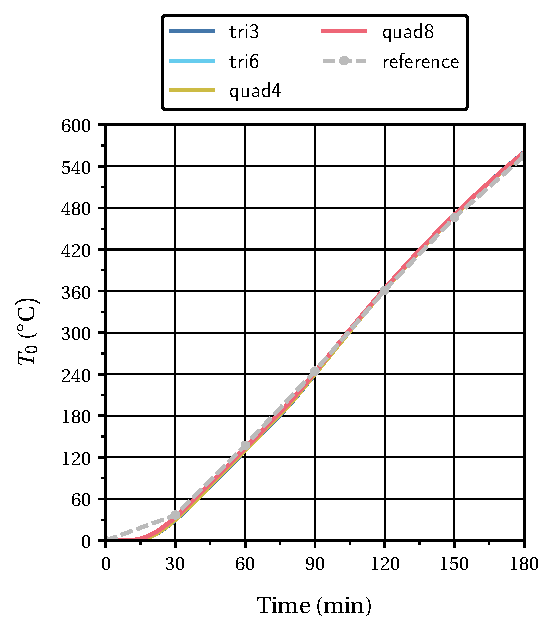
\includegraphics[width=0.5\columnwidth]{example_2_comparison_temp_ref_pt.pdf}
            \label{fig:example_2_comparison_temp_ref_pt}}
     \subfloat[][]{
    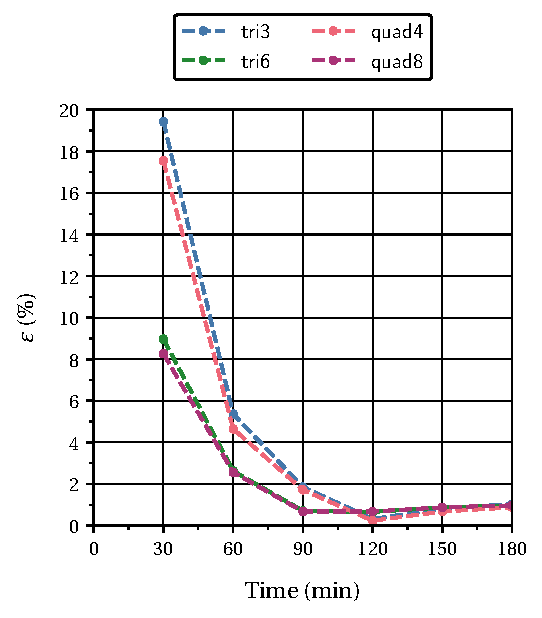
\includegraphics[width=0.5\columnwidth]{example_2_comparison_relative_error.pdf}
            \label{fig:example_2_comparison_relative_error}}
    \caption{Numerical results regarding the evolution of the temperature distribution for the validation example 2. (a) Temperature values at \(X\) as a function of time. (b) Relative error in percentage as function of time.}
    \label{fig:dim_example_2_comparison}
\end{figure}

\begin{figure}
   \centering
     \subfloat[][$t=\SI{30}{\minute}$]{ 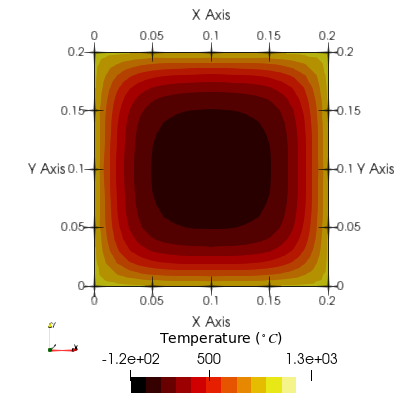
\includegraphics[width=0.5\columnwidth]{DIN_example_2_TRI3_t_30.png}
            \label{fig:DIN_example_2_TRI3_t_30}}
     \subfloat[][$t=\SI{90}{\minute}$]{ 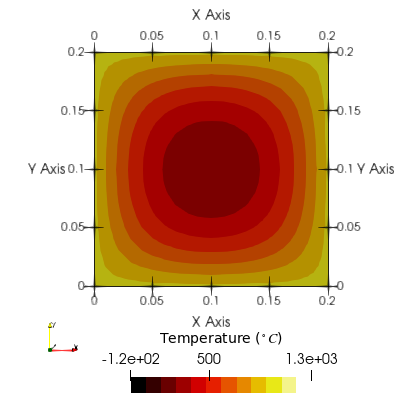
\includegraphics[width=0.5\columnwidth]{DIN_example_2_TRI3_t_90.png}
            \label{fig:DIN_example_2_TRI3_t_90}}\\
     \subfloat[][$t=\SI{120}{\minute}$]{
    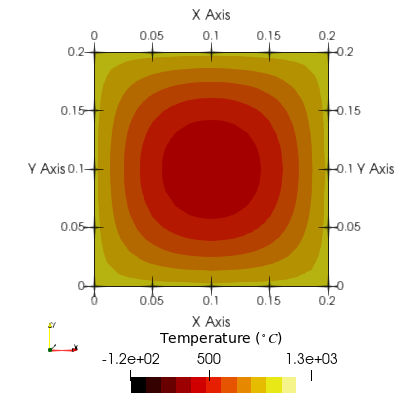
\includegraphics[width=0.5\columnwidth]{DIN_example_2_TRI3_t_120.png}
            \label{fig:DIN_example_2_TRI3_t_120}}
     \subfloat[][$t=\SI{180}{\minute}$]{
    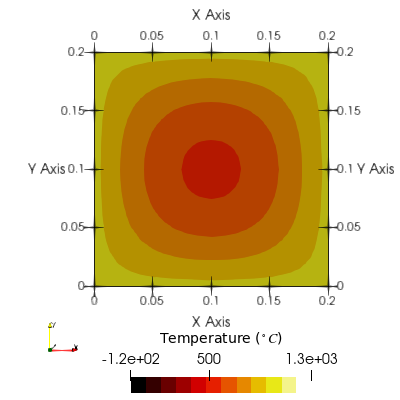
\includegraphics[width=0.5\columnwidth]{DIN_example_2_TRI3_t_180.png}
            \label{fig:DIN_example_2_TRI3_t_180}}
    \caption{Numerical results for the validation example 2 using a TRI3 mesh.}
    \label{fig:DIN_example_2_TRI3}
\end{figure}

\section{Validation example 3 - The Standard NAFEMS Benchmarks: linear thermo-elastic tests - Two dimensional heat transfer with convection}

\subsection{Description}

The geometry examined is a rectangular plate with width equal to \SI{0.6}{\meter} and length equal to \SI{1}{\meter}, as shown in Figure~\ref{fig:nafems_example_plate}.
A corresponding three-dimensional geometry is also considered with a thickness equal to \SI{1}{\meter}.
The boundary conditions considered are as follows: the left edge is assumed to be adiabatic.
At the lower edge the temperature is prescribed to be \SI{100}{\celsius} and along the upper and right edges there is heat transfer by convection and radiation.
The heat convection coefficient \(h\) is equal to \SI{70}{\watt\meter^{-2}\kelvin^{-1}}, and the ambient temperature is equal to \SI{0}{\celsius} (see Equation~\ref{eq:heat_convection}).
The initial temperature for the entire plate is \SI{0}{\celsius}.
The relevant properties of the material making up the plate are its conductivity \(k\), equal to \SI{52}{\watt\meter^{-1}\kelvin^{-1}}, its specific heat \(c_p\), equal to \SI{1}{\joule\kilo\gram^{-1}\kelvin^{-1}}, and its density \(\rho\), set equal to \SI{1}{\kilo\gram\meter^{-3}}.
Table~\ref{tab:nafems_example_description} summarizes all the information regarding initial and boundary conditions, geometry and material properties.
The expected temperature at E (see Figure~\ref{fig:nafems_example_plate}) is \SI{18.3}{\celsius}.


\begin{figure}
  \centering
  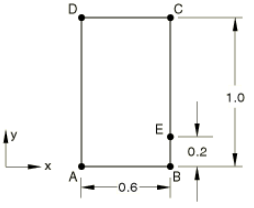
\includegraphics[width=0.55\textwidth]{nafems_example_plate.png}
  \caption{Geometry and boundary conditions considered in the validation example 3 \citep{NAFEMSbenchmarks}.}
\label{fig:nafems_example_plate}
\end{figure}

\begin{table}
  \centering
  \caption{Material properties, and initial and boundary conditions for validation example 3.}
  \label{tab:nafems_example_description}
  \begin{tabular}{lccS}
  \multicolumn{3}{c}{Material Properties} & {\vphantom{\Big |}Effective value}\\
  \hline\hline
  \vphantom{\Big |}Conductivity & \(k\) & (\si{\watt\meter^{-1}\kelvin^{-1}}) & 52\\
  \vphantom{\Big |}Specific heat & \(c_p\) & (\si{\joule\per\kilo\gram\per\kelvin}) & 1\\
  \vphantom{\Big |}Density & \(\rho\) & (\si{\kilo\gram\per\meter^{3}}) & 1\\
  \hline
  \multicolumn{3}{c}{Boundary Conditions\vphantom{\Big |}} & \\\hline
  \vphantom{\Big |}Dimension & \(h\) & (\si{\meter}) & 1\\
  \vphantom{\Big |}Dimension & \(b\) & (\si{\meter}) & 0.6\\
  \vphantom{\Big |}Thickness & \(t\) & (\si{\meter}) & 1\\
  Heat convection coefficient & \(h_c\) & (\si{\watt\per\meter^2\per\kelvin}) & 70\\
  \hline
  \multicolumn{3}{c}{Initial Conditions\vphantom{\Big |}} & \\\hline
  \vphantom{\Big |}Ambient temperature & \(T_\infty\) & (\si{\celsius}) & 100\\
  \vphantom{\Big |}Temperature in cross-section & \(T_0\) & (\si{\celsius}) & 0\\
  \hline
  \multicolumn{3}{c}{Reference value \vphantom{\Big |}} & \\\hline
  \vphantom{\Big |}Temperature \(T_0\) at point \(E\) & & (\si{\celsius}) & \\
  \hline\hline
  \end{tabular}
\end{table}

\subsection{Results}

The numerical solutions obtained using FEM are presented in Table~\ref{tab:nafems_example_comparison_table_2d} for two dimensions and in Table~\ref{tab:nafems_example_comparison_table_3d} for three-dimensions, as well as, the reference values and the corresponding relative difference.
It can be seen that that agreement between the numerical results and the reference solutions is acceptable.
It is below 1\% for all elements employed, except for the TETRA4 element.
There is no significant difference between the two integrators tested.
Figure~\ref{fig:NAFEMS_example_comparison} shows the temperature distribution obtained using TRI3 and TETRA10 elements, which is reasonable given the description of the problem.

\begin{table}
  \centering
  \caption{Reference and computed values for \(T_0\) concerning the validation example 3 in two-dimensions.}
\label{tab:nafems_example_comparison_table_2d}
  \begin{tabular}{c
  S[round-mode=places, round-precision=4]
  S[exponent-mode=scientific, round-mode=places, round-precision=2]}
  \vphantom{\Big |}Element & {\makecell{Temperature \(T_0\)\\at \(E\) \si{\celsius} } } & {\makecell{Relative\\ difference \(\varepsilon\) (\(\%\))}} \\
  \hline
  \multicolumn{3}{l}{\vphantom{\Big |}Alpha integrator (\(\rho=1\))}\\
  \hline
    TRI3 & 18.189045 & 0.6065573770491839\\
    TRI6 & 18.255251 & 0.24426229508198033\\
    QUAD4 & 18.228554 & 0.39016393442623263\\
    QUAD8 & 18.253191 & 0.2557377049180386\\
  \hline
  \multicolumn{3}{l}{\vphantom{\Big |}Quasi static integrator}\\
  \hline
    TRI3 & 18.189476 & 0.6038251366120318\\
    TRI6 & 18.254831 & 0.24699453551913246\\
    QUAD4 & 18.228132 & 0.39289617486338475\\
    QUAD8 & 18.253622 & 0.2535519125683169\\
    \hline\hline
  \end{tabular}
\end{table}

\begin{table}
  \centering
  \caption{Reference and computed values for \(T_0\) concerning the validation example 3 in three-dimensions.}
\label{tab:nafems_example_comparison_table_3d}
  \begin{tabular}{c
  S[round-mode=places, round-precision=4]
  S[exponent-mode=scientific, round-mode=places, round-precision=2]}
  \vphantom{\Big |}Element & {\makecell{Temperature \(T_0\)\\at \(E\) \si{\celsius} } } & {\makecell{Relative\\ difference \(\varepsilon\) (\(\%\))}} \\
  \hline
  \multicolumn{3}{l}{\vphantom{\Big |}Alpha integrator (\(\rho=1\))}\\
  \hline
    TETRA4 & 17.950129 & 1.9118633879781435\\
    TETRA10 & 18.255579 & 0.2427377049180318\\
  \hline
  \multicolumn{3}{l}{\vphantom{\Big |}Quasi static integrator}\\
  \hline
    TETRA4 & 17.949707 & 1.9141693989071074\\
    TETRA10 & 18.254831 & 0.2468251366120292\\
    \hline\hline
  \end{tabular}
\end{table}

\begin{figure}
   \centering
   \subfloat[][]{ 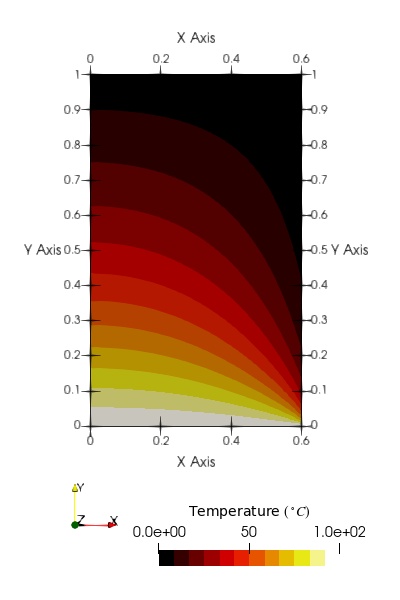
\includegraphics[width=0.5\columnwidth]{tri3_alpha.png}
   \label{fig:tri3_alpha}}
   \subfloat[][]{ 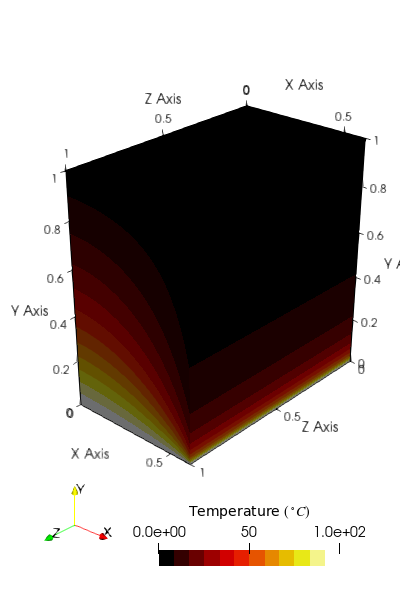
\includegraphics[width=0.5\columnwidth]{tetra10_alpha.png}
   \label{fig:tetra10_alpha}}
  \caption{Temperature distribution concercing the validation example 3: (a) in two-dimensions (TRI6) (b) in three-dimensions (TETRA4).}
\label{fig:NAFEMS_example_comparison}
\end{figure}


\chapter{Solution procedures for coupled fields}

An overview of solution techniques for coupled fields is provided in this chapter.
It comprises methods used to tackle a range of coupled field problems, including aeroelasticity, fluid-structure interaction, and thermomechanical coupling.
Its purpose is to aid in the selection of solution techniques for thermoplastic problems that are accurate, stable, efficient in terms of memory and computational effort, and simple to implement and subsequently expand to other couplings, such as the ones found in electro-thermomechanical problems.

\section{Context field elimination}

Field elimination achieves the solution of a coupled problem by eliminating the variables of the first field and introducing them into the second field.
This second field is then solved.

The decrease in the number of state variables is this procedure's key benefit.
It results in less complex equation systems that should be simpler to solve.
Other variables can also be chosen by the analyst so that they become the variables of interest.
In this manner, it is not necessary to retrieve the variables that were removed. \citep{felippa_staggered_1980}

On the other hand \cite{felippa_staggered_1980} cite as disadvantages
\begin{itemize}
  \item only possible for problems allowing explicit (and well-conditioned) variable eliminations;
  \item sparseness and symmetry attributes of matrices associated with the original coupled system can be adversely affected by the eliminations process; and
  \item available software modules for the isolated fields are not likely to be of much use for processing the reduced system.
\end{itemize}
The remainder of the chapter disregards these procedures, including in Section~\ref{} where the comparison of the different schemes is discussed.

\section{Monolithic}

Monolithic algorithms solve the coupled nonlinear multi-physics system simultaneously.
Implicit techniques are typically used to provide strong stability characteristics.
Likewise, the Newton-Raphson technique is frequently used to solve the nonlinear residual equations.
The effective solution of a large system of equations, including any potential nonlinearities or loss of symmetry, is a particular difficulty for monolithic algorithms.
Even the units chosen can contribute to the ill-conditioning of the system matrix.
Thus, a good preconditioning strategy is a key component of effective solvers for large-scale problems.

\subsection{Numerical considerations}

For the solution of a large system of equations, iterative methods are preferable to direct methods, in part, due to memory footprint considerations.
The Newton-Krylov methods such as GMRES and the BiCGStab are among the most commonly used in multi-physics problems \citep{hron_monolithic_2006}.
However, their use does not suffice for an efficient and robust solution procedure for a multi-physics problem.
In addition, the use of preconditioners alleviates the possible large condition numbers of the system matrix.
There are several preconditioning techniques for the solution of large systems of equations, e.g., ILU preconditioners, domain decomposition, including multigrid approaches; multilevel recursive Schur complements preconditioners (see \cite{smith_domain_2004} and \cite{chen_matrix_2005}).

\cite{heil_efficient_2004} is concerned with the fully coupled solution of large-displacement fluid-structure interaction problems by Newton's method.
They use block-triangular approximations of the Jacobian matrix, obtained by neglecting selected fluid-structure interaction blocks, and show that they provide suitable preconditioners for the solution of the linear systems with GMRES.
A Schur complement approximation for the Navier-Stokes block and multigrid approximations for the solution of the computationally most expensive operations is the basis for the efficient approximate implementation of the preconditioners.

\cite{hron_monolithic_2006} propose a method based on a fully implicit, monolithic formulation of the problem in the arbitrary Lagrangian-Eulerian framework  to solve the problem of fluid-structure interaction of an incompressible elastic object in laminar incompressible viscous flow
They utilize the standard geometric multigrid approach based on a hierarchy of grids obtained by successive regular refinement of a given coarse mesh.
The complete multigrid iteration is performed in the standard defect-correction setup with the V or F-type cycle.

\cite{tezduyar2006space} show how preconditioning techniques more sophisticated than diagonal preconditioning can be used in iterative solutions of the linear equation systems in fluid-structure interaction problems.

In \cite{gee_truly_2011}, the authors focus on the strong coupling fluid-structure interaction employing monolithic solution schemes.
Therein, a Newton-Krylov method is applied to the monolithic set of nonlinear equations.
They propose two preconditioners that apply algebraic multigrid techniques to the entire fluid-structure interaction system of equations.
As the first option, the authors employ a standard block Gauss-Seidel approach, where approximate inverses of the individual field blocks are based on an algebraic multigrid hierarchy tailored to the type of the underlying physical problem.
A monolithic coarsening scheme for the coupled system that uses prolongation and restriction projections constructed for the individual fields provides the basis for the second preconditioner.
The resulting nonsymmetric monolithic algebraic multigrid method involves coupling the fields on coarse approximations to the problem yielding significantly enhanced performance, claim the authors.

In the context of multi-physics problems, \cite{https://doi.org/10.1002/fld.2402} propose a fully coupled algebraic multilevel preconditioner for Newton-Krylov solution methods.
A set of multi-physics partial differential equation (PDE) applications attests its performance: a drift-diffusion approximation for semiconductor devices,
a low Mach number formulation for the simulation of coupled flow, transport, and non-equilibrium chemical reactions,
a low Mach number formulation for visco-resistive magnetohydrodynamics (MHD) systems.
An aggressive-coarsening graph-partitioning of the non-zero block structure of the Jacobian matrix provides the basis for the algebraic multilevel preconditioner.
Using a different approach \cite{badia_block_2014} employ a new family of recursive block LU preconditioners to solve the thermally coupled induction less magnetohydrodynamics problem equations, which model the flow of an electrically charged fluid under the influence of an external electromagnetic field with thermal coupling.

\cite{netz_high-order_2013} addresses a thermo-mechanically coupled problem of thermo-viscoelasticity at finite strains using a monolithic approach.
The authors solve the system of nonlinear algebraic equations obtained from the spatial (FEM) and temporal (diagonally-implicit Runge-Kutta methods) discretization of the problem monolithically.
They employ the Multilevel-Newton algorithm to obtain a high-order result in the space and the time domain.
The numerical concept is applied to a constitutive model of finite strain thermo-viscoelasticity.
\cite{rothe_monolithic_2015} also employ in the context of thermo-viscoelasticity, the multilevel Newton algorithm to solve the system of algebraic equations describing the discretized problem.

\cite{danowski_monolithic_2013} presents a monolithic solution scheme for thermo-structure interaction problem, using right preconditioning and a GMRES.
The preconditioner "sub-problem" is solved using a Richardson iteration scheme and a relaxed block Gauss-Seidel method, which uncouples the mechanical and thermal problems.
This procedure tackles each problem using an independent algebraic multigrid (AMG) preconditioner.
\cite{verdugo_unified_2016} also consider the procedure just mentioned, as well as a preconditioner based on a semi-implicit method for pressure-linked equations, extended to deal with an arbitrary number of fields.
This technique also results in uncoupled problems that can be solved with standard AMG.
They also introduce a more sophisticated preconditioner that enforces the coupling at all AMG levels, unlike the other two techniques, which resolve the coupling only at the finest level.
These techniques are applied successfully to three different coupled problems: thermo-structure interaction, fluid-structure interaction, and a complex model of the human lung.

\cite{mayr_hybrid_2020} propose a hybrid interface preconditioner for the monolithic solution of surface-coupled problems.
They combine physics-based block preconditioners with an additional additive Schwarz preconditioner, whose subdomains span across the interface on purpose.
This approach is motivated by the error assessment of physics-based block preconditioners, revealing an accumulation of the error at the coupling surface, despite their overall efficiency.

\newpage


\subsection{Usage examples}

\paragraph{Thermo-mechanical coupling}

In the following paragraph, a small overview of the literature is presented regarding the application of monolithic solvers to the thermo-mechanical coupled problem.
\cite{carter_finite_1989} suggests a monolithic approach to the thermoelastic problem at small strains.
The constitutive laws considered do not acknowledge the dependence of the mechanical properties on the temperature and are not deduced from a Helmholz energy function.
\cite{glaser_gekoppelte_1992} uses monolithic algorithms for the calculation of thin-walled structures using shell elements and an arc-length method for the TSI solution.
While all coupling terms were considered, only a simplified mechanical dissipation was included where the hardening power was neglected (according to \cite{danowski_computational_2014}).
\cite{ibrahimbegovic_covariant_2002} present a thermoplasticity covariant formulation within the framework of the principal axis methodology, which the authors claim, leads to a very efficient numerical implementation.
The paper contains several numerical simulations dealing with the fully coupled thermomechanical response at large viscoplastic strains, including strain localization and cyclic loading cases, to illustrate the performance of the proposed methodology.
The authors consider the von Mises thermoplasticity yield criterion and strain energy depending on logarithmic stretches, a hardening variable, and temperature.
A monolithic solver achieves the solution to the coupled problem, but no details about it are given.
\cite{danowski_computational_2014} proposes a volume-coupled TSI model based on the finite element method for the structural and thermal field.
Various temperature-dependent, isotropic, elastic, and elastoplastic material models for small and finite strains are employed, incorporating the effect of the highly elevated temperatures predominating in rocket nozzles, the practical application focused on in the Ph.D. thesis.
The author considers both monolithic and partitioned coupling algorithms to solve fully coupled thermomechanical systems.
Regarding the former,  a novel monolithic Newton-Krylov scheme with problem-specific block Gauss-Seidel preconditioner and algebraic multigrid methods is introduced.
Concerning the latter, loosely and strongly coupled partitioned schemes are examined, possibly including acceleration techniques, as, e.g., the Aitken \(\Delta^2\) method.
\cite{netz_high-order_2013} and \cite{rothe_monolithic_2015} both present monolithic approaches, based on the multilevel Newton method, for the solution of the thermo-mechanical problem.
In both contributions, thermo-visco-plastic materials are successfully analyzed.
Recently, \cite{felder_thermo-mechanically_2021} have presented a finite strain thermo-mechanically coupled two-surface damage-plasticity theory.
The authors obtain the solution for the three coupled fields, displacement, nonlocal damage variable, and temperature, employing an implicit and monolithic solution scheme.

The thermo-mechanical coupling has also been studied in the more specific domain of contact mechanics.
\cite{zavarise_real_1992} present one of the earliest contributions in this direction.
They propose a FEM formulation of frictionless contact, accounting for full thermo-elastic coupling.
The penalty method is used to enforce the non-penetration conditions.
Another contribution, \cite{hansen_jacobian-free_2011}, advances a standard mortar discretization with Lagrange multipliers to solve the small strain thermo-elasticity problem.
The authors consider the heat equation coupled to linear mechanics through a thermal expansion term in their formulation.
The solution approach is based on a preconditioned Jacobian-free Newton Krylov solution method, and the use case under analysis is a light water reactor nuclear fuel rod.
\cite{dittmann_isogeometric_2014} investigate thermomechanical mortar contact algorithms and their application to NURBS-based Isogeometric Analysis in the context of nonlinear elasticity.
Mortar methods are applied to both the mechanical and thermal fields to model frictional contact, the energy transfer between the surfaces, and frictional heating.
A monolithic approach is pursued in solving the nonlinear algebraic equations found after the discretization in time and space.
In the Ph.D. thesis by the same first author, \cite{dittmann_isogeometric_2017}, this approach is further pursued in multi-field contact problems.
More recently, \cite{seitz_computational_2018, seitz_computational_2019} tackles the numerical treatment of contact problems considering inelastic deformation and thermomechanical coupling.
It accounts for plastic spin, visco-plasticity, and thermo-plastic coupling, as well as temperature-dependent material parameters.
The authors also opt for a monolithic solver, although no further details are supplied.
See also, in the context of contact mechanics, \cite{oancea_finite_1997, pantuso_finite_2000, hueber_thermo-mechanical_2009, hesch_energy-momentum_2011, gitterle_dual_2012} and \cite{novascone_evaluation_2015}.

\paragraph{Others}

In the context of fluid-structure interaction, the monolithic approach seems to be more widely used than in thermo-mechanically coupled problems.
A few contributions in this domain using a monolith approach are \cite{blom_monolithical_1998, heil_efficient_2004, hubner_monolithic_2004, michler_monolithic_2004, zhangStudiesStrongCoupling2004, dettmer_computational_2006, hron_monolithic_2006, tezduyar2006space, kuttler_coupling_2010,gee_truly_2011, kloppel_fluidstructure_2011, mayr_temporal_2015} and \cite{mayr_hybrid_2020}.
The use of a monolithic approach can also be found in the domain of saturated soils (e.g., \cite{lewis_finite_1993}, \cite{borja_elastoplastic_1998}, \cite{jha_locally_2007}, \cite{white_stabilized_2008}).
Monolithic solvers are also used in the context of magnetohydrodynamics (e.g., \cite{SHADID20107649} and \cite{badia_block_2014}).



\section{Partitioned}

The following section presents the partitioned time-stepping algorithms.
For a detailed comparison with the monolithic approach and between themselves, see Section~\ref{sec:comparison_sol_methods}.

A field partition is a field-by-field decomposition of the space discretization.
Partitioning may be algebraic or differential.
In algebraic partitioning, the complete coupled system is spatially discretized first and then decomposed.
In differential partitioning, the decomposition is done first, and each field is then discretized separately.
Differential partitioning often leads to non-matched meshes, as is typical of fluid-structure interaction.
Algebraic partitioning was initially developed for matched meshes and substructuring \citep{felippa_partitioned_2001}.

The earliest contributions regarding the partitioned treatment of coupled systems emerged in the mid 1970s, involving structure-structure interactions and fluid-structure interactions (see e.g. \cite{belytschko_mesh_1976}, \cite{park_stabilization_1977}, \cite{belytschko_stability_1978}, \cite{hughes_implicit-explicit_1978} and \cite{belytschko_mixed_1979}).

% ``What are partitioned time-stepping algorithms?''

Given a complex system, there are usually many ways of partitioning it into subsystems or fields.
\cite{felippa_staggered_1980} provide a very pragmatic and helpful criterion to select the fields to be considered.
According to their definition, a field is characterized by computational considerations.
It is a segment of the overall problem for which a separable software module is either available or readily prepared if the interaction terms are suppressed.
As such, a partitioned approach to the solution of multi-physics problems employs field analyzers specific to each field separately stepped in time.
The coupling between the fields is achieved through proper communication between the individual components using prediction, substitution, and synchronization techniques.

% ``What is the difference between operator splits, fractional step, partitioned and staggered?''

Before moving on, it may be helpful to clear up the difference between partitioned schemes, staggered schemes, operator splits, and fractional-step methods.
The first is probably the most general term and includes the others.
Its definition has already been given.
A staggered scheme is a term most often used for the partitioned schemes where the solution concerning each field is sequential and obtained only once per time step as in the loosely coupled schemes to be introduced.
However, it may also include the strongly coupled schemes, as well.
An operator split is obtained through the decomposition of the fully coupled problem into subproblems.
The structure of the problem is the same, as well as the unknowns considered.
The only difference between the subproblems is the physical effects considered.
The equation terms concerning each physical effect must be divided exclusively and exhaustively between the subproblems.
Finally, according to \cite{armero_new_1992} staggered algorithms for coupled problems can be viewed as fractional steps methods, in the sense of \cite{holt_method_2012}, arising from an operator split of the coupled problem of evolution.

\subsection{Operator splits}

% ``What are operator splits?''
The most common operator splits into thermomechanical problems are the isothermic and adiabatic split.

\paragraph{Isothermic}

The isothermic split is perhaps the most straightforward and natural approach, as noted by \cite{argyris_natural_1981}, one of the earliest contributions on the topic.
The scheme achieves the solution of the thermo-mechanical problem, first solving the mechanical problem at a constant temperature, then a purely thermal phase is considered at a fixed configuration.

\paragraph{Adiabatic}

The adiabatic split is proposed in \cite{armero_new_1992}.
It consists of a first phase where constant entropy is enforced and a second phase of purely thermal conduction with a fixed reference.
In terms of implementation complexity, it is comparable to the isothermal split.
This is possible because the constant entropy phase can be cast as a mechanical phase, where the stiffness and the external force are adjusted as a function of an intermediate temperature.
This temperature is computed considering the strong form of the temperature evolution equation to retain the computational efficiency of the isothermal split, despite the momentum equation being enforced in its weak form.
The advantage of this split is that when used in a staggered scheme, it is unconditionally stable (see Section~\ref{sec:comparison_sol_methods}).


\subsection{Loosely vs. Strongly coupled schemes} \label{sec:loosely_strong_comp}

% ``What are the techniques used in partitioned schemes?''

According to \cite{felippa_partitioned_2001} there are several basic techniques associated with partitioned schemes (see Figure~\ref{fig:devices_of_partitioned_analysis_time_stepping}).
These are
\begin{itemize}
  \item preditction;
  \item substitution;
  \item interfield iteration;
  \item full step correction;
  \item lockstep advancing;
  \item midpoint correction;
  \item subcycling;
  \item augmentation.
\end{itemize}

\begin{figure}[htbp]
  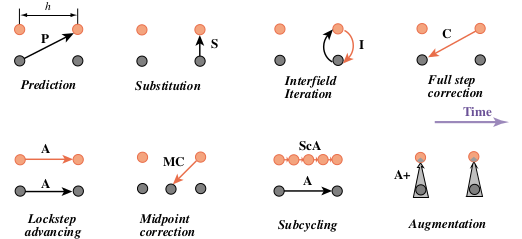
\includegraphics[width=\textwidth]{devices_of_partitioned_analysis_time_stepping.png}
  \caption{Devices of partitioned analysis time-stepping \citep{felippa_partitioned_2001}.}
\label{fig:devices_of_partitioned_analysis_time_stepping}
\end{figure}

Inter-field iterations are the primary criterion distinguishing loosely or one-way staggered coupled schemes and strongly or iterative staggered coupled schemes.
In the loosely coupled schemes, the integration algorithm proceeds sequentially, solving the problem in each field only once per time step.
On the other hand, for strongly coupled schemes, inter-field iterations are present, such that the problems are solved multiple times at the same time instant.
This inner loop is repeated until a given tolerance is reached for the unknowns in each field.

The remainder of the techniques listed will be mentioned and explained in the discussion below.

\subsection{Loosely coupled}



The solution for the fully coupled problem is found in loosely coupled schemes by solving each field sequentially.
For the thermomechanical problem, the two available schemes are the isothermal split (see e.g. \cite{simo_recent_1992}, \cite{agelet_de_saracibar_numerical_1998}) and the adiabatic split (see e.g. \cite{armero_new_1992} and \cite{armero_priori_1993}), as mentioned above.

According to \cite{felippa_partitioned_2001}, in linear problems, the first concern with partitioning is the degradation of time-stepping stability.
After the analyst has ensured stability, an accuracy analysis of the method should be performed.
In strongly nonlinear problems, such as fluid flow, stability and accuracy tend to be intertwined since numerical stability is harder to define.
As such, they are usually considered together in method design.
The expectation is for a method that operates well at a reasonable timestep.

\cite{felippa_partitioned_1988} present a detailed explanation about how to design from scratch a loosely coupled time-stepping algorithm applicable to linear systems of equations.
It includes implementation details, such as the choice of the predictor formula, and the design steps, from the formulation of the original field equations and temporal discretization to the stability and accuracy analysis.
Other contributions focused mainly on linear systems are \cite{neishlos_finite-element_1983}, \cite{zienkiewicz_unconditionally_1988} and \cite{combescure_numerical_2002},

Because the loosely coupled schemes are explicit, they are also often only conditionally stable.
The isothermic split is such an example \citep{armero_new_1992}.
On the other hand, the adiabatic split proposed in \cite{armero_new_1992} is unconditionally stable, despite being explicit.
\cite{farhat_unconditionally_1991} also propose a stable staggered scheme, achieved through semi-algebraic augmentation, which, however, is limited to linearized thermoelasticity.
In the context of coupled flow and geomechanics, \cite{kim_stability_2011-2} show that when the mechanical problem is solved first, the drained split combined with a backward Euler discretization is conditionally stable, and the undrained split is unconditionally stable when combined with midpoint rule.
When instead the flow problem is solved first, \cite{kim_stability_2011-1} show that the fixed-stress split is conditionally and the fixed-strain split is unconditionally stable for appropriate choices of the generalized midpoint rule.

Moreover, in the domain of fluid-structure interactions, it can be shown that staggered methods are inherently non-conservative.
As time progresses in the simulation, these schemes introduce parasitic energy at the boundary, which contributes to their poor numerical stability \citep{michler_relevance_2003}.
A further problem appears when solving these coupled physical problems, the so-called artificial added-mass effect, which leads to instability.
It manifests itself when a slender structure and fluid have similar densities, and the latter is modeled as an incompressible fluid \citep{causin_added-mass_2005, forster_robust_2007}.
It can even be shown that for every sequentially staggered scheme and spatial discretization of a problem, a mass ratio between the fluid and structural mass density can be found at which the coupled system becomes unstable \citep{forster_artificial_2007}.

Despite this, some contributions detail strategies allowing for the unconditional stability of these schemes.
As part of the development loop of commercial tire designs, \cite{gillard_efficient_2019} tackles the problem of tire hydroplaning.
The author presents a robust explicit coupling scheme that relies on rigorous control of the energy artificially introduced at the interface by the staggering process through a dynamic adaptation of the coupling time step size.
Regarding the artificial added-mass effect, \cite{farhat_robust_2010} demonstrates that even for fluid-structure applications with strong added mass effects, a carefully designed staggered and sub-iteration-free time-integrator can achieve numerical stability and robustness concerning the slenderness of the structure, as long as the fluid is justifiably modeled as a compressible medium.

Another technique available to improve the stability of loosely coupled schemes is (algebraic) augmentation.
It rests on the injection of one of the coupled equations into the other, after discretization in space, to 'soften' the system, either by reducing the large eigenvalues of the uncoupled stiff equation or by introducing some damping into it.
Some examples of this approach include \cite{park_stabilization_1977} and \cite{park_stabilization_1983}.

Yet another technique to ensure stability in the context of fluid-structure interactions is presented in \cite{fernandez_projection_2006}.
Stability is achieved employing a semi-implicit coupling scheme, splitting the added-mass, viscous effects, and geometrical/convective nonlinearities, through a Chorin-Temam projection scheme within the fluid.

Regarding accuracy, the loosely coupled schemes do not necessarily inherit the accuracy order of the schemes used in the integration of the separate fields, often being just of the first order in time \citep{farhat_provably_2006}.
However, some contributions detail approaches that are second-order time-accurate.
In the context of thermo-elasticity, \cite{armero_new_1992} show that a double-pass approach using the adiabatic split yields such a second-order accurate time-stepping algorithm.
A few approaches yield similar results in the domain of fluid-structure interaction (see \cite{piperno_explicitimplicit_1997}, \cite{farhat_provably_2006} and \cite{farhat_robust_2010}).
In any case, whatever the theoretical convergence order of the loosely coupled method, at a given time instant, the fully coupled discretized equations of the problem will never be exactly satisfied by the solutions found.
There is a lag between the fields considered, e.g., the mechanical and thermal fields in a thermomechanical problem.
In the context of strong coupling, this lag can be conceived as a numerical evaluation error.
Solving approximately the exact (i.e., aggregated) equations can be reinterpreted as exactly solving a set of approximate (i.e., segregated) equations.
Thus, one can construe loosely-coupled methods as solving a set of segregated equations instead of aggregated equations.
Accordingly, the incurred numerical evaluation error can be reinterpreted as a discretization error.
Loosely-coupled methods, therefore, satisfy conservation only in an asymptotic sense, i.e., for vanishing mesh width; this is a basic consistency requirement \citep{michler_efficient_2005}.

Prediction techniques can improve the order of the numerical evaluation error incurred by loosely-coupled partitioned methods.
For the sake of explanation, consider the thermo-mechanical problem being solved using the isothermic split.
When using predictors, instead of integrating the mechanical equations based on the structure's temperature in the previous time instant, a prediction can be used for the temperature of the structure boundary in the current time instant.
Such predictions are generally based on an extrapolation of the solution from the previous time step.
Prediction techniques improve the solution accuracy and stability of loosely-coupled methods \citep{piperno_explicitimplicit_1997, piperno_partitioned_2001, michler_efficient_2005, farhat_provably_2006}.

Another technique available to improve the accuracy of the loosely coupled methods is subcycling.
It involves solving each field's problems using different time steps since the fields present in a multi-physics problem often have different time scales.
In the context of aeroelasticity, \cite{piperno_partitioned_1995} claims that it can offer substantial computational advantages, including savings in the simulation CPU time because the structural field will be advanced fewer times.
\cite{farhat_high_1997} and \cite{piperno_explicitimplicit_1997} also argue for this technique along the same lines.

\paragraph{Usage examples}

The loosely coupled scheme has been used in the context of thermoelasticity \citep{argyris_natural_1981, armero_new_1992, johansson_thermoelastic_1993, miehe_entropic_1995, miehe_theory_1995, holzapfel_entropy_1996}, thermo-plasticity \citep{armero_new_1992, armero_priori_1993, simo_associative_1992, wriggers_coupled_1992, agelet_de_saracibar_numerical_1998, agelet_de_saracibar_formulation_1999} and thermo-viscoplasticity \citep{adam_numerical_2002, adam_numerical_2002-1}.

For examples in aeroelasticity see e.g., \cite{piperno_partitioned_1995, farhat_two_2000} and \cite{farhat_application_2003}, and in fluid-structure interaction more broadly see e.g. \cite{tezduyar2006space} and \cite{miller_loosely_2015}
Other applications include fluid-soil interaction analysis \citep{saetta_unconditionally_1992, armero_formulation_1999, mikelic_convergence_2013}.


\subsection{Strongly coupled}

In the strongly coupled scheme, inter-field iterations are performed until a given tolerance for the unknowns of each field is reached.
They converge to the solution of the monolithic scheme and are thus able to satisfy discrete versions of the coupled problem exactly \citep{forster_robust_2007, danowski_computational_2014}.
In principle, regarding thermomechanics, either the isothermal or the adiabatic slit can be used, but there seems to be no example of the latter.
In contrast to the staggered schemes, there is no problem of conditional stability, but the scheme may converge very slowly or not at all.
As an example coming from fluid-structure interactions, it has been shown that the number of coupling iterations increases when the time step decreases or when the structure becomes more flexible \citep{degroote_stability_2008}.
This can place a severe restriction on the use of these schemes.
Several acceleration techniques are available in the literature to speed up convergence.

A straightforward way to improve the convergence behavior of the strongly coupled schemes is using predictors, in contrast to the values found in the last step.
Thus, the initial guesses can be improved using well-chosen predictors \cite{michler_efficient_2005}.
Along these lines, \cite{erbts_accelerated_2012} employ polynomial prediction methods, and \cite{wendt_partitioned_2015} use a line extrapolation method to improve the first guess of the unknown and thus decrease the number of iterations needed to achieve convergence.

Another approach that is well established for series acceleration is the Aitken delta-squared process.
It uses previously computed values to obtain more accurate estimates for the unknown.
\cite{irons_version_1969} is an early contribution detailing this low-memory convergence acceleration scheme.
In the context of thermomechanics, \cite{danowski_computational_2014}, \cite{erbts_partitioned_2015} and \cite{wendt_partitioned_2015} use this technique, with the last authors also employing a quasi-Newton least squares method.
Some examples of contributions in the domain of fluid-structure interactions taking advantage of this approach are \cite{degroote_stability_2008}, \cite{kuttler_fixed-point_2008} and \cite{kuttler_vector_2009}.
The last authors also introduce a vector extrapolation approach that includes more than three previous values of the iteration scheme in the improved estimate.

The strongly coupled approach lends itself to an interpretation as a nonlinear block Jacobi or Gauss-Seidel scheme, whose convergence is conditional and at most linear \citep{matthies_strong_2003, joosten_analysis_2009}.
\cite{cervera_computational_1996} provides an in-depth analysis of block Jacobi and Gauss-Seidel schemes applied to coupled problems, including considerations regarding efficiency, complexity, and parallelization.
\cite{matthies_partitioned_2003, matthies_strong_2003} suggests a block-Newton method instead, with the Jacobian of the system being approximate by a finite difference method.
Under some assumptions on the subsystem solvers, this approach converges quadratically.
\cite{michler_interface_2005} propose a solution method based on the conjugation of sub-iterations via a Newton-Krylov method, which confines the GMRES acceleration to the interface degrees-of-freedom.
The latter renders storage requirements for the Krylov space and computational cost of the least-squares
problem low.
The nesting of Newton and GMRES iterations lends itself to the reuse of Krylov vectors in subsequent linear system solutions.
\cite{kuttler_vector_2009} claims that the approach proposed by the last authors should not be regarded as a Newton-based solver but as a Krylov-based vector extrapolation scheme

One can also improve the convergence speed of the strongly coupled scheme using reduced-order models to produce a more accurate first guess and thus decrease the number of iterations needed for the method to converge.
\cite{vierendeels_implicit_2007} presents a technique that uses the Jacobian from reduced-order models that are built up during the coupling iterations.
The reduced-order model is built for each step and approximates an arbitrary interface displacement fitting a linear regression to the previous displacement-stress points.
\cite{degroote_stability_2008} follows the same technique, coupling it with an Aitken delta-squared process.

\cite{blom_efficient_2017} proposes a manifold mapping technique to decrease the number of sub-iterations of a high-fidelity fluid-structure interaction model.
The idea is to perform many sub-iterations with a low-fidelity model instead of the high-fidelity flow and structure models.


\paragraph{Usage examples}

Regarding the use of strongly coupled schemes in the context of thermo-mechanics, there are a few contributions.
\cite{erbts_accelerated_2012} present results concerning thermo-elasticity at finite strains, \cite{netz_high-order_2013} concerning thermo-viscoelasticity, \cite{danowski_computational_2014} includes results on thermo-elasticity and thermo-elasto-plasticity.
In field of fluid-structure interaction, a few examples of the use of strongly coupled schemes are \cite{torii2006computer}, \cite{wall_strong_2007} and \cite{blom_efficient_2017}.
Including more than two fields, \cite{erbts_partitioned_2015} tackles electro-thermo-mechanical problems, as does \cite{wendt_partitioned_2015}, which also considers radiative heat transfer.
In \cite{lenarda_geometrical_2016}, the strongly coupled scheme is used to solve coupled hygro-thermo-mechanical problems in photovoltaic laminates.

\section{Comparison of solution techniques} \label{sec:comparison_sol_methods}

According to \cite{felippa_partitioned_1988}, the desirable properties of a time-stepping algorithm for solving coupled problems are:
\begin{itemize}
  \item enjoys unconditional stability;
  \item is highly accurate;
  \item is easy to implement;
  \item is not memory intensive;
  \item requires low CPU time;
  \item satisfies software modularity constraints.
  \end{itemize}
In the following, the time-stepping schemes presented above are compared with these criteria in mind.
The application in view is thermomechanics.

\paragraph{Stability}

Regarding stability, the loosely coupled using an isothermal split is conditionally stable \citep{armero_new_1992}.
Despite this, the limitation is not significant for metal plasticity, according to \cite{simo_associative_1992}.
However, examples where the scheme diverges, can be found in \cite{armero_new_1992}.
In this last contribution, the adiabatic split is introduced and shown to be unconditionally stable in the context of thermo-elasticity.
\cite{armero_priori_1993} show that these properties extend to thermo-plasticity.
The strongly coupled schemes are unconditionally stable because no critical time step leads to numerical instabilities in the results.
Despite this, the inner loop of the scheme may converge slowly or not at all \citep{matthies_strong_2003}.
It depends on the spectral radius of the matrices involved \citep{cervera_computational_1996}.
There are, however, acceleration techniques that can mitigate this problem, including predictors and Aitken \(\Delta^2\) methods (see Section~\ref{}).
\cite{danowski_computational_2014} presents a numerical example concerning an internal pressurized thick-walled cylinder, whose material is viscoplastic, for which the strongly coupled scheme employed diverged, despite the use of an Aitken method.
On the other hand, the monolithic scheme, as long as appropriately preconditioned, is unconditionally stable \citep{danowski_computational_2014}.

\paragraph{Accuracy}

Regarding accuracy, the solution found from the loosely coupled method will never exactly satisfy the fully coupled discretized equations of the problem.
There will be a time lag between the thermal and the mechanical field.
Loosely-coupled methods, therefore, satisfy conservation only in an asymptotic sense, i.e., for vanishing mesh width \citep{michler_efficient_2005}.
As long as it does not diverge, the monolithic and strongly coupled satisfy the coupled discretized equations exactly.

\paragraph{Ease of implementation}

The partitioned schemes are much easier to implement as most of them can work with the field analyzers as black boxes, concerning themselves only with communication between the solvers, initial guesses, and acceleration schemes using previously computed values.
The monolithic scheme requires the computation of the full stiffness matrix, including the mixed terms and appropriate preconditioning that varies widely with the specific multi-physics problem to be solved.

\paragraph{Memory requirements}

When it comes to memory requirements, the partitioned schemes often require only the diagonal blocks of the stiffness matrix found in the linearization process.
Previous values also need to be saved from one iteration to the next, increasing the memory cost for some acceleration techniques.
In contrast, the fully coupled monolithic scheme requires the full stiffness matrix of the coupled problem.

\paragraph{CPU time}

According to \cite{michler_efficient_2005}, solving a fluid-structure interaction problem with the same accuracy using a loosely and strongly coupled scheme, the latter is more efficient than the former.
For the same total number of iterations, the difference in the accuracy reached ranges from one to three orders of magnitude.
These results run counter to a claim in \cite{felippa_partitioned_2001}. However, this is not supported by any numerical results from the last authors.
In the numerical examples presented in \cite{danowski_computational_2014}, the monolithic solver is in most cases faster than a strongly coupled scheme employing an Aitken method for problems in thermomechanics.
The differences range from 120\% to 140\% in favor of the monolithic scheme.
Supporting evidence for these conclusions can also be found in \cite{novascone_evaluation_2015}.
The authors report  CPU time ratios between the strongly coupled and monolithic approaches, ranging from 0.635 to 3.75 on the magnitude of the coupling.

\paragraph{Software modularity}

The partitioned approaches can take full advantage of software, including closed source commercial solvers.
There is little to no software reuse for the monolithic approach, save for routines that solve linear systems and the like.

\paragraph{Conclusions}

Lastly, it may be helpful to reproduce the recommendations given in \cite{felippa_partitioned_2001} regarding the choice between partitioned and monolithic approaches.
According to the authors, the circumstances that favor the partitioned approach for tackling a coupled problem are a research environment with few delivery constraints, access to existing software, localized interaction effects (e.g., surface versus volume), and widespread spatial/temporal component characteristics.
The opposite circumstances:        commercial environment,        rigid deliverable timetable,        massive software development resources,        global interaction effects, and comparable length/time scales favors a monolithic approach.

Putting it all together, the most appropriate choice for the present use case is the strongly coupled schemes with appropriate acceleration techniques.
They can take advantage of already existing software, provide accurate results that agree with a monolithic approach, are not memory intensive, are easy to implement, and with the use of convergence acceleration techniques, are competitive from the computational efficiency standpoint.
The only drawback seems to be the possibility of divergence in the inner loop, stalling the progress of the simulation.

\begin{table}[htbp]
  \caption{Summary of the comparison between the FFT-Galerkin method.}
\label{tab:comparison_fft_galerkin_fem}
\small
  \setlength{\tabcolsep}{1pt}
  \centering
    \begin{tabular}{l ccc}
    & \multicolumn{2}{c}{Partitioned schemes} & \multirow{2}{*}{Monolithic} \\ \cline{2-3}
    & \vphantom{\Big |}Loosely coupled & Strongly coupled & \\
    \hline  \hline
    \vphantom{\Big |}Stability & \makecell[l]{Isothermic split:\\\ \textcolor{red!70!black}{conditionally stable}\\Adiabatic split:\\\ \textcolor{green!50!black}{unconditionally stable}} & \textcolor{green!50!black}{\makecell[c]{unconditionally\\stable\textsuperscript{*}}} & \textcolor{green!50!black}{\makecell[c]{unconditionally\\stable}}\\ \hline
    Accuracy & \textcolor{red!70!black}{\makecell[c]{Coupled discretized\\ equations not\\ satisfied exactly}} & \textcolor{green!50!black}{\makecell[c]{Coupled discretized\\ equations satisfied}} & \textcolor{green!50!black}{\makecell[c]{Coupled discretized\\ equations satisfied}} \\ \hline
    \makecell[l]{Ease of\\ implementation} & \multicolumn{2}{c}{\textcolor{green!50!black}{\makecell[c]{Only communication between field\\ analyzers stricly needed}}} & \makecell[l]{\textcolor{red!70!black}{Full coupling needed:}\\\ \textcolor{red!70!black}{\textbullet\ Computation of mixed}\\\ \textcolor{red!70!black}{terms of the Jacobian}\\\ \textcolor{red!70!black}{\textbullet\ Preconditioning needed}} \\ \hline
    \makecell[l]{Memory\\ requirements} & \multicolumn{2}{c}{\textcolor{green!50!black}{\makecell[c]{Only diagonal blocks of\\ the full stiffness matrix needed}}} & \textcolor{red!70!black}{Full stiffness matrix needed}\\ \hline
    \makecell[l]{Software modularity\\ constraints} & \multicolumn{2}{c}{\textcolor{green!50!black}{Full software modularity}} & \textcolor{red!70!black}{\makecell[c]{Poor or no\\ software modularity}}\\
  \hline\hline
  \multicolumn{4}{l}{\vphantom{\Huge |}\parbox{\textwidth}{\footnotesize{${}^*$ The inner loop of the strongly coupled scheme may converge very slowly or even diverge.}}}
  \end{tabular}
\end{table}

\newpage\null\thispagestyle{blank}\newpage

\chapter{Strongly coupled methods for coupled fields}

This chapter presents the most common strongly coupled/implicit methods employd for the solution of coupled field problems.
This presentation seeks to provide a literature overview of the available approaches.

% More thorough description of the chapter
Two main ways of realizing a strongly coupled approach to the solution of the coupled problem are presented.
The first focuses on fixed-point solvers, and acceleration/stabilization techniques for them.
The second deals with approaches based on the Newton-Raphson method, with the main problem tackled being an efficient and accurate approximation to the Jacobian.\jvc{In the end rewrite the description of the Chapter}

\section{Equations to be solved}

For the sake of clarity, the discretized equations of the thermo-mechanical problem at the next time instant, \(n+1\), which is the focus of the present work, are recovered here
\begin{gather}
    \mathbf M \ddot{\mathbf u}_{n+1} +\mathbf f_u^\text{\;int}(\bm \uptheta_{n+1}, \mathbf u_{n+1})-\mathbf f^\text{\;ext}_{u,n+1}=\mathbf 0, \label{eq:mech_problem} \\
    \mathbf C \dot{\bm \uptheta}_{n+1} +\mathbf f_\theta^\text{\;int}(\bm \uptheta_{n+1}, \mathbf u_{n+1})-\mathbf f^\text{\;ext}_{\theta,n+1}=\mathbf 0, \label{eq:therm_problem}
\end{gather}
where the complete definition of the material incremental discretized thermo-mechanical initial boundary value problem can be found in Chapter~\ref{chapter:thermo_mechanical_problem}.

As only partitioned approaches are being considered, the thermal and mechanical problems are solved separetely, i.e., Equation~\eqref{eq:mech_problem} is solved considering a fixed temperature and Equation~\eqref{eq:therm_problem} is solved assuming a fixed configuration.
To ease the discussion, consider the existence of two functions \(\pazocal U_{n+1}\) and \(\pazocal T_{n+1}\) that represent these solution procedures at timestep \(n+1\).
These so-called mechanical and thermal solvers satisfy
\begin{highlight}[innertopmargin=-5pt]
\begin{gather}
  \pazocal U\colon \mathscr K_{\theta, n+1}\to \mathscr K_{u,n+1},\quad \mathbf u = \pazocal U_{n+1}(\bm \uptheta),\\
  \pazocal T\colon \mathscr K_{u,n+1}\to \mathscr K_{\theta, n+1},\quad \bm \uptheta = \pazocal T_{n+1}(\mathbf u).
\end{gather}
\end{highlight}
See Chapter~\ref{} for detailed information on them.
In the following the subscripts on the solvers will be droped to avoid clutter.

The goal now is to consider functions, built using \(\pazocal U\) and \(\pazocal T\), whose roots are also the solutions to the thermo-mechanical problem (Equations~\eqref{eq:mech_problem} and \eqref{eq:therm_problem}).
Several examples can be provided.
The most appropriate for the current use-case are presented in what follows.
They can be found in \cite{uekermann_partitioned_2016} in the context of fluid-structure interaction.

Consider the residues defined as,
\begin{highlight}
\begin{equation} \label{eq:def_res_jacobi}
  \pazocal R_\text{J}\colon \mathscr K_{u,n+1}\times\mathscr K_{\theta,n+1} \to K_{u,n+1}\times\mathscr K_{\theta,n+1},\quad  \pazocal R_\text{J}(\mathbf u, \bm \uptheta) =
  \left\{\begin{array}{c}
  \mathbf u - \pazocal U(\bm \theta)\\
  \bm \uptheta - \pazocal T(\mathbf u)
  \end{array}\right\},
\end{equation}
\end{highlight}
and
\begin{highlight}
\begin{equation} \label{eq:def_res_gauss_seidel}
  \pazocal R_\text{GS}\colon \mathscr K_{\theta,n+1} \to\mathscr K_{\theta,n+1},\quad \pazocal R_\text{GS}(\bm \uptheta) =
  \bm \uptheta - \pazocal T\circ \pazocal U(\bm \uptheta),
\end{equation}
\end{highlight}
where the subscript "J" stands for Jacobi and the subscript "GS" for Gauss-Seidel.
The reason for this choice of subscripts is made clear in Section~\ref{}.


Since the methods described below for the solution of non-linear systems of equations apply to both functions \(\pazocal R_\mathrm{J}\) and \(\pazocal R_\mathrm{GS}\), a general function denoted as \(\pazocal R\), whose variable is \(\mathbf x\), is considered instead.
As already stated, the solution for the thermo-mechanical problem (Equations~\eqref{eq:mech_problem} and \eqref{eq:therm_problem}) can be abstracted as the solutions of
\begin{equation} \label{eq:abstract_residue_equation}
  \pazocal R(\mathbf x) = 0.
\end{equation}
To obtain simpler expressions in what follows, consider also the function
\begin{equation}
\pazocal S(\mathbf x) = \mathbf x - \pazocal R(\mathbf x),
\end{equation}
whose fixed point is the solution to the nonlinear system of equation in Equation~\eqref{eq:abstract_residue_equation}.

\jvc{Explain an difference vector/scalar}

\section{A classification scheme for iterative methods}
\jvc{Should we include more classification schemes? Classifiy by order also? And so on?}

Most methods available for the solution of systems of non-linear equations, such as the one in Equation~\eqref{eq:abstract_residue_equation}, are iterative methods.
They can be more precisely defined lettting \(\mathbf x^{k},\mathbf x^{k-1}, \ldots\), whose superscripts correspond to the loop of the iteration method, be approximants to \(\mathbf x_{n+1}\), whose subscript concerns the timestep

To better understand the landscape of available methods to solve nonlinear systems of equations, the iteration functions are classified according to the information they require following the classification scheme by \cite{traub_iterative_1982}.
Let \(\mathbf x^{k+1}\) be determined uniquely by information obtained at \(\mathbf x^{k}, \mathbf x^{k-1}, \ldots\), including the derivatives of any order of \(\pazocal R\).
Let the function that maps \(\mathbf x^{k}, \mathbf x^{k-1}, \ldots\) into \(\mathbf x^{k+1}\) be called \(\phi\).
Thus
\begin{highlight}
\begin{equation}
  \mathbf x^{k+1}=\phi\left(\mathbf x^{k},\pazocal R(\mathbf x^{k}), J_\pazocal{R}(\mathbf x^k), \dots\right),
\end{equation}
\end{highlight}
where \(\phi\) is called an iteration function, and \(J_\pazocal{R}\) is the Jacobian of \(\pazocal R\).
To prevent clutering \(\mathbf x^k\) will stand for its value as well as for the values of \(\pazocal R(\mathbf x^k)\), \(J_\pazocal{R}(\mathbf x^k)\) and further derivatives of higher order.
Then \(\phi\) is called a \textit{one-point iteration function}.
Most iteration functions which have been used for root-finding are one-point iteration functions. The most commonly known examples are the fixed point schemes and Newton's iteration method.

Next let \(\mathbf x^{k+1}\) be determined by new information at \(\mathbf x^{k}\) and reused information at \(\mathbf x^{k-1}, \ldots\).
Thus
\begin{highlight}
  \begin{equation}\label{eq:one_point_iteration_function_with_memory}
    \mathbf x^{k+1}=\phi\left(\mathbf x^{k} ; \mathbf x^{k-1}, \ldots\right) .
  \end{equation}
\end{highlight}
Then \(\phi\) is called a \textit{one-point iteration function with memory}.
The semicolon in Equation~\eqref{eq:one_point_iteration_function_with_memory} separates the point at which new data are used from the points at which old data are reused.
The best-known example of a one-point iteration function with memory is the secant iteration function.

Let \(\mathbf x^{k+1}\) be determined by new information at \(\mathbf x^{k}, \omega_{1}\left(\mathbf x^{k}\right), \ldots\), \(\omega_{i}\left(\mathbf x^{k}\right)\), \(i \geq 1\), where \(\omega_i\) denote operations on \(\mathbf x^k\).
No old information is reused.
Thus
\begin{highlight}
  \begin{equation}
    \mathbf x^{k+1}=\phi\left[\mathbf x^{k}, \omega_{1}\left(\mathbf x^{k}\right), \ldots, \omega_{i}\left(\mathbf x^{k}\right)\right].
  \end{equation}
\end{highlight}
\jvc{Include where each will be discussed.}
Then \(\phi\) is called a \textit{multipoint iterative function}.
Such methods include Aitken-Steffson method.

Finally, let \(\mathbf z_{j}\) represent the quantities \(\mathbf x^{j}, \omega_{1}\left(\mathbf x^{j}\right), \ldots, \omega_{i}\left(\mathbf x^{j}\right)\), \(i \geq 1\).
Let
\begin{highlight}
  \begin{equation} \label{eq:multipoint_iterative_function_with_memory}
  \mathbf x^{k+1}=\phi\left(\mathbf z^{k} ; \mathbf z^{k-1}, \dots \right) .
  \end{equation}
\end{highlight}
Then \(\phi\) is called a \textit{multipoint iterative function with memory}.
The semicolon in Equation~\eqref{eq:multipoint_iterative_function_with_memory} separates the points at which new data are used from the points at which old data are reused.
\jvc{What about Padé approximants?}

In the present work the criteria used for the choice of the iterative method used fit neatly into the ones provided by \cite{fang_two_2009} for problems in the context the electronic structure problems.
They are
\begin{enumerate}
  \item The dimensionality of the problem is large.
  \item \(\pazocal R(\mathbf x)\) is continuously differentiable, but the analytic form of its derivative is not readily available, or it is very expensive to compute.
  \item The cost of evaluating \(\pazocal R(\mathbf x)\) is computationally high.
  \item The problem is noisy. In other words, the evaluated function values of \(\pazocal R(\mathbf x)\) usually contain errors.
\end{enumerate}
\jvc{Justify why they fit neatly into our problem?}

As such the methods chosen must minimize the number of calls to \(\pazocal R\), as it is expensive to compute.
The amount of information saved from previous iterations must also be judiciously chosen as the dimensionality of the problem is large and this can lead to memory limitation.
Finally, the analytical for of the derivative \(\pazocal{R}\) is also not available, thus methods that use must be discarded.

\subsection{Predictor}

All iterative procedures considered solve the thermo-mechanical problem at a given timestep \(n+1\).
As the first value approximating \(\mathbf x_{n+1}\), one can employ the converged value of the previous timestep, \(\mathbf x_n\), however a very efficient way to increase the chances of stability and reduce computation time is to predict the optimal initial values at the beginning of every time step \citep{erbts_accelerated_2012, erbts_partitioned_2015, wendt_partitioned_2015}.
The prediction of the new solution by polynomial extrapolation is based on the converged solution of the last two or three timesteps.
This method is based on polynomial vector extrapolation which is quite easy to implement, and the extra computational input involved is negligible.

The maximum polynomial under consideration is of the order two, i.e., the new solution is extrapolated from the results from the last three time steps.
The predictors $\mathbf{x}^{*}$ for the order $p=1$ and $p=2$ polynomials read:
\begin{highlight}[innertopmargin=-5pt]
\begin{gather}
p=1:\quad \mathbf{x}_{n+1}^{*}=2 \mathbf{x}_{n}-\mathbf{x}_{n-1}, \\
p=2:\quad \mathbf{x}_{n+1}^{*}=3 \mathbf{x}_{n}-3 \mathbf{x}_{n-1}+\mathbf{x}_{n-2}.
\end{gather}
\end{highlight}

\subsection{Convergence criteria}

For an iterative method to be useful, there must be reasonable criteria to determine its convergence.
The iteration residual is defined as
\begin{equation}
\mathbf r^{k} = \pazocal R(\mathbf x^{k}),
\end{equation}
and if it is equal to zero then $\mathbf x$ is the solution to the system of nonlinear equations, i.e.,
\begin{equation} \label{eq:residual_definition}
\mathbf r = \pazocal R(\mathbf x) = \mathbf 0,
\end{equation}
and hence, a reasonable convergence measure for the iteration procedure.

The discrete  $L^{2}$-norm can be used to obtain a scalar representative of the vectorial residual \(\mathbf r^{k}=\left(r^{k,1}, \ldots, r^{k,m}\right)^{T}\) as
\begin{equation} \label{eq:absolute_residual_criterion}
\left\|\mathbf{r}^{k}\right\|_{L^{2}}=\sqrt{\sum_{i}\left(r^{k, i}\right)^{2}}.
\end{equation}

Directly using \eqref{eq:absolute_residual_criterion} yields an absolute convergence criterion
\begin{equation}
\left\|\boldsymbol{r} ^{k}\right\|_{L^{2}}<\epsilon_\mathrm{abs}.
\end{equation}
with $\epsilon_\mathrm{abs}>0$ as absolute convergence limit and convergence being obtained when the above condition renders valid.
However, since the absolute value of the $r^{k,i}$'s can change by orders of magnitude during one simulation, an absolute measure is not appropriate in all situations.
A relative measure solves this problem by setting the residual in relation with the current coupling iterate values as
\begin{equation}
\frac{\left\|\mathbf{r}^{k}\right\|_{L^{2}}}{\left\|\mathbf{x}^{k}\right\|_{L^{2}}}<\epsilon_\mathrm{rel}.
\end{equation}

Since a relative convergence measure can fail to work properly when the coupling iterate values are close to zero and rounding errors come into play, a combination of absolute and relative measure, where the absolute measure takes care of close to zero cases and the relative handles all other cases, is often a good choice.



\section{One-point iteration function}

\jvc{Write small description of the one-point iteration functions we are going to look at}

\subsection{Fixed-point approaches}

The application of the fixed-point method to obtain the roots of \(\pazocal R\) yields
\begin{equation}
  \mathbf x^{k+1} = \pazocal S(\mathbf x^k) = \mathbf x^k - \pazocal R(\mathbf x^k).
\end{equation}
If the particular functions defined on Equations~\eqref{eq:def_res_jacobi} and \eqref{eq:def_res_gauss_seidel} are used, one finds the  two basic Schwarz procedures commonly employed in strongly coupled solution procedures.
They are the additive or block Jacobi and the parallel Scharwz or Gauss-Seidel procedures.
The names originate from domain decomposition, and justify the subscripts employ in Equations~\eqref{eq:def_res_jacobi} and \eqref{eq:def_res_gauss_seidel}.

\subsubsection{Block Jacobi or Schwarz additive}

Applying the fixed-point approach to \(\pazocal R_\mathrm{J}\) (Equation~\eqref{eq:def_res_jacobi}), yields
\begin{align}
  \left\{\mathbf u^{k+1}, \bm\uptheta^{k+1}\right\}^T &= \pazocal S_\mathrm{J}(\mathbf u^k, \bm\uptheta^k)\\
   &= \left\{\mathbf u^k, \bm\uptheta^k\right\}^T - \pazocal R_\mathrm{J}(\mathbf u^k, \bm \uptheta^k),
\end{align}
This is the same as solving both the mechanical (Equation~\eqref{eq:mech_problem}) and the thermal problem (Equation~\eqref{eq:therm_problem}) in parallel.
Such a procedure is said to be Schwarz additive or block Jacobi, refering to the similarities with the procedure for the solution of linear systems of equations with the same name i.e.,
\begin{gather}
\mathbf u^{k+1} = \pazocal U(\bm \uptheta^k),\\
\bm \uptheta^{k+1} = \pazocal T(\mathbf u^k).
\end{gather}

Box~\ref{box:block_jacobi} shows the pseudo-code for the block Jacobi approach.

\begin{framedbox}[htb]
  \caption{Additive Schwarz procedure, also called block Jacobi, for one timestep.}
  \label{box:block_jacobi}
  \begin{center}
    \begin{minipage}{0.9\textwidth}
    \begin{enumerate}[(i)]
    \item \(\mathbf u^0 = \mathbf u_{n}\)
    \item \(\bm \uptheta^0 = \bm \uptheta_n\)
    \item Set fixed-point counter to zero: \(k=0\)
    \item Enter the fixed-point loop
    \begin{enumerate}[(1)]
      \item Solve the mechanical problem at fixed temeperature \(\bm \uptheta^k\): \(\mathbf u^{k+1} = \pazocal U(\bm \uptheta^k)\)
      \item Solve the thermal problem at a fixed configuration \(\mathbf u^k\): \(\bm \uptheta^{k+1} = \pazocal T(\mathbf u^k)\)
      \item If the desired accuracy has not been reached, update \(k=k+1\) and go to step (1).

    \end{enumerate}
    \end{enumerate}
    \end{minipage}
  \end{center}
\end{framedbox}

\subsubsection{Block Gauss-Seidel or Schwarz multiplicative}

Applying the fixed-point approach to \(\pazocal R_\mathrm{GS}\) (Equation~\eqref{eq:def_res_jacobi}), yields
\begin{equation}
  \bm\uptheta^{k+1} = \pazocal S_\mathrm{GS}(\bm\uptheta^k) =  \bm\uptheta^k - \pazocal R_\mathrm{GS}(\bm \uptheta^k).
\end{equation}
Thus, the fields are solved sequentially, where the output of the first solver is used as the input for the second solver.
This the solution procedure is said to be Scharwz multiplicative or block Gauss-Seidel.
\begin{gather}
\mathbf u^{k+1}  = \pazocal U(\bm \uptheta^k),\\
\bm \uptheta^{k+1} = \pazocal T(\mathbf u^{k+1}).
\end{gather}
One of the fields must be chosen as the first and this may be important \citep{joosten_analysis_2009}.
Here, the focus is on the sequence coinciding with the isothermic split, i.e., first the mechanical problem is solved at a fixed temeprature, and then the thermal problem is fixed at a fixed configuration.

Box~\ref{box:block_gauss_seidel} shows the pseudo-code for the block Gauss-Seidel approach.

\begin{framedbox}[htb]
  \caption{Multiplicative Schwarz procedure, also called block Gauss-Seidel, for one timestep.}
  \label{box:block_gauss_seidel}
  \begin{center}
    \begin{minipage}{0.9\textwidth}
    \begin{enumerate}[(i)]
    \item \(\mathbf u^0 = \mathbf u_{n}\)
    \item \(\bm \uptheta^0 = \bm \uptheta_n\)
      \item Set fixed-point counter to zero: \(k=0\)
    \item Enter the fixed-point loop
    \begin{enumerate}[(1)]
      \item Solve the mechanical problem at fixed temeperature \(\bm \uptheta^k\): \(\mathbf u^{k+1} = \pazocal U(\bm \uptheta^k)\)
      \item Solve the thermal problem at a fixed configuration \(\mathbf u^{k+1}\): \(\bm \uptheta^{k+1} = \pazocal T(\mathbf u^{k+1})\)
      \item If the desired accuracy has not been reached, update \(k=k+1\) and go to step (1).

    \end{enumerate}
    \end{enumerate}
    \end{minipage}
  \end{center}
\end{framedbox}

\subsection{Newton's method}

The Newton-Raphson or Newton scheme is a very popular iterative solution procedure for nonlinear systems of equations, which under appropriate conditions converges quadratically.
It can be applied to Equation~\eqref{eq:abstract_residue_equation} yielding
\begin{highlight}[innertopmargin=-5pt]
  \begin{gather}
    J_\pazocal{R}(\mathbf x^k)\Delta \mathbf x^k = - \pazocal R(\mathbf x^k), \label{eq:newton_system}\\
    \mathbf x^{k+1} = \mathbf x^k + \Delta \mathbf x^k. \label{eq:newton_iter}
  \end{gather}
\end{highlight}

In particular, using \(\pazocal R_\mathrm{GS}\), a few simplifications can be obtained. \jvc{Find the proper citations}
To ease the explanation, consider, a thermal residual operator $\pazocal{R}_{u}(\mathbf{u}, \bm{\uptheta})$ and a mechanical residual operator $\pazocal{R}_{\theta}(\mathbf{u}, \bm{\uptheta})$ defined to be the first and second components in the definition of \(\pazocal R_\mathrm{J}\) (Equation~\eqref{eq:def_res_gauss_seidel}).
Written in full
\begin{gather}
\pazocal{R}_{u}(\mathbf{u}, \bm{\uptheta})=\mathbf{u}-\pazocal{U}(\bm{\uptheta})=0, \\
\pazocal{R}_{\theta}(\mathbf{u}, \bm{\uptheta})=\bm{\uptheta}-\pazocal{T}(\mathbf{u})=0,
\end{gather}

From this, a block Newton iteration can be written as
\begin{equation} \label{eq:block_newton_raphson}
\left[\begin{array}{l}
J_{\pazocal{R}_{u}}\left(\mathbf u^k, \bm{\uptheta}^{k}\right) \\[7pt] J_{\pazocal{R}_{\theta}}\left(\mathbf{u}^{k}, \bm\uptheta^k\right)
\end{array}\right]
\left\{\begin{array}{c}\Delta \mathbf{u}^{k} \\ \Delta \bm{\uptheta}^{k}\end{array}\right\}
=-\left\{\begin{array}{l}\pazocal{R}_{u}\left(\mathbf{u}^{k}, \boldsymbol{\theta}^{k}\right) \\ \pazocal{R}_{\theta}\left(\mathbf{u}^{k}, \boldsymbol{\theta}^{k}\right)\end{array}\right\},
\end{equation}
and the update of the iteration variables reads
\begin{equation}
\left\{\begin{array}{l}
\mathbf{u}^{k+1} \\
\boldsymbol{\theta}^{k+1}
\end{array}\right\}=\left\{\begin{array}{l}
\mathbf{u}^{k} \\
\boldsymbol{\theta}^{k}
\end{array}\right\}+\left\{\begin{array}{c}
\Delta \mathbf{u}^{k} \\
\Delta \boldsymbol{\theta}^{k}
\end{array}\right\}.
\end{equation}


The system of equations in Equation~\eqref{} can be further symplified following \cite{degroote_development_2010} considering the defintions of the mechanical and thermal residuals and taking their derivatives.
It yields
\begin{equation}
\left[\begin{array}{cc}
\mathbf I & -J_{\pazocal{U}}\left(\bm{\uptheta}^{k}\right) \\[7pt] 
-J_{\pazocal{T}}\left(\mathbf{u}^{k}\right) & \mathbf I
\end{array}\right]
\left\{\begin{array}{c}\Delta \mathbf{u}^{k} \\ \Delta \bm{\uptheta}^{k}\end{array}\right\}
=-\left\{\begin{array}{l}\pazocal{R}_{u}\left(\mathbf{u}^{k}, \boldsymbol{\theta}^{k}\right) \\ \pazocal{R}_{\theta}\left(\mathbf{u}^{k}, \boldsymbol{\theta}^{k}\right)\end{array}\right\},
\end{equation}
Written in the form of a system of equations
\begin{align}
  \Delta \mathbf u^k - J_\pazocal{U}(\bm \uptheta^k) \Delta \bm\uptheta^k &= - \pazocal R_u(\mathbf u^k, \bm \uptheta^k),\\
  - J_\pazocal{T}(\mathbf u^k) \Delta \mathbf u^k + \Delta \bm\uptheta^k &= - \pazocal R_\theta(\mathbf u^k, \bm \uptheta^k).
\end{align}

Solving for \(\Delta \mathbf u^k\) and \(\Delta \bm \uptheta^k\), one finds
\begin{align}
  \left(\mathbf I + J_\pazocal{U}(\bm\uptheta^k)J_\pazocal{T}(\mathbf u^k)\right)\Delta \mathbf u^k &= - \pazocal R_u(\mathbf u^k, \bm \uptheta^k)+J_\pazocal{U}(\bm\uptheta^k)\pazocal R_\theta(\mathbf u^k, \bm\uptheta^k), \label{eq:explicit_eq_delta_u_newton}\\
  \left(\mathbf I + J_\pazocal{T}(\mathbf u^k)J_\pazocal{U}(\bm\uptheta^k)\right)\Delta \bm\uptheta^k &= - \pazocal R_\theta(\bm \uptheta^k, \mathbf u^k)+J_\pazocal{\theta}(\mathbf u^k)\pazocal R_u(\mathbf u^k, \bm\uptheta^k). \label{eq:explicit_eq_delta_theta_newton}
\end{align}
Thus, the Jacobians now needed are \(J_\pazocal{U}\) and \(J_\pazocal{T}\).
See Section~\ref{} for the practical application of this.

Every iteration of the Newton scheme involves at least one invocation of the thermal and mechanical solvers when computing $\pazocal{R}\left(\mathbf{u}^{k}\right)$ or both $\pazocal{R}_{u}\left(\mathbf{u}^{k}, \boldsymbol{\theta}^{k}\right)$ and $\pazocal{R}_{\theta}\left(\mathbf{u}^{k}, \boldsymbol{\theta}^{k}\right)$.

The critical point for black box equation coupling is how to obtain the derivative information in the Jacobi matrices.
Some of the methods presented in the following find approximations for the required Jacobian times vector products in different ways.

\subsubsection{Constant Underrelaxation}

One of the most straightforward ways to stabilize an iterative method is to use constant underrelaxation. \cite{gatzhammer_efficient_2014}
The relaxation is performed as follows
\begin{equation} \label{eq:constant_relaxation}
\mathbf x^{k+1}=(1-\omega) \mathbf x^{k}+\omega(\mathbf x^k - \pazocal R(\mathbf x^k))=\mathbf x^{k} -\omega \mathbf{r}^{k+1},
\end{equation}
where \(\omega\) is the relaxation factor chosen in the range \(0<\omega<1\), which corresponds to an underrelaxation, to achieve a stabilizing effect.

Applying to Equation~\eqref{eq:def_res_jacobi}
\begin{equation}
  \left\{\begin{array}{c}
    \mathbf u^{k+1}\\
    \bm \uptheta^{k+1}
  \end{array}\right\} =
  (1-\omega)
  \left\{\begin{array}{c}
    \mathbf u^{k}\\
    \bm \uptheta^{k}
  \end{array}\right\}
  + \omega
  \left\{\begin{array}{c}
    \pazocal U(\bm\uptheta^k)\\
    \pazocal T(\mathbf u^k)
  \end{array}\right\}
\end{equation}
Applying to Equation~\eqref{eq:def_res_gauss_seidel}
\begin{equation}
  \bm\uptheta^{k+1} = (1-\omega)\bm\uptheta^k + \omega \pazocal T\left(\pazocal U(\bm \uptheta^k)\right).
\end{equation}


Constant underrelaxation works well if \(\omega\) is close to 1 , but leads to a slow convergence if \(\omega\) has to be chosen close to 0.
Thus, the constant underrelaxation method leads to unmanageable computational costs for severe instabilities.
The optimal \(\omega\) is not necessary the largest stable one \citet{gatzhammer_efficient_2014} and has to be set empirically.
In what follows, alternative methods are discussed, which try to decrease the number of iterations necessary while still keeping stability.

\begin{framedbox}[htb]
  \caption{Constant underrelaxation applied to the block Gauss-Seidel scheme.}
  \label{box:constant_underrelaxation}
  \begin{center}
    \begin{minipage}{0.9\textwidth}
    \begin{enumerate}[(i)]
    \item \(\bm\uptheta^0 = \bm\uptheta_{n+1}^p\)
    \item Set fixed-point counter to zero: \(k=0\)
    \item Enter the fixed-point loop
    \begin{enumerate}[(1)]
      \item Solve the mechanical problem at fixed temeperature \(\bm \uptheta^k\): \(\mathbf u^{k+1} = \pazocal U(\bm \uptheta^k)\)
      \item Solve the thermal problem at a fixed configuration \(\mathbf u^{k+1}\): \(\bm \uptheta^{k+1} = \pazocal T(\mathbf u^{k+1})\)
      \item Compute \(\bm \uptheta^{k+1}\) using constant relaxation (Equation~\eqref{eq:constant_relaxation})
      \item If the desired accuracy has not been reached, update \(k=k+1\) and go to step (1).
    \end{enumerate}
    \end{enumerate}
    \end{minipage}
  \end{center}
\end{framedbox}

\section{One-point iteration function with memory}

\jvc{Description of the methods}

\subsubsection{Aitken relaxation}

\citep{irons_version_1969, kuttler_fixed-point_2008, joosten_analysis_2009, kuttler_vector_2009, erbts_partitioned_2015, wendt_partitioned_2015}


The so-called Aitken \(\Delta^2\) relaxation method was introduced by \cite{irons_version_1969}, as a modified Aitken \(\Delta^2\) that doesn't require the computation of the function twice per iteration as in the original method.
In the one-dimensional case, this method resembles the secant method applied to the fixed point problem, which can be used to solve nonlinear equations without differentiation.
Calling it an Aitken method is perhaps a misnommer since in the Aitken-Steffson method, the values of the function are computed twice per iteration.
It is more closely related to secant methods, where values from previous iterations are reused.
This version of Aitken's \(\Delta^2\) method provides a dynamic underrelaxation, which can be used to improve the convergence/stability properties of coupling algorithm.

In the one-dimensional case
Assume that \(f\) is the function whose fixed point is sought.
The linear interpolation between two points already known of the function, \((a, f(a))\) and \((b, f(b)\) is
\begin{equation}
  y = \frac{f(b)-f(a)}{b-a}(x-a) - f(a).
\end{equation}
The fixed point of this approximation is
\begin{equation}
  c = \frac{f(b)-f(a)}{b-a}(x-c) - f(a).
\end{equation}
Thus, after rearranging,
\begin{equation}
c=\frac{a f(b)- b f(a)}{\left(a-f(a)\right)-\left(b-f(b)\right)}
\end{equation}
This can be rewritten as
\begin{equation}
c=\left(1-\omega_{b}\right) f(b)+\omega_{b} b \quad \text { with } \omega_{b}=\frac{f(b)-f(a)}{\left(a-f(a)\right)-\left(b-f(b)\right)}
\end{equation}

The difference \(f(b)-f(a)\) is computationally inconvenient.\jvc{Why?}
Anticipating the next iteration step,
\begin{equation}
d=\left(1-\omega_{c}\right) f(c)+\omega_{c} c \quad \text { with } \omega_{c}=\frac{f(c)-f(b)}{\left(b-f(b)\right)-\left(c-f(c)\right)}
\end{equation}
a convenient expression for updating the relaxation factor may be found, i.e.
\begin{equation}
\omega_{c}=\omega_{c}+\left(\omega_{b}-1\right) \frac{c-f(c)}{\left(b-f(b)\right)-\left(c-f(c)\right)}.
\end{equation}

Now, for the vector case, the next step is to work out the solution to the current iteration from the outcome of the previous iteration $\mathbf{x}^{(k)}$ plus a new increment $\Delta \mathbf{x}^{(k)}$
\begin{equation}
\mathbf{x}^{(k+1)}=\mathbf{x}^{(k)}+\Delta \mathbf{x}^{(k)}.
\end{equation}
The increment reads
\begin{equation}
\Delta \mathbf{x}^{(k)}=\omega^{(k)}\left(\pazocal S(\mathbf{x}^{(k)})-\mathbf{x}^{(k)}\right)=-\omega^{(k)} \mathbf r^{(k)}.
\end{equation}
with $\omega^{(k)}$ being the relaxation coefficient.
This coefficient is updated in every iteration cycle as a function of two previous residuals
\begin{highlight}
  \begin{equation}
    \omega^{(k)}=-\omega^{(k-1)} \frac{\left(\mathbf{r}^{(k)}-\mathbf{r}^{(k-1)}\right)^{\mathrm{T}} \mathbf{r}^{(k-1)}}{\left(\mathbf{r}^{(k)}-\mathbf{r}^{(k-1)}\right)^{2}}.
  \end{equation}
\end{highlight}
Comparing with Equations~\eqref{eq:newton_system} and \eqref{eq:newton_iter}, \(\omega^{(k)}\) can be, in a sense, regarded as an approximation to the inverse of the Jacobian.
Dynamic relaxation is also easy to implement and the additional computational input is acceptable, since only inner vector products have to be performed.

\subsection{Broyden's method and Broyden's family}

In quasi-Newton methods the Jacobian is updated in each iteration using a rank-one update.
Standard quasi-Newton methods require the updated \(J_{k+1}\) to satisfy the following secant condition
\begin{equation} \label{eq:secant_condition}
J_\pazocal{R}^{k+1} \Delta \mathbf x^{k}=\Delta \pazocal R^{k},
\end{equation}
where \(\Delta \pazocal R^{k}\equiv \pazocal R\left(\mathbf x^{k+1}\right)-\pazocal R\left(\mathbf x^ {k}\right)\).
Furthermore, another common requirement is the following so-called no-change condition
\begin{equation} \label{eq:no_change_condition}
J_\pazocal R^{k+1} \mathbf q=J_\pazocal R^{k} \mathbf q \quad \forall \mathbf q \text { such that } \mathbf q^{\mathrm{T}} \Delta \mathbf x^{k}=0,
\end{equation}
which stipulates that there be no new information from \(J_\pazocal R^{k}\) to \(J_\pazocal R^{k+1}\) along any direction \(\mathbf q\) orthogonal to \(\Delta \mathbf x^{k}\).

\cite{broyden} developed a method satisfying both secant condition (Equation~\eqref{eq:secant_condition}) and the no-change condition (Equation~\eqref{eq:no_change_condition}).
By simply imposing these conditions he arrived at the update formula
\begin{highlight}
\begin{equation} \label{eq:good_update_broyden}
J_{\pazocal R}^{k+1}=J_{\pazocal R}^{k}+\left(\Delta \pazocal R^{k}-J_{\pazocal R}^{k} \Delta \mathbf x^{k}\right) \frac{\Delta {\mathbf x^{k}}^{\mathrm{T}}}{\Delta {\mathbf x^{k}}^{\mathrm{T}} \Delta \mathbf x^{k}}.
\end{equation}
\end{highlight}

Matrix \(J_\pazocal R^{k+1}\) in Equation~\eqref{eq:good_update_broyden} is the unique matrix satisfying both conditions \eqref{eq:secant_condition} and \eqref{eq:no_change_condition}.
The Broyden update can also be obtained by minimizing \(E\left(J_\pazocal R^{k+1}\right)=\left\|J_\pazocal R^{k+1}-J_\pazocal R^{k}\right\|_{F}^{2}\) with respect to terms of \(J_\pazocal R^{k+1}\), subject to the secant condition \eqref{eq:secant_condition}.

It may seem at first that Broyden's first method can be expensive since computing the quasi-Newton step \(\Delta \mathbf x^{k}\) requires solving a linear system at each iteration.
However, note that, typically, the approximate Jacobian is a small rank modification of a diagonal matrix (or a matrix that is easy to invert); hence, the cost to obtain this solution is actually not too high as long as the number of steps is not too large.

An alternative is Broyden's second method that approximates the inverse Jacobian instead of the Jacobian itself.
\(G_\pazocal R^{k}\) is used to denote the estimated inverse Jacobian at the \(k\) th iteration.
The secant condition (Equation~\eqref{eq:secant_condition}) now reads
\begin{equation} \label{eq:inverse_secant_cond}
G_\pazocal R^{k+1} \Delta \pazocal R^{k}=\Delta \mathbf x^{k}
\end{equation}
By minimizing \(E\left(G_\pazocal R^{k+1}\right)=\left\|G_\pazocal R^{k+1}-G_\pazocal R^{k}\right\|_{F}^{2}\) with respect to \(G_\pazocal R^{k+1}\) subject to Equation~\eqref{eq:inverse_secant_cond}, the following update formula is found for the inverse Jacobian
\begin{highlight}
  \begin{equation} \label{eq:bad_update_broyden}
  G_\pazocal R^{k+1}=G_\pazocal R^{k}+\left(\Delta \mathbf x_{k}-G_\pazocal R^{k} \Delta \pazocal R^{k}\right) \frac{\Delta {\pazocal R^{k}}^{\mathrm{T}}}{\Delta {\pazocal R^{k}}^{\mathrm{T}} \Delta \pazocal R^{k}}
  \end{equation}
\end{highlight}
which is also the only update satisfying both the secant condition (Equation~\eqref{eq:inverse_secant_cond}) and the no-change condition for the inverse Jacobian
\begin{equation}
  G_\pazocal R^{k} \mathbf q=G_\pazocal R^{k+1} \mathbf q \quad \forall \mathbf q \text { such that } \mathbf q^{\mathrm{T}} \Delta \pazocal R^{k}=0.
\end{equation}
The update formula in Equation~\eqref{eq:good_update_broyden} can also be obtained in terms of \(G_\pazocal R^{k} \equiv {J_\pazocal R^{k}}^{-1}\) by applying the Sherman-Morrison formula
\begin{equation}
G_\pazocal R^{k+1}=G_\pazocal R^{k}+\left(\Delta \mathbf x^{k}-G_\pazocal R^{k} \Delta \pazocal R^{k}\right) \frac{\Delta {\mathbf x^{k}}^{\mathrm{T}} G_\pazocal R^{k}}{\Delta {\mathbf x^{k}}^{\mathrm{T}} G_\pazocal R^{k} \Delta \pazocal R^{k}}
\end{equation}
This shows, as was explained earlier, that to solve the Jacobian system associated with Broyden's first approach can be reduced to a set of update operations that are not more costly than those required by the second update.
Note, however, that the above formula requires the inverse of the initial Jacobian.

From Equation~\eqref{eq:good_update_broyden} and Equation~\eqref{eq:bad_update_broyden} it is possible to define Broyden's family of updates, in which an update formula takes the general form
\begin{equation}
G_\pazocal R^{k+1}=G_\pazocal R^{k}+\left(\Delta \mathbf x^{k}-G_\pazocal R^{k} \Delta \pazocal R^{k}\right) \mathbf v_{k}^{\mathrm{T}}
\end{equation}
where \(\mathbf v_{k}^{\mathrm{T}} \Delta \pazocal R^{k}=1\) so that the secant condition \eqref{eq:secant_condition} holds.
Note that the secant condition \eqref{eq:inverse_secant_cond} is equivalent to condition \eqref{eq:secant_condition}.
The pseudo-code of Broyden's two methods is given in Box~\ref{}.
Some authors called Broyden's first method as Broyden's good update, and Broyden's second method as Broyden's bad update.
These are two particular members in Broyden's family.

% \subsubsection{Steepest Descent Relaxation}
%
% In [97], a steepest descent based relaxation method is investigated. The goal is to find an optimal value \(\omega_{k}\) for every iteration \(k\) and to use it in the relaxation (2.112). A convex scalar merit function \(\phi(\boldsymbol{s})\) is assumed to exist, to be minimal at the solution \(\boldsymbol{s}^{n+1}\), and to be sufficiently smooth. This merit function is not defined in [97], only its derivative is used within the algorithm which is defined to be the coupling iteration residual
% \[
% \phi^{\prime}\left(\boldsymbol{s}_{k}\right):=\boldsymbol{r}_{k+1},
% \]
%
% such that \(\phi^{\prime}\left(s^{n+1}\right)=\mathbf{0}\). Using the merit function, an optimal relaxation factor can be found by
% \[
% \omega_{k}=\underset{\omega}{\arg \min } \phi\left(\boldsymbol{s}_{k}+\omega \boldsymbol{r}_{k+1}\right)
% \]
% and a sufficient condition for the optimal \(\omega_{k}\) is given by
% \[
% \frac{d \phi}{d \omega_{k}}=\left(\phi^{\prime}\left(\boldsymbol{s}_{k}+\omega_{k} \boldsymbol{r}_{k+1}\right)\right)^{T} \boldsymbol{r}_{k+1} \stackrel{!}{=} \mathbf{0} .
% \]
% An approximation for the optimal relaxation factor can be obtained from a truncated Taylor expansion of its first derivative
% \[
% \phi^{\prime}\left(\boldsymbol{s}_{k}+\omega_{k} \boldsymbol{r}_{k+1}\right) \approx \underbrace{\phi^{\prime}\left(\boldsymbol{s}_{k}\right)}_{=\boldsymbol{r}_{k+1}}+\omega_{k} \phi^{\prime \prime}\left(\boldsymbol{s}_{k}\right) \boldsymbol{r}_{k+1},
% \]
% where \(\phi^{\prime \prime}\left(s_{k}\right)\) is the symmetric matrix of second order partial derivatives of \(\phi\left(s_{k}\right)\) or the Jacobian of \(r_{k}\) with respect to \(s_{k}{ }^{5}\) Transposing (2.133) and multiplying it from the right with \(r_{k+1}\), the optimal relaxation factor can be obtained by
% \[
% \omega_{k}=-\frac{\left(\boldsymbol{r}_{k+1}\right)^{T} \boldsymbol{r}^{k+1}}{\left(\boldsymbol{r}^{k+1}\right)^{T} J_{\boldsymbol{r}_{k}}(\boldsymbol{s}) \boldsymbol{r}_{k+1}} .
% \]
% The remaining problem is how to determine the interface Jacobian \(J_{r_{k}}(s)\), since it is not accessible when black box solvers are used. Two approximations for the matrix vector product \(J_{\boldsymbol{r}_{k}}(s) \boldsymbol{r}_{k+1}\) are proposed in [97]. The first approximation is obtained by using a finite difference approach as
% \[
% J_{\boldsymbol{r}_{k}}(\boldsymbol{s}) \boldsymbol{y} \approx \frac{\boldsymbol{S} \circ \boldsymbol{F}\left(\boldsymbol{s}_{k}+\delta \boldsymbol{y}\right)-\boldsymbol{s}_{k}-\delta \boldsymbol{y}-\boldsymbol{r}_{k+1}}{\delta},
% \]
% with
% \[
% \delta=\frac{\lambda\left(\lambda+\left\|\boldsymbol{s}_{k}\right\|_{L_{2}}\right)}{\left\|\boldsymbol{r}_{k+1}\right\|_{L_{2}}}
% \]
% and \(\lambda\) chosen small enough \({ }^{6}\). The evaluation of (2.135) needs one more call of fluid and structure solvers per coupling iteration. To decrease the computational costs for the extra evaluation, it is proposed to reduce the accuracy within the field solvers. The second approximation uses approximated fluid derivatives and exact structure derivatives, which are not available for black box coupling and, thus, this alternative is not considered here.

\subsection{Multi-secant methods}

The multi-secant methods provide an approximation to the Jacobian in Equation~\eqref{} or Equation~\eqref{} using information from previous iterations.
The following exposition follows closely \cite{fang_two_2009}.

\subsubsection{Generalized Broyden}

A generalized Broyden's method with a flexible rank of update on the inverse Jacobian, satisfying a set of \(m\) secant equations
\begin{equation} \label{eq:multi_secant_eqs}
  G_\pazocal R^{k} \Delta \pazocal R^{i}=\Delta \mathbf x^{i} \quad \text { for } i=k-m, \ldots, k-1
\end{equation}
where it is assumed \(\Delta \pazocal R^{k-m}, \ldots, \Delta \pazocal R^{k-1}\) are linearly independent and \(m \leqslant n\) can also be described.
Aggregating Equations~\eqref{eq:multi_secant_eqs} in matrix form, they can be rewriten it as
\begin{equation} \label{eq:multi_secant_eqs_mat}
  G_\pazocal R^{k} \mathscr{R}^{k}=\mathscr{X}^{k}.
\end{equation}
where
\begin{equation}
\mathscr{R}^{k}=\left[\Delta \pazocal R^{k-m} \cdots \Delta \pazocal R^{k-1}\right], \quad \mathscr{X}^{k}=\left[\Delta \mathbf x^{k-m} \cdots \Delta \mathbf x^{k-1}\right] \in \mathbb{R}^{n \times m}
\end{equation}
The no-change condition corresponding to \eqref{eq:no_change_condition} is
\begin{equation}
  \left(G_\pazocal R^{k}-G_\pazocal R^{k-m}\right) \mathbf q=0
\end{equation}
for all \(\mathbf q\) orthogonal to the subspace spanned by \(\Delta \pazocal R^{k-m}, \ldots, \Delta \pazocal R^{k-1}\), the columns of \(\mathscr{R}^{k}\).
In the end, this yields
\begin{equation}
  G_\pazocal R^{k}=G_\pazocal R^{k-m}+\left(\mathscr{X}^{k}-G_\pazocal R^{k-m} \mathscr{R}^{k}\right)\left({\mathscr{R}^{k}}^{\mathrm{T}} \mathscr{R}^{k}\right)^{-1} {\mathscr{R}^{k}}^{\mathrm{T}}
\end{equation}
a rank-\(m\) update formula.
Note that \(\operatorname{rank}\left(\mathscr{R}^{k}\right)=m\).
The update formula for \(\mathbf x^{k+1}\) is
\begin{align}
\mathbf x^{k+1} &=\mathbf x^{k}-G_\pazocal R^{k} \pazocal R^{k} \\
&=\mathbf x^{k}-G_\pazocal R^{k-m} \pazocal R^{k}-\left(\mathscr{X}^{k}-G_\pazocal R^{k-m} \mathscr{R}^{k}\right)\left({\mathscr{R}^{k}}^{\mathrm{T}} \mathscr{R}^{k}\right)^{-1} {\mathscr{R}^{k}}^{\mathrm{T}} \pazocal R^{k} \\
&=\mathbf x^{k}-G_\pazocal R^{k-m} \pazocal R^{k}-\left(\mathscr{X}^{k}-G_\pazocal R^{k-m} \mathscr{R}^{k}\right) \gamma_{k} \label{eq:update_gen_broyden_ls}
\end{align}
where the column vector \(\gamma_{k}\) is obtained by solving the normal equations \(\left({\mathscr{R}^{k}}^{\mathrm{T}} \mathscr{R}^{k}\right) \gamma_{k}={\mathscr{R}^{k}}^{\mathrm{T}} \pazocal R^{k}\), which is equivalent to solving the least squares problem
\begin{equation}
  \min _{\gamma}\left\|\mathscr{R}^{k} \gamma-\pazocal R^{k}\right\|_{2}
\end{equation}
Note that in Equation~\eqref{eq:update_gen_broyden_ls}, if \(\mathscr{R}^{k}\) is square and of full rank, then for any \(G_\pazocal R^{k-m}\),
\begin{equation}
  \mathbf x^{k+1}=\mathbf x^{k}-\mathscr{X}^{k} {\mathscr{R}^{k}}^{-1} \pazocal R^{k}
\end{equation}
the same form as that in the standard secant method.

\subsubsection{Anderson mixing}

The Anderson mixing scheme [5] takes the latest \(m\) steps into account, with the goal of obtain a better approximation to \(\mathbf x_{n+1}\) without evaluating \(\pazocal R\) again.
Consider
\begin{align}
  \bar{\mathbf x}^{k}=\mathbf x^{k}-\sum_{i=k-m}^{k-1} \gamma_{i}^{k} \Delta \mathbf x^{i}=\mathbf x_{k}-\mathscr{X}^{k} \gamma^{k}, \label{eq:anderson_x_bar}\\
  \bar{\pazocal R}^{k}=\pazocal R^{k}-\sum_{i=k-m}^{k-1} \gamma_{i}^{k} \Delta \pazocal R^{i}=\pazocal R^{k}-\mathscr{R}^{k} \gamma^{k} \label{eq:anderson_r_bar},
\end{align}
where \(\Delta \mathbf x^{i}=\mathbf x^{i+1}-\mathbf x^{i}\) and \(\Delta \pazocal R^{i}=\pazocal R^{i+1}-\pazocal R^{i}\), \(\mathscr{X}^{k}=\left[\Delta \mathbf x^{k-m} \cdots \Delta \mathbf x^{k-1}\right]\), \(\mathscr{R}^{k}=\left[\Delta \pazocal R^{k-m} \cdots \Delta \pazocal R^{k-1}\right]\), and \(\gamma^{k}=\left[\gamma_{k-m}^{k} \cdots \gamma_{k-1}^{k}\right]^{\mathrm{T}}\).
Expressing the equations in the form \(\bar{\mathbf x}^{k}=\sum_{j=k-m}^{k} w_{j} \mathbf x^{j}\) and \(\bar{\pazocal R}^{k}=\sum_{j=k-m}^{k} w_{j} \pazocal R^{j}\), it is found that \(\sum_{j=k-m}^{k} w_{j}=1\).
In other words, \(\bar{\mathbf x}_{k}\) and \(\bar{\pazocal R}_{k}\) are weighted averages of \(\mathbf x_{k-m}, \ldots, \mathbf x_{k}\) and \(\pazocal R^{k-m}, \ldots, \pazocal R^{k}\), respectively.
The arguments \(\gamma^{k}=\left[\gamma_{k-m}^{k} \cdots \gamma_{k-1}^{(k)}\right]^{\mathrm{T}}\) are determined by minimizing
\begin{equation}
E\left(\gamma^{k}\right)=\left\langle\bar{\pazocal R}^{k}, \bar{\pazocal R}^{k}\right\rangle=\left\|\pazocal R^{k}-\mathscr{R}^{k} \gamma_{k}\right\|_{2}^{2}
\end{equation}
whose solution can, but should not in practice, be obtained by solving the normal equations
\begin{equation}
\left({\mathscr{R}^{k}}^{\mathrm{T}} \mathscr{R}^{k}\right) \gamma^{k}={\mathscr{R}^{k}}^{\mathrm{T}} \pazocal R^{k}. \label{eq:normal_eqs_anderson}
\end{equation}
Combining Equations~\eqref{eq:anderson_x_bar}, \eqref{eq:anderson_r_bar}, and \eqref{eq:normal_eqs_anderson}, one obtains
\begin{align}
\mathbf x^{k+1} &=\bar{\mathbf x}^{k}+\beta \bar{\pazocal R}^{k} \\
&=\mathbf x^{k}+\beta \pazocal R^{k}-\left(\mathscr{X}^{k}+\beta \mathscr{R}^{k}\right) \gamma^{k} \\
&=\mathbf x^{k}+\beta \pazocal R^{k}-\left(\mathscr{X}^{k}+\beta \mathscr{R}^{k}\right)\left({\mathscr{R}^{k}}^{\mathrm{T}} \mathscr{R}^{k}\right)^{-1} {\mathscr{R}^{k}}^{\mathrm{T}} \pazocal R^{k} \label{eq:update_anderson_mixing}
\end{align}
where \(\beta\) is the preset mixing parameter and \({\mathscr{R}^{k}}^{\mathrm{T}} \mathscr{R}^{k}\) is assumed to be nonsingular.
In particular, if no previous iterate is taken into account (i.e. \(m=0\) ), then Equation~\eqref{eq:update_anderson_mixing} reads
\begin{equation}
  \mathbf x^{k+1}=\mathbf x^{k}+\beta \pazocal R^{k}
\end{equation}
This scheme is referred to as simple mixing and underrelaxation if \(0<\beta<1\) (see Section~\ref{}).
The update formula \eqref{eq:update_anderson_mixing} is the same as \eqref{eq:update_gen_broyden_ls} by setting \(G_\pazocal R^{k-m}=-\beta \mathbf I\).
In this respect Anderson mixing implicitly forms an approximate inverse Jacobian \(G_\pazocal R^{k}\) that minimizes \(\left\|G_\pazocal R^{k}+\beta \mathbf I\right\|_{F}\) subject to \eqref{eq:multi_secant_eqs_mat}.
In the context of mixing, generalized Broyden's second method is equivalent to Anderson mixing. This equivalence relation was shown by Eyert [9].
Note that if \(\mathscr{R}^{k}\) is square and nonsingular, then Equation~\eqref{eq:update_anderson_mixing} matches the formula of the standard secant method.

\subsubsection{Generalized Broyden's family}

Now we can write down the generalized Broyden family, in which an update algorithm is in the form
\begin{equation} \label{eq:inv_jacob_gen_broyden}
G_\pazocal R^{k}=G_\pazocal R^{k-m}+\left(\mathscr{X}^{k}-G_\pazocal R^{k-m} \mathscr{R}^{k}\right) {V^{k}}^{\mathrm{T}}
\end{equation}
where \({V^{k}}^{\mathrm{T}} \mathscr{R}^{k}=I\) so that the secant condition \(G_\pazocal R^{k} \mathscr{R}^{k}=\mathscr{X}^{k}\) holds.
The two optimal choices of \({V^k}^T = {M^k}^{-1}{N^k}^T\) are
\begin{equation}
  {M^k} = {\mathscr R^k}^T \mathscr R^k,\quad {N^k}^T = {\mathscr R^k}^T,
\end{equation}
minimizaing \(\left\|G_\pazocal R^k - G_\pazocal R^{k-m}\right\|_F\) and
\begin{equation}
  {M^k} = {\mathscr X^k}^T G_\pazocal R^k \mathscr R^k,\quad {N^k}^T = {\mathscr X^k}^T G_\pazocal R^k,
\end{equation}
minimizaing \(\left\|J_\pazocal R^k - J_\pazocal R^{k-m}\right\|_F\).
This last choice yields as the approximation for the Jacobian
\begin{equation}
  J_\pazocal R^{k}=J_\pazocal R^{k-m}+\left(\mathscr{R}^{k}-J_\pazocal R^{k-m} \mathscr{X}^{k}\right)\left({\mathscr{X}^{k}}^{\mathrm{T}} \mathscr{X}^{k}\right)^{-1} {\mathscr{X}^{k}}^{\mathrm{T}},
\end{equation}
after applying the Woodbury formula.\jvc{See if this is really the correct name.}
The first choice is said to correspond to a Type-I update and a the second to a Type-II update \citep{fang_two_2009}.
%
\subsubsection{Anderson's family}

The udpate formula for Anderson's family can be found from Equation~\eqref{eq:inv_jacob_gen_broyden} using as the approximation to the previous Jacobian the identity matrix multiplied by a constant \(\beta\), i.e.,
\begin{equation} \label{eq:andersons_family_update}
  \mathbf x^{k+1} = \mathbf x^{k} + \beta \pazocal R^k - (\mathscr X^k + \beta\mathscr R^k){\mathbf V^k}^T \pazocal R^k.
\end{equation}
The two choices for \(\mathbf V^k\) remain the same, replacing \(G_\pazocal R^{k-m}\) by \(-\beta\mathbf I\).
They now minimize \(\|G_\pazocal R^k+\beta\mathbf I\|\) and \(\|J_\pazocal R^k + (1/\beta)\mathbf I\|\).

Both the generalized Broyden's family and Anderson's family can be understood as methods in the Broyden-like class as described in \cite{fang_two_2009}.
This more general description is not reproduced here.
%
% \subsubsection{The Broyden-like class}

\paragraph{In the context of FSI}

The multi-secant quasi-Newton methods have been used in the context of FSI, although not always presented as such.
 \cite{vierendeels_implicit_2007} and \cite{degroote_stability_2008} consider the system of equations \eqref{eq:explicit_eq_delta_u_newton} and \eqref{eq:explicit_eq_delta_theta_newton}, where recall that an estimate for the Jacobians \(J_\pazocal{U}\) and \(J_\pazocal{T}\) are needed.
The authors achieve this through the used of linear reduced order models for the fluid solver and the structure solver.
These are set up from solver input and output deltas or sensitivities during the coupling iterations. 
The resulting method for two black box solvers is called interface block quasi-Newton method with least-squares approximation (IBQN-LS) in \cite{degroote_development_2010}.

This approach can be understood in the framework of the multi-secant quasi-Newton methods presented above and originating in \cite{fang_two_2009} as follows.
If one looks at \(\beta\mathbf I - (\mathscr X^k + \beta\mathscr R^k){\mathbf V^k}^T\) in Equation~\eqref{eq:andersons_family_update} as, in a sense, an approximation to the inverse of the Jacobian (compare with Equation~\eqref{eq:inv_jacob_gen_broyden}). 
The corresponding Jacobian is given by
\begin{equation}
  J_\pazocal R^k = \alpha\mathbf I + (\mathscr R^k - \alpha\mathbf I\mathscr X^k )({\mathscr X^k}^T\mathscr X^k)^{-1}{\mathscr X^k}^T,
\end{equation}
where \(\alpha=1/\beta\).
If one sets \(\alpha=0\), the approximation to the Jacobian obtained is
\begin{equation}
  J_\pazocal R^k = \mathscr R^k({\mathscr X^k}^T\mathscr X^k)^{-1}{\mathscr X^k}^T.
\end{equation}
This corresponds to the linear reduced order models in \cite{vierendeels_implicit_2007}, where \(\pazocal R\) is replaced by the functions corresponding to the fluid and structure solvers.
If the functions considered are instead the mechanical and thermal solvers, this method can easily be applied to the thermomechanical problem.
The block \(({\mathscr X^k}^T\mathscr X^k)^{-1}{\mathscr X^k}^T\) can be understood as being a part of a least-squares solution, the so-called normal equations, e.g.,
\begin{equation}
  \arg\min_{\tilde{\gamma}} \|\Delta \mathbf x - \mathscr{X}^k\tilde{\gamma}\|_2.
\end{equation}
As such one can avoid the use of the normal equations and employ more numerically stable and efficient methods such economy size \(QR\)-decomposition.
In addition, \cite{vierendeels_implicit_2007} solves the system of equation \eqref{eq:explicit_eq_delta_u_newton} and \eqref{eq:explicit_eq_delta_theta_newton} in a Gauss-Seidel manner, using always the most recent values available to estimate the Jacobians.

An interface quasi-Newton method based on Equation~\eqref{eq:newton_system} and Equation~\eqref{eq:newton_iter} is presented in \cite{degroote_development_2010} for FSI.
The method is called interface quasi Newton with approximation of the inverse of the interface Jacobian matrix by least squares (IQN-ILS).
Its origin is the IBQN-LS method presented in \cite{vierendeels_implicit_2007} and it employs only one reduced order model for the inverse of the overall interface Jacobian matrix of the Newton system (Equation~\eqref{eq:newton_system}) applied to the right-hand side vector.

If in Equation~\eqref{eq:update_anderson_mixing}, corresponding to Anderson's mixing, one sets \(\beta=-1\), the update formula comes out to be
\begin{equation}
  \mathbf x^{k+1} = \mathbf x^k - \pazocal R^k - (\mathscr X^k - \mathscr R^k)\left({\mathscr{R}^{k}}^{\mathrm{T}} \mathscr{R}^{k}\right)^{-1} {\mathscr{R}^{k}}^{\mathrm{T}} \pazocal R^{k}.
\end{equation}
Using the definition for the fixed-point function \(\pazocal S\), one finds
\begin{equation}
  \mathbf x^{k+1} = \pazocal S^k - \mathscr S^k\left({\mathscr{R}^{k}}^{\mathrm{T}} \mathscr{R}^{k}\right)^{-1} {\mathscr{R}^{k}}^{\mathrm{T}} \pazocal R^{k},
\end{equation}
or
\begin{equation}
  \Delta \mathbf x^{k} = - \pazocal R^k - \mathscr S^k\left({\mathscr{R}^{k}}^{\mathrm{T}} \mathscr{R}^{k}\right)^{-1} {\mathscr{R}^{k}}^{\mathrm{T}} \pazocal R^{k},
\end{equation}
When no delta columns are available yet, constant relaxation is used once to ensure stability.

 Quasi-Newton methods

- Vierendeels et al. (2007)
- Degroote et al. (2008)
- Haelterman et al. (2009)
- Erbst and Düster (2012)
- Gatzhammer (2014)
- Erbts et al. (2015)
- Wendt et al. (2015)

 Newton-Krylov methods

- Michler et al. (2005)
- Küttler and Wall (2009)
- Gatzhammer (2014)
- König et al. (2016)
- Scheufele (2018)


\section{Multipoint iteration functions}

\subsection{Extrapolation tecniques with cycling}

There is a vast literature on sequence acceleration/extrapolation methods (see  \cite{brezinski_extrapolation_2013} and \cite{sidi_vector_2017} for textbook treatments of this topic).
In numerical analysis, in applied mathematics and in engineering one has often to deal with sequences and series. 
They are produced by iterative methods, perturbation techniques, approximation procedures depending on a parameter, and so on. 
Very often in practice those sequences or series converge so slowly that it is a serious drawback to their effective use. 
This is the reason why convergence acceleration methods have been studied for many years and applied to various situations. 
They are based on the very natural idea of extrapolation and, in many cases, they lead to the solution of problems which were unsolvable otherwise.
Sequences of vectors can also be considered, with their dimension being very large. 
Such sequences arise, for example, in the solution by fixed-point iterative methods of systems of linear or nonlinear algebraic equations. 

To fix ideas, an example of a scalar acceleration method is first presented.
Let \((S_n)\) be a sequence of numbers which converges to \(S\).
This sequence can be transformed into another sequence, denoted \((T_n)\).
For example, consider
\begin{equation}
  T_n = \frac{S_n S_{n+2} - S^2_{n+1}}{S_{n+2}-2S_{n+1} + S_n},\quad n=0,1,\dots,
\end{equation}
which corresponds to the Aitken \(\Delta^2\) process.

This expression can be obtained considering a transformation that would yield the limit of a geometric sequence from only three iterates, i.e., if one fits an exponential funtcion
\begin{equation}
  S + a \lambda^n,
\end{equation}
the sequence transformation takes the horizontal assymptote of the exponential, \(S\).
One can also show that if \(x\) goes to its limit \(\ell\) at a rate strictly greater than \(1\)\footnote{$\left\{x_{n}\right\}{n \in \mathbb{N}}$ converges linearly to $\ell$ if there exists a number $\mu \in(0,1)$ such that \(\lim_{n \rightarrow \infty} \frac{\left|x_{n+1}-\ell\right|}{\left|x_{n}-\ell\right|}=\mu\).}, \(A x\) does not have a better rate of convergence.

In practice, the sequence produced by Aitken's \(\Delta^2\) method tends too converges faster to the limit than \(S_n\) does.
Very often, it is much cheaper to calculate \(T_n\), which involves only calculation of differences, one multiplication and one division, than to calculate many more terms of the sequence \(S_n\). 
Care must be taken, however, to avoid introducing errors due to insufficient precision when calculating the differences in the numerator and denominator of the expression.

There is, however, no universal sequence accelerator capable of accelerating all sequences.
It is also the case that non-linear transformations can even fail to converge or converge to a value other than the limit of the original sequence \citep{brezinski_extrapolation_2013}.

According to \cite{brezinski_extrapolation_2013}, there is a very strong connection between sequence transformations and fixed point methods for solving \(x= g( x)\), \(g\colon \mathbb R\to \mathbb R\).
The most well known example of this connection is that between Aitken's \(\Delta^{2}\) process and Steffensen's method in the case \(p=1\).
\begin{equation}
T_{n}=S_{n}-\frac{\left(S_{n+1}-S_{n}\right)^{2}}{S_{n+2}-2 S_{n+1}+S_{n}}, \quad n=0,1, \ldots \quad\text{for Aitken's process}
\end{equation}
and
\begin{equation}
x_{n+1}=x_{n}-\frac{\left(g\left(x_{n}\right)-x_{n}\right)^{2}}{g\left(g\left(x_{n}\right)\right)-2 g\left(x_{n}\right)+x_{n}}, n=0,1, \ldots \quad\text{for Steffensen's method.}
\end{equation}

Turning to vector sequences and systems of nonlinear equations, let \(T:\left(\mathbf 1x_{n}\right) \to\left(\mathbf y_{n}\right)\) be a sequence transformation defined by
\begin{equation}
=F\left(S_{n}, \ldots, S_{n+k}\right), \quad n=0,1, \ldots
\end{equation}
For solving the fixed point problem \(x=g(x)\) we can associate to it the iterative method
\begin{equation}
x_{n+1}=F\left(x_{n}, g\left(x_{n}\right), \ldots, g_{k}\left(x_{n}\right)\right), \quad n=0,1, \ldots
\end{equation}
where \(g_{i+1}(t)=g\left(g_{i}(t)\right)\) and \(g_{0}(t)=t\).
Conversely to any fixed point iteration of this form, we can associate a sequence transformation of the previous form.
See Box~\ref{} for the general algorithm excluding the extrapolation method.

Turning to the solution of system of non-linear equations, 
There is a variety of vector extrapolation methods, where the major two categories are polynomial methods, see Refs. \([13,14]\), and methods based on the e-algorithm, as shown by Brezinski and Zaglia [27] and Brezinski [15].
In this presentation only the first category is considered, since the second lead too many function evaluation per iteration \cite{sidi}.

\cite{} presents four different polynomial extrapolation methods.
They all attempt to exprress the convegence as a linear combination of the previous iterates.
\[
\mathbf{s}_{n, k}=\sum_{i=0}^{k} \gamma_{i} \mathbf x_{n+i}
\]

\paragraph{MPE}

Solve the overdetermined linear system \(U_{k-1} c^{\prime}=-u_{n+k}\) in the least-squares sense for \(c^{\prime}=\left[c_{0}, c_{1}, \ldots, c_{k-1}\right]^{T}\). This amounts to solving the optimization problem
\[
\min _{c_{0}, c_{1}, \ldots, c_{k-1}}\left\|\sum_{i=0}^{k-1} c_{i} u_{n+i}+u_{n+k}\right\|
\]
which can also be expressed as
\[
\min _{c^{\prime}}\left\|U_{k-1} c^{\prime}+u_{n+k}\right\|, \quad c^{\prime}=\left[c_{0}, c_{1}, \ldots, c_{k-1}\right]^{T} .
\]
Here the vector norm \(\|\cdot\|\) that we are using is defined via \(\|z\|=\sqrt{(z, z)}\), where \((\cdot, \cdot)\) is an arbitrary inner product at our disposal, as defined in (1.1). \({ }^{10}\) With \(c_{0}, c_{1}, \ldots, c_{k-1}\) available, set \(c_{k}=1\) and compute \(\gamma_{i}=c_{i} / \sum_{j=0}^{k} c_{j}, i=0,1, \ldots, k\), provided \(\sum_{j=0}^{k} c_{j} \neq 0\).

\paragraph{RRE}

Solve the overdetermined linear system \(U_{k} \gamma=0\) in the least-squares sense, subject to the constraint \(\sum_{i=0}^{k} \gamma_{i}=1\). This amounts to solving the optimization problem
\[
\min _{\gamma_{0}, \gamma_{1}, \ldots, \gamma_{k}}\left\|\sum_{i=0}^{k} \gamma_{i} u_{n+i}\right\| \text { subject to } \sum_{i=0}^{k} \gamma_{i}=1
\]
which can also be expressed as
\[
\min _{\gamma}\left\|U_{k} \gamma\right\| \quad \text { subject to } \sum_{i=0}^{k} \gamma_{i}=1 ; \quad \gamma=\left[\gamma_{0}, \gamma_{1}, \ldots, \gamma_{k}\right]^{T} .
\]
Here too the vector norm \(\|\cdot\|\) that we are using is defined via \(\|z\|=\sqrt{(z, z)}\), where \((\cdot, \cdot)\) is an arbitrary inner product at our disposal, as defined in (1.1). \({ }^{12}\)

\paragraph{MMPE}

Solve the linear system
\[
\left(q_{i}, U_{k-1} c^{\prime}\right)=-\left(q_{i}, u_{n+k}\right), \quad i=1, \ldots, k,
\]
which can also be expressed as
\[
\sum_{j=0}^{k-1}\left(q_{i}, u_{n+j}\right) c_{j}=-\left(q_{i}, u_{n+k}\right), \quad i=1, \ldots, k .
\]
This is, in fact, a system of \(k\) linear equations for the \(k\) unknowns \(c_{0}, c_{1}, \ldots, c_{k-1}\). Here \((\cdot, \cdot)\) is an arbit rary inner product. [For example, when \((y, z)=\langle y, z\rangle=\) \(y^{*} z\) and \(q_{i}=e_{i}, i=1, \ldots, k\), the equations in (1.43) are the first \(k\) of the \(N\) equations of the linear system \(\left.\sum_{j=0}^{k-1} c_{j} u_{n+j}=-u_{n+k} \cdot\right]\)

With \(c_{0}, c_{1}, \ldots, c_{k-1}\) available, set \(c_{k}=1\) and compute \(\gamma_{i}=c_{i} / \sum_{j=0}^{k} c_{j}, i=\) \(0,1, \ldots, k\), provided \(\sum_{j=0}^{k} c_{j} \neq 0\).

\paragraph{SVD-MPE}

Solve the standard \(l_{2}\) const rained minimization problem
\[
\min _{c}\left\|U_{k} c\right\|_{2} \quad \text { subject to }\|c\|_{2}=1, \quad c=\left[c_{0}, c_{1}, \ldots, c_{k}\right]^{T} .
\]
The solution \(c\) is the right singular vector corresponding to the smallest singular value \(\sigma_{\min }\) of \(U_{k}\); that is, \(U_{k}^{*} U_{k} c=\sigma_{\min }^{2} c,\|c\|_{2}=1\). We assume that \(\sigma_{\min }\) is simple so that \(c\) is unique up to a multiplicative constant \(\phi,|\phi|=1\).

With \(c_{0}, c_{1}, \ldots, c_{k}\) available, compute \(\gamma_{i}=c_{i} / \sum_{j=0}^{k} c_{j}, i=0,1, \ldots, k\), provided \(\sum_{j=0}^{k} c_{j} \neq 0\). The assumption that \(\sigma_{\min }\) is simple guarantees the uniqueness of the \(\gamma_{i}\).
Note that if \(u_{n}, u_{n+1}, \ldots, u_{n+k}\) are linearly independent, then \(U_{k}\) has full rank and \(U_{k}^{*} U_{k}\) is positive definite. As a result, all its eigenvalues are positive, and \(\sigma_{\min }\) is the positive square root of the smallest eigenvalue of \(U_{k}^{*} U_{k}\).

Cicling with frozen \(\gamma_i\)
Mention parallel.

%There is a connection between acceleration of series and fixed point methods

% Describe cycling
% Differnce to common

% Scalar acceleration

% Vector acceleration


\subsubsection{Vector Extrapolation}

$$
\hat{\boldsymbol{s}}_{k+m}=\boldsymbol{s}_{k+1}+\sum_{i=1}^{m-1} \omega_{i}\left(\boldsymbol{s}_{k+i+1}-\boldsymbol{s}_{k+i}\right)=\boldsymbol{s}_{k+1}+\sum_{i=1}^{m-1} \omega_{i} \Delta \boldsymbol{s}_{k+i+1}
$$

$$
\begin{aligned}\Delta \hat{\boldsymbol{s}}_{k+m} &=\sum_{i=0}^{m-1} \gamma_{i} \Delta \boldsymbol{s}_{k+i+1} \\& \sum_{i=0}^{m-1} \gamma_{i}=1\end{aligned}
$$

\[
A \gamma=0
\]
factors \(\gamma_{i}\). The difference between th f the system matrix \(\boldsymbol{A}\). This is done
\[
a_{i j}=\Delta s_{k+i} \cdot \Delta s_{k+j}
\]
extrapolation (MPE) method, as
\[
a_{i j}=\left(\Delta s_{k+i}-\Delta s_{k+i-1}\right) \cdot \Delta s_{k+j}
\]
lation (RRE) method, and as
\[
a_{i j}=\boldsymbol{y}^{i} \cdot \Delta \boldsymbol{s}_{k+j}
\]

\subsection{GMRES-inspired approach}

In \cite{michler_interface_2005}, a Krylov-subspace method is proposed in the context of FSI.
In the present document, this mehod is adapted to the thermo-mechanical problem.
It approximates the solution $\Delta \bm{\uptheta}^{k}$ of system \eqref{eq:newton_raphson}, which results in a Newton-Krylov solver for the partitioned thermo-mechanical system.
This particular nomenclature is however debatable.
\cite{kuttler_vector_2009} argues that the correct term for this approach should be instead a “Krylov-based vector extrapolation” method. \jvc{Later take a closer look a this and link to the section on vector extrapolation.}

% A review of Newton-Krylov methods in general is given in [93].

For the GMRES-inspired approach, the Krylov-based subspace of order $m$ is written as
\begin{equation}
\pazocal{K}_{m}:=\operatorname{span}\left\{\boldsymbol{\theta}^{*}_i-\boldsymbol{\theta}^{k}\right\}_{i=1}^{m}=\operatorname{span}\left\{\Delta \boldsymbol{\theta}^*_{i}\right\}_{i=1}^{m},
\end{equation}
where $\Delta \bm{\uptheta}^*_{i}:=\bm{\uptheta}^*_{i}-\bm{\uptheta}^{k}$ and the $\bm{\uptheta}^*_{i}$ are generated during the Krylov iterations as $\bm{\uptheta}^*_{i+1}=\pazocal{T} \circ \pazocal U\left(\bm{\uptheta}^*_{i}\right)$ . $\bm{\uptheta}^{k}$ is associated to the outer Newton iteration and fixed during the Krylov iterations.

The residual for the $m^\mathrm{th}$ Krylov iteration can be written as
\begin{equation}
J_\pazocal{R}(\boldsymbol \theta^k)\Delta\boldsymbol \theta^*_m - \pazocal R(\boldsymbol \theta^k).
\end{equation}
It is desirable that the $L_2$-norm of this residual be as small as possible.
Approximating $\Delta \bm \uptheta^*_i$ using $\pazocal K_m$, as $\sum_{i=1}^m \alpha_i \Delta \bm \uptheta^*_i$, the coefficients $\alpha_i$ are thus found as
\begin{equation} \label{eq:gmres_1st_ls}
\bar{\boldsymbol \alpha} = \arg\min_{\boldsymbol\alpha} \left\|J_\pazocal{R}(\bm \uptheta^k)\sum_{i=1}^m \alpha_i \Delta\bm \uptheta^i - \pazocal R(\bm \uptheta^k)\right\|.
\end{equation}

Since the Jacobian matrix $J_{\pazocal R}$ is assumed not to be accessible, a finite-difference approach
\begin{equation}
J_{\pazocal{R}}\left(\boldsymbol{\theta}^{k}\right) \Delta \boldsymbol{\theta}^*_{i} \approx \pazocal{R}\left(\boldsymbol{\theta}^*_{i}\right)-\pazocal{R}\left(\boldsymbol{\theta}^{k}\right)
\end{equation}
is employed.
Using the notation
\begin{equation}
\mathbf r^*_i = \pazocal R(\boldsymbol \theta^*_i),\quad
\mathbf r^k \equiv  \pazocal R(\boldsymbol \theta^k),\quad
\Delta \mathbf r_i^* \equiv \mathbf r_i^* - \mathbf r^k,
\end{equation}
Equation~\eqref{eq:gmres_1st_ls} can be rewritten in a more compact form as
\begin{equation} \label{eq:gmres_ls_condition}
\bar{\boldsymbol \alpha} = \arg\min_{\boldsymbol \alpha} \left\|\mathbf r^k+\sum_{i=1}^m\alpha_i\Delta\mathbf r^*_i\right\|,
\end{equation}
with the $\alpha_i$ determined in a least-squares sense.
The quality of the approximation is determined from the norm of the residual
\begin{equation} \label{eq:gmres_residual}
\xi=\left\|\boldsymbol{r}^{k}+\sum_{i=1}^{m} \bar{\alpha}_{i} \Delta \boldsymbol{r}^*_{i}\right\|.
\end{equation}

Orthogonalizing a new Krylov-vector $\Delta \bm{\uptheta}^*_{m}$ with respect to all previous ones using the Arnoldi process, as shown in Box~\ref{box:arnoldi_process}, completes the connection to the generalized minimal residual method (GMRES).
Furthermore, to stabilize the solver subiterations when setting up the Krylov-subspace approximation, constant underrelaxation by $\omega$ can be employed as
\begin{equation}
\Delta \boldsymbol{\theta}^*_{m}=\omega \Delta \boldsymbol{\theta}^*_{m}.
\end{equation}

\begin{framedbox}[htbp]
  \caption{Arnoldi process to orthonormalize temperature deltas}
  \label{box:arnoldi_process}
  \begin{center}
    \begin{minipage}{0.9\textwidth}
    \begin{enumerate}[(i)]
      \item \(j=1\)
      \item \(\Delta \bm\uptheta^*_m = \Delta \bm\uptheta^*_m - \Delta \bm\uptheta^*_j\frac{\Delta\bm\uptheta^*_m\cdot\Delta\bm\uptheta^*_j}{\Delta\bm \uptheta^*_j\cdot\Delta\bm\uptheta^*_j}\)
      \item \(j=j+1\)
      \item If \(j<m-1\) go to Step (ii)
      \item \(\Delta\bm \uptheta^*_m = \Delta\bm\uptheta^*_m/\|\Delta \bm \uptheta^*_m\|\)
    \end{enumerate}
    \end{minipage}
  \end{center}
\end{framedbox}


Box~\ref{box:gmres_inspired} puts all parts of the GMRES-inpired method for one coupling timestep in proper order. The Krylov-vectors can be reused between different coupling iterations $k$ or even between different timesteps $n$.

\begin{framedbox}[htbp]
  \caption{Timestep \(n\) of the GMRES-inspired approach.}
  \label{box:gmres_inspired}
  \begin{center}
    \begin{minipage}{0.9\textwidth}
    \begin{enumerate}[(i)]
    \item \(k=0\)
    \item If no previous timesteps are to be reused or \(n=0\) then
    \begin{itemize}
      \item Clear all \(\Delta \bm \uptheta^*_i\), \(\Delta \mathbf r^*_i\)
      \item \(m=0\)
    \end{itemize}
    \item \(\bm \uptheta^*_1 = \pazocal T\circ \pazocal U(\bm \uptheta^0)\)
    \item \(\mathbf r^0 = \bm \uptheta^*_1 - \bm \uptheta^0\)
    \item Enter the Newton loop
    \begin{enumerate}[(1)]
      \item If no previous iterations are to be reused
      \begin{itemize}
        \item Clear all \(\Delta \bm\uptheta^*_i\), \(\Delta \mathbf r^*_i\)
        \item \(m=0\)
        \item \(\xi = \|\mathbf r^*_k\|\)
      \end{itemize}
      else
      \begin{itemize}
        \item Compute \(\bar{\mathbf\alpha}\) (Equation~\eqref{eq:gmres_ls_condition}) and \(\xi\) (Equation~\eqref{eq:gmres_residual})
        \item \(\bm \uptheta^*_{m+1} = \bm \uptheta^*_1\)
      \end{itemize}
      \item Enter the Krylov loop
      \begin{enumerate}[(a)]
        \item \(m=m+1\)
        \item \(\Delta \bm\uptheta^*_m = \bm\uptheta^*_m - \bm\uptheta^k\)
        \item Orthogonalize (Box~\ref{box:arnoldi_process}) and relax \(\Delta \bm\uptheta^*_m\) (Equation~\eqref{})
        \item \(\bm\uptheta^*_m = \bm\uptheta^k + \Delta\bm\uptheta^*_m\)
        \item \(\bm \uptheta^*_{m+1} = \pazocal T \circ \pazocal U(\bm \uptheta^*_m)\)
        \item \(\Delta \mathbf r^*_m = (\bm\uptheta^*_{m+1} - \bm \uptheta^*_m) - \mathbf r^k\)
        \item Compute \(\bar{\mathbf\alpha}\) (Equation~\eqref{eq:gmres_ls_condition}) and \(\xi\) (Equation~\eqref{eq:gmres_residual})
        \item If convergence has not been reached, \(\xi>\epsilon_2\), go to Step (a)
      \end{enumerate}
    \item \(\bm\uptheta^{k+1} = \bm\uptheta^k + \sum_{i=1}^m \bar{\alpha}_i \Delta\bm\uptheta_i\)
    \item \(k=k+1\)
    \item \(\bm\uptheta^*_1 = \pazocal T\circ \pazocal U(\bm\uptheta^{k})\)
    \item \(\mathbf r^k = \bm\uptheta^*_1 - \bm \uptheta^k\)
    \item If convergence has not been reached, \(\|\mathbf r^k\| > \epsilon_1\), go to Step (1)
    \end{enumerate}
    \end{enumerate}
    \end{minipage}
  \end{center}
\end{framedbox}

% \Floatbarrier

\section{Multipoint iteration functions with memory}

 \chapter{Numerical results for the implicit coupling schemes}

This chapter provides validation and comparison results for most of the implicit solution schemes discussed in Chapter~\ref{chapter:implicit_meth}.
The methods considered are the fixed-point method (see Section~\ref{sec:fixed_point_approach}), the underrelaxation method (see Section~\ref{sec:underrelaxation}), the Aitken relaxation (see Section~\ref{sec:aitken_relaxation}), the Broyden-like family of methods, including Broyden's method (see Section~\ref{sec:multisecant}), the Newton-GMRES method (see Section~\ref{sec:newton_krylov}) and the polynomial vector extrapolation methods, MPE and RRE, in cycling mode (see Section~\ref{sec:vector_extrapolation}).
The use of predictors is also considered (see Section~\ref{sec:predictor}) as a way to improve efficiency.
It focuses on two thermomechanical examples for which reference solutions are available in the literature.
The quasi-static finite strain thermo-elastic expansion of an infinitely long-thick walled cylinder and the necking of a thermo-elastoplastic circular bar.

% \section{Second Danilovskaya problem}
%
% The second Danilovskaya problem is proposed in \cite{danilovskaya_dynamical_1952} and it is used frequently in the literature for the validation of a fully coupled thermomechanical model (\cite{farhat_unconditionally_1991}, \cite{tosaka_boundary_1991}, \cite{tamma_effective_1992}, \cite{tanaka_application_1995} and \cite{danowski_computational_2014}).
% Following the description in \cite{danowski_computational_2014}, the geometry is in the form of a cuboid of height and width equal to \SI{4}{\milli\meter} and a length of \SI{6}{\milli\meter}, as is shown in Figure~\ref{fig:setup_2nd_danilovskaya}.
% The solid is linear elastic and subject to a heat flux on the surface \(x=\SI{0}{\milli\meter}\).
% Here, \(\hat Q_C \equiv \hat q_C\) \jvc{Make notation consistent.} as only small deformation, i.e., \(\mathbf F \equiv \mathbf I\), are considered.
%
% \begin{figure}
%   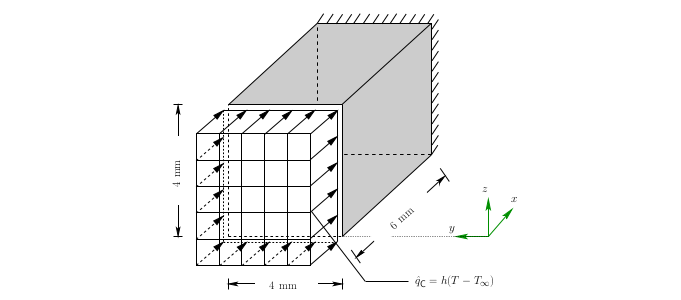
\includegraphics[width=.85\textwidth]{figures/setup_2nd_danilovskaya.png}
%   \caption{Setup for the second Danilovskaya problem. Initial geometry and prescirbed heat convection boundary condition \(\hat q_C\).}
%   \label{fig:setup_2nd_danilovskaya}
% \end{figure}
%
% The simulation performed in three spatial dimensions.
% However, all displacement degrees of freedom in the \(y\)- and \(z\)-directions are fixed, such that a quasi-one-dimensional motion is produced.
% The body is assumed to be mechanically constrained and thermally insulated.
%
% The mechanical and thermal field properties are given in Table~\ref{tab:snd_danilovskaya_description}, where \(\bar{h}\) denotes the kinematic heat transfer coefficient, defined as \(\bar{h}=\frac{h}{\rho C_V}\) with the linear heat transfer coefficient \(h\).
% Furthermore, the values for the thermal conductivity \(k\), the coefficient of thermal expansion \(\alpha_{T}\), the constant initial temperature \(T_{0}\), as well as an ambient temperature \(T_{\infty}\) are given.
% The elastic constants characterizing the material are the Young's modulus \(E\) and Poisson's rate \(v\).
% A linear thermoelastic material is chosen according to the model described in \cite{armero_new_1992}.
%
% In the literature (\cite{farhat_unconditionally_1991}, \cite{tosaka_boundary_1991}, \cite{tamma_effective_1992}, \cite{tanaka_application_1995}), the density \(\rho\) and the heat capacity \(C_V\) are not divulged, and can in theory, be chosen arbitrarily according a dimensionless termomechanical parameter \(\delta\).
% However, to achieve a direct comparison with the results in \cite{tanaka_application_1995}, \cite{danowski_computational_2014} chose after calibration \(\rho=\SI{7.850}{\kilo\gram\meter^{-3}}\), yielding \(C_V = \SI[exponent-mode=engineering]{0.821}{\joule\kg^{-1}\kelvin^{-1}}\).
% These values are adopted here as well.
%
% \begin{table}
%   \centering
%   \caption{Material properties, and initial and boundary conditions for the second Danilovskaya problem.}
%   \label{tab:snd_danilovskaya_description}
%   \begin{tabular}{ccS[exponent-mode=engineering]}
%   \multicolumn{2}{c}{Material Properties} & {\vphantom{\Big |}Effective value}\\
%   \hline\hline
%   \vphantom{\Big |}Density \(\rho\) & (\si{\newton\second^2\milli\meter^{-4}}) & 7850e-12\\
%   \vphantom{\Big |}Young's modulus \(E\) & (\si{\newton\milli\meter^{-2}}) & 210e3\\
%   \vphantom{\Big |}Poisson's coefficient \(\nu\) & - & 0.3\\
%   \vphantom{\Big |}Conductivity \(k\) & (\si{\newton\second^{-1}\kelvin^{-1}}) & 1.03\\
%   \vphantom{\Big |}Heat capacity \(C_V\) & (\si{\milli\meter^2\second^{-2}\kelvin^{-1}}) & 0.821e6\\
%   \vphantom{\Big |}\makecell[c]{Coefficient of\\ thermal expansion} \(\alpha_T\) & (\si{\kelvin^{-1}}) & 1.1e-6\\
%   \hline
%   \multicolumn{2}{c}{Boundary Conditions\vphantom{\Big |}} & \\\hline
%   \vphantom{\Big |}Dimension \(l_x\) & (\si{\milli\meter}) & 6\\
%   \vphantom{\Big |}Dimension \(l_y\) & (\si{\milli\meter}) & 4\\
%   \vphantom{\Big |}Dimension \(l_z\) & (\si{\milli\meter}) & 4\\
%   \makecell[c]{Kinetic heat\\ convection coefficient} \(\bar h\) & (\si{\milli\meter\second^{-1}}) & 100e-3\\
%   \multicolumn{3}{c}{\vphantom{\Big |}All mechanical degrees of freedom fixed in the \(y\)- and \(z\)-directions.}\\
%   \hline
%   \multicolumn{2}{c}{Initial Conditions\vphantom{\Big |}} & \\\hline
%   \vphantom{\Big |}Ambient temperature \(T_\text{env}\) & (\si{\kelvin}) & {373.15}\\
%   Intial temperature \(T_0\) & (\si{\kelvin}) & {273.15}\\
%   \hline
%   \multicolumn{2}{c}{Reference value \vphantom{\Big |}} & \\\hline
%   \vphantom{\Big |}Temperature at point \(E\) (\(x=\SI{1}{\milli\meter}\)) & (\si{\kelvin}) & \\
%   \hline\hline
%   \end{tabular}
% \end{table}
%
% The discretisation for both the mechanical and thermal field contains each \(n_{x} \times n_{y} \times n_{z}=12 \times\) \(4 \times 4\) Hex 8 elements.
% The simulation time is \(t=\SI{4}{\second}\), with a time-step size of \(\Delta t=\SI{0.001}{\second}\).
% Moreover, a one-step- \(\theta\) time integration is chosen with the value \(\theta=0.5\), resulting in a CrankNicolson scheme for the temperature field, and quasi-static approach for the mechanical field.
% Displacements and temperatures are evaluated at the centre point of the plane at \(x=\SI{1}{\milli\meter}\).

\section{Expansion of a thermoelastic thick-walled cylinder}

The following numerical example concerns the quasi-static finite strain thermo-elastic expansion of an infinitely long thick-walled cylinder, as presented in \cite{ibrahimbegovic_thermodynamics_2009}.
\cite{armero_new_1992} and \cite{erbts_accelerated_2012} also present results regarding this problem, although the dimensions of the cylinder considered there are different from the ones used in the present work.
The example is comprised by an infinitely long cylinder with an inner radius of \(r_{0}=\SI{5}{\milli\meter}\) and an outer radius of \(r_{1}=\SI{15}{\milli\meter}\).
A displacement driven problem is produced enforcing an increasing radial displacement at the inner radius with a constant rate of \(\dot{u}_{0}\).
Following \cite{ibrahimbegovic_thermodynamics_2009}, the maximum displacement is set to \SI{10}{\milli\meter}, which clearly involves large deformations.
Zero heat flux is imposed at the inner radius, whereas the temperature at the outer radius is set to a reference temperature \(T_{0}\).
The initial temperature of the cylinder is also \(T_0\).
A sketch of the problem, incuding the initial and boundary conditions described, is shown in Figure~\ref{fig:problem_description}.
A decoupled Neo-Hookean free energy function characterizes the thermo-elastic material considered in this analysis, in accordance with \cite{armero_new_1992}.
All material and model properties can be found in Table~\ref{tab:expansion_thick_walled_cylinder}.

\begin{figure}[htbp]
  \centering
  \def\svgwidth{1.0\linewidth}
  \footnotesize
  \input{figures/thick_cylinder_problem_description.pdf_tex}
  \caption{Initial and boundary conditions considered in the quasi-static finite strain thermo-elastic expansion of an infinitely long thick-walled cylinder, and corresponding FEM mesh (QUAD4) used.}
\label{fig:problem_description}
\end{figure}

\begin{table}
  \centering
  \caption{Material properties, and initial and boundary conditions for the problem concerning the quasi-static finite strain thermo-elastic expansion of an infinitely long thick-walled cylinder.}
\label{tab:expansion_thick_walled_cylinder}
  \begin{tabular}{lccS[exponent-mode=engineering]}
  \multicolumn{3}{c}{Material Properties} & {\vphantom{\Big |}Effective value}\\
  \hline\hline
  \vphantom{\Big |}Density & \(\rho\) & (\si{\newton\second^2\milli\meter^{-4}}) & 7.8e-9\\
  \vphantom{\Big |}Bulk modulus & \(\kappa\) & (\si{\newton\milli\meter^{-2}}) & 164206\\
  \vphantom{\Big |}Shear modulus & \(\mu\) & (\si{\newton\milli\meter^{-2}}) & 80140\\
  \vphantom{\Big |}Conductivity & \(k\) & (\si{\newton\second^{-1}\kelvin^{-1}}) & 45\\
  \vphantom{\Big |}Heat capacity & \(C_V\) & (\si{\milli\meter^2\second^{-2}\kelvin^{-1}}) & 460e6\\
  \vphantom{\Big |}Coefficient of thermal expansion & \(\alpha_T\) & (\si{\kelvin^{-1}}) & {\SI[exponent-mode=engineering]{0}{} - \SI[exponent-mode=engineering]{1.5e-4}{}}\\
  \hline
  \multicolumn{3}{c}{Boundary Conditions\vphantom{\Big |}} & \\\hline
  \vphantom{\Big |}Inner radius & \(r_0\) & (\si{\milli\meter}) & 5\\
  \vphantom{\Big |}Outer radius & \(r_1\) & (\si{\milli\meter}) & 15\\
  \vphantom{\Big |}Inner radius rate of displacement & \(\dot u_0\) & (\si{\milli\meter\second^{-1}}) & {0.1; 0.25; 0.5}\\
  \vphantom{\Big |}Heat at inner radius & \(q_1\) & (\si{\newton\second^{-1}\milli\meter^{-1}}) & 0\\
  \vphantom{\Big |}Temperature outer radius & \(T_1\) & (\si{\kelvin}) & 273.15\\
  % \multicolumn{3}{c}{\vphantom{\Big |}All mechanical degrees of freedom fixed in the \(y\)- and \(z\)-directions.}\\
  \hline
  \multicolumn{3}{c}{Initial Conditions\vphantom{\Big |}} & \\\hline
  Intial temperature & \(T_0\) & (\si{\kelvin}) & {273.15}\\
  \hline
  \multicolumn{3}{c}{Reference value \vphantom{\Big |}} & \\\hline
  \vphantom{\Big |}Temperature at inner radius (\(r=r_0\)) & (\si{\kelvin}) & \\
  \hline\hline
  \end{tabular}
\end{table}

A plain strain analysis is used to solve the problem, implying a null displacement and heat flux in the axial direction.
Linear quadratic elements (QUAD4) are used in the FEM discretization employed.
Thanks to the axial symmetry of the problem, only one-fourth of the cylinder is considered, as depicted in Figure~\ref{fig:problem_description}.
Except when explicitly indicated, the mesh employed contains 2601 nodes and 2500 elements.

The displacement is imposed in 200 equal time steps $\Delta t = \SI{0.1}{\second}$,
A quasi-static solution is computed for the mechanical problem using a backward Euler integration scheme and the transient temperature field is integrated in time employing the generalised-$\alpha$ method with $\rho_{\infty,T}=1.0$.

\subsection{Validation of the Numerical Results}

To validate the results presented in this work regarding the quasi-static finite strain thermo-elastic expansion of an infinitely long thick-walled cylinder, the problem is solved considering an \(\alpha_T = \SI{1.65e-4}{\kelvin^{-1}}\) and a \(\alpha_T = \SI{1.65e-5}{\kelvin^{-1}}\), at three different displacement rates for the inner radius, (\(\dot u_0 = \SIlist{0.1; 0.25; 0.5}{\milli\meter\second^{-1}}\)).
Reference results for this configuration of the problem are available in \cite{ibrahimbegovic_thermodynamics_2009}, and provide a suitable comparison for the validation of the results obtained in the present work.
There is however one caveat, since in \cite{ibrahimbegovic_thermodynamics_2009} the results reported are supposedly for coefficients of thermal expansion equal to \SI{e-5}{\kelvin^{-1}} and \SI{e-4}{\kelvin^{-1}}.
The values used in the present work are the ones leading to the best fit between the present and the reference results.
The values chosen for the expansion coefficient lead to, so-called, weak and strong coupling.
The use of the latter value for the thermal expansion coefficient leads to instabilities when using a fixed-point explicit or implicit scheme with the isothermic split \citep{ibrahimbegovic_thermodynamics_2009, erbts_accelerated_2012}.

The temperature evolutions as a function of inner raidus displacement for a point located at the inner radius of the cylinder are presented in Figures~\ref{fig:thick_cylinder_validation_inner_radius_temperature_weak_coupled_quad4fbar} and \ref{fig:thick_cylinder_validation_inner_radius_temperature_strong_coupled_quad4fbar} chosing \(\alpha_T = \SI{1.65e-5}{\kelvin^{-1}}\) and \(\alpha_T =\SI{1.65e-4}{\kelvin^{-1}}\), respectively.
Figure~\ref{fig:thick_cylinder_temp_dist} presents the temperature distribution in half a transversal section of the thick-walled cylinder at increasing inner radius displacements.
A good agreement between the numerical results obtained in the present work and the ones found in \cite{ibrahimbegovic_thermodynamics_2009} can be observed for all displacement rates considered.
The temperature at the inner radius suffers a sharp decrease and then, as the displacement increases, tends to the reference temperature \(T_0\).
This decrease is due to the thermo-elastic heating effect and the fact that heat cannot be supplied from the outer radius fast enough to prevent this drop in temperature near the inner radius.

\begin{figure}[htbp]
  \centering
  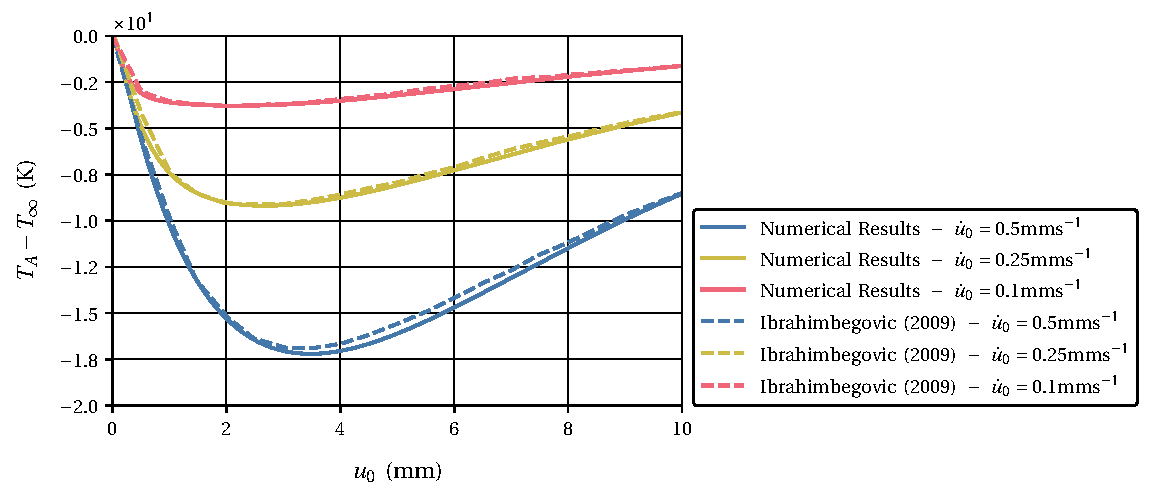
\includegraphics[width=.85\textwidth]{thick_cylinder_validation_inner_radius_temperature_weak_coupled_quad4fbar}
  \caption{Difference between the temperature at the inner radius and the reference temperature for the expansion of the thick-walled cylinder with \(\alpha_T=\SI{1.65e-5}{\kelvin^{-1}}\) and at different displacement rates for the inner radius (\(\dot u_0 = \SIlist{0.1; 0.25; 0.5}{\milli\meter\second^{-1}}\)}
\label{fig:thick_cylinder_validation_inner_radius_temperature_weak_coupled_quad4fbar}

\end{figure}
\begin{figure}[htbp]
  \centering
  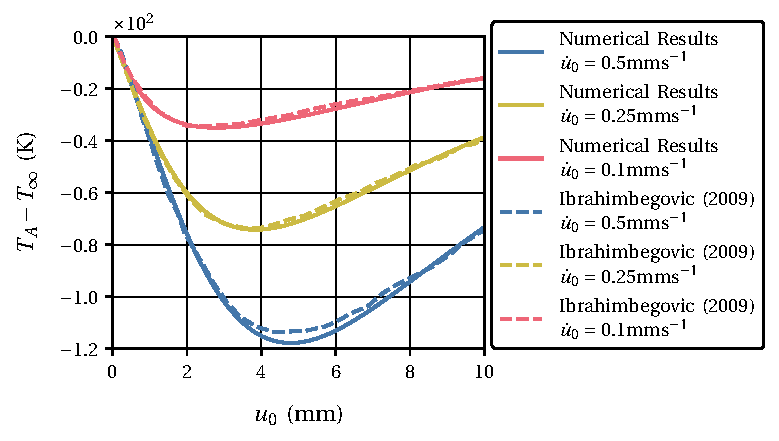
\includegraphics[width=.85\textwidth]{thick_cylinder_validation_inner_radius_temperature_strong_coupled_quad4fbar}
  \caption{Difference between the temperature at the inner radius and the reference temperature for the expansion of the thick-walled cylinder with \(\alpha_T=\SI{1.65e-4}{\kelvin^{-1}}\) and at different displacement rates for the inner radius (\(\dot u_0 = \SIlist{0.1; 0.25; 0.5}{\milli\meter\second^{-1}}\)}
\label{fig:thick_cylinder_validation_inner_radius_temperature_strong_coupled_quad4fbar}
\end{figure}

\begin{figure}[htbp]
  \centering
  \def\svgwidth{1.0\linewidth}
  \footnotesize
  \input{figures/thick_cylinder_temp_dist.pdf_tex}
  \caption{Temperature distribution in half a transversal section of the thick-walled cylinder at increasing inner radius displacements for \(\alpha_T=\SI{1.65e-4}{\kelvin^{-1}}\) and \(\dot u_0 = \SI{0.5}{\milli\meter\second^{-1}}\).}
\label{fig:thick_cylinder_temp_dist}
\end{figure}

\FloatBarrier

\subsection{Evaluation and comparison of implicit solution methods for the coupled problem}

The following contains the results concerning the evaluation and comparison of the implicit solution methods for coupled problems considered in this work.
The discussion starts with the methods that require only one evalution of the residual per nonlinear iteration.
The Broyden-like family of methods fall into this category too but are considered by themselves and are presented next.
The Newton-Krylov methods are also analysed, followed by the vector extrapolation methods in cycling mode.
The discussion ends with the comparison bewteen the best methods in each class and effect of predictors on the efficiency of the implicit methods.

The analysis presented is based mainly on three pieces of information.
The first concerns how the residual evolves as a function of the nonlinear iterations.
The second is the number of function evaluations needed to solve the coupled problem to the desired accuracy at each time step.
The third is the total number of residual evaluations needed to solve the coupled problem to the desired accuracy as a function of the thermal expansion coefficient.
The larger the thermal expansion coefficient the stronger the coupling between the thermal and mechanical fields, and the harder the problem is to solve.
The evaluation of the residual implies the solution of the thermal and mechanical problems one after the other, and takes the lion's share of computational time.
Regarding conclusions related to efficiency, it suffices when comparing methods of the same class to consider the number of residual evaluations.
The computational time will only be analyzed in the comparison bewteen the best methods of each class.

Only the displacement rate \(\dot u_0 = \SI{0.5}{\milli\meter\second^{-1}}\) is considered, with the thermal expansion coefficient varying from \SI{0}{\kelvin^{-1}} to \SI{1.5e-4}{\kelvin^{-1}}.

\subsubsection{Methods with only one residual evaluation per iteration}

The methods with only one residual evaluation per nonlinear iteration considered are the fixed-point method (see Section~\ref{sec:fixed_point_approach}), the underrelaxation method (see Section~\ref{sec:underrelaxation}), the Aitken relaxation (see Section~\ref{sec:aitken_relaxation}) and Broyden's method, Type I and II (see Section~\ref{sec:multisecant}).
These are, a priori, the most parcimonious methods regarding residual evaluations, as only one is performed per nonlinear iteration.
The underrelaxation is performed with \(\omega = 0.5\), and the first relaxation coefficient for the Aitken relaxation is also set to 0.5.

Figure~\ref{fig:thick_cylinder_single_iter_residual_1st_time_step_quad4fbar_pred} presents the residual in percentage as a function of the number of nonlinear iterations in the first time step with \(\alpha_T=\SI{1.5e-4}{\kelvin^{-1}}\) and \(\dot u_0 =\SI{0.5}{\milli\meter\second^{-1}}\).
As reported by \cite{erbts_accelerated_2012}, the fixed-point scheme is unable to converge for this value of the thermal expansion coefficient.
The other methods all converge approximately linearly, with the Broyden methods and the Aitken relaxation method taking the same number of nonlinear iterations/residual evaluations.
Furthermore, the two Broyden methods are almost visually undistinguishable.
The underrelaxation methods takes more iterations to converge.
This could, however, possibly be improved by tuning the relaxation coefficient further.

\begin{figure}[htbp]
  \centering
  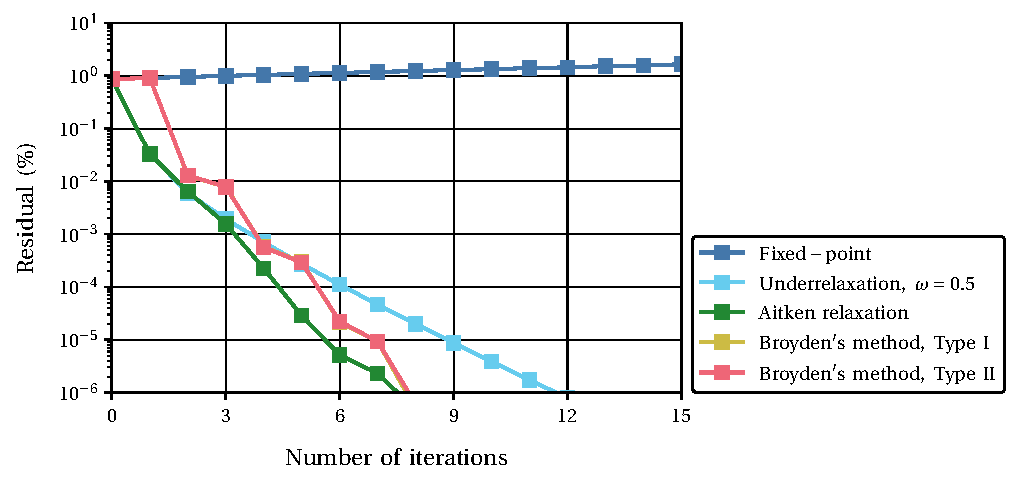
\includegraphics[width=.85\textwidth]{thick_cylinder_single_iter_residual_1st_time_step_quad4fbar_pred}
  \caption{Residual in percentage as a function of the number of nonlinear iterations in the first time step for the implicit methods that perform only one evaluation per nonlinear iteration in the solution of the quasi-static expansion of a thermoelastic thick-walled cylinder with \(\alpha_T=\SI{1.5e-4}{\kelvin^{-1}}\) and \(\dot u_0 =\SI{0.5}{\milli\meter\second^{-1}}\). }
\label{fig:thick_cylinder_single_iter_residual_1st_time_step_quad4fbar_pred}
\end{figure}

Figure~\ref{fig:thick_cylinder_single_iter_n_iter_time_quad4fbar_pred} presents the number of nonlinear iterations/residual evaluations needed to solve the coupled thermomechanical problem at each time step and the total (cumulative) number of iterations needed.
The strength of the coupling, tightly connected to the difficulty in solving the coupled problem and hence the number of nonlinear iterations needed to solve it, seems to be approximately uniform across the displacement range considered, with a slight decrease as the displacement increases.
The Broyden methods show a very similar behavior, besting the Aitken relaxation at each time step by at most one or two nonlinear iterations.
This leads, however, to a sizable difference in the total number of function evaluations needed to solve the problem from start to finish.
The underrelaxation method under performs again, showing even more difficulty in solving the problem as the displacement increases.

\begin{figure}[htbp]
  \centering
  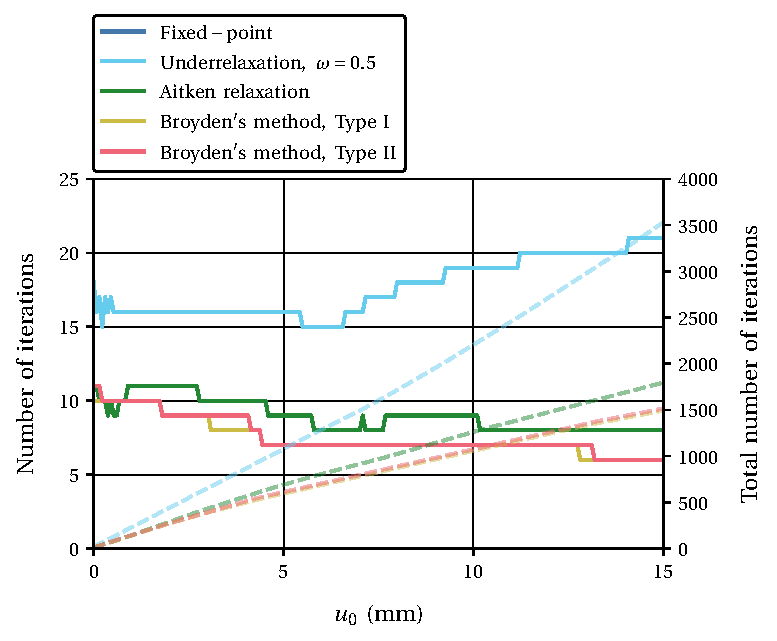
\includegraphics[width=.85\textwidth]{thick_cylinder_single_iter_n_iter_time_quad4fbar_pred}
  \caption{Number of nonlinear iterations needed to solve the coupled problem at each time step and the total number of iterations needed to solve the coupled problem for the implicit methods that perform only one evaluation per nonlinear iteration  in the solution of the quasi-static expansion of a thermoelastic thick-walled cylinder with \(\alpha_T=\SI{1.5e-4}{\kelvin^{-1}}\) and \(\dot u_0 =\SI{0.5}{\milli\meter\second^{-1}}\).}
\label{fig:thick_cylinder_single_iter_n_iter_time_quad4fbar_pred}
\end{figure}

Figure~\ref{fig:thick_cylinder_single_iter_n_iter_coupl_strength_quad4fbar_pred} presents the total number of residual evaluations, in this case corresponding also to the total number of nonlinear iterations, as a function of the thermal expansion coefficient, which controls the strength of the coupling between the thermal and the mechanical fields, respectively.
The number of residual evaluations coorelates strongly with the total CPU time, accounting for the largest portion of the computational time.
The most efficient methods are the two Broyden methods, followed by the Aitken relaxation.
The underrelaxation method performs poorly through out the range of values considered for the thermal expansion coefficient and the fixed-point becomes incresingly slow as the coupling gets stronger eventually failing to converge for \(\alpha_T=\SI{1.5e-4}{\kelvin^{-1}}\).

\begin{figure}[htbp]
  \centering
  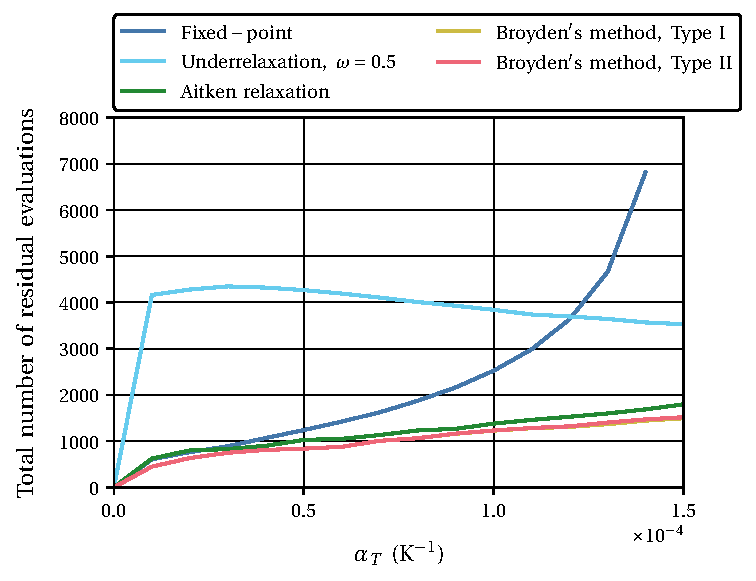
\includegraphics[width=.85\textwidth]{thick_cylinder_single_iter_n_iter_coupl_strength_quad4fbar_pred}
  \caption{Total number of residual evaluations as a function of the thermal expansion coefficient for the implicit methods that perform only one evaluation per nonlinear iteration in the solution of the quasi-static expansion of a thermoelastic thick-walled cylinder with \(\alpha_T=\SIrange{0}{1.5e-4}{\kelvin^{-1}}\) and \(\dot u_0 =\SI{0.5}{\milli\meter\second^{-1}}\).}
\label{fig:thick_cylinder_single_iter_n_iter_coupl_strength_quad4fbar_pred}
\end{figure}

\FloatBarrier

\subsubsection{Broyden-like method}

The Broyden-like methods considered (see Section~\ref{sec:multisecant}) employ as group sizes \(s=1,\ 2,\ 3,\ 6\) with a maximum number of previous iterations available equal to 6.
The mixing parameters considered are \(\beta=-1,\ \num{2e-3},\ \num{2e-2}\).
Their choice is based on prior tuning, which, however, was not exhaustive.
All combinations are also considered with both Type I and Type II updating for the approximation to the Jacobian.

Figures~\ref{fig:thick_cylinder_broyden_like_type_i_residual_1st_time_step_quad4fbar_pred} and \ref{fig:thick_cylinder_broyden_like_type_ii_residual_1st_time_step_quad4fbar_pred} present the residual in percentage as a function of the number of nonlinear iterations in the first time step with \(\alpha_T=\SI{1.5e-4}{\kelvin^{-1}}\) and \(\dot u_0 =\SI{0.5}{\milli\meter\second^{-1}}\) for Broyden-like methods with Type I and Type II updates, respectively.
There is no marked difference bewteen methods that employ a Type I and Type II update.
However, the choice for the mixing parameter and the group size leads to different behaviors for the residual.
For \(\beta=-1\), the methods using \(s=1\), 2 and 3 behave much the same with an approximately linear convergence rate, and are the ones needing the fewest iterations to reach the desired accuracy.
For \(s=6\) the residual behaves differently, plateuaing for several nonlinear iterations.
Despite this, it only takes a few more iterations to converge when compared with the methods employing \(s=1\), 2 and 3.
When \(\beta=\num{2e-3}\) and \num{2e-2} are utilized, they exihibt a similar trend, with residual plateuas for a few iterations before decreasing.
This behavior can partly be explained by the fact that the implementation used follows the suggestion found in \cite{fang_two_2009}, where due to memory concerns, the approximation to the inverse of the Jacobian is only updated after the next group of residual evaluations has been completly filled (see Section~\ref{sec:multisecant}).
This can lead to a momentaneous poor approximation to the inverse of the Jacobain and thus stagnation of the residual.
The choice of \(\beta=\num{2e-2}\) seems to lead to slightly fewer iterations before the desired accuracy is reached.

\begin{figure}[htbp]
  \centering
  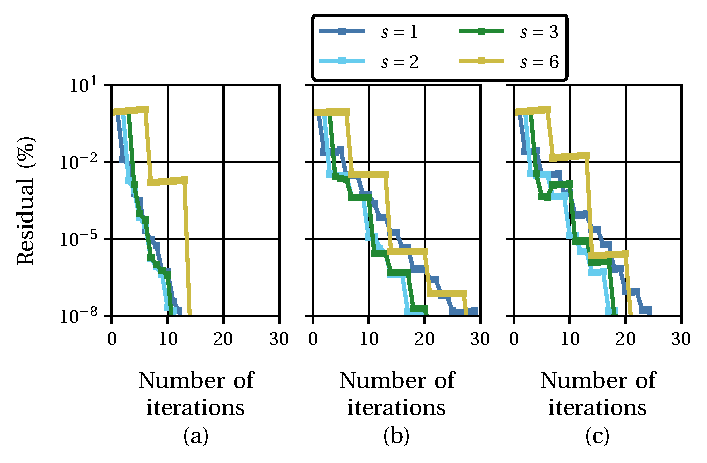
\includegraphics[width=.85\textwidth]{thick_cylinder_broyden_like_type_i_residual_1st_time_step_quad4fbar_pred}
  \caption{Residual in percentage as a function of the number of nonlinear iterations in the first time step for Broyden-like methods with Type I update and group sizes \(s=1\), 2, 4 and 6: (a) \(\beta=-1\), (b) \(\beta=\num{2e-3}\), and (c) \(\beta=\num{2e-2}\) in the solution of the quasi-static expansion of a thermoelastic thick-walled cylinder with \(\alpha_T=\SI{1.5e-4}{\kelvin^{-1}}\) and \(\dot u_0 =\SI{0.5}{\milli\meter\second^{-1}}\).}
\label{fig:thick_cylinder_broyden_like_type_i_residual_1st_time_step_quad4fbar_pred}
\end{figure}

\begin{figure}[htbp]
  \centering
  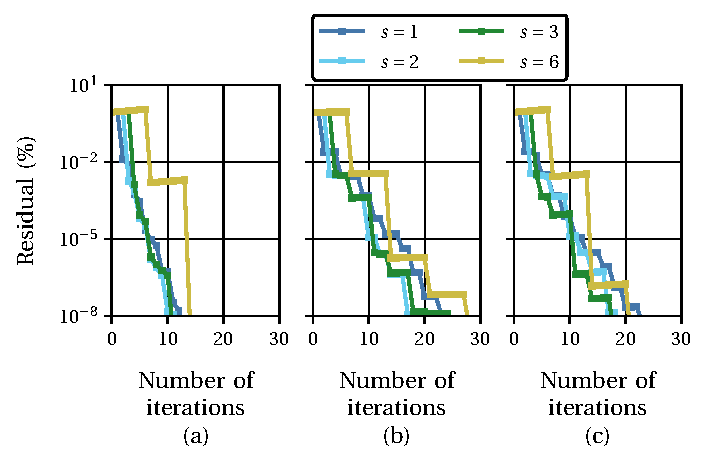
\includegraphics[width=.85\textwidth]{thick_cylinder_broyden_like_type_ii_residual_1st_time_step_quad4fbar_pred}
  \caption{Residual in percentage as a function of the number of nonlinear iterations in the first time step for Broyden-like methods with Type II update and group sizes \(s=1\), 2, 4 and 6: (a) \(\beta=-1\), (b) \(\beta=\num{2e-3}\), and (c) \(\beta=\num{2e-2}\) in the solution of the quasi-static expansion of a thermoelastic thick-walled cylinder with \(\alpha_T=\SI{1.5e-4}{\kelvin^{-1}}\) and \(\dot u_0 =\SI{0.5}{\milli\meter\second^{-1}}\).}
\label{fig:thick_cylinder_broyden_like_type_ii_residual_1st_time_step_quad4fbar_pred}
\end{figure}

Figures~\ref{fig:thick_cylinder_broyden_like_type_i_n_iter_time_quad4fbar_pred} and \ref{fig:thick_cylinder_broyden_like_type_ii_n_iter_time_quad4fbar_pred} present the number of nonlinear iterations/number of function evaluations needed to solve the coupled problem at each time step and the total (cumulative) number of iterations needed.
Again the differences bewteen the Broyden-like methods using Type I and Type II updates is not pronounced.
Perhaps the most noticeable difference is for \(\beta=\num{2e-3}\) and \num{2e-2}, where the total number of iterations needed to solve the coupled thermomechanical problem for the Type I methods oscillates more strongly between time steps.
For \(\beta=-1\), the methods using group sizes of 1, 2 and 3 display a higher efficiency, which disappears as the displacement increases.
For \(\beta=\num{2e-2}\) and \num{2e-3}, the results seem to indicate the need for fewer iterations when using group sizes of 2 and 3.

\begin{figure}[htbp]
  \centering
  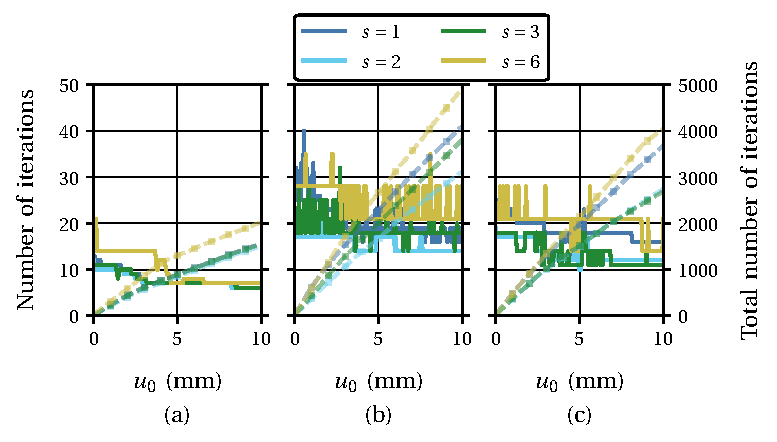
\includegraphics[width=.85\textwidth]{thick_cylinder_broyden_like_type_i_n_iter_time_quad4fbar_pred}
  \caption{Number of nonlinear iterations needed to solve the coupled problem at each time step and the total number of iterations needed to solve the coupled problem for Broyden-like methods with Type I update and group sizes \(s=1\), 2, 4 and 6: (a) \(\beta=-1\), (b) \(\beta=\num{2e-3}\), and (c) \(\beta=\num{2e-2}\) in the solution of the quasi-static expansion of a thermoelastic thick-walled cylinder with \(\alpha_T=\SI{1.5e-4}{\kelvin^{-1}}\) and \(\dot u_0 =\SI{0.5}{\milli\meter\second^{-1}}\).}
\label{fig:thick_cylinder_broyden_like_type_i_n_iter_time_quad4fbar_pred}
\end{figure}

\begin{figure}[htbp]
  \centering
  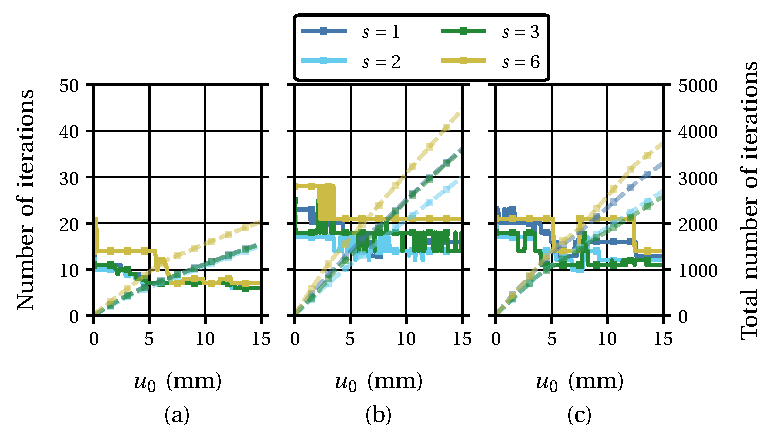
\includegraphics[width=.85\textwidth]{thick_cylinder_broyden_like_type_ii_n_iter_time_quad4fbar_pred}
  \caption{Number of nonlinear iterations needed to solve the coupled problem at each time step and the total number of iterations needed to solve the coupled problem for Broyden-like methods with Type II update and group sizes \(s=1\), 2, 4 and 6: (a) \(\beta=-1\), (b) \(\beta=\num{2e-3}\), and (c) \(\beta=\num{2e-2}\) in the solution of the quasi-static expansion of a thermoelastic thick-walled cylinder with \(\alpha_T=\SI{1.5e-4}{\kelvin^{-1}}\) and \(\dot u_0 =\SI{0.5}{\milli\meter\second^{-1}}\).}
\label{fig:thick_cylinder_broyden_like_type_ii_n_iter_time_quad4fbar_pred}
\end{figure}

Figures~\ref{fig:thick_cylinder_broyden_like_type_i_n_iter_coupl_strength_quad4fbar_pred} presents the total number of residual evaluations as a function of the thermal expansion coefficient, respectively, for the Broyden-like methods with Type I update considered.
The same results are presented in Figures~\ref{fig:thick_cylinder_broyden_like_type_ii_n_iter_coupl_strength_quad4fbar_pred} for the Broyden-like methos with Type II update.
The most efficient methods employ a mixing parameter equal to \(\beta=-1\) and group sizes equal to 1, 2 and 3.
The choices of \num{2e-3} and \num{2e-2} for the mixing parameter lead to less efficient methods, which need a larger amount of residual evaluations and thus require more CPU time to solve the coupled thermomechanical problem completly.

\begin{figure}[htbp]
  \centering
  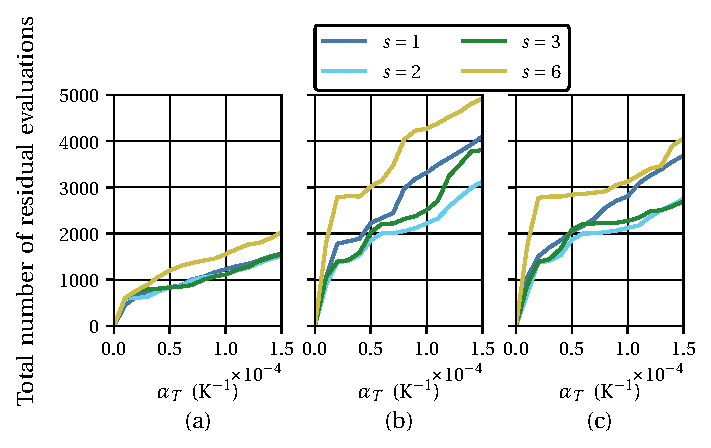
\includegraphics[width=.85\textwidth]{thick_cylinder_broyden_like_type_i_n_iter_coupl_strength_quad4fbar_pred}
  \caption{Total number of residual evaluations as a function of the thermal expansion coefficient for the implicit methods for Broyden-like methods with Type I update and group sizes \(s=1\), 2, 4 and 6: (a) \(\beta=-1\), (b) \(\beta=\num{2e-3}\), and (c) \(\beta=\num{2e-2}\) in the solution of the quasi-static expansion of a thermoelastic thick-walled cylinder with \(\alpha_T=\SIrange{0}{1.5e-4}{\kelvin^{-1}}\) and \(\dot u_0 =\SI{0.5}{\milli\meter\second^{-1}}\).}
\label{fig:thick_cylinder_broyden_like_type_i_n_iter_coupl_strength_quad4fbar_pred}
\end{figure}

\begin{figure}[htbp]
  \centering
  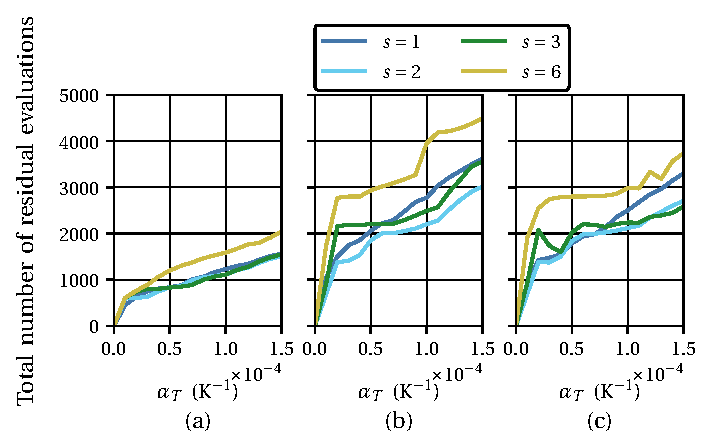
\includegraphics[width=.85\textwidth]{thick_cylinder_broyden_like_type_ii_n_iter_coupl_strength_quad4fbar_pred}
  \caption{Total number of residual evaluations as a function of the thermal expansion coefficient for Broyden-like methods with Type II update and group sizes \(s=1\), 2, 4 and 6: (a) \(\beta=-1\), (b) \(\beta=\num{2e-3}\), and (c) \(\beta=\num{2e-2}\) in the solution of the quasi-static expansion of a thermoelastic thick-walled cylinder with \(\alpha_T=\SIrange{0}{1.5e-4}{\kelvin^{-1}}\) and \(\dot u_0 =\SI{0.5}{\milli\meter\second^{-1}}\).}
\label{fig:thick_cylinder_broyden_like_type_ii_n_iter_coupl_strength_quad4fbar_pred}
\end{figure}

\FloatBarrier

\subsubsection{Newton-GMRES method}

The Newton-Krylov method examined here uses as the Krylov subspace solver the GMRES method (see Section~\ref{sec:newton_krylov}).
Different forcing terms are employed.
The values considered are \(\eta=\num[print-unity-mantissa=false]{e-1}\), \num[print-unity-mantissa=false]{e-3} and \num[print-unity-mantissa=false]{e-5}.
The Eisenstat-Walker scheme for the adpative choice of the forcing term is also utilized.

Figure~\ref{fig:thick_cylinder_newton_krylov_residual_1st_time_step_quad4fbar_pred} presents the residual in percentage as a function of the number of nonlinear iterations in the first time step with \(\alpha_T=\SI{1.5e-4}{\kelvin^{-1}}\) and \(\dot u_0 =\SI{0.5}{\milli\meter\second^{-1}}\).
For \(\eta=\num{e-5}\), the Newton-GMRES method converges quadractly since the Newton system is solved to a finer accuracy, and thus closely approximates the Newton-Raphson scheme.
As \(\eta\) increases the convergence rate as a function of the number of nonlinear iterations slows down.
The method employing the Eisenstat-Walker scheme performs similarly to the method using a constant forcing term equal to \num{e-1}.
Keep in mind, that within each nonlinear iteration the Newton-Krylov methods may evaluate the function several times, such that converging in a fewer number of nonlinear iterations does not necesseraly imply a more efficient method regarding computational time spent solving the coupled thermomechanical problem.

\begin{figure}
  \centering
  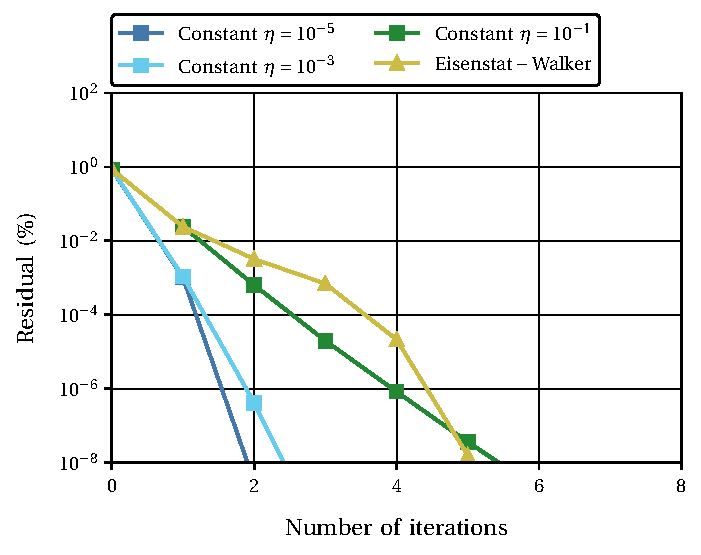
\includegraphics[width=.85\textwidth]{thick_cylinder_newton_krylov_residual_1st_time_step_quad4fbar_pred}
  \caption{Residual in percentage as a function of the number of nonlinear iterations in the first time step for the Newton-GMRES method with a constant forcing term (\(\eta=\num{1e-5},\ \num{1e-3},\ \num{1e-1}\)) and the Eisenstat-Walker scheme in the solution of the quasi-static expansion of a thermoelastic thick-walled cylinder with \(\alpha_T=\SI{1.5e-4}{\kelvin^{-1}}\) and \(\dot u_0 =\SI{0.5}{\milli\meter\second^{-1}}\).}
\label{fig:thick_cylinder_newton_krylov_residual_1st_time_step_quad4fbar_pred}
\end{figure}

Figure~\ref{fig:thick_cylinder_newton_krylov_n_iter_time_quad4fbar_pred} presents the number of nonlinear iterations needed to solve the coupled problem at each time step and the total (cumulative) number of iterations needed.
The strength of the coupling seems to be approximately uniform across the displacement range considered, as the number of iteratins taken by each method remains approximately constant as the displacement increases.
As hinted by the results already discussed regarding the residual as a function of the nonlinear iterations in the first time step, the smaller the forcing the fewer the number of nonlinear iterations needed to solve the coupled problem at each time step.
The method that uses the Eisenstat-Walker scheme performs in a similar way to the method using a constant forcing term equal to \num{1e-1}.

\begin{figure}
  \centering
  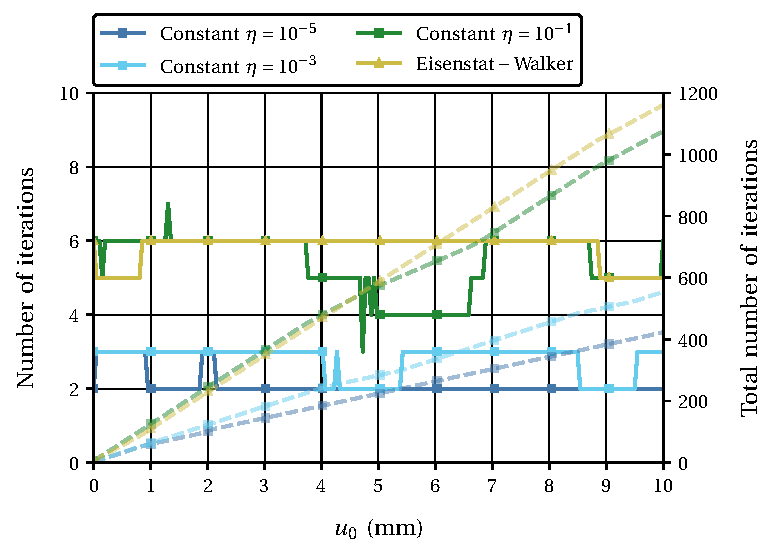
\includegraphics[width=.85\textwidth]{thick_cylinder_newton_krylov_n_iter_time_quad4fbar_pred}
  \caption{Number of nonlinear iterations needed to solve the coupled problem at each time step and the total number of iterations needed to solve the coupled problem for the Newton-GMRES method with a constant forcing term (\(\eta=\num{1e-5},\ \num{1e-3},\ \num{1e-1}\)) and the Eisenstat-Walker scheme in the solution of the quasi-static expansion of a thermoelastic thick-walled cylinder with \(\alpha_T=\SI{1.5e-4}{\kelvin^{-1}}\) and \(\dot u_0 =\SI{0.5}{\milli\meter\second^{-1}}\).}
\label{fig:thick_cylinder_newton_krylov_n_iter_time_quad4fbar_pred}
\end{figure}

Figures~\ref{fig:thick_cylinder_newton_krylov_n_iter_time_quad4fbar_pred} presents the total number of residual evaluations a function of the thermal expansion coefficient.
The most efficient Newton-GMRES methods analysed are the ones using a constant forcing term equal to \num{1e-5} and \num{1e-3}, followed by the method employing a constant forcing term equal to \num{1e-1} and then by the method utilizing the Eisenstat-Walker scheme.

\begin{figure}
  \centering
  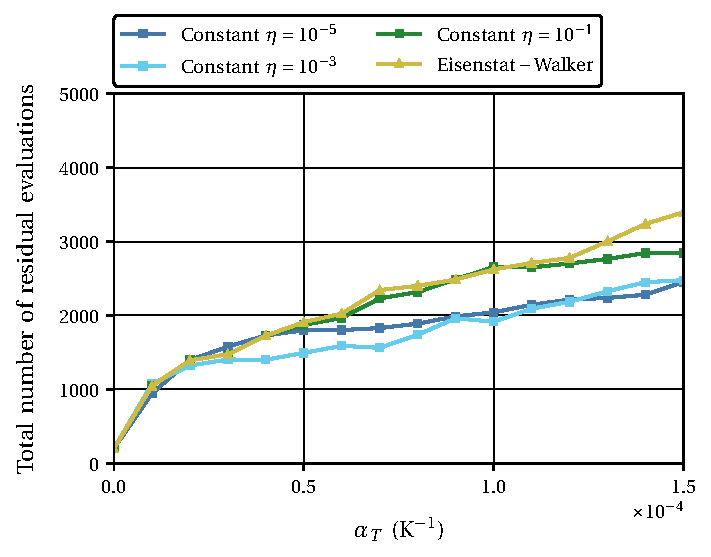
\includegraphics[width=.85\textwidth]{thick_cylinder_newton_krylov_n_iter_coupl_strength_quad4fbar_pred}
  \caption{Total number of residual evaluations as a function of the thermal expansion coefficient for the Newton-GMRES method with a constant forcing term (\(\eta=\num{1e-5},\ \num{1e-3},\ \num{1e-1}\)) and the Eisenstat-Walker scheme in the solution of the quasi-static expansion of a thermoelastic thick-walled cylinder with \(\alpha_T=\SIrange{0}{1.5e-4}{\kelvin^{-1}}\) and \(\dot u_0 =\SI{0.5}{\milli\meter\second^{-1}}\).}
\label{fig:thick_cylinder_newton_krylov_n_iter_coupl_strength_quad4fbar_pred}
\end{figure}

\FloatBarrier

\subsubsection{Polynomial vector extrapolation in cycling mode}

The polynomial vector extrapolation methods in cycling mode considered are the MPE and RRE, restriced to at most five evaluations of the residual function per nonlinear iteration.
Thus, the combinations analyzed are characterized by the ordered pairs \((n,k)=(1,1)\), \((1,2)\), \((1,3)\), \((2,1)\), \((2,2)\) and \((3,1)\) (see Section~\ref{sec:vector_extrapolation}).

Figure~\ref{fig:thick_cylinder_extrap_pol_residual_1st_time_step_quad4fbar_pred} presents the residual in percentage as a function of the number of nonlinear iterations in the first time step with \(\alpha_T=\SI{1.5e-4}{\kelvin^{-1}}\) and \(\dot u_0 =\SI{0.5}{\milli\meter\second^{-1}}\).
In general, the larger the number of residual evaluation per nonlinear iterations the faster rate of convergence.
Also, it seems that for the same number of residual evaluations per nonlinear iterations, e.g., \((n,k)=(1,3)\), \((2,2)\) and \((3,1)\) or \((n,k)=(1,2)\), \((2,1)\), it is more profitable to increase \(k\) than \(n\).
The results for the MPE and the RRE are very similar.

\begin{figure}[htbp]
  \centering
  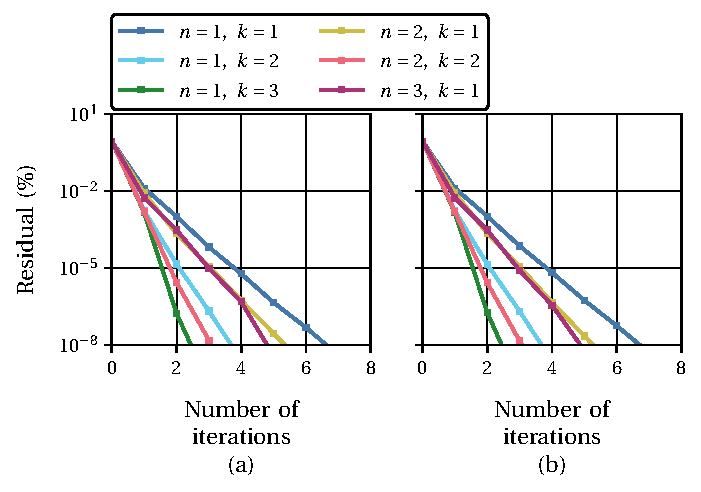
\includegraphics[width=0.9\textwidth]{thick_cylinder_extrap_pol_residual_1st_time_step_quad4fbar_pred}
  \caption{Residual in percentage as a function of the number of nonlinear iterations in the first time step for the polynomial vector extrapolation methods in cycling mode, MPE and RRE, restriced to at most five evaluations of the residual function per nonlinear iteration in the solution of the quasi-static expansion of a thermoelastic thick-walled cylinder with \(\alpha_T=\SI{1.5e-4}{\kelvin^{-1}}\) and \(\dot u_0 =\SI{0.5}{\milli\meter\second^{-1}}\).}
\label{fig:thick_cylinder_extrap_pol_residual_1st_time_step_quad4fbar_pred}
\end{figure}

Figure~\ref{fig:thick_cylinder_extrap_pol_n_iter_time_quad4fbar_pred} presents the number of residual evaluations needed to solve the coupled problem at each time step and the total (cumulative) number of iterations needed.
The number of nonlinear iterations needed to solve the coupled problem to the desired accuracy at each time step remains approximately constant with a slight decrease as the displacement increases.
As before, the MPE and RRE methods display very similar performances.
As hinted by the previous results regarding the residual, the methods with more residual evaluation per nonlinear iteration take in general less iterations to converge.

\begin{figure}[htbp]
  \centering
  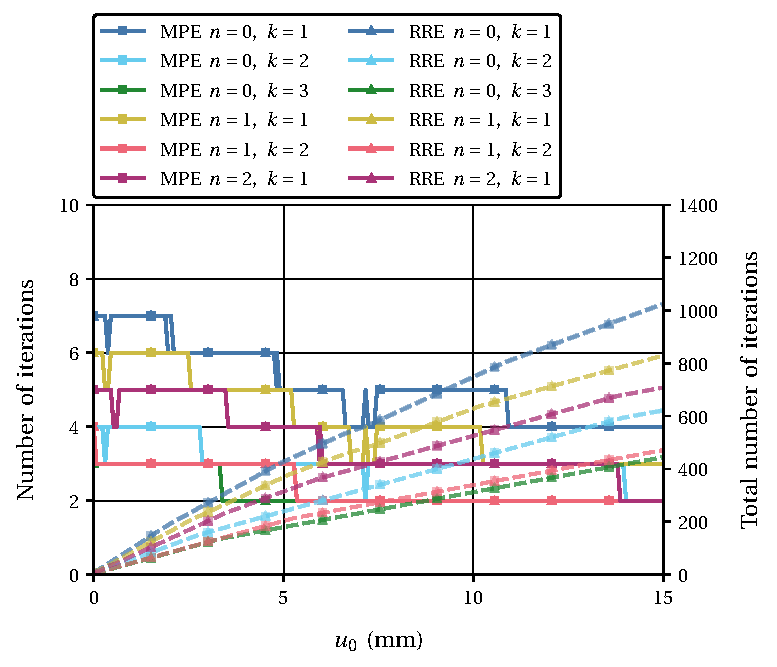
\includegraphics[width=0.9\textwidth]{thick_cylinder_extrap_pol_n_iter_time_quad4fbar_pred}
  \caption{Number of nonlinear iterations needed to solve the coupled problem at each time step and the total number of iterations needed to solve the coupled problem for the polynomial vector extrapolation methods in cycling mode, MPE and RRE, restriced to at most five evaluations of the residual function per nonlinear iteration in the solution of the quasi-static expansion of a thermoelastic thick-walled cylinder with \(\alpha_T=\SI{1.5e-4}{\kelvin^{-1}}\) and \(\dot u_0 =\SI{0.5}{\milli\meter\second^{-1}}\).}
\label{fig:thick_cylinder_extrap_pol_n_iter_time_quad4fbar_pred}
\end{figure}

Figures~\ref{fig:thick_cylinder_extrap_pol_n_iter_time_quad4fbar_pred} presents the total number of residual evaluations as a function of the thermal expansion coefficient.
There is not a clear winner regarding the total number of residual evaluation taken to complelty solve the coupled thermomechanical problem, but the methods with \((n,k)=(1,3)\), \((1,2)\) and \((2,2)\) seem to always be in the top spots regarding efficiency.

\begin{figure}[htbp]
  \centering
  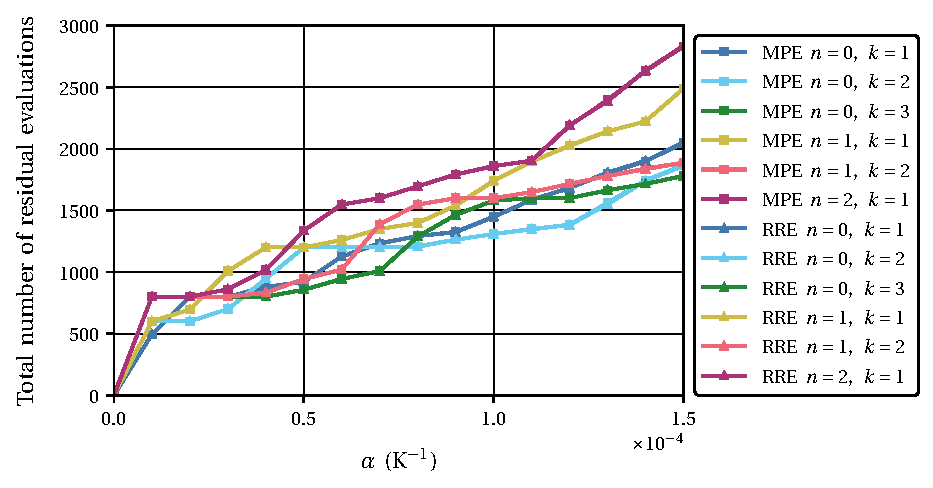
\includegraphics[width=0.9\textwidth]{thick_cylinder_extrap_pol_n_iter_coupl_strength_quad4fbar_pred}
  \caption{Total number of residual evaluations as a function of the thermal expansion coefficient for the polynomial vector extrapolation methods in cycling mode, MPE and RRE, restriced to at most five evaluations of the residual function per nonlinear iteration in the solution of the quasi-static expansion of a thermoelastic thick-walled cylinder with \(\alpha_T=\SIrange{0}{1.5e-4}{\kelvin^{-1}}\) and \(\dot u_0 =\SI{0.5}{\milli\meter\second^{-1}}\).}
\label{fig:thick_cylinder_extrap_pol_n_iter_coupl_strength_quad4fbar_pred}
\end{figure}

\FloatBarrier

\subsubsection{Comparison of the best methods in each class}

In this section, the best performing methods from each of the classes considered are compared with each other.
The implicit methods selected are the Aitken relaxation, Broyden's method with Type I update, a Broyden-like method with \(\beta=-1\) and \(s=2\), the Newton-GMRES method with \(\eta=\num{e-3}\) and the MPE in cycling mode with \((n,k)=(1,3)\).

Figure~\ref{fig:thick_cylinder_comparison_best_cpu_time_n_iter_coupl_strength_quad4fbar_pred} shows the total CPU time in seconds and the total number of residual evaluations as a function of the thermal expansion coefficient for the  best performing implicit methods in each class considered.
The best performing methods are Broyden's method and the Broyden-like method with \(\beta=-1\), followed by the Aitken relaxation, the MPE in cycling mode and the Newton-GMRES method.
As the thermal coefficient, and thus the strength of the coupling, increases, all the methods display a loss in efficiency.
Table~\ref{tab:res_cpu_nr_func_best} surmizes all the results previously discussed regarding the computational time taken by each of the solvers.

Figure~\ref{fig:thick_cylinder_comparison_best_time_profile_mesh_size_quad4fbar_pred} depicts the total CPU time in seconds, and time profile, as a function of the mesh size.
For all solvers and mesh sizes, the evaluation of the solvers is the operation that takes up the most computational time.
The computation of the residual function considered implies the solution of both the mechanical and thermal problem, with the mechanical solver taking longer than the thermal solver.
This can be explained in part because it has double the number of degrees of freedom.
Also the operations concerning the constitutive behavior of the material are performed in the mechanical solver for the implementation developed in this work.
The time spent on operations concerning solely the coupling solver, contribute a small weigth to the total time for all mesh sizes and solvers.
This happens despite the coupling between the mechanical and thermal problem being volumetric, leading to all the degrees of freedom in one of the solvers, in this case, in the thermal solver, to have to be considered by the coupling procedure.
This is in contrast to surface coupling, such as the one found fluid-structure interaction, where only the degrees of freedom at the contact surface need to be considered.

\begin{figure}[hbtp]
  \centering
  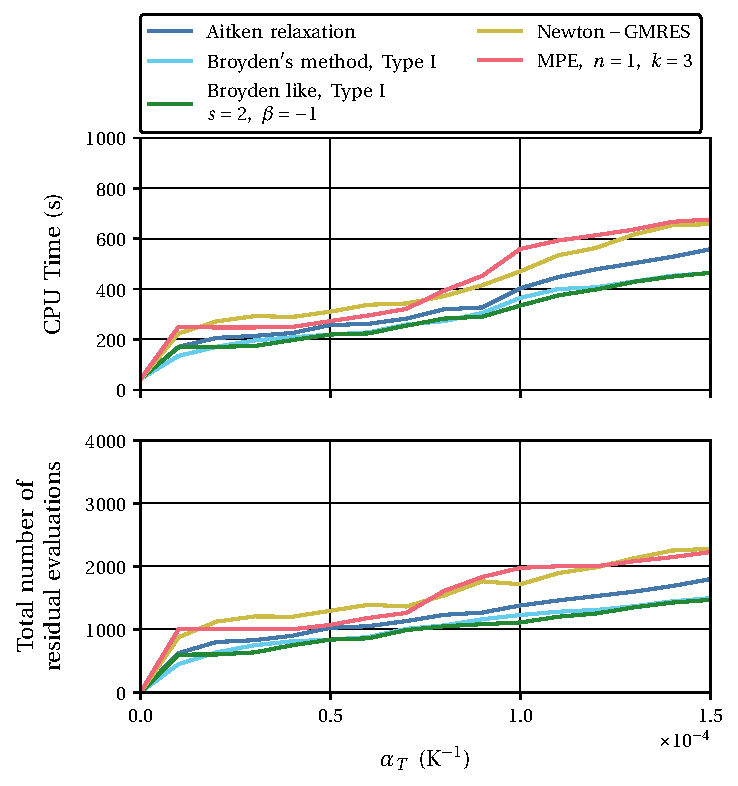
\includegraphics[width=.85\textwidth]{thick_cylinder_comparison_best_cpu_time_n_iter_coupl_strength_quad4fbar_pred}
  \caption{Total CPU time in seconds and total number of residual evaluations as a function of the thermal expansion coefficient for the  best performing implicit methods in each class considered in the solution of the quasi-static expansion of a thermoelastic thick-walled cylinder with \(\alpha_T=\SIrange{0}{1.5e-4}{\kelvin^{-1}}\) and \(\dot u_0 =\SI{0.5}{\milli\meter\second^{-1}}\).}
\label{fig:thick_cylinder_comparison_best_cpu_time_n_iter_coupl_strength_quad4fbar_pred}
\end{figure}

\begin{table}[hbtp]
  \centering
  \caption{Total CPU time in seconds and total number of residual evaluations as a function of the thermal expansion coefficient for the  best performing implicit methods in each class considered in the solution of the quasi-static expansion of a thermoelastic thick-walled cylinder with \(\alpha_T=\SIlist{5e-5; 10e-5; 15e-5}{\kelvin^{-1}}\), and \(\dot u_0 =\SI{0.5}{\milli\meter\second^{-1}}\).}
  \label{tab:res_cpu_nr_func_best}
  % \setlength{\tabcolsep}{3pt}
  \begin{tabular}
  {l
  S[round-mode=places, round-precision=2, table-format = 1.2e1]
  S[round-mode=places, round-precision=2, table-format = 1.2e1]
  S[round-mode=places, round-precision=2, table-format = 1.2e1]
  S[round-mode=places, round-precision=0, exponent-mode=fixed, fixed-exponent=0, table-number-alignment = center, table-format = 4.0]
  S[round-mode=places, round-precision=0, exponent-mode=fixed, fixed-exponent=0, table-number-alignment = center, table-format = 4.0]
  S[round-mode=places, round-precision=0, exponent-mode=fixed, fixed-exponent=0, table-number-alignment = center, table-format = 4.0] }
  \vphantom{\Big \vert}&  \multicolumn{3}{c}{CPU Time (\si{\second})} & \multicolumn{3}{c}{Nr Residual Evaluations} \\
  \cmidrule(lr){2-4}\cmidrule(lr){5-7}
  \vphantom{\Big \vert}\makecell[c]{$\alpha_T$\\ (\SI[exponent-mode=input]{1e-5}{\kelvin^{-1}})} & {5} & {10} & {15} & {5} & {10} & {15}\\
  \hline\hline
  \vphantom{\Big \vert}  AITK  & 2.57200e2 & 4.03400e2 & 5.58200e2 & 1.02500e+03 & 1.37800e+03 & 1.79600e+03\\
  \vphantom{\Big \vert}  BRDI  & \cellcolor{gray}2.19600e+02 & 3.64900e+02 & \cellcolor{gray}4.64000e+02 & \cellcolor{gray}8.36000e+02 & 1.22600e+03 & 1.49400e+03\\
  \vphantom{\Big \vert}  BRDI2  & \cellcolor{gray}2.19700e+02 & \cellcolor{gray}3.34600e+02 & 4.64500e+02 & \cellcolor{gray}8.36000e+02 & \cellcolor{gray}1.10800e+03 & \cellcolor{gray}1.46600e+03\\
  \vphantom{\Big \vert}  NEWT  & 3.10500e+02 & 4.70500e+02 & 6.57600e+02 & 1.29400e+03 & 1.71400e+03 & 2.27700e+03\\
  \vphantom{\Big \vert}  MPE  & 2.73100e+02 & 5.59100e+02 & 6.76100e+02 & 1.07000e+03 & 1.97500e+03 & 2.22500e+03\\


  \hline\hline
  \end{tabular}
\end{table}

\begin{figure}[hbtp]
  \centering
  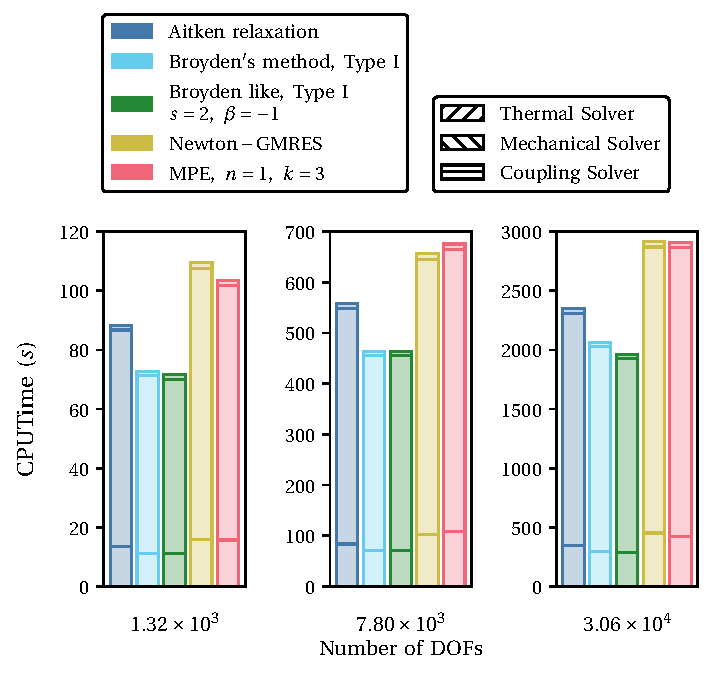
\includegraphics[width=.85\textwidth]{thick_cylinder_comparison_best_time_profile_mesh_size_quad4fbar_pred}
  \caption{Total CPU time in seconds, and time profile, as a function of the mesh size for the  best performing implicit methods in each class considered in the solution of the quasi-static expansion of a thermoelastic thick-walled cylinder with \(\alpha_T=\SI{1.5e-4}{\kelvin^{-1}}\) and \(\dot u_0 =\SI{0.5}{\milli\meter\second^{-1}}\).}
\label{fig:thick_cylinder_comparison_best_time_profile_mesh_size_quad4fbar_pred}
\end{figure}

\FloatBarrier

\subsubsection{Effect of predictiors}

Figure~\ref{fig:thick_cylinder_comparison_best_pred_total_iters_coupl_strength_quad4fbar_pred.pdf} presents the effect of employing a linear or quadratic predictor on the number of residual evalutions needed to fully solve the thermomechanical problem under analysis as a function of the thermal expansion coefficient.
All methods improve with the use of the polynomial predictors with the best effects being achieved using the quadratic predictor.
The decrease in the number of residual evaluations is around 30\% to 40\%.


\begin{figure}[hbtp]
  \centering
  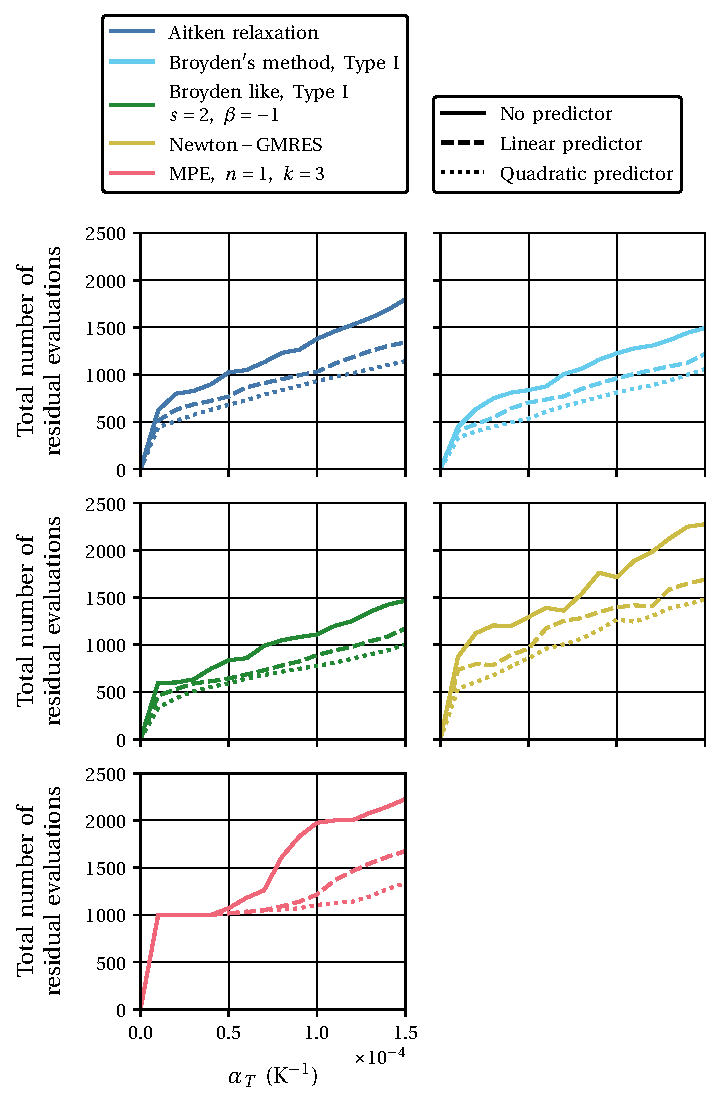
\includegraphics[width=.85\textwidth]{thick_cylinder_comparison_best_pred_total_iters_coupl_strength_quad4fbar_pred.pdf}
  \caption{Total number of iterations as a function of the thermal expansion coefficient for the  best performing implicit methods in each class considered using a linear, a quadratic and no predictor in the solution of the necking of a circular bar with \(\alpha_T=\SIrange{0}{1.5e-4}{\kelvin^{-1}}\) and \(\dot u_0 =\SI{0.5}{\milli\meter\second^{-1}}\).}
\label{fig:thick_cylinder_comparison_best_pred_total_iters_coupl_strength_quad4fbar_pred.pdf}
\end{figure}

\FloatBarrier

\pagebreak

\section{Necking of a circular bar}
\label{sec:mech-driv-probl}

The second validation example consists of the thermally triggered necking of a circular bar, as originally reported in \cite{simo_associative_1992} and replicated in \cite{danowski_computational_2014}.
The problem consists of a cylindrical bar of radius $r=\SI{6.413}{\milli\meter}$ and length $h=\SI{53.334}{\milli\meter}$ subject to a prescribed axial displacement $\bar{u}_{y}=\SI{8}{\milli\meter}$ at both ends during $t=\SI{8}{\second}$.
The supports at the tips allow transverse contraction of the specimen.
The bar is initially at the ambient temperature $T_{0}=T_{\infty}=\SI{293}{\kelvin}$ and is subject to heat transfer by convection at all boundaries, with a heat transfer coefficient $h_{c} = \SI{17.5e-3}{\newton\per\milli\meter\per\second\per\kelvin}$.
The material is modelled with the constitutive model by \cite{simo_associative_1992} and the material properties are given in Table~\ref{tab:matpropsnecking}.
%
\begin{table}
  \centering
  \caption{Material properties, and initial and boundary conditions for the problem concerning the quasi-static finite strain thermo-elastic expansion of an infinitely long thick-walled cylinder.}
\label{tab:matpropsnecking}
  \begin{tabular}{lccS[exponent-mode=engineering]}
  \multicolumn{3}{l}{Material Properties} & {\vphantom{\Big |}Effective value}\\
  \hline\hline
  \vphantom{\Big |}Density & \(\rho\) & (\si{\newton\second^2\milli\meter^{-4}}) & 7.8e-9\\
  \vphantom{\Big |}Bulk modulus & \(\kappa\) & (\si{\newton\milli\meter^{-2}}) & 164206\\
  \vphantom{\Big |}Shear modulus & \(\mu\) & (\si{\newton\milli\meter^{-2}}) & 801938\\
  \vphantom{\Big |}Conductivity & \(k\) & (\si{\newton\second^{-1}\kelvin^{-1}}) & 45\\
  \vphantom{\Big |}Heat capacity & \(C_V\) & (\si{\milli\meter^2\second^{-2}\kelvin^{-1}}) & 460e6\\
  \vphantom{\Big |}Coefficient of thermal expansion & \(\alpha_T\) & (\si{\kelvin^{-1}}) & 10e-6\\
  \vphantom{\Big |}Dissipation factor & \(\chi\) & (-) & 900e-3\\
  \vphantom{\Big |}Initial yield stress at \(T_0\) & \(\sigma_{y,0}\) & (\si{\newton\milli\meter^{-2}}) & 450\\
  \vphantom{\Big |}Linear hardening coefficient at \(T_0\) & \(H\) & (\si{\newton\milli\meter^{-2}}) & 129.24\\
  \vphantom{\Big |}Saturation exponent & \(\delta\) & (-) & 16.93\\
  \vphantom{\Big |}Saturation yield stress at \(T_0\) & \(\sigma_{y,\infty}\) & (\si{\newton\milli\meter^{-2}}) & 715\\
  \vphantom{\Big |}Thermal softening parameter (\(\sigma_{y,0}\)) & \(\omega_0\) & (\si{\kelvin^{-1}}) & 2e-3\\
  \vphantom{\Big |}Thermal softening parameter (\(\sigma_{u,\infty}, H\)) & \(\omega_h\) & (\si{\kelvin^{-1}}) & 2e-3\\
  \hline
  \multicolumn{3}{l}{Boundary Conditions\vphantom{\Big |}} & \\\hline
  \vphantom{\Big |}Radius of the cylindrical bar & \(r\) & (\si{\milli\meter}) & 6.413\\
  \vphantom{\Big |}Length of the cylindrical bar & \(h\) & (\si{\milli\meter}) & 53.334\\
  \vphantom{\Big |}Maximum displacement at both ends & \(\bar u_y\) & (\si{\milli\meter}) & 8\\
  \vphantom{\Big |}Time to maximum displacement & \(t\) & (\si{\second}) & 8\\
  \vphantom{\Big |}Heat transfer coefficient & \(h_c\) & (\si{\newton\milli\meter^{-1}\kelvin^{-1}}) & 17.5e-3\\
  % \multicolumn{3}{l}{\vphantom{\Big |}All mechanical degrees of freedom fixed in the \(y\)- and \(z\)-directions.}\\
  \hline
  \multicolumn{3}{l}{Initial Conditions\vphantom{\Big |}} & \\\hline
  Intial temperature & \(T_0\) & (\si{\kelvin}) & {293}\\
  \hline
  \multicolumn{3}{l}{Reference value \vphantom{\Big |}} & \\\hline
  \vphantom{\Big |}Temperature at outer radius (\(r=r_0\)) & (\si{\kelvin}) & \\
  \hline\hline
  \end{tabular}
\end{table}

%
This classical benchmark in isothermal elastoplasticity renders a bifurcation problem where the necking phenomenon is typically triggered by a geometric imperfection.
In the thermomechanical version, the combination of plastic dissipation in the bulk and heat transfer at the boundaries produce a temperature field that becomes progressively more heterogeneous during the loading.
With growing elongation, the temperature rise in the centre of the bar will increase relative to the exterior boundary and automatically trigger the necking, even for a geometrically perfect setup.

The problem is analysed using two-dimensional axisymmetric, QUAD4 elements for both the mechanical and the thermal problem.
Figure~\ref{fig:necking} illustrates the problem setup, the finite element mesh employed in the 2D simulations and characteristic stages of deformation and temperature field during the prescribed elongation, evidencing the significant necking of the bar.
%
\begin{figure}[p]
  \centering
  \def\svgwidth{1.0\linewidth}
  \footnotesize
  \input{figures/necking2.pdf_tex}
  \caption{Description of the thermally triggered necking of a circular bar problem, characteristic deformation and temperature field stages during the loading and example axisymmetric finite element mesh. The results represented have been obtained with QUAD4 elements, non-adiabatic boundary conditions, the inconsistent mechanical dissipation formulation and the Fourier law based on constant $k_{0}$.}
  \label{fig:necking}
\end{figure}
%
Only one-quarter of the specimen is simulated, resulting in a finite element mesh with 1326 nodes and 1250 elements.
Except where explicitly indicated, this is the mesh employed.
The load is applied in 80 equal time steps $\Delta t = \SI{0.1}{\second}$.
A quasi-static solution is computed for the mechanical problem using a backward Euler integration and the transient temperature field is integrated in time with the generalised-$\alpha$ method with $\rho_{\infty,T}=1.0$.

\subsection{Validation of the Numerical Results}

As validation for the results presented in the present work, the reaction force at the supports and the neck surface temperature at point A are compared to results found in the literature, see \ref{fig:necking}.
Different reference data is included in the analysis, in particular, the adiabatic and non-adiabatic results presented in the original work by \cite{simo_associative_1992} and the non-adiabatic results presented in \cite{danowski_computational_2014}.
It should be remarked that there are five fundamental differences between these two publications that lead to distinct results.
First, in \cite{simo_associative_1992}, the authors adopt a mechanical dissipation term that is thermodynamically inconsistent, based on the previously mentioned dissipation factor, $\chi$, whereas, in \cite{danowski_computational_2014}, the authors use the mechanical dissipation coming directly from the second law of thermodynamics.
Second, \cite{danowski_computational_2014} also uses a consistent structural heating term for the Gough-Joule effect, accounting for both elastic and plastic contributions.
In contrast, \cite{simo_associative_1992} considered the elastic contributions, exclusively.
For more information on the previous classification and mathematical formulas for the heating parcels, the reader is referred to \ref{cha:simo-miehes-thermo}.
The third difference is linked to the heat conduction law employed in each contribution.
Although the large deformation version of the Fourier law underlies both publications, \cite{simo_associative_1992} considered as a fixed material parameter the spatial thermal conductivity, $k$, and in \cite{danowski_computational_2014}, the material thermal conductivity, $k_{0}$, was instead interpreted as the fixed material parameter.
Without further mention, the latter is employed in the current work.
Fourth, \cite{simo_associative_1992} solved the coupled problem using an operator split scheme and \cite{danowski_computational_2014} pursued a monolithic solution.
Last, regarding  spatial discretisation, \cite{danowski_computational_2014} used HEXA8-FBAR elements and \cite{simo_associative_1992} employed mixed displacement-pressure QUAD8 elements.

To enable a fair comparison with the reference data, the numerical solution is calculated using both the adiabatic and non-adiabatic setups.
Furthermore, in the latter, the consistent and inconsistent interpretations are considered, including a calculation with fixed $k$.
The evolution of the reaction force and neck surface temperature as a function of the prescribed displacement are shown in \ref{fig:necking-results} for the 2D and 3D solutions, respectively.
\begin{figure}[!p]
  \centering
  % \includegraphics[width=1.0\linewidth]{./solution-techniques-thermomechanics/figures/necking/necking_results.pdf}
  \caption{Evolution of the reaction force at the tips of the bar and the neck surface temperature with the prescribed displacement using QUAD8 elements with reduced integration (QUAD8R) and HEXA8-FBAR elements.}
  \label{fig:necking-results}
\end{figure}
%
From a physical interpretation standpoint, the plot of reaction forces suggests that the simulation occurs almost entirely in the elastoplastic regime.
The necking process does not occur in the isothermal and adiabatic solutions, with the adiabatic solution predicting slightly smaller reactions due to the thermal softening effect.
Also, in this case, the temperature evolves uniformly in the bar and grows in a nearly linear fashion over time, as captured in the numerical solutions.
As previously postulated, the necking is automatically triggered in the non-adiabatic solutions, which produces a heavy reduction in the reaction force starting approximately at $\bar{u}_{y}=\SI{4}{\milli\meter}$, followed by a steep temperature rise due to the higher plastic dissipation.

Inspecting \ref{fig:necking-results} from a validation perspective, the numerical results show a good agreement with the literature.
The correlation between the non-adiabatic, inconsistent solution and fixed $k$ with the results from \cite{simo_associative_1992} is very satisfactory, both on the temperature and the reaction force side.
Curiously, while the reaction force seems almost insensitive to the element type employed, the neck temperature is better approximated with the QUAD8 solution, especially near the maximum displacement.
The slight difference observed between these cases can presumably be attributed to the distinct element technology and coupling solution strategy used to obtain the two curves.
Relative to the solutions based on the consistent mechanical heating, the numerical results show good agreement with the curves extracted from \cite{danowski_computational_2014} up to $\bar{u}_{y}=\SI{3}{\milli\meter}$, but features significant differences from there on, both in the mechanical and thermal responses.
The results are still consistent insofar as the numerical solution obtained in this solution predicts a smaller temperature increase but larger reaction forces, as the thermal softening is less pronounced.
Unfortunately, to the author's knowledge, there are no other bibliographical sources that consider the fully consistent thermomechanical version of the model to support any of the sides.
Nevertheless, as the accuracy relative to the results from \cite{simo_associative_1992} is already adequate, the possibly remaining issue resides at the constitutive model level and therefore does not compromise the coupling environment.
It should also be remarked that if the prescribed displacement is slightly larger, the weakly coupled partitioned solution diverges at some point.
This can be expected from the mathematical properties associated with this type of strategy, as discussed in this chapter.
In truth, numerical divergence can be observed to start near $\bar{u}_{y}=\SI{8}{\milli\meter}$ for the non-adiabatic, inconsistent solution, see \ref{fig:necking-results}.
In principle, it is possible to stabilise the solution by employing more advanced techniques, for instance, implicit coupling strategies with numerical acceleration.
Despite being paramount for a robust computer simulation tool, these topics are postponed to future developments.
Overall, the present results are a sound indication of the correct implementation of the coupling environment, in particular, the data exchange and solution orchestration.
\begin{figure}
% 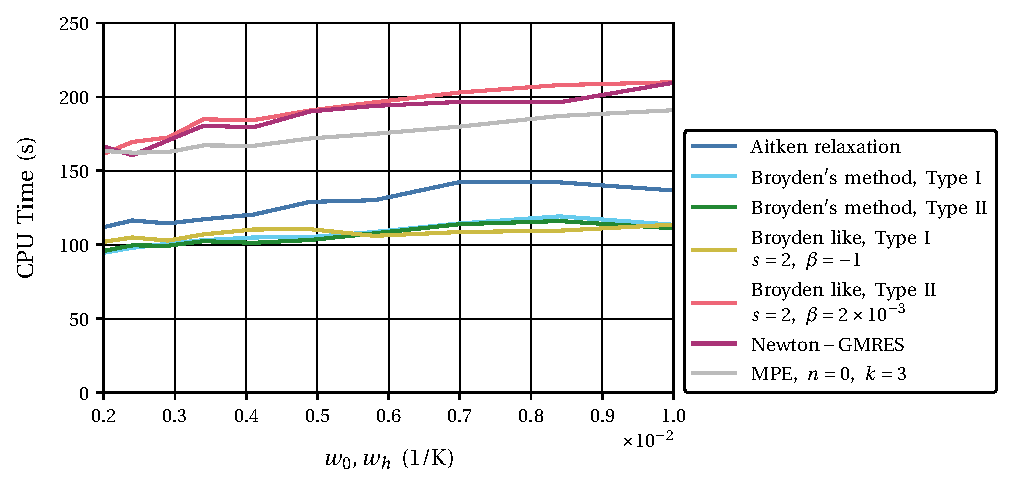
\includegraphics[width=.85\textwidth]{necking_comparison_methods_best_cpu_time_coupl_strength_quad4fbar_pred}
\end{figure}

\begin{figure}
% 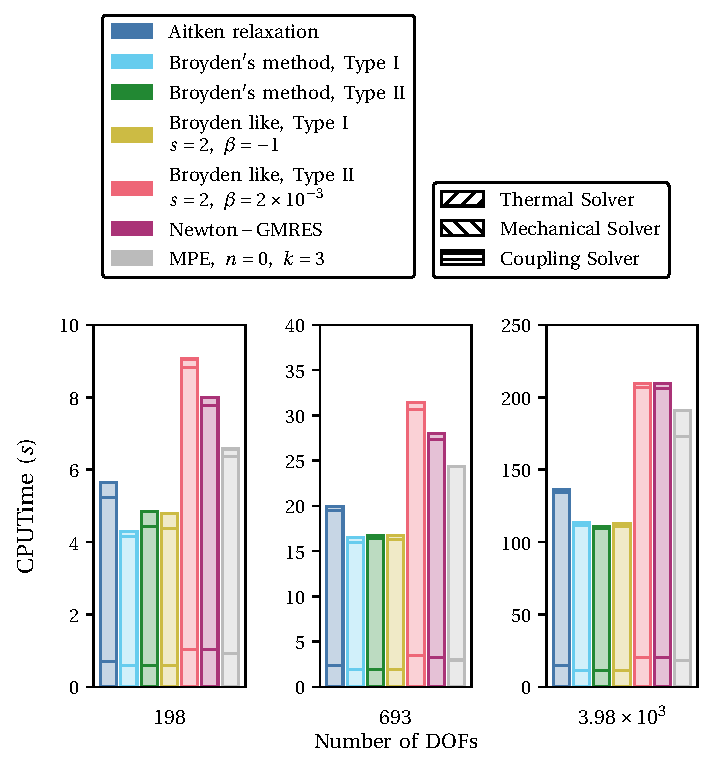
\includegraphics[width=.85\textwidth]{necking_comparison_methods_best_time_profile_mesh_size_quad4fbar_pred}
\end{figure}

\FloatBarrier

\subsection{Evaluation and comparison of implicit solution methods for the coupled problem}

The following contains the results concerning the evaluation and comparison of the implicit solution methods for coupled problems considered in this work.
The discussion starts with the methods that require only one evalution of the residual, implicitly requiring the solution of both the thermal and the mechanical problems by the corresponding solvers, per nonlinear iteration.
The Broyden-like family of methods fall into this category too but are considered by themselves and are presented next.
The Newton-Krylov methods are also analysed, followed by the vector extrapolation methods with cycling.
The discussion ends with the comparison bewteen the best methods in each class.

The analysis presented is based mainly on four pieces of information.
The first concerns how the residual evolves as a function of the nonlinear iterations.
The second is the number of function evaluations needed to solve the coupled problem to the desired accuracy at each time step.
The third is the total number of residual evaluations needed to solve the coupled problem to the desired accuracy as a function of the thermal softening parameters, \(w_0\) and \(w_h\), set to be equal.
The larger the softening parameters \(w_0\) and \(w_h\) the stronger the coupling between the thermal and mechanical fields, and the harder the problem is to solve.

The maximum displacement at both ends is restricted to \SI{5}{\milli\meter} applied in \SI{5}{\second} to prevent an excessive elongation of the elements in finite element simulation that often leads to simulation failure.
The thermal softening parameters \(w_0\) and \(w_h\) vary from \SIrange{2e-3}{1e-2}{\kelvin^{-1}}.
The larger the thermal softening parameters \(w_0\) and \(w_h\) the stronger the coupling.
This can be understood from Figure~\ref{fig:necking_single_iter_diff_w_0_n_iter_time_quad4fbar_pred}.
It shows the total number of residual evaluations, in this case corresponding also to the total number of nonlinear iterations, as a function of the thermal softening for the fixed-point method.
As \(w_0\) increases the displacement at which the coupling is the strongest moves to the left and the width of the corresponding peak gets larger, emplying a stronger coupling.

\begin{figure}[htbp]
  \centering
  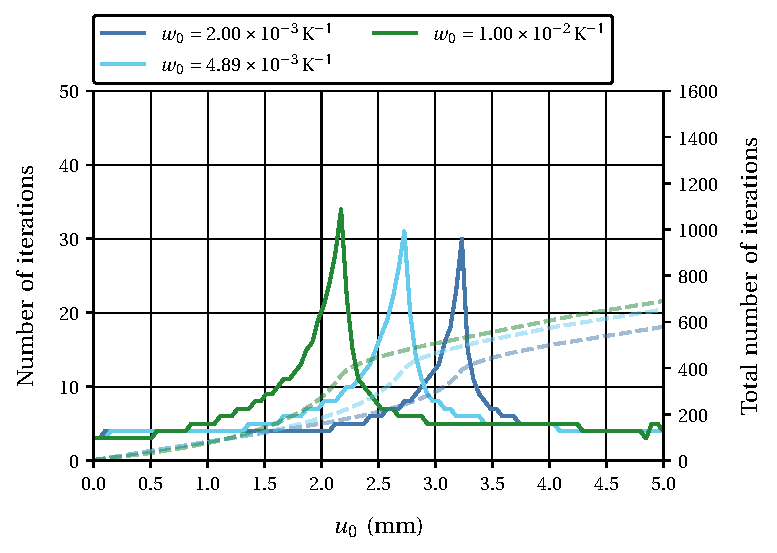
\includegraphics[width=.85\textwidth]{necking_single_iter_diff_w_0_n_iter_time_quad4fbar_pred}
  \caption{Total number of residual evaluations as a function of the thermal expansion coefficient for the fixed-point method in the solution of the necking of a circular bar with \(w_0=w_h=\SIlist{2e-3; 4.89e-3; 1e-2}{\kelvin^{-1}}\).}
\label{fig:necking_single_iter_diff_w_0_n_iter_time_quad4fbar_pred}
\end{figure}

\subsubsection{Methods with only one residual evaluation per iteration}

The methods with only one residual evaluation per nonlinear iteration considered are the fixed-point method (see Section~\ref{sec:fixed_point_approach}), the underrelaxation method (see Section~\ref{sec:underrelaxation}), the Aitken relaxation (see Section~\ref{sec:aitken_relaxation}) and Broyden's method, Type I and II (see Section~\ref{sec:multisecant}).
These are, a priori, the most parcimonious methods regarding residual evaluations, as only one is performed per nonlinear iteration.
The underrelaxation is performed with \(\omega = 0.5\), and the first relaxation coefficient for the Aitken relaxation is also set to 0.5.

Figure~\ref{fig:necking_single_iter_n_iter_time_quad4fbar_pred} presents the number of nonlinear iterations/residual evaluations needed to solve the coupled thermomechanical problem at each time step and the total (cumulative) number of iterations needed with \(w_0=w_h=\SI{1e-2}{\kelvin^{-1}}\).
It is clear from the number of nonlinear iterations needed to solve the problem at \(u_y\approx\SI{2.3}{\milli\meter}\), that the coupling is the strongest at this moment.
It corresponds to the moment where the necking of the bar begins.
There is a marked performance difference between the methods under analysis, with the Broyden methods taking a lot less iterations, 10, than either the Aitken relaxation, 18, or the fixed-point method, 34.
For all other moments, the performance of the implicit methods under analysis is very similar, except for the underrelaxation.
This is probably due to the poor choice of the relaxation coefficient.

\begin{figure}[htbp]
  \centering
  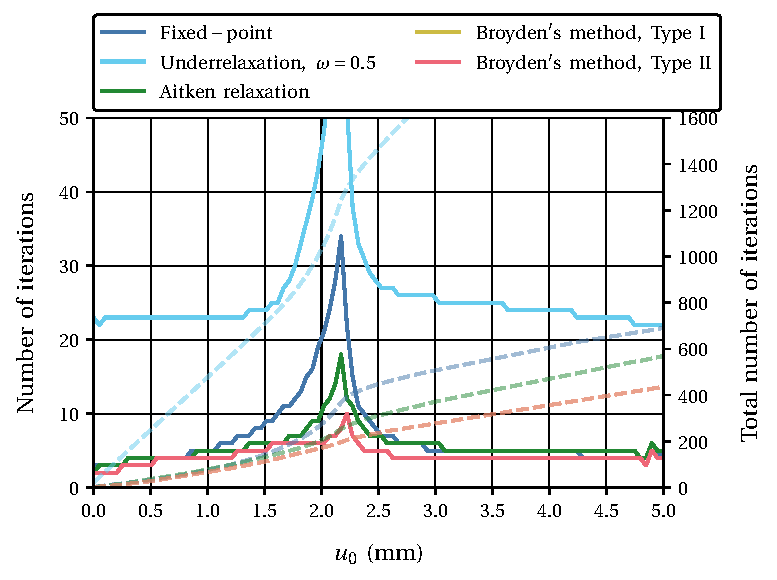
\includegraphics[width=.85\textwidth]{necking_single_iter_n_iter_time_quad4fbar_pred}
  \caption{Number of nonlinear iterations needed to solve the coupled problem at each time step and the total number of iterations needed to solve the coupled problem for the implicit methods that perform only one evaluation per nonlinear iteration in the solution of the necking of a circular bar with \(w_0=w_h=\SI{1e-2}{\kelvin^{-1}}\).}
\label{fig:necking_single_iter_n_iter_time_quad4fbar_pred}
\end{figure}

Figure~\ref{fig:necking_single_iter_n_iter_coupl_strength_quad4fbar_pred} presents the total number of residual evaluations, in this case corresponding also to the total number of nonlinear iterations, as a function of the thermal softening parameters, which control sthe strength of the coupling between the thermal and the mechanical fields, respectively.
The most efficient methods are the two Broyden methods, followed by the Aitken relaxation.
The difference bewteen the total number of iterations is around 100 for the three different methods.

\begin{figure}[htbp]
  \centering
  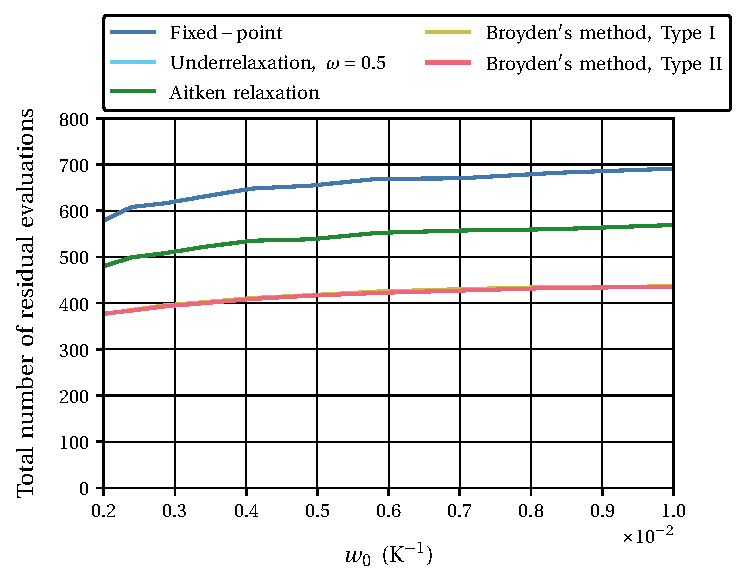
\includegraphics[width=.85\textwidth]{necking_single_iter_n_iter_coupl_strength_quad4fbar_pred}
  \caption{Total number of residual evaluations as a function of the thermal expansion coefficient for the implicit methods that perform only one evaluation per nonlinear iteration in the solution of the necking of a circular bar with \(w_0=w_h=\SIrange{2e-3}{1e-2}{\kelvin^{-1}}\).}
\label{fig:necking_single_iter_n_iter_coupl_strength_quad4fbar_pred}
\end{figure}

\FloatBarrier

\subsubsection{Broyden-like method}

The Broyden-like methods considered (see Section~\ref{sec:multisecant}) employ as group sizes \(s=1,\ 2,\ 3,\ 6\) with a maximum number of previous iterations available equal to 6.
The mixing parameters considered are \(\beta=-1,\ \num{2e-3},\ \num{2e-2}\).
All combinations are also considered with both Type I and Type II updating for the approximation to the Jacobian.

Figures~\ref{fig:necking_broyden_like_type_i_n_iter_time_quad4fbar_pred} and \ref{fig:necking_broyden_like_type_ii_n_iter_time_quad4fbar_pred} present the number of nonlinear iterations/number of function evaluations needed to solve the coupled problem at each time step and the total (cumulative) number of iterations needed in the solution of the necking of a circular bar with \(w_0=w_h=\SI{1e-2}{\kelvin^{-1}}\).
Regarding the methods using \(\beta=-1\), the difference bewteen Type I and II methods is not noticeable.
However, the different size groups lead to different behaviors.
For the displacement values where the coupling is the weakest, a larger group size leads to worse results.
On the other hand, the number of iterations where the coupling is the strongest are about the same for all group sizes.
For \(\beta=\num{2e-3}\) and \num{2e-2} the only group size that converges is \(s=6\).
For the other group sizes, the simulation breaks down approxitameltly after reaching \(u_y=\SI{2.3}{\milli\meter}\).
This happens because the mechanical solver fails with an exploding residual in its internal Newton-Raphson procedure.
It doesn't seem to be directly related to the coupling solver itself.

\begin{figure}[htbp]
  \centering
  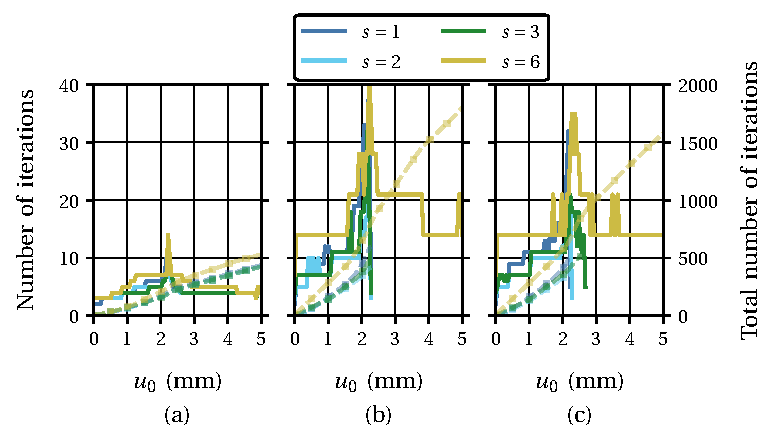
\includegraphics[width=.85\textwidth]{necking_broyden_like_type_i_n_iter_time_quad4fbar_pred}
  \caption{
Number of nonlinear iterations needed to solve the coupled problem at each time step and the total number of iterations needed to solve the coupled problem for Broyden-like methods with Type I update and group sizes \(s=1\), 2, 4 and 6: (a) \(\beta=-1\), (b) \(\beta=\num{2e-3}\), and (c) \(\beta=\num{2e-2}\) in the solution of the necking of a circular bar with \(w_0=w_h=\SI{1e-2}{\kelvin^{-1}}\).}
\label{fig:necking_broyden_like_type_i_n_iter_time_quad4fbar_pred}
\end{figure}

\begin{figure}[htbp]
  \centering
  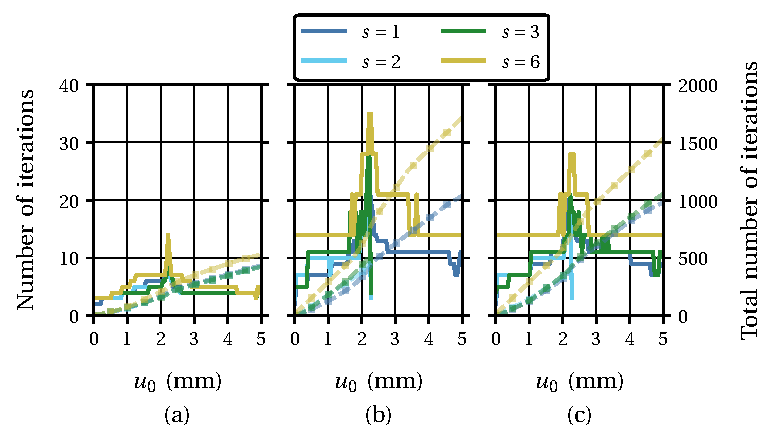
\includegraphics[width=.85\textwidth]{necking_broyden_like_type_ii_n_iter_time_quad4fbar_pred}
  \caption{Number of nonlinear iterations needed to solve the coupled problem at each time step and the total number of iterations needed to solve the coupled problem for Broyden-like methods with Type II update and group sizes \(s=1\), 2, 4 and 6: (a) \(\beta=-1\), (b) \(\beta=\num{2e-3}\), and (c) \(\beta=\num{2e-2}\) in the solution of the necking of a circular bar with \(w_0=w_h=\SI{1e-2}{\kelvin^{-1}}\).}
\label{fig:necking_broyden_like_type_ii_n_iter_time_quad4fbar_pred}
\end{figure}

Figures~\ref{fig:necking_broyden_like_type_i_n_iter_coupl_strength_quad4fbar_pred} presents the total number of residual evaluations as a function of the thermal softening parameter, respectively, for the Broyden-like methods with Type I update considered.
The same results are presented in Figures~\ref{fig:necking_broyden_like_type_ii_n_iter_coupl_strength_quad4fbar_pred} for the Broyden-like methods with Type II update.
For \(\beta=-1\), the best results are obtained for \(s=\SIlist{1; 2; 3}{}\).
However, for \(s=3\) convergence is not always achieved.
For \(\beta=\num{2e-3}\) and \num{2e-3} the best results seem to be obtained for \(s=2\) when the methods do converge.
However, this is a rare occurence.

\begin{figure}[htbp]
  \centering
  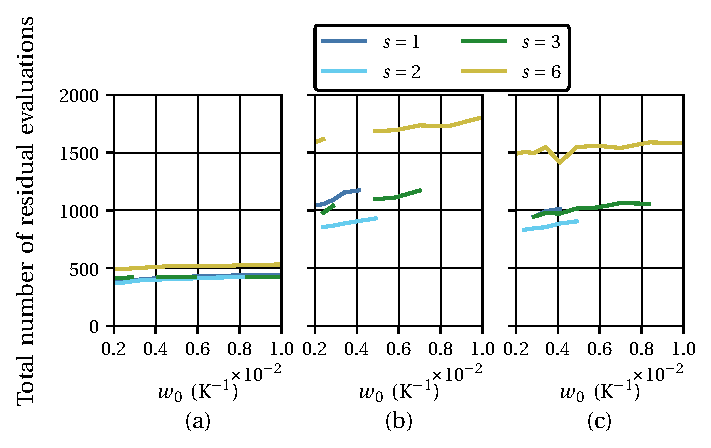
\includegraphics[width=.85\textwidth]{necking_broyden_like_type_i_n_iter_coupl_strength_quad4fbar_pred}
  \caption{Total number of residual evaluations as a function of the thermal expansion coefficient for the implicit methods for Broyden-like methods with Type I update and group sizes \(s=1\), 2, 4 and 6: (a) \(\beta=-1\), (b) \(\beta=\num{2e-3}\), and (c) \(\beta=\num{2e-2}\) in the solution of the necking of a circular bar with \(w_0=w_h=\SIrange{2e-3}{1e-2}{\kelvin^{-1}}\).}
\label{fig:necking_broyden_like_type_i_n_iter_coupl_strength_quad4fbar_pred}
\end{figure}

\begin{figure}[htbp]
  \centering
  \includegraphics[width=.85\textwidth]{necking_broyden_like_type_ii_n_iter_coupl_strength_quad4fbar_pred}
  \caption{Total number of residual evaluations as a function of the thermal expansion coefficient for Broyden-like methods with Type II update and group sizes \(s=1\), 2, 4 and 6: (a) \(\beta=-1\), (b) \(\beta=\num{2e-3}\), and (c) \(\beta=\num{2e-2}\) in the solution of the necking of a circular bar with \(w_0=w_h=\SIrange{2e-3}{1e-2}{\kelvin^{-1}}\).}
\label{fig:necking_broyden_like_type_ii_n_iter_coupl_strength_quad4fbar_pred}
\end{figure}

\FloatBarrier

\subsubsection{Newton-GMRES method}

The Newton-Krylov method examined here uses as the Krylov subspace solver the GMRES method (see Section~\ref{sec:newton_krylov}).
Different forcing terms are employed.
The values considered are \(\eta=\num[print-unity-mantissa=false]{e-1}\), \num[print-unity-mantissa=false]{e-3} and \num[print-unity-mantissa=false]{e-5}.
The Eisenstat-Walker scheme for the adpative choice of the forcing term is also utilized.

Figure~\ref{fig:necking_newton_krylov_n_iter_time_quad4fbar_pred} presents the number of nonlinear iterations needed to solve the coupled problem at each time step and the total (cumulative) number of iterations needed.
For the Newton-GMRES methods considered the moment where the coupling is the strongest is not as a clear as for the methods considered until now.
However, the number of iterations needed to solve the thermomechanical problem at each timestep is the largest for \(u_y = \SI{2.3}{\milli\meter}\).
Also, contrary, to the other methods, where the coupling is the weakest there is still some difference between the methods considered.
In general, higher forcing terms lead to less iterations.
Keep in mind, however, that less iteration doesn't necesseraly correspond to fewer residual evaluations.

\begin{figure}
  \centering
  \includegraphics[width=.85\textwidth]{necking_newton_krylov_n_iter_time_quad4fbar_pred}
  \caption{Number of nonlinear iterations needed to solve the coupled problem at each time step and the total number of iterations needed to solve the coupled problem for the Newton-GMRES method with a constant forcing term (\(\eta=\num{1e-5},\ \num{1e-3},\ \num{1e-1}\)) and the Eisenstat-Walker scheme in the solution of the necking of a circular bar with \(w_0=w_h=\SI{1e-2}{\kelvin^{-1}}\).}
\label{fig:necking_newton_krylov_n_iter_time_quad4fbar_pred}
\end{figure}

Figure~\ref{fig:necking_newton_krylov_n_iter_coupl_strength_quad4fbar_pred} present the total number of residual evaluations as a function of the thermal softening parameters \(w_0\) and \(w_h\).
The best performing method is the one employng a constant forcing term equal to \num{1e-3}.
The other constant forcing terms and the Eisenstat-Walker method display a similar efficiency.
The methods using a constant forcing also fail to converge for \(w_0=w_h=\SI{2e-3}{\kelvin^{-1}}\).

\begin{figure}
  \centering
  \includegraphics[width=.85\textwidth]{necking_newton_krylov_n_iter_coupl_strength_quad4fbar_pred}
  \caption{Total number of residual evaluations as a function of the thermal expansion coefficient for the Newton-GMRES method with a constant forcing term (\(\eta=\num{1e-5},\ \num{1e-3},\ \num{1e-1}\)) and the Eisenstat-Walker scheme in the solution of the necking of a circular bar with \(w_0=w_h=\SIrange{2e-3}{1e-2}{\kelvin^{-1}}\).}
\label{fig:necking_newton_krylov_n_iter_coupl_strength_quad4fbar_pred}
\end{figure}

\FloatBarrier

\subsubsection{Polynomial vector extrapolation in cycling mode}

The polynomial vector extrapolation methods in cycling mode considered are the MPE and RRE, restriced to at most five evaluations of the residual function per nonlinear iteration.
Thus, the combinations analyzed are characterized by the ordered pairs \((n,k)=(1,1)\), \((1,2)\), \((1,3)\), \((2,1)\), \((2,2)\) and \((3,1)\).

Figure~\ref{fig:necking_extrap_pol_n_iter_time_quad4fbar_pred} presents the number of residual evaluations needed to solve the coupled problem at each time step and the total (cumulative) number of iterations needed with \(w_0=w_h=\SI{1e-2}{\kelvin^{-1}}\).
There is no clear difference bewtween the MPE and the RRE.
The moment of strongest coupling is clearly visible for the methods using few residual evaluations per nonlinear iteration, such as \((n,k)=(1,1)\).
For \((n,,k)=(1,3)\), this is much less noticeable.
Regarding the moments, where the coupling is weaker, the difference bewteen the methods is less marked.

\begin{figure}[htbp]
  \centering
  \includegraphics[width=0.9\textwidth]{necking_extrap_pol_n_iter_time_quad4fbar_pred}
  \caption{Number of nonlinear iterations needed to solve the coupled problem at each time step and the total number of iterations needed to solve the coupled problem for the polynomial vector extrapolation methods in cycling mode, MPE and RRE, restriced to at most five evaluations of the residual function per nonlinear iteration in the solution of the necking of a circular bar with \(w_0=w_h=\SI{1e-2}{\kelvin^{-1}}\).}
\label{fig:necking_extrap_pol_n_iter_time_quad4fbar_pred}
\end{figure}

Figures~\ref{fig:necking_extrap_pol_n_iter_coupl_strength_quad4fbar_pred} present the total number of residual evaluations as a function of the thermal expansion coefficient.
The method which performs the best uses \((n,k)=(1,3)\).
The second and third best methods are also the ones using five residual evaluations per nonlinear iteration, \((n,k)=(2,2)\) and \((n,k)=(3,1)\).

\begin{figure}[htbp]
  \centering
  \includegraphics[width=0.9\textwidth]{necking_extrap_pol_n_iter_coupl_strength_quad4fbar_pred}
  \caption{Total number of residual evaluations as a function of the thermal expansion coefficient for the polynomial vector extrapolation methods in cycling mode, MPE and RRE, restriced to at most five evaluations of the residual function per nonlinear iteration in the solution of the necking of a circular bar with \(w_0=w_h=\SIrange{2e-3}{1e-2}{\kelvin^{-1}}\).}
\label{fig:necking_extrap_pol_n_iter_coupl_strength_quad4fbar_pred}
\end{figure}

\FloatBarrier

\subsubsection{Comparison of the best methods in each class}

In this section the best performing methods from each of the classes considered are compared with each other.
The implicit methods selected are Aitken relaxation, Broyden's method with Type I update, a Broyden-like method with \(\beta=-1\) and \(s=2\), the Newton-GMRES method with \(\eta=\num{e-3}\) and the MPE in cycling mode with \((n,k)=(1,3)\).

Figure~\ref{fig:necking_comparison_best_cpu_time_n_iter_coupl_strength_quad4fbar_pred} shows the total CPU time in seconds and the total number of residual evaluations as a function of the thermal softening parameters for the  best performing implicit methods in each class considered.
The best performing methods are Broyden's method and the Broyden-like method, whose performance is very similar.
Their are followed by the Aitken relaxation and the MPE in cycling mode, also displaying a comparable efficiency to each other.
The Newton-GMRES method is the worse performing method considered.
As the thermal softening parameters, and thus the strength of the coupling, increases, all the methods display approximately a similiar loss in efficiency.
Table~\ref{tab:necking_res_cpu_nr_func_best} surmizes all the results previously discussed regarding the computational time taken by each of the solvers.

\begin{figure}[hbtp]
  \includegraphics[width=.85\textwidth]{necking_comparison_best_cpu_time_n_iter_coupl_strength_quad4fbar_pred}
  \caption{Total CPU time in seconds an total number of residual evaluations as a function of the thermal softening parameters \(w_0=w_h\) for the  best performing implicit methods in each class considered in the solution of the necking of a circular bar with \(w_0=w_h=\SIrange{2e-3}{1e-2}{\kelvin^{-1}}\).}
\label{fig:necking_comparison_best_cpu_time_n_iter_coupl_strength_quad4fbar_pred}
\end{figure}

\begin{table}[hbtp]
  \centering
  \caption{Total CPU time in seconds and total number of residual evaluations as a function of the thermal softening parameters \(w_0=w_h\) for the  best performing implicit methods in each class considered in the solution of the necking of a circular bar with \(w_0=w_h=\SIlist{2e-3; 4.89e-3; 1e-2}{\kelvin^{-1}}\).}
  \label{tab:necking_res_cpu_nr_func_best}
  % \setlength{\tabcolsep}{3pt}
  \begin{tabular}
  {l
  S[round-mode=places, round-precision=2, table-format = 1.2e1]
  S[round-mode=places, round-precision=2, table-format = 1.2e1]
  S[round-mode=places, round-precision=2, table-format = 1.2e1]
  S[round-mode=places, round-precision=0, exponent-mode=fixed, fixed-exponent=0, table-number-alignment = center, table-format = 4.0]
  S[round-mode=places, round-precision=0, exponent-mode=fixed, fixed-exponent=0, table-number-alignment = center, table-format = 4.0]
  S[round-mode=places, round-precision=0, exponent-mode=fixed, fixed-exponent=0, table-number-alignment = center, table-format = 4.0] }
  \vphantom{\Big \vert}&  \multicolumn{3}{c}{CPU Time (\si{\second})} & \multicolumn{3}{c}{Nr Residual Evaluations} \\
  \cmidrule(lr){2-4}\cmidrule(lr){5-7}
  \vphantom{\Big \vert}\makecell[c]{$w_0$\\ (\SI[exponent-mode=input]{1e-3}{\kelvin^{-1}})} & {2} & {4.89} & {10} & {2} & {4.89} & {10}\\
  \hline\hline
  \vphantom{\Big \vert} AITK  & 1.51000e+02 & 1.73300e+02 & 1.92100e+02 & 4.80000e+02 & 5.38000e+02 & 5.69000e+02\\
  \vphantom{\Big \vert} BRDI  & 1.20100e+02 & 1.40700e+02 & 1.54900e+02 & 3.76000e+02 & 4.17000e+02 & 4.36000e+02\\
  \vphantom{\Big \vert} BRDI2  & \cellcolor{gray}1.17700e+02 & \cellcolor{gray}1.37100e+02 & \cellcolor{gray}1.48200e+02 & \cellcolor{gray}3.68000e+02 & \cellcolor{gray}4.07000e+02 & \cellcolor{gray}4.24000e+02\\
  \vphantom{\Big \vert} NEWT  & NC & 2.15400e+02 & 2.38500e+02 & 4.36000e+02 & 7.81000e+02 & 8.33000e+02\\
  \vphantom{\Big \vert} MPE  & 1.64100e+02 & 1.81300e+02 & 1.94300e+02 & 5.35000e+02 & 5.55000e+02 & 5.80000e+02\\

  \hline\hline
  \end{tabular}
\end{table}

\subsubsection{Effect of predictiors}

Figure~\ref{fig:necking_comparison_best_pred_total_iters_coupl_strength_quad4fbar_pred} presents the effect of employing a linear or quadratic predictor on the number of residual evalutions needed to fully solve the thermomechanical problem under analysis as a function of the thermal expansion coefficient.
All methods improve with the use of the polynomial predictors with the best effects being achieved using the quadratic predictor.
The decrease in the number of residual evaluations is around 30\% to 40\% for all methods when using the quadratic predictor, except for the MPE.
The polynomial vector extrapolation method display a much smaller increase in efficiency from the polynomial predictors considered.
Finally, the use of predictors allows the Newton-GMRES method to converge for \(w_0=w_h=\SI{2e-3}{\kelvin^{-1}}\).

\begin{figure}[hbtp]
  \includegraphics[width=.85\textwidth]{necking_comparison_best_pred_total_iters_coupl_strength_quad4fbar_pred}
  \caption{Total number of iterations as a function of the thermal softening parameters \(w_0=w_h\) for the  best performing implicit methods in each class considered using a linear, a quadratic and no predictor in the solution of the necking of a circular bar with \(w_0=w_h=\SIrange{2e-3}{1e-2}{\kelvin^{-1}}\).}
\label{fig:necking_comparison_best_pred_total_iters_coupl_strength_quad4fbar_pred}
\end{figure}

\FloatBarrier

% \include{conclusions}
\appendix
% \include{annex}

\bibliography{Thermomechanics.bib}

\end{document}
